\chapter{Search for long-lived HNL in final states
with three leptons and displaced vertices} \label{Chapter6} 

\section{Change of scenario}

So far an explicit signal of new physics from either direct or indirect
searches at the LHC, or direct detection of DM is
missing. Furthermore, theory presents no clear direction on the new physics scale.
This forces a refining and widening of the experimental effort
investigating into BSM scenarios. We should explore various ranges of
interaction strengths and masses in addition with respect to
what is already probed by the current experimental
settings and analyses.

Among the plethora of possible new physics theories, quite eccentric
possibility could be the introduction of long-lived particles (LLPs)
decaying in the detector or long-lived detector-stable particles which decay outside the detector volume. 
These two require a change of scenario with respect to the usual
searches for new physics probed until some years ago and they do require the
inclusion of unconventional signature searches.\\
Long-lived particles could be foreseen by several models due to:
\begin{itemize}
\setlength\itemsep{-0.1em}
\item \emph{small coupling constants} -- \ie HNLs, RPV SUSY (R-parity violating
  SUSY scenario), etc;
\item \emph{very off-shell intermediate decay products} -- \ie split SUSY where
heavy intermediate squarks enhance
the gluino lifetime~\cite{ATLAS-CONF-2019-006,2020135114};
\item \emph{limited decay phase space} --- \ie
anomaly mediated SUSY breaking
model where the lightest neutralino
and chargino are nearly degenerate~\cite{Sirunyan:2019wau,Sirunyan:2019gut}.
\end{itemize}

CMS and ATLAS were 
initially designed to optimize object
identification for prompt particles, thus to integrate displaced
signatures into CMS framework we have to face quite a diverse number
of challenges:
\begin{itemize}
\setlength\itemsep{-0.1em}
\item \emph{triggers}: timing information at trigger level is not always
  available and the majority of current triggers uses primary vertex
  seeds to identify the matching tracks;
\item \emph{reconstruction}: we need the possibility to use algorithms which
  fit the eventual secondary vertices and integrate such informations in the
  reconstruction procedure;
\item \emph{background}: additional sources of background have to be
  considered such as noise from the detector itself (instrumental
  background), cosmic rays traveling through CMS's barrel, in-time
  and out-of-time pileup and long-lived SM hadrons which
  could mimic the interesting BSM particle.
\end{itemize}

\subsection{Displaced signature at CMS}
In Figure~\ref{fig:c6antonelli} several exemplary displaced
signatures are shown.\\
If the LLP decays into charged objects, we can have visible secondary vertices
made either of displaced leptons or of displaced jets; in case the LLP decays into two $\gamma$,
then we should rely on the possibility of the CMS
ECAL to measure $\gamma$ arrival times with enough precision to detect
signatures of delayed photons produced at displaced
vertices~\cite{Sirunyan:2019wau}.
There is also the chance of having the LLP that decays within the
volume of the silicon tracker producing events with an isolated track
which "disappears'' \ie it misses hits in the outermost layers of the
silicon tracker, it is associated with little energy deposited in the
calorimeters and it does not show hits in the muon detectors~\cite{Sirunyan_2020disapp}. 
\begin{figure}[h]
\centering
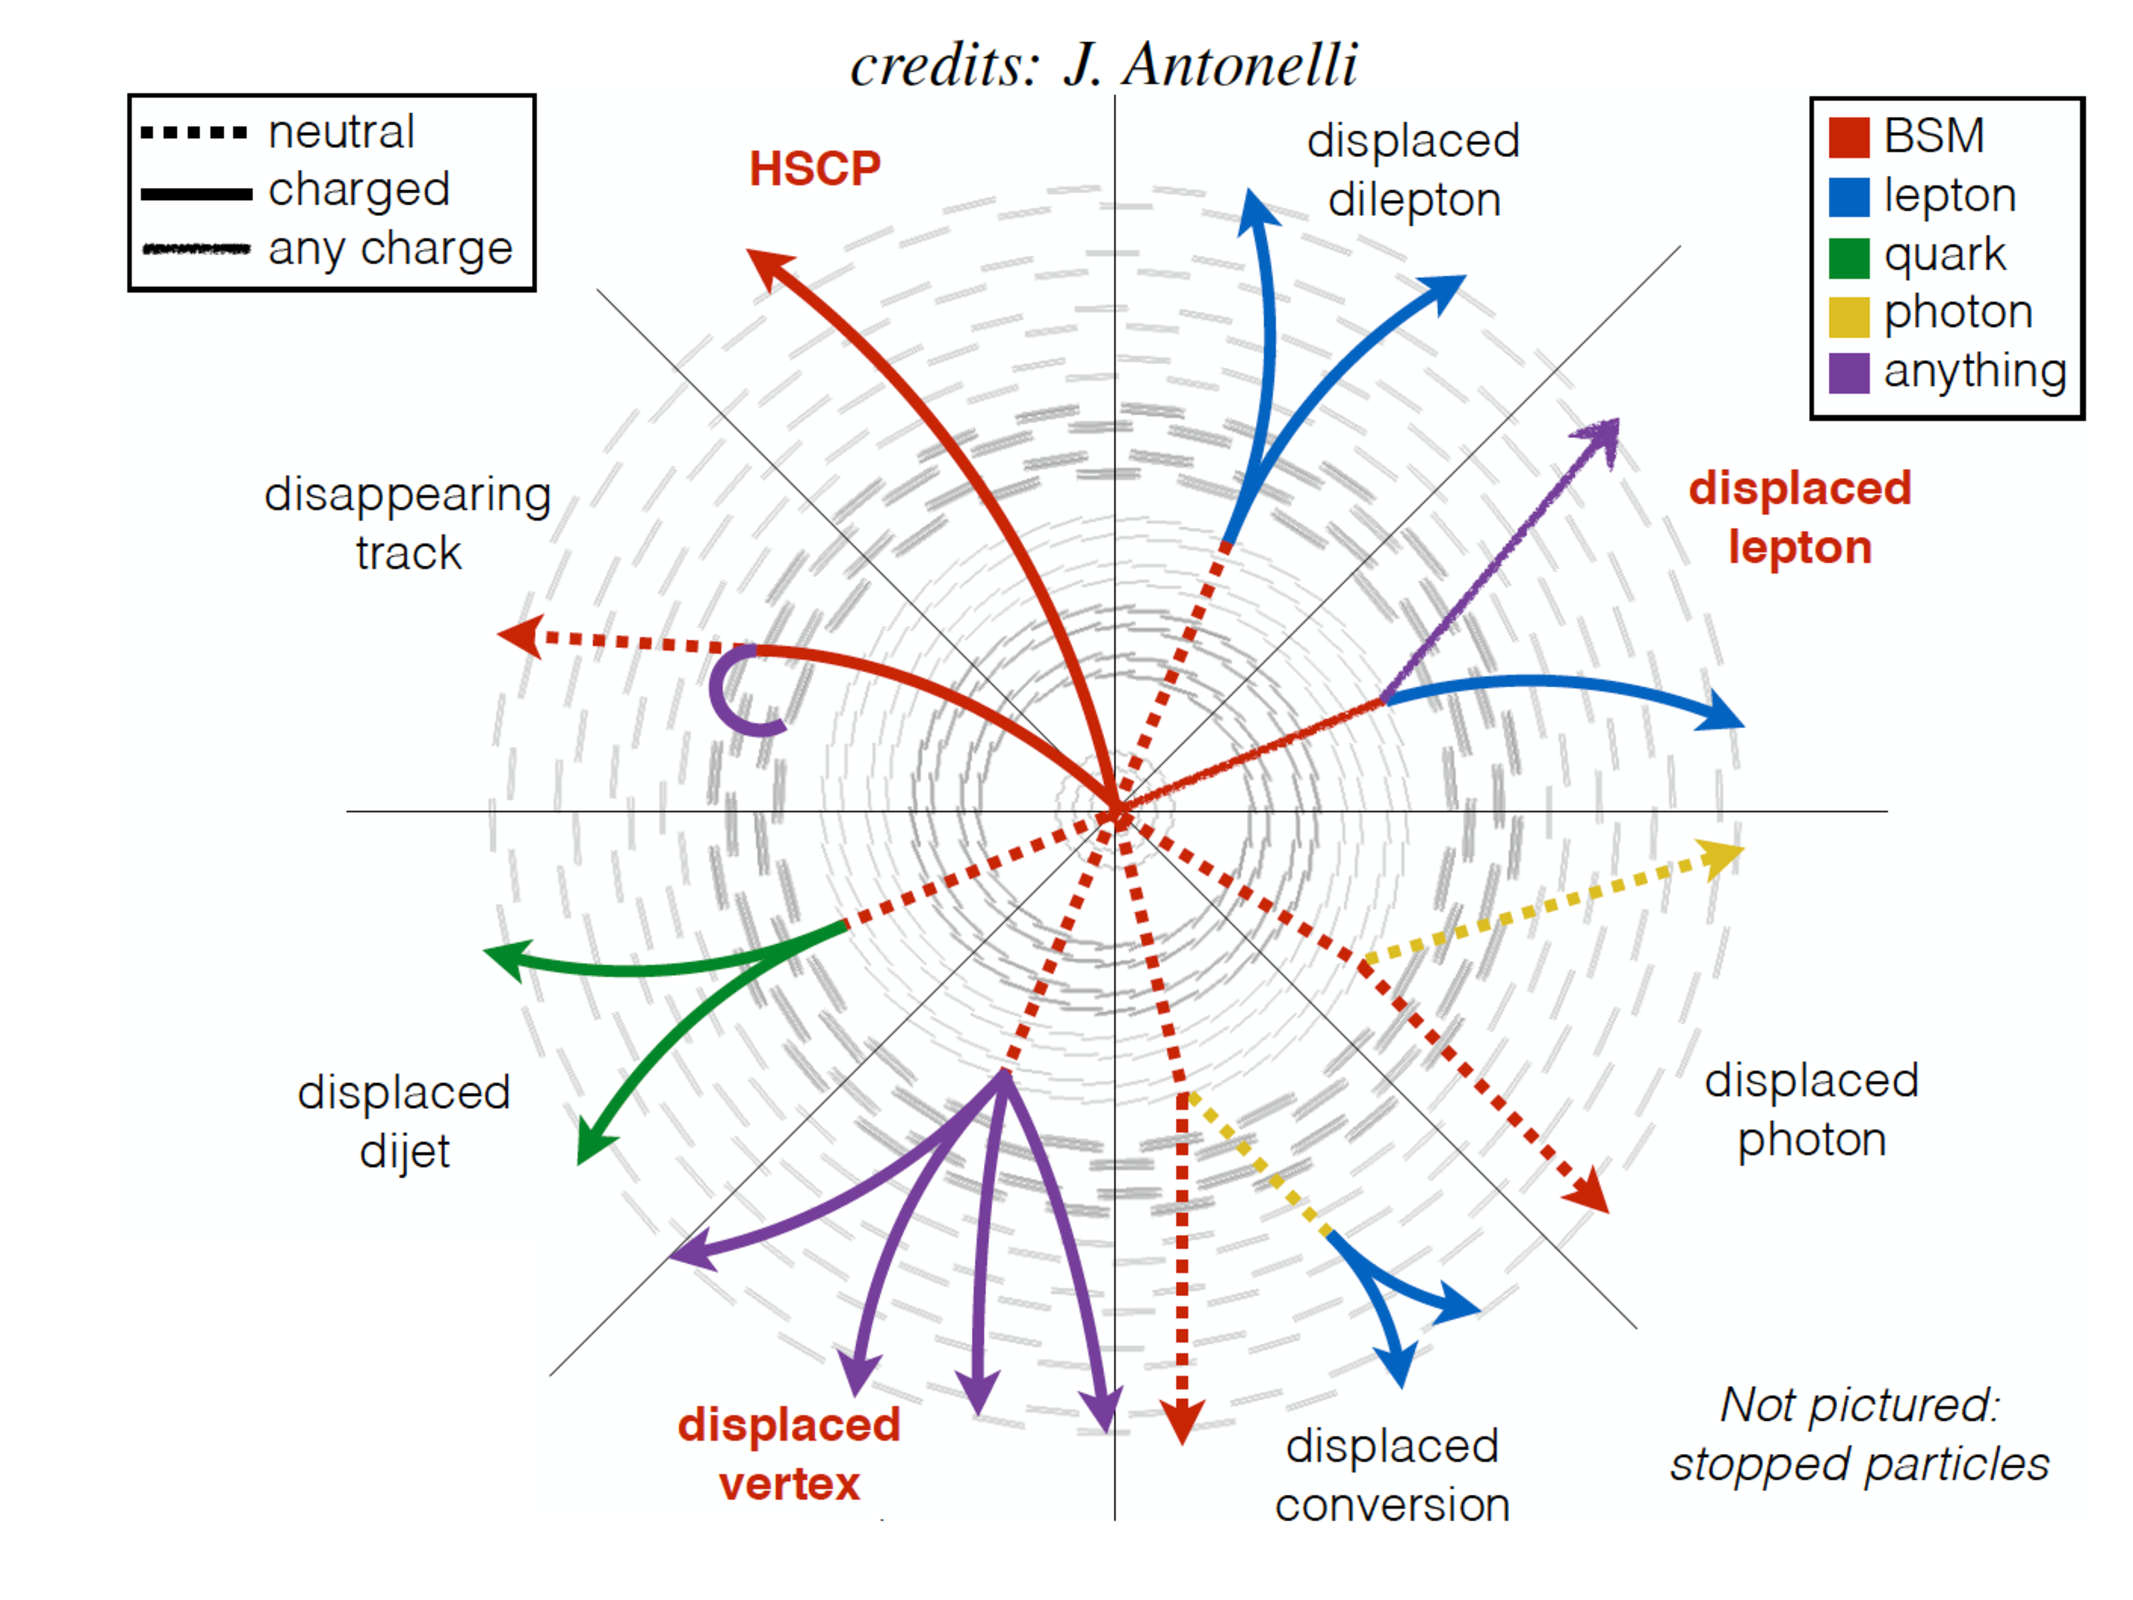
\includegraphics[clip,trim=0cm 0.cm 0.cm 1.6cm, width=0.85\textwidth]{Figures/c6/antonelli_skech.pdf}
\caption{Didactic sketch, by J. Antonelli, showing the numerous
  experimental signatures in the CMS tracker from various hypothetical particles proposed in long-lived models. }
\label{fig:c6antonelli}
\end{figure}

These are just few examples of the almost endless configurations which can
be studied including the \emph{long-lived} particle signatures in the
current particle physics searches. 

\subsubsection{HNL with long lifetime}
Along these lines, extending the HNL search described in
Chapter~\ref{Chapter5} including the long-lived HNL decays it feels like a logical
continuation. 

Recalling the considerations illustrated in Section~\ref{sec:promptll}, the lifetime of a HNL is strongly dependent on \mhnl and \mixpar,
and it increases rapidly at small masses and low values of the mixing
parameter (see Figure~\ref{fig:hnlLifetime}):
\(\tau_\hnl\propto\mathrm{\mhnl^{-5}|V_{\hnl\ell}|^{-2}}.\)
As a result, the kinematics and the acceptance of HNLs with masses
below about 20\GeV are significantly affected by their long lifetimes,
and must be accounted for in the signal simulation and in the results'
interpretation.
If $\hnl$ has a long lifetime, then a secondary vertex formed by the decay products of the HNL ($\ell^{\pm\prime}$, $\ell^{\mp\prime\prime}$, $\nu_{\ell^{\prime\prime}}$ or
$\nu_{\ell^{\prime}}$, $\ell^{\pm\prime\prime}$,
$\ell^{\mp\prime\prime}$) which is spatially displaced with respect to
the primary pp collision vertex of the process and can be experimentally identified. 

We present here the search of long-lived heavy neutral leptons in final states
with three charged leptons and displaced vertices. Please note that
the neutrino emerging in the decay chain of HNL is not used in the analysis.\\
The analysis strategy we follow here shares some similarities with the
prompt HNL search (~\cite{Sirunyan:2018mtv}-Chapter~\ref{Chapter5})
and uses the lessons learned from that
analysis. 
The main objective of the current search is to extend the
sensitivity to low HNL masses and mixing parameters, namely HNL masses
below 20 GeV. This is obtained by optimizing the identification
of leptons produced in the decay of long-lived HNLs and by fitting
their displaced decay vertices. More precisely, the search is
performed by designing search regions formed by the displacement of
the HNL vertex and the invariant mass of the \displ leptons. The
maximum sensitivity is reached by simultaneously fitting these search
regions in each lepton flavor channels. The mixing of HNL to electron
neutrino, \mixpare, is probed using the leptonic channels 
$\Pe\Pe\Pe$, $\Pepm\Pemp\PGm$, and $\Pepm\Pepm\PGm$ (collectively
called \eex),
while the $\PGm\PGm\PGm$,  $\PGmpm\PGmmp\Pe$, and $\PGmpm\PGmpm\Pe$
channels (collectively called \mmx) are used to probe the coupling to
muon neutrino, \mixparm.
With these lepton flavor/charge configurations, the search is
sensitive to both LNV and LNC scenarios.
The search uses the full Run2 data set with an integrated luminosity
of 137\fbinv, and the major backgrounds are estimated using a
data-driven technique.

%%%%%%%%%%%%%%%%%%%%%%%%%%%%%%%%%%%%%%%%%%%%%%%%%%%%
\section{Analysis setup}
\subsection{Data and simulation samples}
The current analysis uses three sets of pp collision data at a
center-of-mass energy of 13\TeV, corresponding to integrated
luminosities of 35.92 \fbinv (2016), 41.53 \fbinv (2017), and 59.97 \fbinv
(2018). \\
A number of signal samples were used for the optimization of the
selection and the interpretation of the results, using the modeling
described in Section~\ref{sec:c4hnl}.
Signal samples include HNL final states with three charged leptons and a
neutrino, coming from both the
$\hnl\to\PW(\ell\PGn)\ell$ and $\hnl\to\PZ(\ell\ell)\PGn$ decay modes
of \hnl (refer to Section~\ref{sec:c4hnl}).

\subsection{Trigger strategy}\label{sec:trigger}
Every HNL signal event contains one prompt lepton and two (generally)
\displ leptons. Since (most of) the CMS leptonic triggers are
optimized for prompt lepton identification,
we decided for the use of single-electron and single-muon triggers for the
signal selection, as listed in Table~\ref{tab:sgnlTriggers}.
\begin{table}[h]
{\small
  \begin{center}
    \caption{\label{tab:sgnlTriggers} List of triggers used for the
      signal selection in the three data-taking periods.}
      \begin{tabular}{|l|c|c|c|}
      \hline
      \multirow{2}{*}{Primary data set} & \multicolumn{3}{c|}{Trigger name}\\
      \cline{2-4}
      & 2016 & 2017 & 2018 \\
      \hline\hline
      SingleElectron & \texttt{\scriptsize Electron > 27} & \texttt{\scriptsize Electron > 32} & --- \\
      \hline
      EGamma         & --- & --- & \texttt{\scriptsize Electron > 32} \\
      \hline
      \multirow{2}{*}{SingleMuon} & \multirow{2}{*}{\texttt{\scriptsize Muon > 24}} & \texttt{\scriptsize Muon > 24} & \multirow{2}{*}{\texttt{\scriptsize Muon > 24}} \\
      & & \texttt{\scriptsize Muon > 27} & \\
      \hline
    \end{tabular}    
  \end{center}}
\end{table}

The trigger efficiency in  Monte Carlo samples is corrected
according to the efficiency observed in data, by using per-event scale
factors (SFs) as a function of the prompt lepton \pt and $\eta$.
In order to make this correction possible, the prompt lepton
identified in each event is matched geometrically to the relevant
"trigger lepton'' (\ie, the lepton reconstructed by the CMS
high-level trigger software) that fired the event. Prompt electrons
(muons) must be matched to the trigger electron (muon) that fired one
of the single-electron (-muon) triggers in
Table~\ref{tab:sgnlTriggers}.
The matching is ensured by requiring that the angular distance
$\Delta R$ 
between the reconstructed trigger lepton and offline lepton be less
than 0.3. 

\subsection{Object selection}\label{sec:llobject}
For the rigorous explanation of the single object reconstruction in
CMS see Chapter~\ref{Chapter2_5}, section~\ref{sec:reconstruction}.\\
In Sections~\ref{sec:c2keleid} and~\ref{sec:c2muonselection} the
prompt lepton identification criteria are presented.\\
For displaced
leptons and SVs there are detailed explanations in
Sections~\ref{sec:c2muondisplaced} (displaced
muons),~\ref{sec:c2dispele} (displaced electrons) and~\ref{sec:c2sv}
(displaced SV reconstruction).\\

In the following sections, only the
additional selections circumscribed
to this specific scenario are listed and motivated.

\subsubsection{Electrons}\label{sec:llelectron}
The electron selection criteria are summarized in
Table~\ref{tab:electronSelection}. 
Different criteria are applied to identify prompt and \displ
electrons.

\textbf {Prompt electrons.}
Prompt electrons are identified using a multi-variate discriminator with identification efficiency above 90\%
(90\% working point MVA ID). Prompt electrons
must have \pt greater than 30 (32, 32)\GeV in the 2016 (2017, 2018)
data set.
The offline \pt threshold is driven by the trigger \pt threshold in
each data set, such that the offline criteria always falls in the plateau
of the trigger efficiency curve.
Prompt electrons passing this selection will be referred to as \tP electrons~\footnote{
N.B. these working points do not necessarily coincide with the ones
defined in Sections~\ref{sec:c2muonselection}
and~\ref{sec:c2keleid}. For these latter the italic style is used.} hereafter.

\textbf {Displaced electrons.}
\Displ electrons passing their selection will be referred to as
\tD electrons.
They must have \pt greater than 7\GeV.
Samples enriched in fake electrons are selected with
identification criteria looser than those used for \tD
electrons. These looser electrons referred as \fo electrons (from
fekable object) are employed to determine the rate of fake electrons
mis-identified as signal electrons (\fr or FR).
\begin{table}[h!]
  \centering
{\small
  \caption{\label{tab:electronSelection} Requirements for an electron
    to pass each of the defined selection working points. Variables
    defined in Section~\ref{sec:c2variables}.}
  \resizebox{1.0\textwidth}{!}{
    \begin{tabular}{c|c|c|c}
      \hline
      Selection name & \tP & \tD & \fo \\
      \hline
      \hline
      $\abseta$ & $<2.5$ & $<2.5$ & $<2.5$ \\
      $\pt$ & $>30$--$32$\GeV & $>7$\GeV & $>7$\GeV \\
      $|d_{xy}|$ & $<0.05$ cm & $>0.01$ cm & $>0.01$ cm \\
      $|d_z|$ & $<0.1$ cm & --- & --- \\
      %$\mathrm{SIP_{3D}}$ & $<4$ & --- & --- \\
      \Irel & $<0.1$ & $<0.2$ & $<2.0$ \\
      $\sigma_{i\eta i\eta}$ & --- & $<(0.011,\,0.011,\,0.030)$ & $<(0.011,\,0.011,\,0.030)$ \\
      H/E & --- & $<(0.10,\,0.10,\,0.07)$ & $<(0.10,\,0.10,\,0.07)$ \\
      $\Delta\eta_{\textrm{in}}$ & --- & $<(0.01,\,0.01,\,0.008)$ & $<(0.01,\,0.01,\,0.008)$ \\
      $\Delta\phi_{\textrm{in}}$ & --- & $<(0.04,\,0.04,\,0.07)$ & $<(0.04,\,0.04,\,0.07)$ \\
      $1/E-1/p$ & --- & $<(0.010,\,0.010,\,0.005)$ & $<(0.010,\,0.010,\,0.005)$ \\
      MVA estimator & $>f(\sigeta,\pt)$ & --- & --- \\
      \hline
    \end{tabular}
}
    }
\end{table}

\subsubsection{Muons}\label{sec:llmuon}
Muons are required to have
$\abseta<2.4$ to fall inside the geometric acceptance of the muon
detector.
All muons considered for analysis must pass the \emph{Loose ID} (refer
to Section~\ref{sec:c2muonselection}) in addition to a number
of other loose criteria on isolation and their impact parameters with
respect to the PV.\\
Muon selection criteria are summarized in
Table~\ref{tab:muonSelection}. Different selections are applied to prompt and \displ muons.

\textbf {Prompt muons.}
Prompt muons must pass \emph{Medium ID} (refer
to Section~\ref{sec:c2muonselection}) criteria. They must have \pt greater than
25 (28, 25)\GeV in the 2016 (2017, 2018) data set.
Prompt muons passing this selection will be referred to as \tP~\footnote{
N.B. these working points do not necessarily coincide with the ones
defined in Sections~\ref{sec:c2muonselection}
and~\ref{sec:c2keleid}. For these latter the italic style is used.} muons hereafter.

\textbf {Displaced muons.}
\Displ muons that pass the displaced ID criteria
(~\ref{sec:c2muondisplaced}) will be referred to as \tD
muons. The displaced muons are required to have \pt greater than 5\GeV.\\
In addition, looser muons referred as \fo muons are selected
with identification criteria looser than those used for \tD muons, and are employed to determine the muon FR.

\begin{table}[h!]
  \centering
{\small
  \caption{\label{tab:muonSelection} Requirements for a muon
    to pass each of the defined selection working points. Variables
    defined in Section~\ref{sec:c2variables}.}
  \resizebox{1.0\textwidth}{!}{
    \begin{tabular}{r|c|c|c|c}
      \hline
      \multicolumn{2}{c|}{Selection name} & \tP & \tD & \fo \\
      \hline
      \hline
      \multicolumn{2}{c|}{$\abseta$} & $<2.4$ & $<2.4$ & $<2.4$ \\
      \multicolumn{2}{c|}{$\pt$} & $>25$--$28$\GeV & $>5$\GeV & $>5$\GeV \\
      \multicolumn{2}{c|}{$|d_{xy}|$} & $<0.05$ cm & $>0.01$ cm & $>0.01$ cm \\
      \multicolumn{2}{c|}{$|d_z|$} & $<0.1$ cm & $<10$ cm & $<10$ cm \\
      %\multicolumn{2}{c|}{$\mathrm{SIP_{3D}}$} & $<4$ & --- & --- \\
      \multicolumn{2}{c|}{\Irel} & $<0.1$ & $<0.2$ & $<2.0$ \\
      \multicolumn{2}{c|}{\emph{Loose} ID} & True & True & True \\
      \multicolumn{2}{c|}{Fraction of valid tracker hits} & $>0.8$ & --- & --- \\
      \hline
      \multirow{5}{*}{Global muon} & Global muon fit & True & True & True \\
      & Global track $\chi^2$/dof & $<3$ & --- & --- \\
      & Track--muon matching $\chi^2$/dof & $<12$ & $<12$ & $<12$ \\
      & ``Kink finder'' estimator & $<20$ & $<20$ & $<20$ \\
      & Segment-compatibility estimator & $>0.303$ & $>0.303$ & $>0.303$ \\
      \hline
      Tracker muon & Segment-compatibility estimator & $>0.451$ & $>0.451$ & $>0.451$ \\
      \hline
    \end{tabular}
}
    }
\end{table}



\section{Analysis strategy}\label{sec:llanalisi}
Signal events are
characterized by the presence of a prompt lepton (in the following
often referred to as \lone, or ``\lept from \PW'' in some of the
figures presented in this thesis),
two \displ leptons (\ltwo and \lthree, or
``\lept from \hnl'' and ``\lept from $\hnl\to\PW^\ast$'' in some
figures), and a neutrino, see Figure~\ref{fig:c6llsketch}. In the following sections, events are split into  
categories in which \lone and at least one of \ltwo or \lthree are
electrons (\eex) or muons (\mmx).

\begin{figure}[h]
\centering
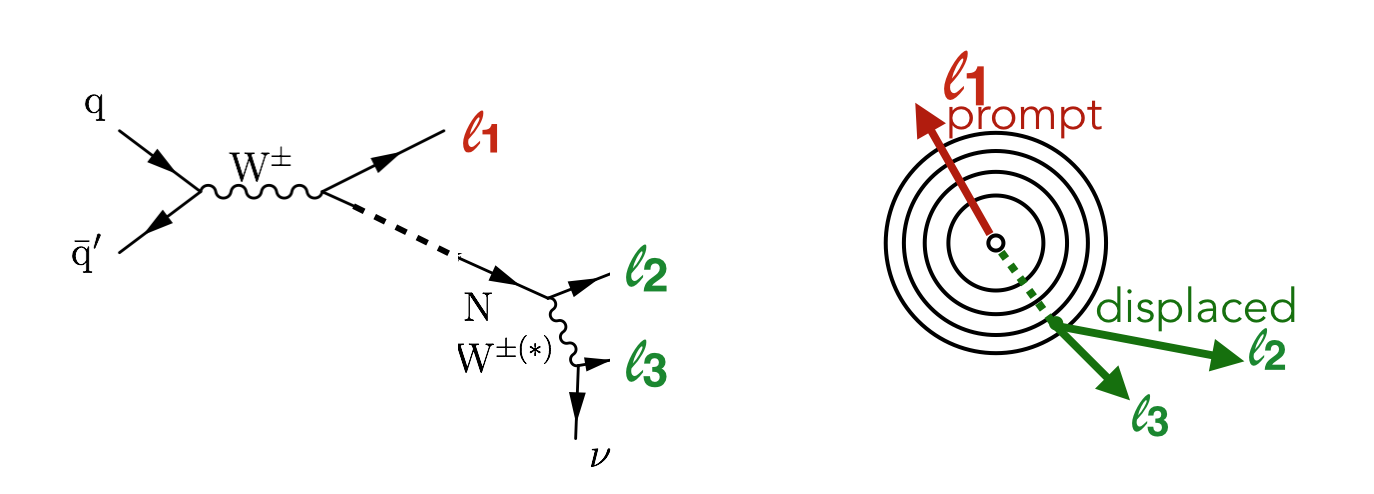
\includegraphics[width=0.85\textwidth]{Figures/c6/llsketch}
\caption{Diagram for the production of a long-lived HNL (left) with colors
  underlining the nomenclature adopted in the following
  sections. Prompt lepton referred to as \lone and two \displ leptons (\ltwo and \lthree). Didactic sketch on the right showing the usual signature with
 \lone back-to-back with respect to \ltwo and \lthree which form a SV.}
\label{fig:c6llsketch}
\end{figure}



Figure~\ref{fig:llfeatures} illustrates some
kinematic properties of the leptons in signal events, both at the
generator and reconstruction levels.\\
Given the low HNL masses considered in this analysis (\mhnl < 20\GeV),
\lone has the typical \pt spectrum expected for \PW decays, with a
Jacobian peak around 40\GeV,
while \ltwo and \lthree have very soft \pt spectra
(Figure~\ref{fig:llfeatures} (top-left)), invariant mass smaller than
\mhnl (Figure~\ref{fig:llfeatures} (top-right)), and a small opening angle
(Figure~\ref{fig:llfeatures} (bottom-left)).
In the absence of significant hadronic activity, \lone and \hnl are
typically separated by a large azimuthal angle
(Figure~\ref{fig:llfeatures} (bottom-right)).
These features, along with the possible displacement of \ltwo and
\lthree, can be used to identify the two leptons coming from the HNL
decay.

\begin{figure}[h!]
\centering
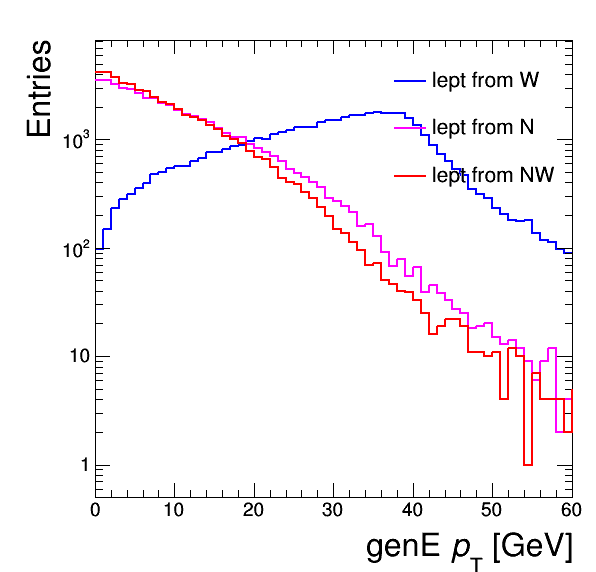
\includegraphics[width=.40\textwidth]{Figures/c6/selection/genE_vs_pt_sortby_prov_m4.png}
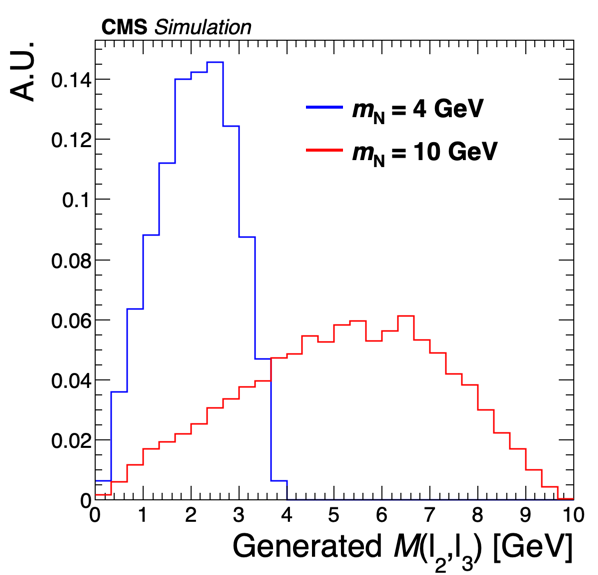
\includegraphics[width=.40\textwidth]{Figures/c6/selection/l2l3_mass_gen.png}\\
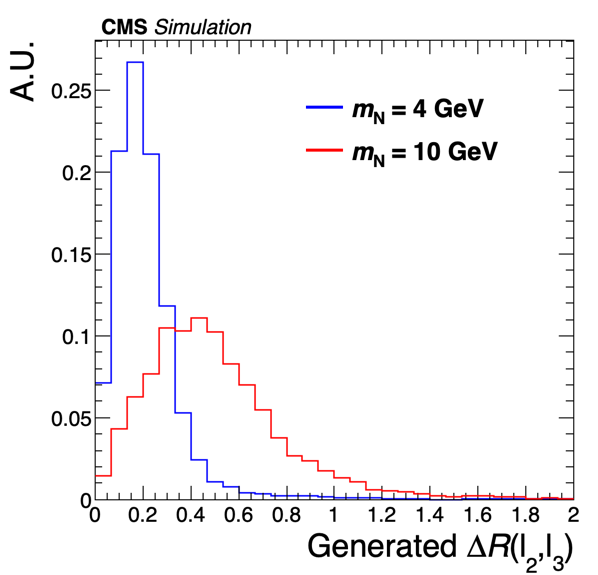
\includegraphics[width=.40\textwidth]{Figures/c6/selection/l2l3_dR_gen.png}
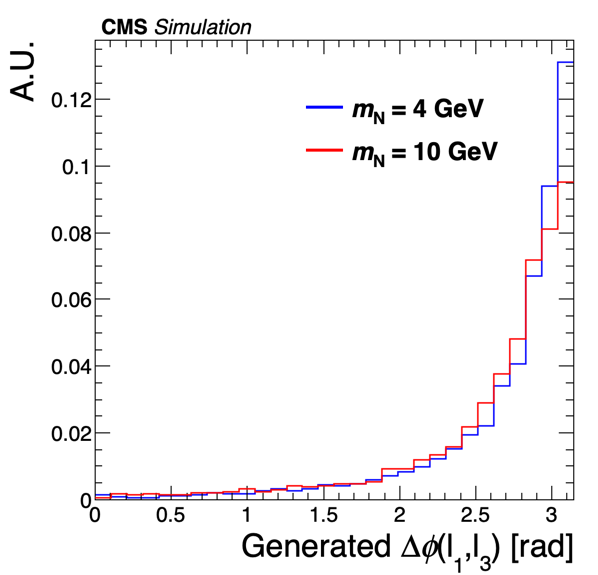
\includegraphics[width=.40\textwidth]{Figures/c6/selection/l1l3_dPhi_gen.png}
  \caption{For the HNL scenario:HNL of mass
    $\mhnl=4$\GeV and $\mixpar=10^{-4}$. Top left, generated lepton \pt, separately
    for \lone (``from \PW''), \ltwo (``from \hnl''), and \lthree
    (``from $\hnl\PW$'').
Top right, invariant mass of \ltwo
    and \lthree 
    at generator level.
Bottom left, \DR\ between \ltwo 
    and \lthree.
Bottom right, \Dphi between \lone
    and \lthree. \dani}
  \label{fig:llfeatures}
\end{figure}

\subsection{HNL candidate selection}
As shown in Tables~\ref{tab:electronSelection} and
\ref{tab:muonSelection},
the displacement of \ltwo and \lthree is requested by imposing a
minimum \absdxy cut of 0.1~mm to the reconstructed leptons.
Given the rapid variation of the \hnl displacement with \mhnl and
\mixpar, this preliminary displacement requirement must be rather
mild, and does not resolve completely possible ambiguities between
prompt and \displ reconstructed leptons.

Other than the two leptons from the HNL decay, additional
leptons---real or misidentified---may satisfy the \absdxy requirements
and pass the \displ-lepton selection. In this case, criteria must
be put in place to resolve the ambiguities and correctly identify the
two leptons from the HNL decay.
To this purpose, variables such as the invariant mass of \ltwo and
\lthree, \mtwol, and the \DR\ separation between \ltwo and \lthree, \DRtwol, are found to be
effective, and with similar performances.
Therefore, the three leptons from HNL decay are identified as follows.
Among all the leptons that pass the prompt selection of
Tables~\ref{tab:electronSelection} and \ref{tab:muonSelection}, the one
with highest \pt is chosen as \lone and it is not considered anymore for the selection of \ltwo and \lthree.
Among all the selected \displ leptons, the two leptons of any
flavor with the largest di-lepton \pt (vectorial sum of $p_{T_{\ltwo}}$
and $p_{T_{\lthree}}$) and opposite charge are selected
as \ltwo and \lthree,
($\Pe^\pm\Pe^\mp$, $\Pe^\pm\PGm^\mp$, $\PGm^\pm\PGm^\mp$).
If there is no opposite-charge \displ leptons pair, the
event is rejected. This reduces background processes with
mis-identified leptons, while retaining almost full efficiency for the
signal. In the following, we will label \ltwo (\lthree) the lepton in
the pair with higher (lower) \pt.\\
This selection strategy correctly identifies the one prompt and two
\displ leptons in more than 99\% of signal events (99.9\% of
signal events that pass the full analysis selection, described in
Section~\ref{sec:llbaselinesel}).

\subsubsection{Secondary vertex fit}

Once \ltwo and \lthree have been identified, we can reconstruct their
common vertex of origin, \ie the decay vertex of the HNL. \\
For the SV reconstruction the procedure described in Section~\ref{sec:c2sv} is used.
The fitted SV estimates the production vertex of \ltwo and \lthree.

\subsection{Event kinematics and baseline selection}
\label{sec:llbaselinesel}

Starting from all events with one prompt lepton and two \displ
leptons forming a SV, the kinematic properties and particle content of
typical HNL signal events are used to suppress the background
contributions (more details in the following Section~\ref{sec:llbackground}).

The baseline selection includes the following requirements, summarized
in Table~\ref{tab:baselinesel}. Please
consider Figure~\ref{fig:c6llsketch} as reference for lepton
nomenclature. The distributions of all the variables used for the
selection are shown in Figure~\ref{fig:selection_electrons}.
{\footnotesize
\begin{table}[h!]
  \centering
  \caption{\label{tab:baselinesel} Baseline selection requirements
    applied to all data sets.}
  \begin{tabular}{l|l}
    \hline
    Variable     & Requirement       \\
    \hline
    \hline
       \DRtwol      & $<1$              \\
    \minDphi     & $>1$ rad          \\
    \mlll     & $\in [50,80]$\GeV \\
    N. \PQb & $=0$              \\
    \pt (\ltwo $+$ \lthree) & $> 15$\GeV             \\
    \costheta    & $>0.99$            \\
    $p_{SV}$ & $> 0.001$              \\
    $S(\Delta_{2D})$& $>20$              \\ 
    resonance vetoes & \checkmark       \\
    \hline
    \hline
  \end{tabular}
\end{table}
}

As explained above, \ltwo and \lthree are expected to have small
opening angle, given the small mass and relatively large momentum of
the HNL. As can be seen in
Figure.~\ref{fig:selection_electrons} (top-left),
the variable \DRtwol discriminates the signal from all background
processes. To retain high signal efficiency and reduce backgrounds
where two leptons are relatively separated from each other, we select events with
$\boldsymbol{\DRtwol<1}$.
\vspace{2mm}

In the absence of energetic jets in signal events, \lone is expected
to recoil at a large angle in the transverse plane from the HNL, and
thus from \ltwo and \lthree. Since both $\Dphi(\lone,\ltwo)$ and
$\Dphi(\lone,\lthree)$ are large and close in value (which may not be
true for other processes with two uncorrelated nonprompt leptons), we
apply a cut on the smaller of the two angles,
$\boldsymbol{\minDphi>1\,\mathrm{rad}}$. \\

The invariant mass of the three charged leptons \mlll, \mthreel, is limited
by the mass of the on-shell \PW boson. Given the relatively low
momentum carried away by the neutrino, \mlll tends to peak just
below the \PW mass, with a steep fall above 80\GeV and a larger tail
at lower masses. We select
events with $\boldsymbol{\mlll}$ values \textbf{between 50 and 80\GeV}. This requirement
proves particularly effective against the Z$\gamma^{(\ast)}$ background, where the
photon radiated by one of the leptons from the \PZ decay undergoes an
asymmetric conversion: one of the leptons receives most of the \PGg
momentum, while the other is too soft to be detected or
identified. Such events manifest themselves as a peak at about 91\GeV in the \mthreel
spectrum. \\

Events with a b jet (see Section~\ref{sec:object}) with \pt greater
than 25\GeV are rejected, in order to substantially reduce the
background from the top processes.\\

The vector sum of the momenta of \ltwo, \lthree, and the neutrino
corresponds to the momentum of the HNL, and points back exactly to the
PV. Unfortunately the total momentum of the neutrino is unknown, and
its transverse momentum, estimated by \ptmiss, has limited resolution.
The decay products of the HNL, however, are emitted at small opening
angles with respect to the HNL direction. We can thus expect the
vector sum of the \ltwo and \lthree momenta to follow closely, though
not exactly, the direction of the
HNL. Figure~\ref{fig:selection_electrons} shows a distribution of the cosine of the angle between the SV
position, which estimates the direction of flight of the HNL before
decaying, and the vector sum of the \ltwo and \lthree momenta
(``back-pointing angle''):
$\costheta = \vec{r}_{\mathrm{SV}}\cdot\vec{p}_{\mathrm{\ltwothree}}/
\left(|\vec{r}_{\mathrm{SV}}||\vec{p}_{\mathrm{\ltwothree}}|\right)$.
As expected, the signal events peak at values very close to 1,
$\boldsymbol{\costheta > 0.99}$.
Processes with two uncorrelated nonprompt leptons should exhibit a
flat \costheta distribution. The requirement on \DRtwol, however,
selects events with two relatively close-by leptons, therefore the
vector sum of the \pt of the two displaced leptons makes a small angle
with the vector drawn from the PV to SV. In principle this is a
genuine property of the boosted displaced HNL, however the angular
cuts on the two leptons biases the background to have small angle as
well. For this reason, all
background processes exhibit a peaking structure, randomly at $-1$ or
$+1$.\\

The quality of the secondary vertex ($\boldsymbol{ p_{SV}}$) necessarily correlates with the precision of the trajectories from \ltwo and \lthree as well as how close they are at the intersection point. It is represented as a probability based on the maximum likelihood fit from the kinematic vertex fitter. One can observe that for low probability values, the background dominates. This motivates a requirement of the \textbf{probability to be larger than 0.001}. \\

The quality of the SV fit is used as well as discriminating variable against random vertices. The significance of the distance between PV and SV, $\boldsymbol{ S(\Delta_{2D})}$ is shown in Figure~\ref{fig:selection_electrons}. The requirement of the \textbf{significance to be larger than 20} is applied.\\

The dilepton (\ltwo, \lthree) transverse momentum  is required to be
larger than 15\GeV, since the low-\pt region is heavily dominated by
the nonprompt lepton background.
The dilepton mass \mtwol distribution has an upper cut that
corresponds to the largest mass among all the considered signal
samples. Due to the presence of the neutrino in the final state, the
mass is always lower than the HNL mass.\\

In addition to the selections mentioned above, numerous dilepton
resonances within the search
 region are removed.
In case of \ltwo and \lthree having the same flavor and opposite
charges and with the transverse position of the dilepton vertex
$\Deltwod<1.5$\cm, the following resonance masses (\mtwol) are
removed: 
\JPsi $(3.10 \pm 0.08$\GeV), \Pgy $(3.69 \pm 0.08$\GeV), $\omega$
$(0.78 \pm 0.08$\GeV), and $\phi$ $(1.02 \pm 0.08$\GeV).
In case \lone and \ltwo/\lthree have the same flavor and opposite
charges, events are removed if \mlonetwo or \mlonethree are in the
ranges listed above, or consistent with other higher-mass resonances,
including \PgUa $(9.46 \pm 0.08$\GeV), \PgUb $(10.02 \pm 0.08$\GeV),
\PgUc $(10.36 \pm 0.08$\GeV), and \PZ $(91.19 \pm 10.00$\GeV).
 \begin{figure}[h]
\centering
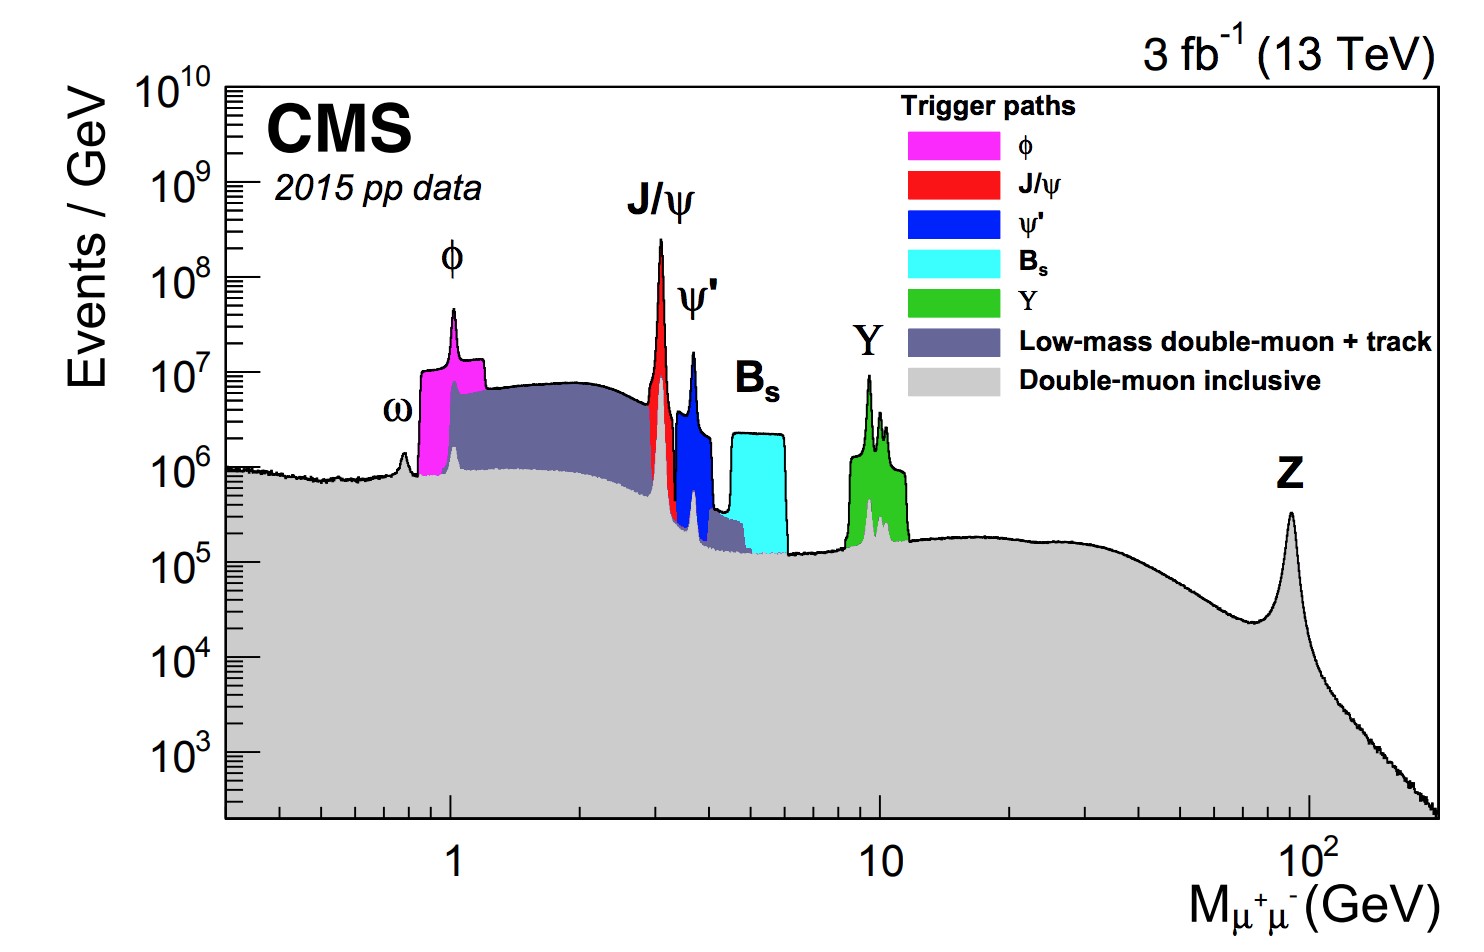
\includegraphics[clip,trim=1.2cm 0.1cm 0.8cm 0.3cm, width=.70\textwidth]{Figures/c2/dimuon}
\caption{The dimuon invariant mass distribution showing dilepton resonances~\cite{Sirunyan_2018_muon}.}
\label{fig:c6dimuon}
\end{figure}

\begin{center}
\framebox{
       \parbox{.95\textwidth}{
{\footnotesize
The convention for the legends in all following plots in Chapter~\ref{Chapter6} backgrounds
will be grouped into macro-categories of histograms as follows.
When there are only MC predictions:
\begin{itemize}
\setlength\itemsep{-0.2em}
\item {\color{gray}MC nonprompt DF:} processes that give rise to two nonprompt
  leptons, such as \PW + jets, \ttbar + jets, single-top. To be defined as DF it has to be defined "double-fake" according to the definition in Section~\ref{sec:llbackground};
\item {\color{gray}MC nonprompt SF:} processes that give rise to one or two nonprompt
  leptons, such as \PW + jets, \ttbar + jets, single-top and DY+ jets. To be defined as SF it has to be defined "single-fake" according to the definition in Section~\ref{sec:llbackground};
\item {\color{gray}Conversions:}  processes with photon conversions, such as Z$\PGg$ and W$\PGg$;
\item {\color{gray}$\PZ\PGg^{\ast}$:} we consider DY events with prompt leptons;
\item {\color{gray}Other:} processes like diboson and triboson.
\end{itemize}
When there are both MC and data-driven predictions:
\begin{itemize}
\setlength\itemsep{-0.2em}
\item {\color{gray}Nonprompt DF/SF:} data-driven predictions that are explained in Section~\ref{sec:llbackground};
\item {\color{gray}Conversions:}  processes with photon conversion, like Z$\PGg$ and W$\PGg$, and DY;
\item {\color{gray}Other:} processes like diboson and triboson.
\end{itemize}
}
}
}
\end{center}

\begin{figure}[h]
\centering
  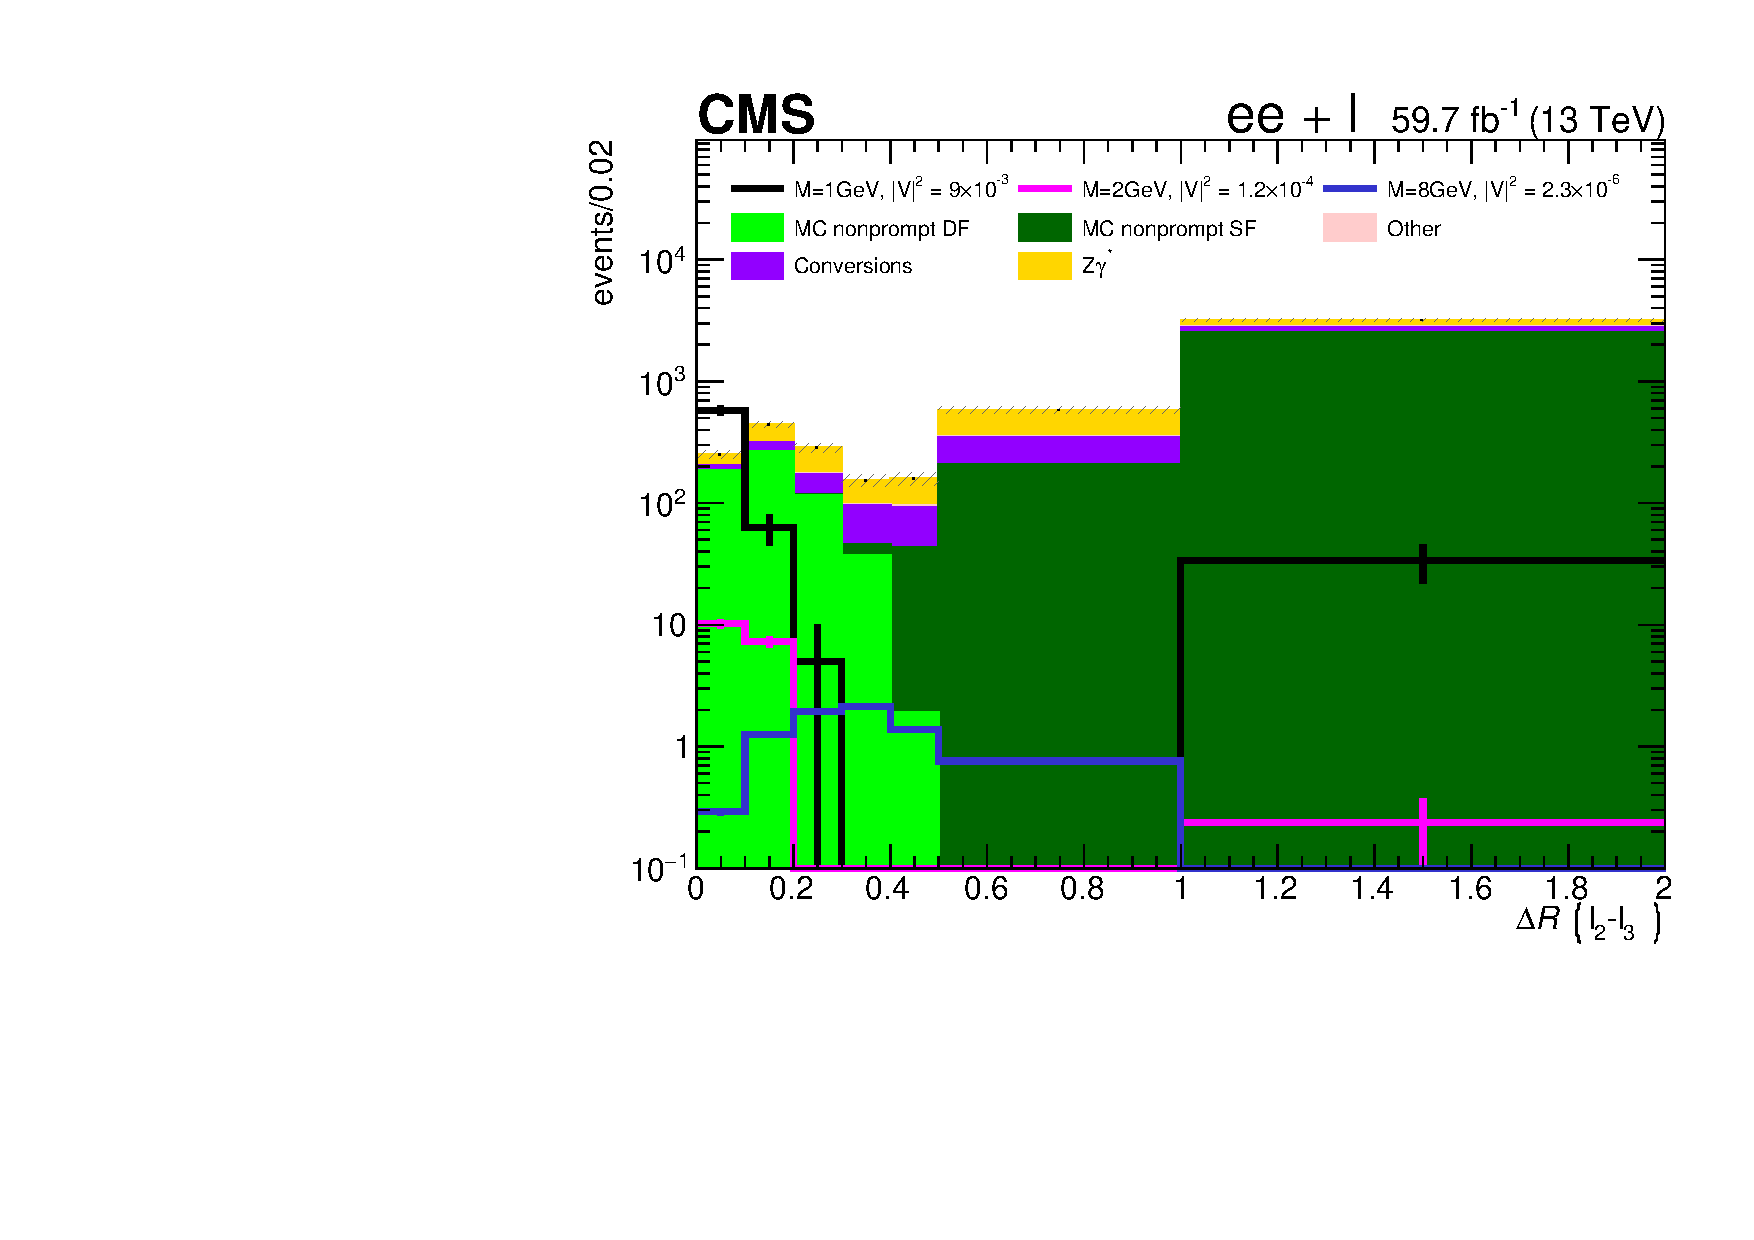
\includegraphics[clip,trim=0.9cm 0.7cm 0.7cm 0.6cm,width=.35\textwidth]{Figures/c6/selection/18/e_DeltaR_l2_l3__0.pdf}
  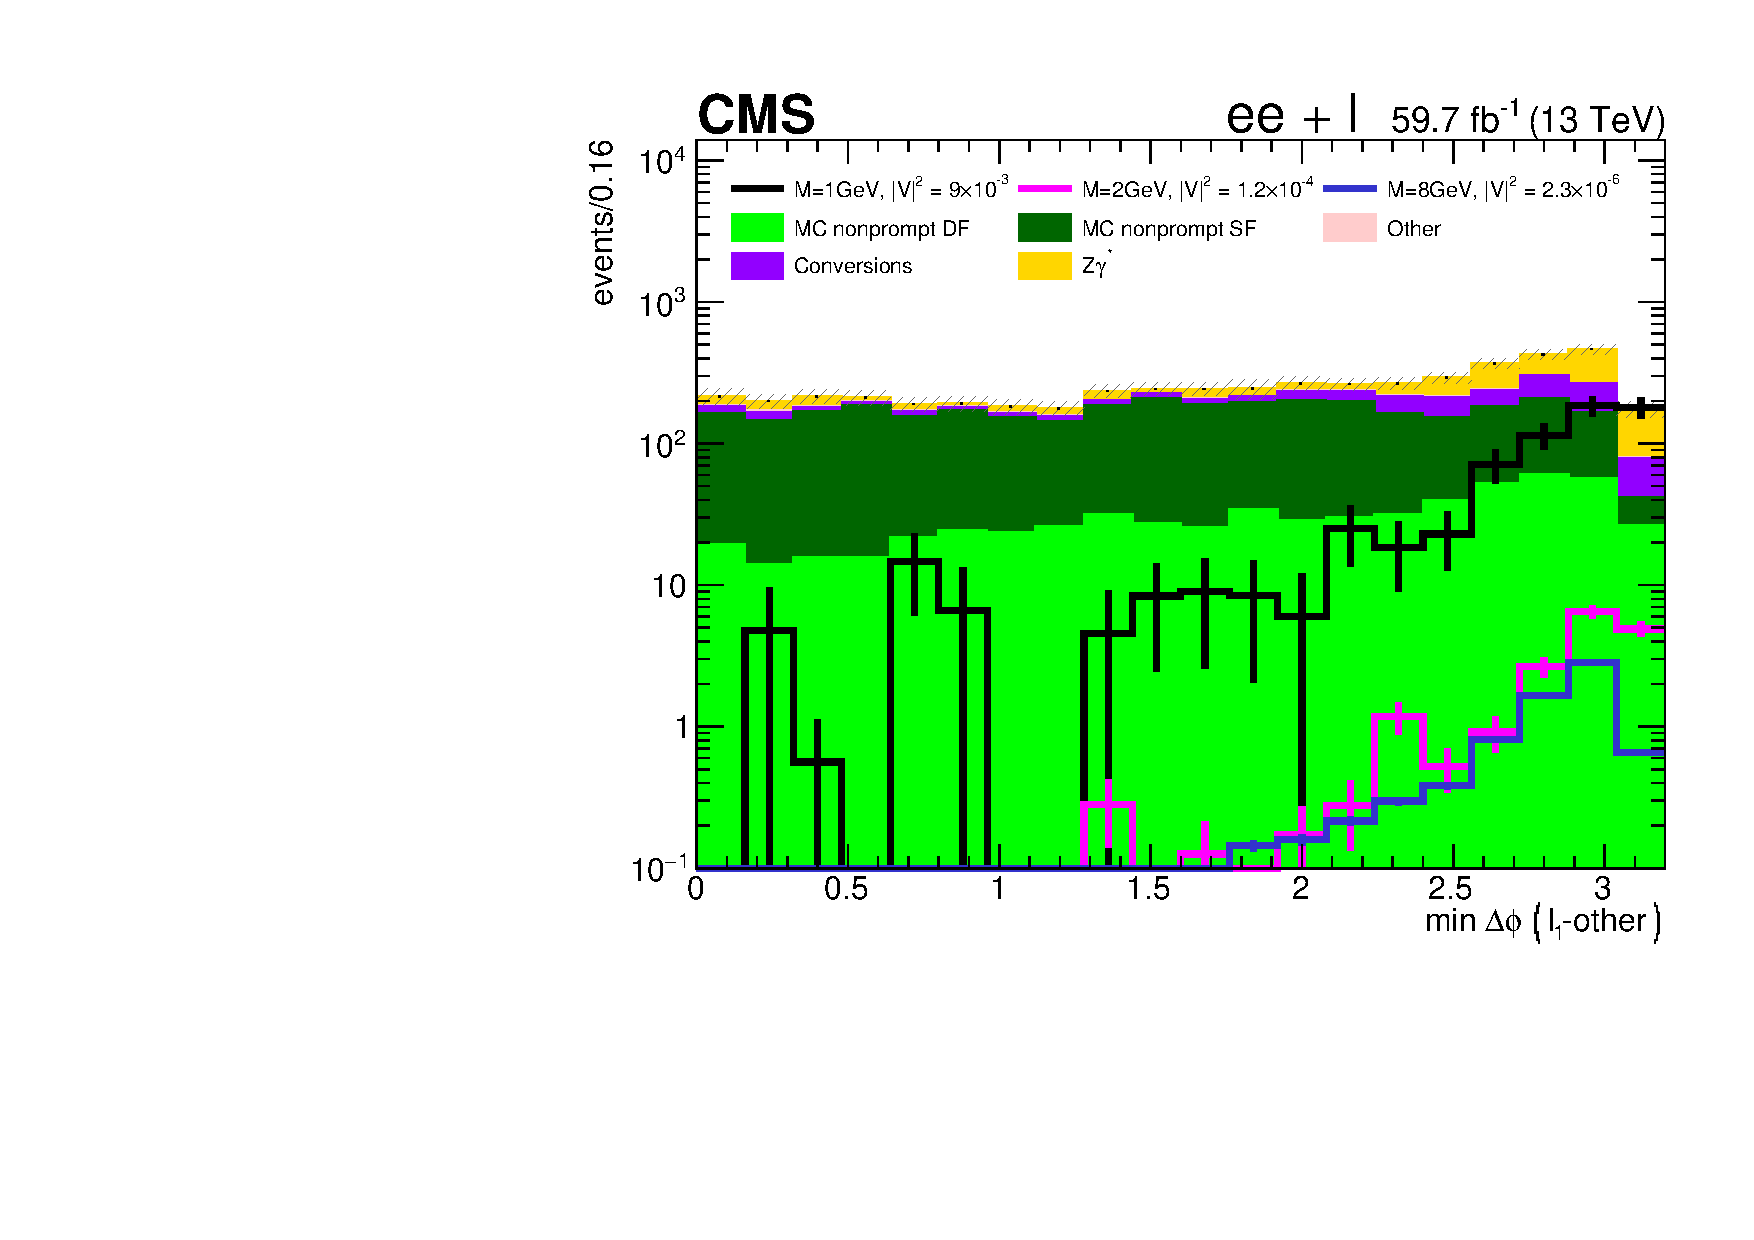
\includegraphics[clip,trim=0.9cm 0.7cm 0.7cm 0.6cm,width=.35\textwidth]{Figures/c6/selection/18/e_minDeltaphil1_other__0.pdf}\\
  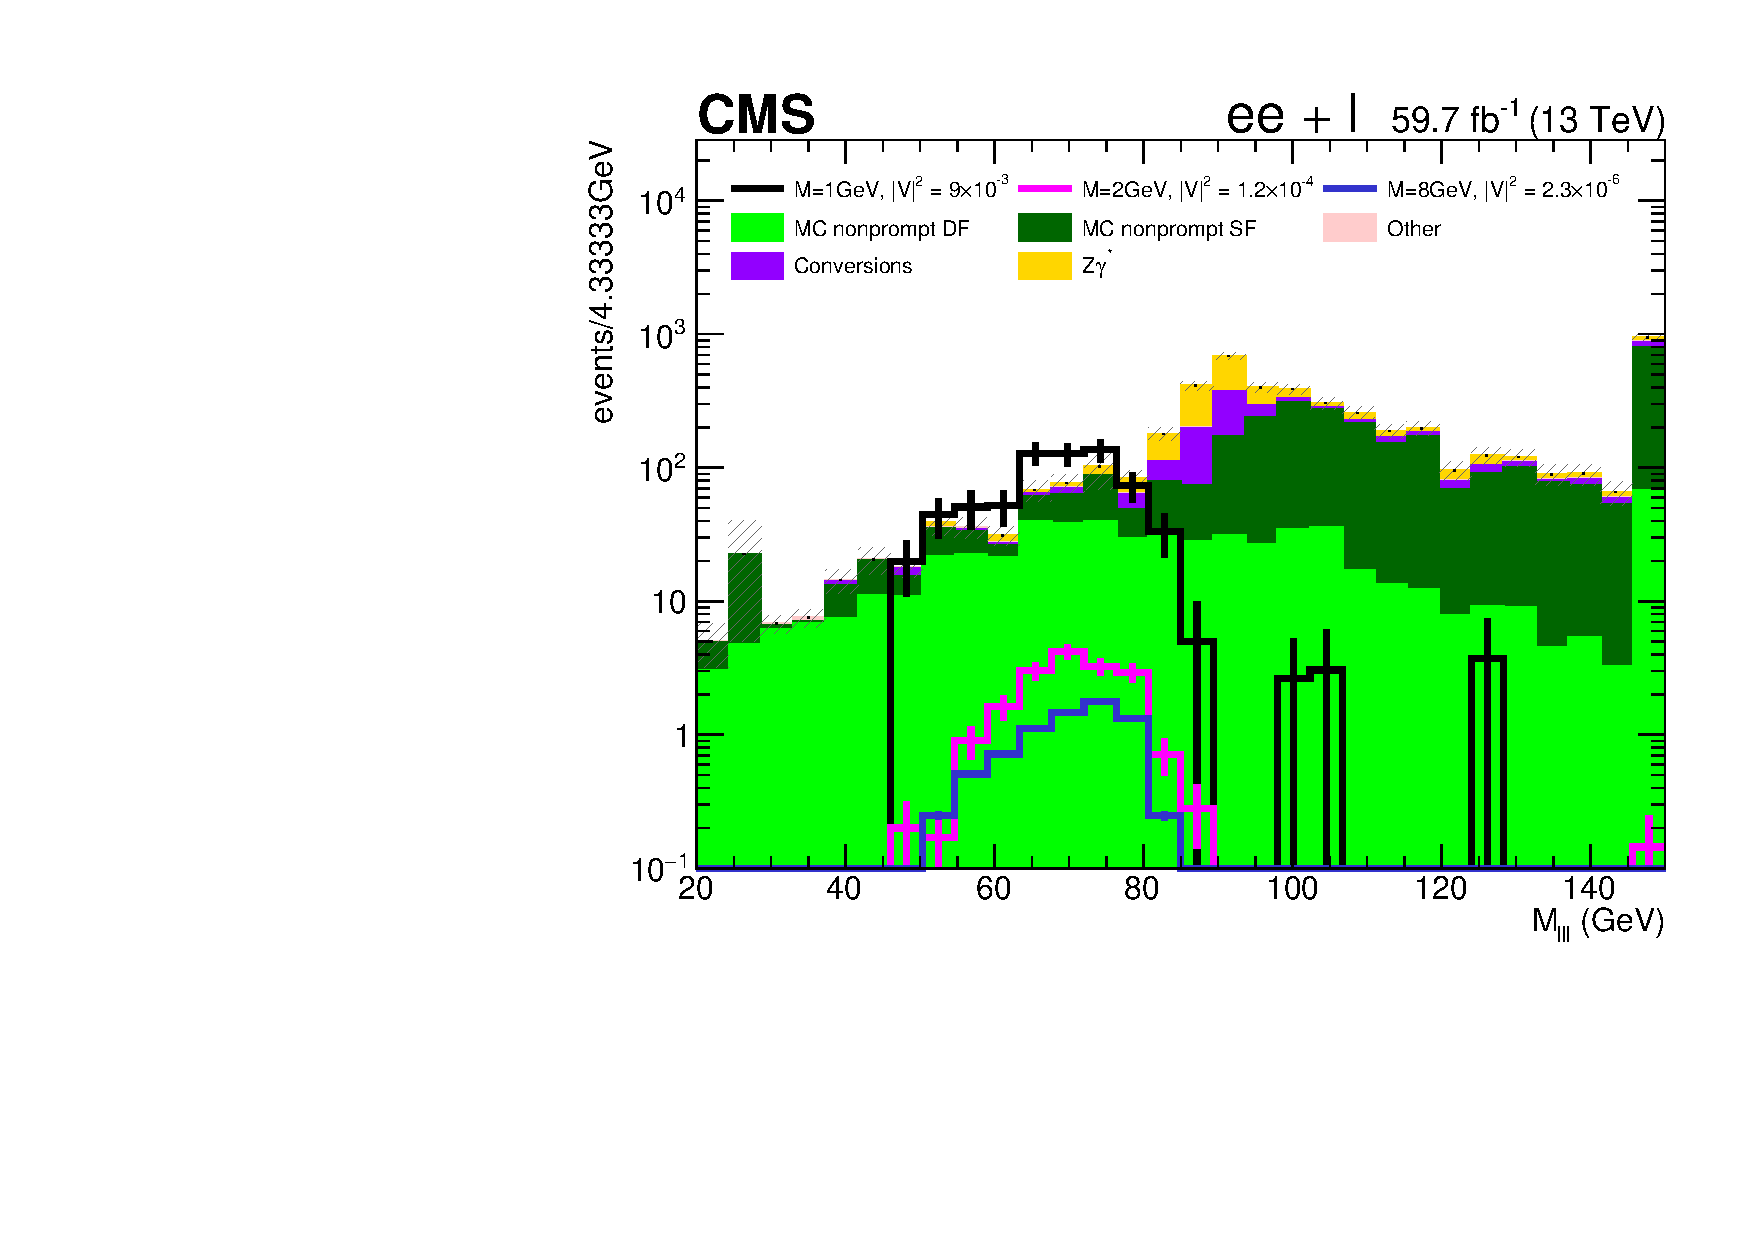
\includegraphics[clip,trim=0.9cm 0.7cm 0.7cm 0.6cm,width=.35\textwidth]{Figures/c6/selection/18/e_M_lll__0.pdf}
  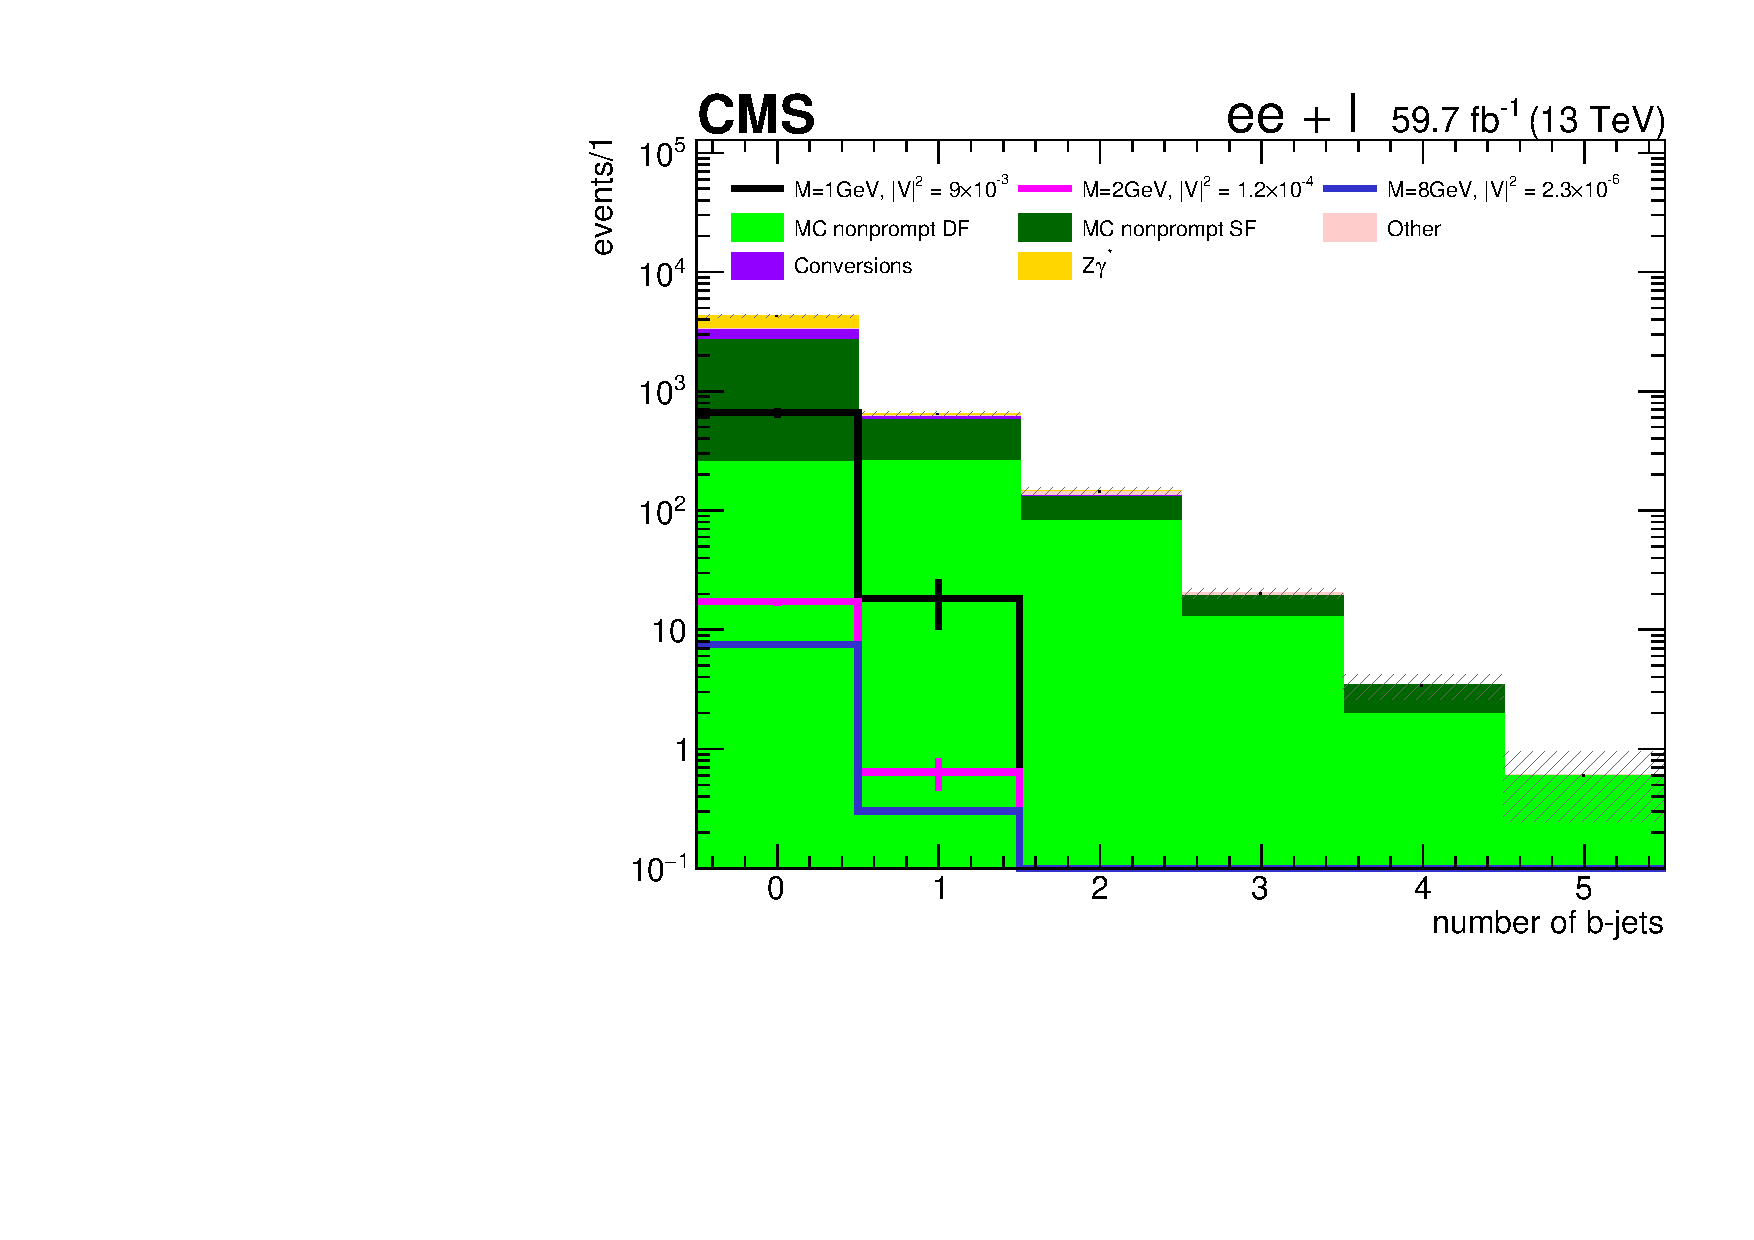
\includegraphics[clip,trim=0.9cm 0.7cm 0.6cm
  1.0cm,width=.35\textwidth]{Figures/c6/selection/18/e_numberofb_jets__0.pdf}\\
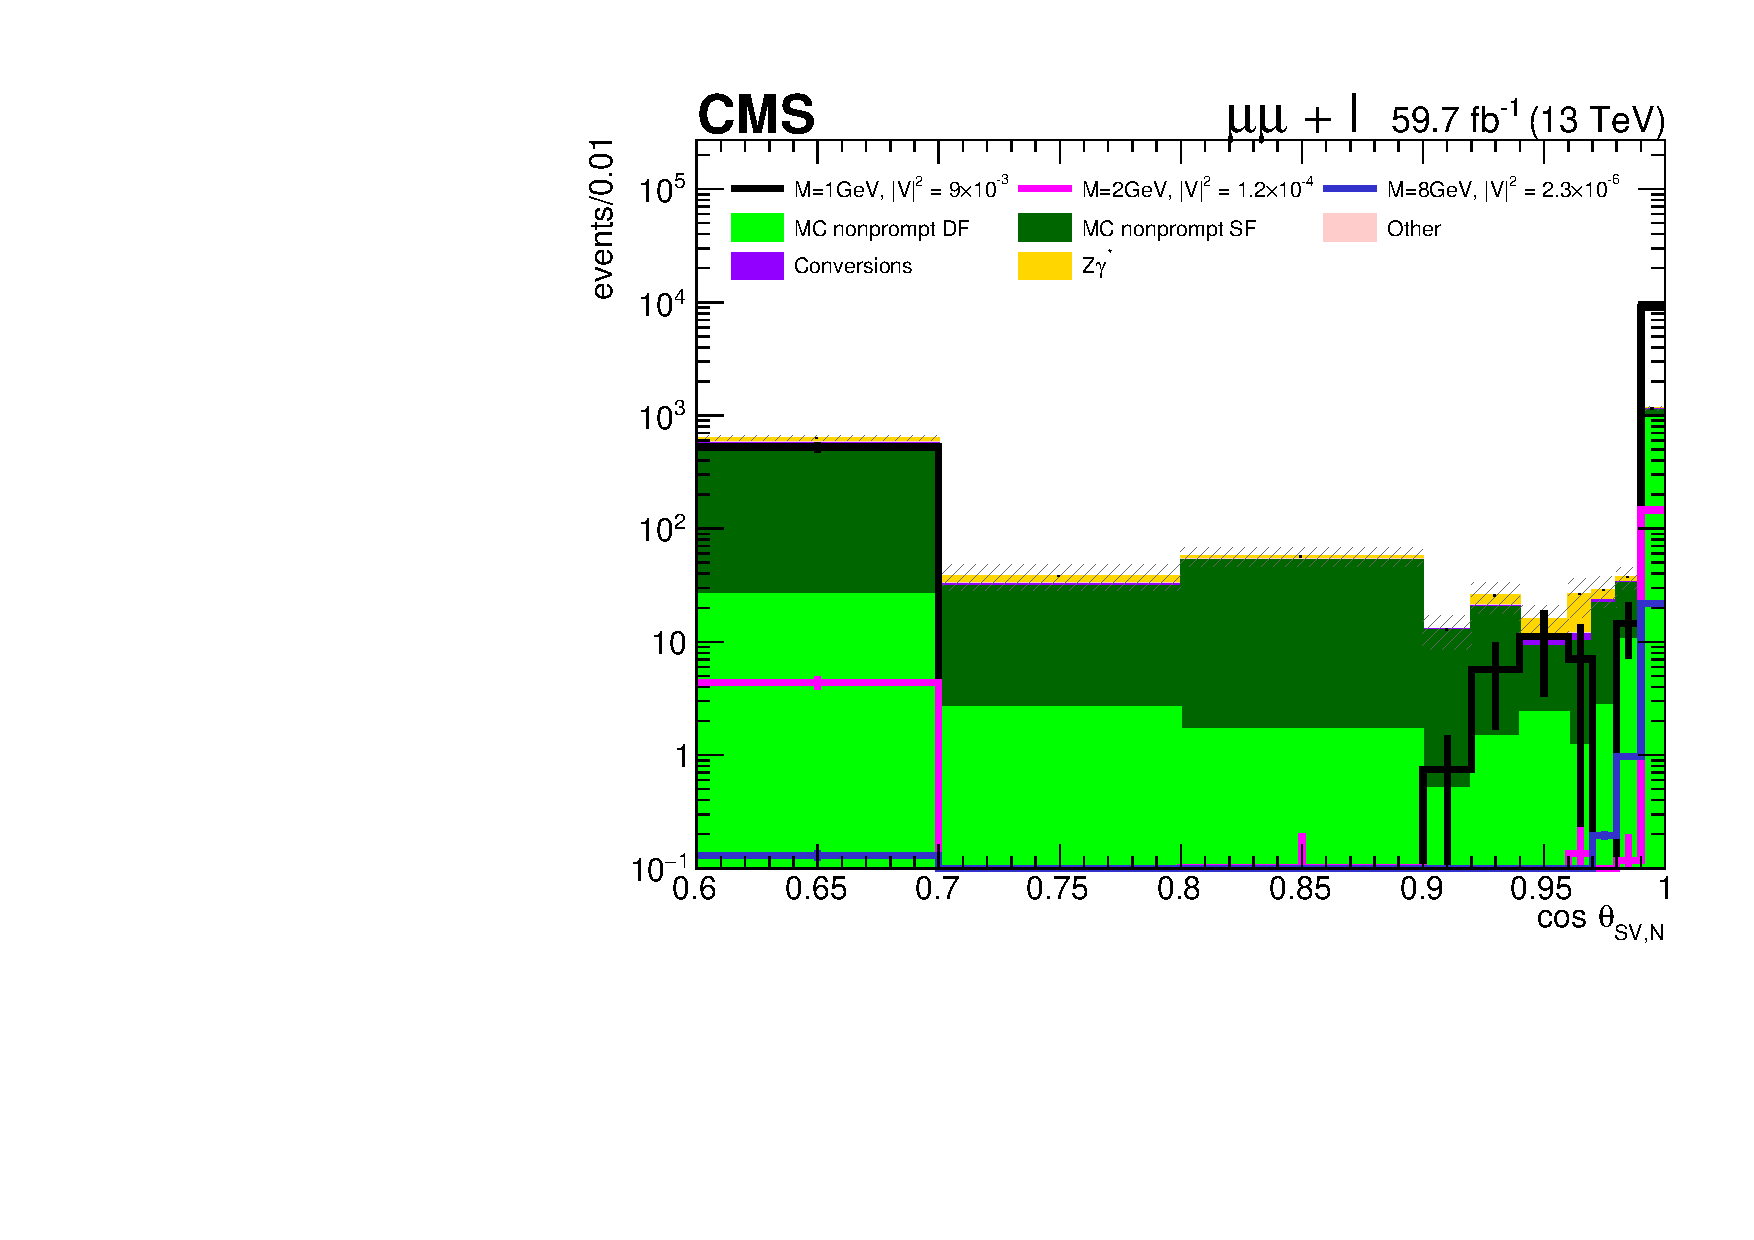
\includegraphics[clip,trim=0.9cm 0.7cm 0.7cm 0.6cm,width=.35\textwidth]{Figures/c6/selection/18/mu_cosSVposl2_l3dir__0.pdf}
  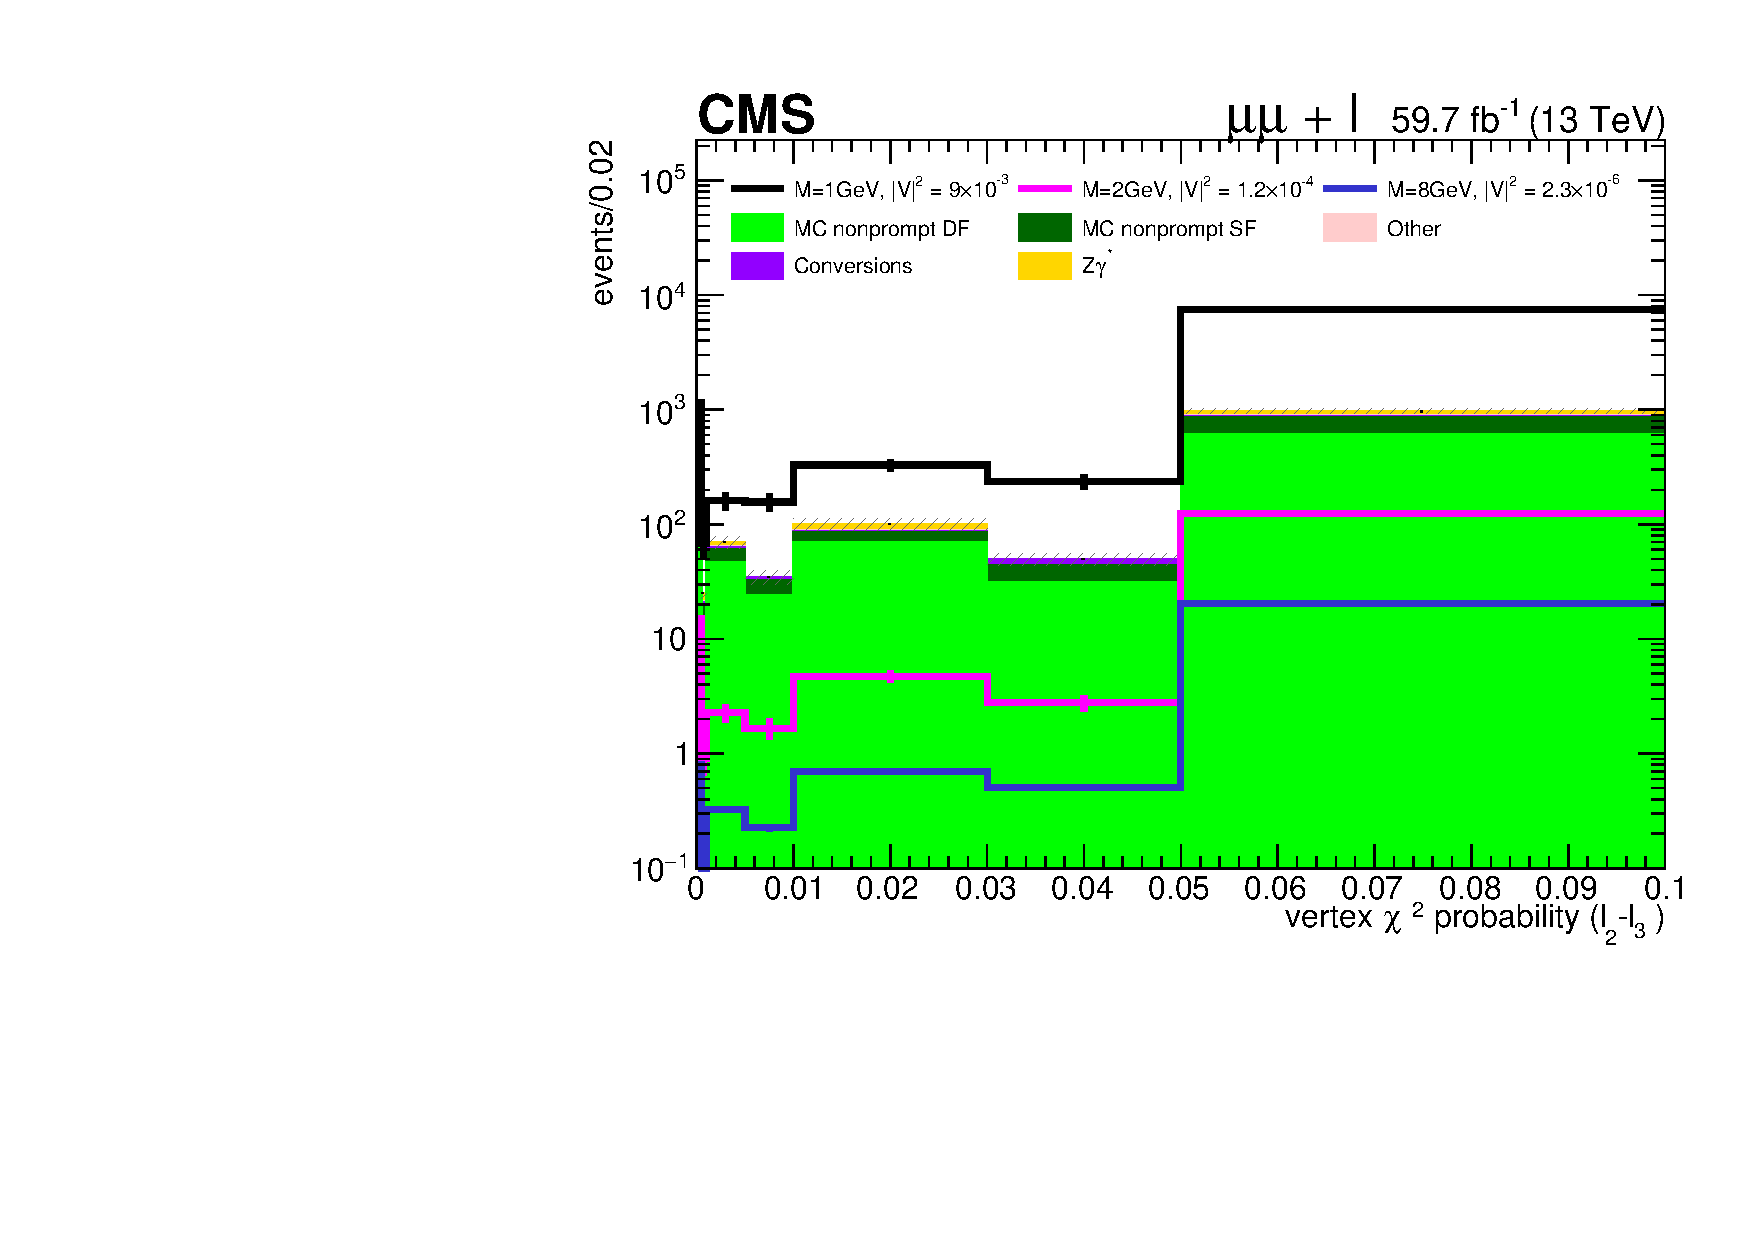
\includegraphics[clip,trim=0.9cm 0.7cm 0.7cm 0.6cm,width=.35\textwidth]{Figures/c6/selection/18/mu_vertexchi2_probabilityl2_l3__0.pdf}\\
  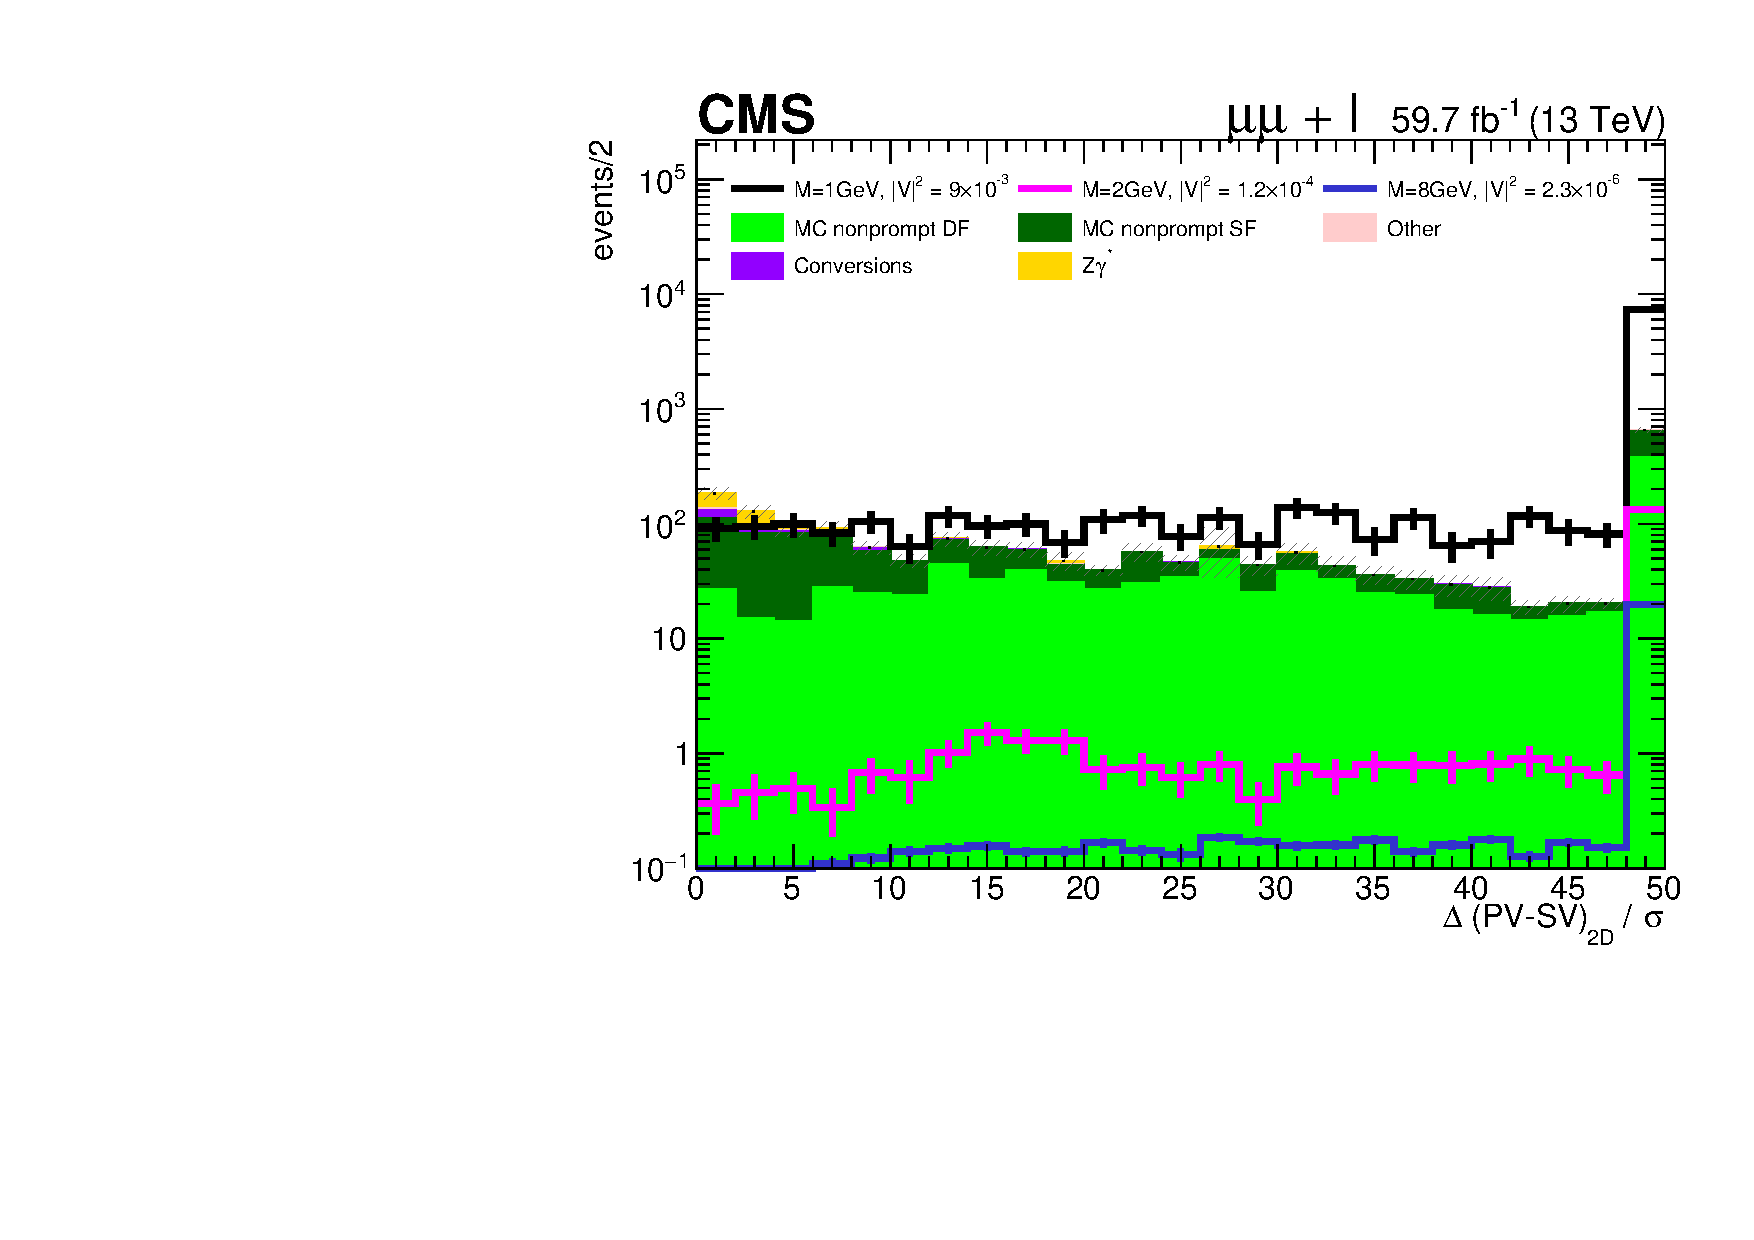
\includegraphics[clip,trim=0.9cm 0.7cm 0.7cm 0.6cm,width=.35\textwidth]{Figures/c6/selection/18/mu_sigmaDeltaPV_SV_2D__0.pdf}
  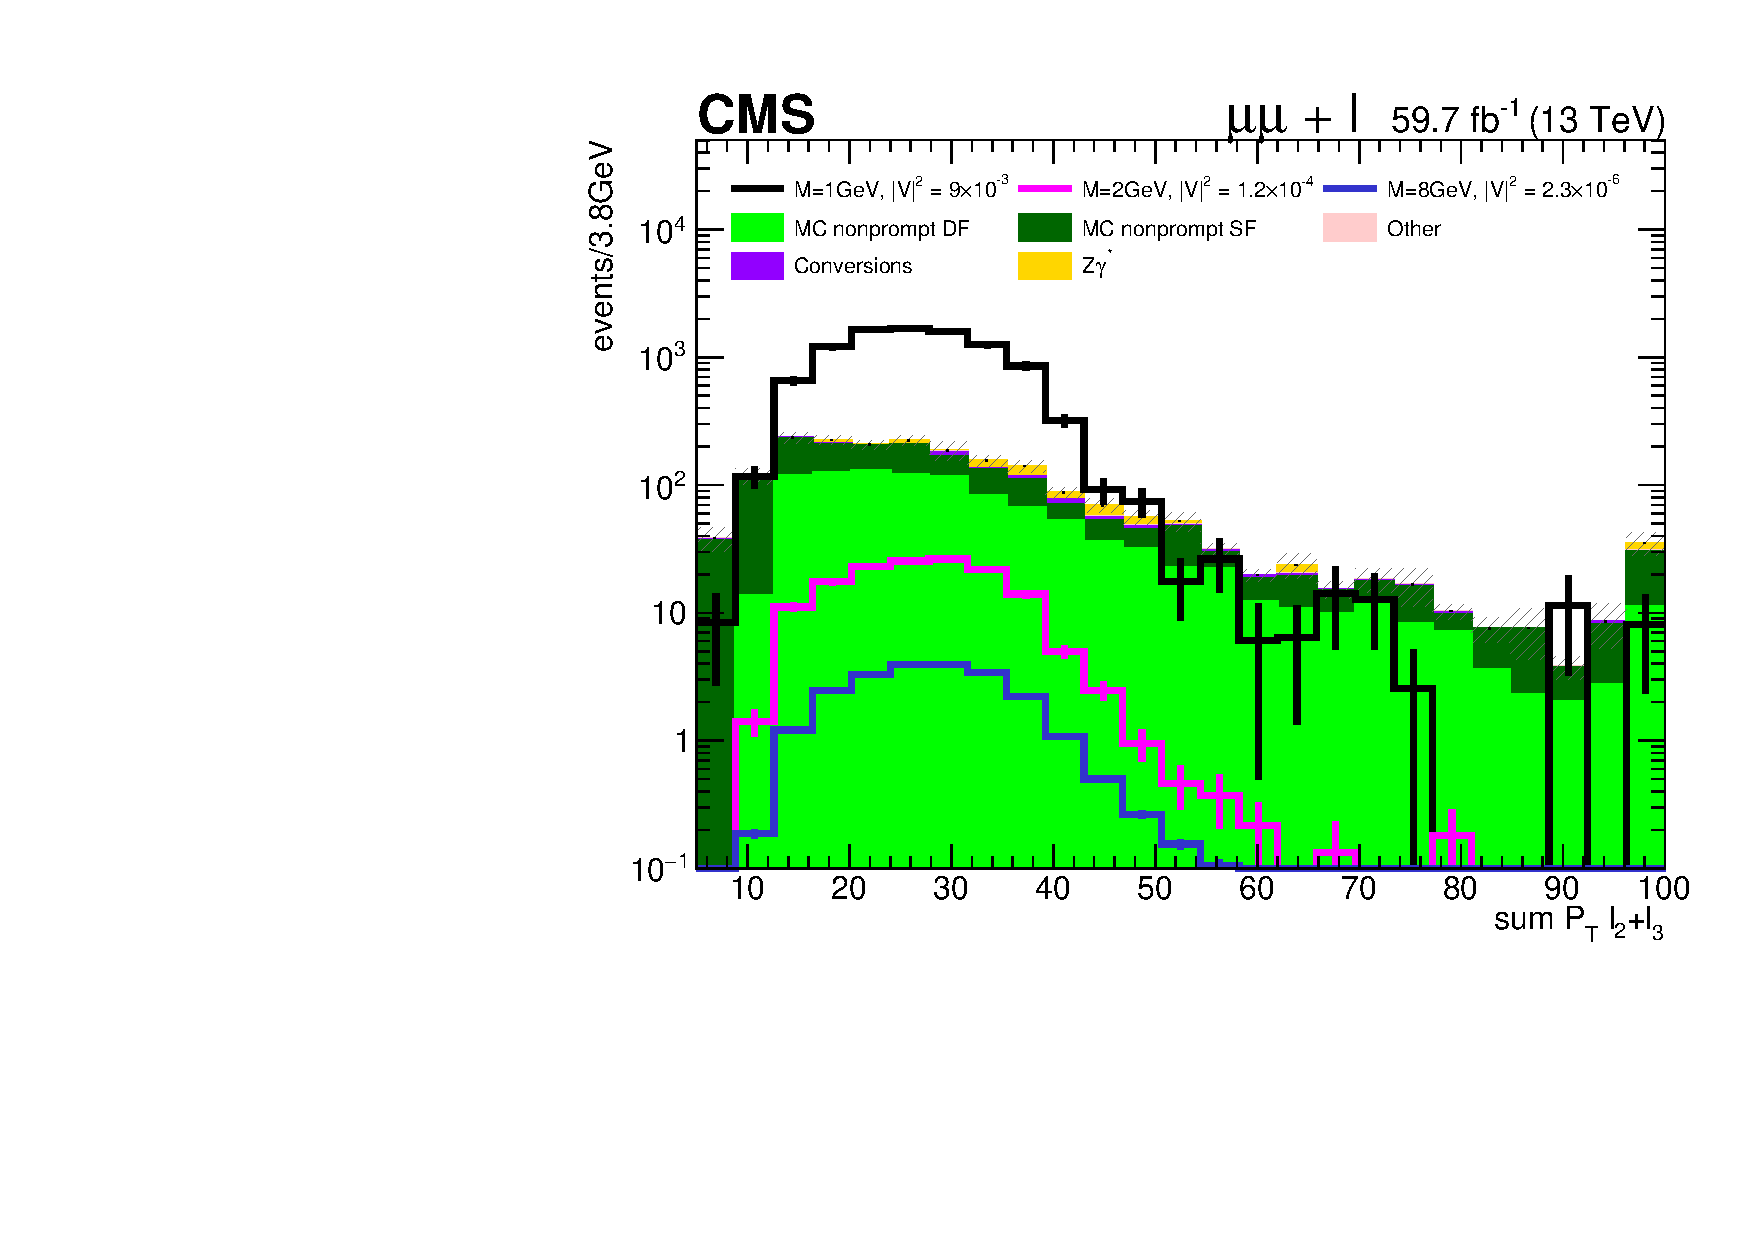
\includegraphics[clip,trim=0.9cm 0.7cm 0.7cm 0.6cm,width=.35\textwidth]{Figures/c6/selection/18/mu_sum_Pt_L2L3__0.pdf}
  \caption{Distributions of the event selection's variables listed in
    Table~\ref{tab:baselinesel}. Simulated backgrounds (shaded histograms, stacked),
    using the 2018 MC samples, 
    after the selection of the three leptons \lone, \ltwo, and \lthree,
    in \eex final states for the top 4 plots and \mmx final states for
    the 4 bottom plots.
    Signal models for different values of \mhnl and \mixpar are shown
    as empty histograms.}
  \label{fig:selection_electrons}
\end{figure}


\clearpage
Figures~\ref{fig:cutflow1} and~\ref{fig:cutflow2} are a summary view of the entire selection
step by step showing two different kinds of "cutflow". The
first set, Figure~\ref{fig:cutflow1}, is the classic cutflow where each
bin displays the number of remaining events after each selection and it goes in a
"cascade" way (one after the other). The second one,
Figure~\ref{fig:cutflow2}, is a $N-1$ plot where each bin has the number
of events when that particular selection is not applied; in this way it is
possible to appreciate which is the real impact of each selection no matter
its arbitrary position in the event selection list. \\
As it is seen in Figure~\ref{fig:cutflow2}, the most effective
background rejection is achieved with the \mthreel selection. In
particular, it is effective in \eex final states as it rejects DY events
where at least one electron comes from conversion. In such events,
\mthreel values are in the region of $M_{\PZ}$ which remains outside the
[50-80]\GeV signal region.

\begin{figure}[h!]
\centering
  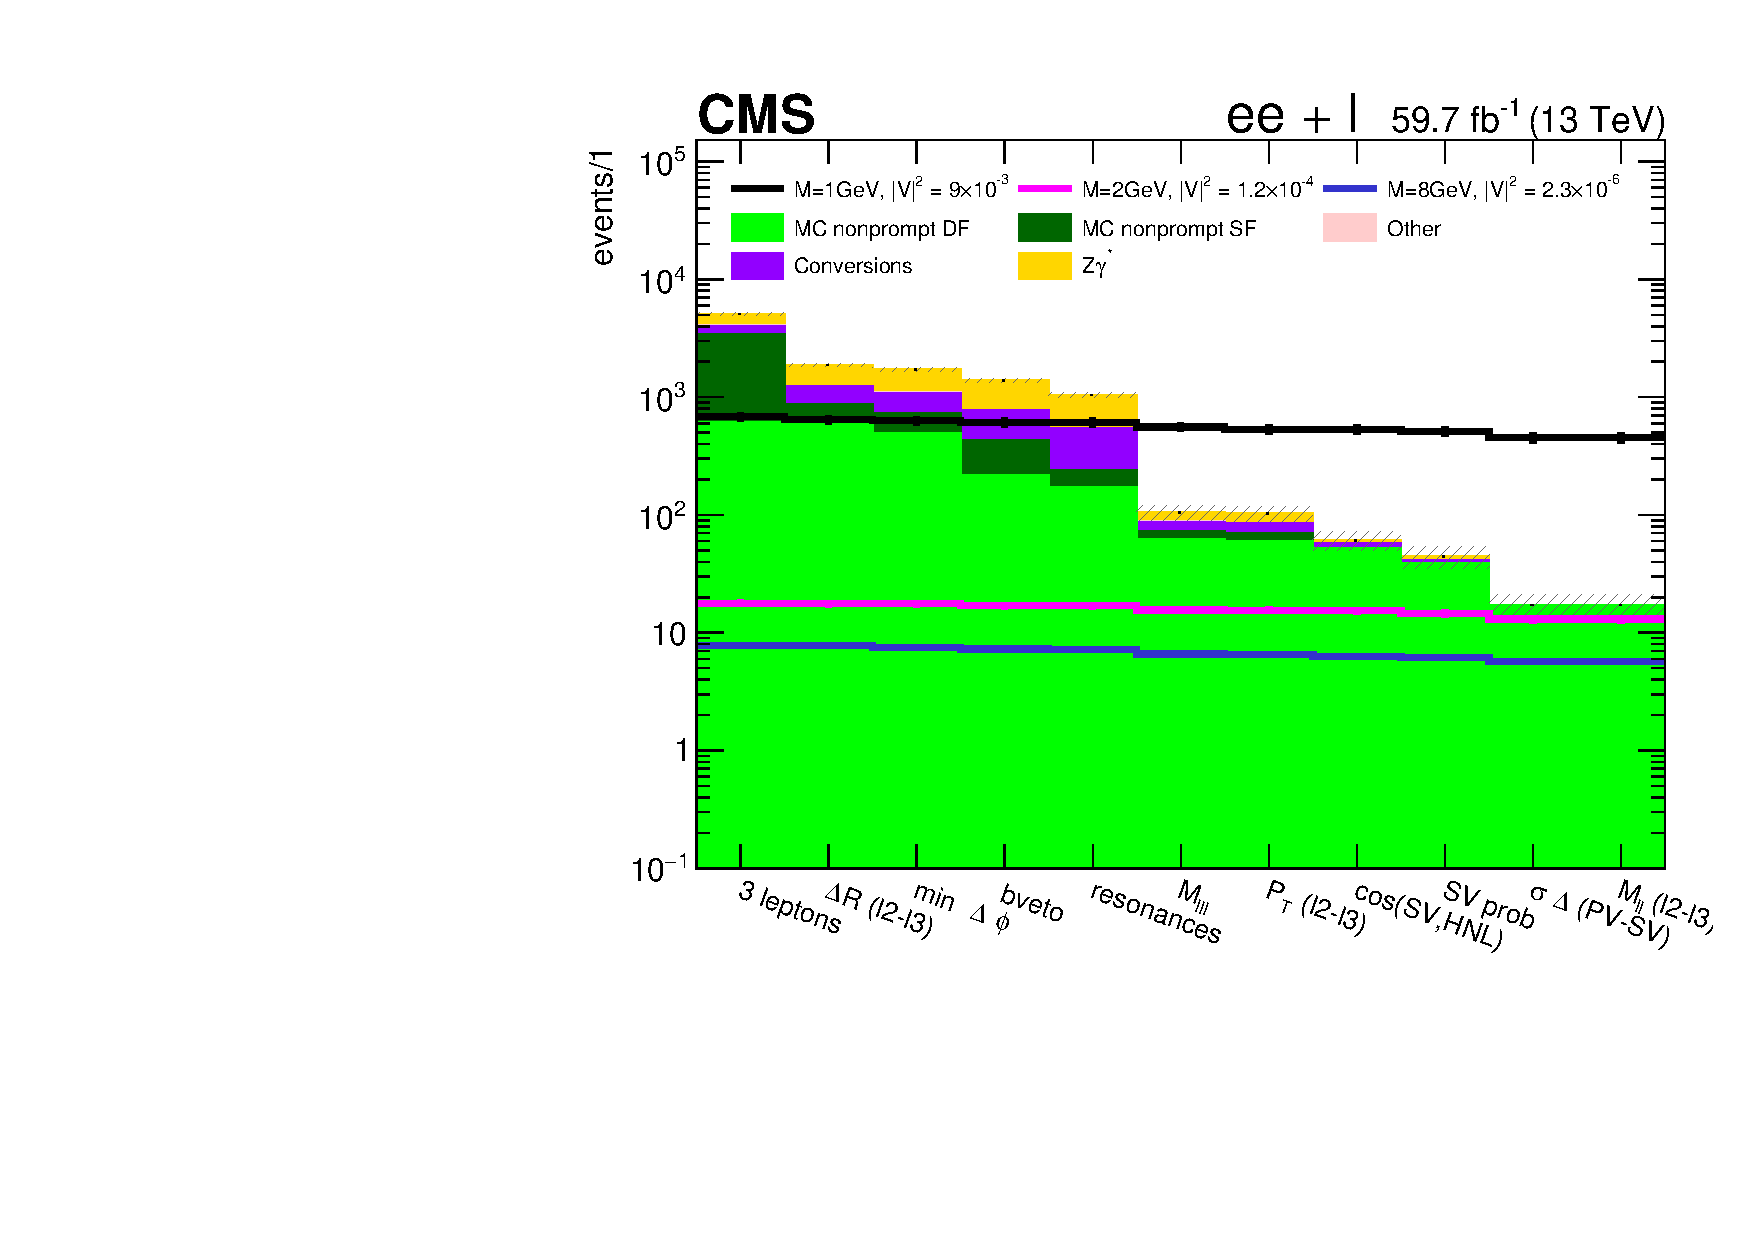
\includegraphics[clip,trim=0.9cm 0.7cm 0.7cm 0.7cm,width=.4\textwidth]{Figures/c6/selection/18/e_cutflow__0.pdf}
  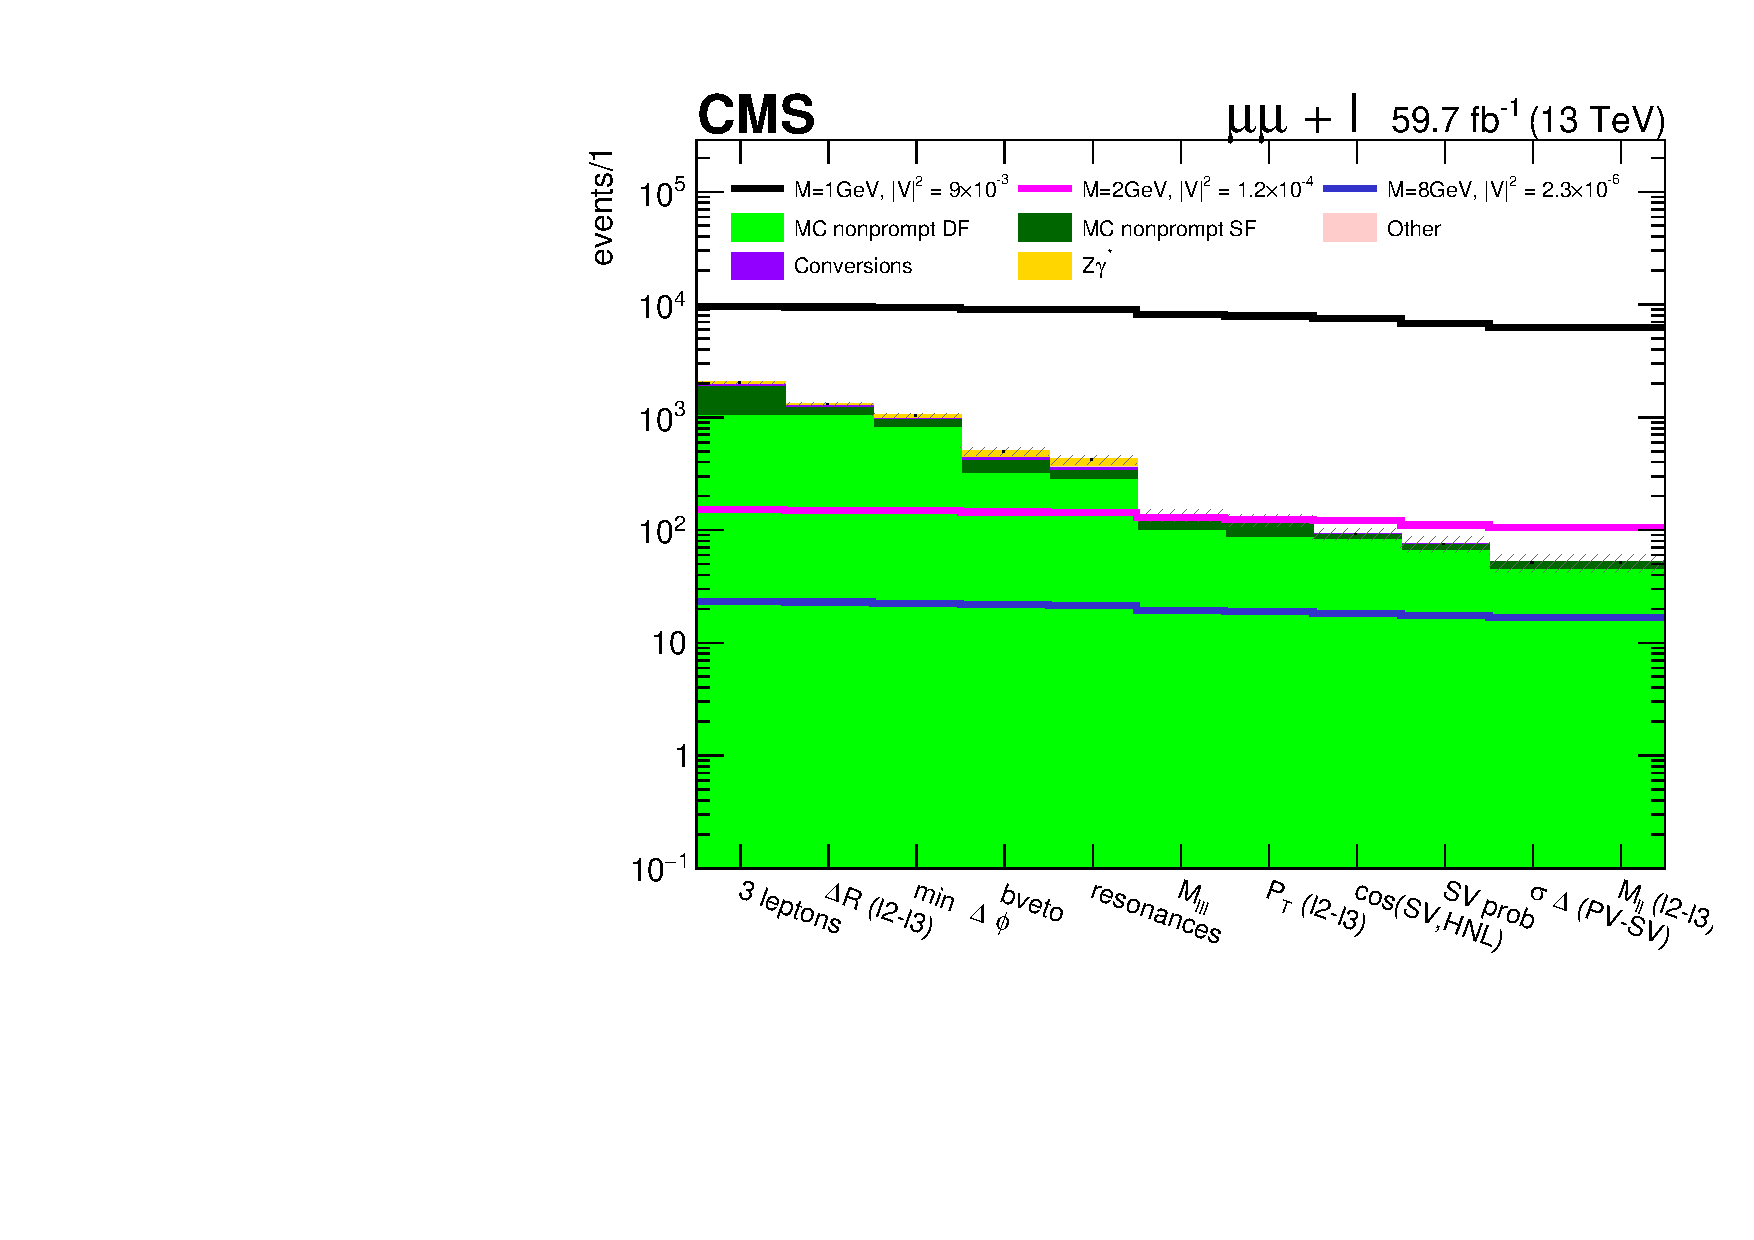
\includegraphics[clip,trim=0.9cm 0.7cm 0.7cm 0.7cm,width=.4\textwidth]{Figures/c6/selection/18/mu_cutflow__0.pdf}\\
  \caption{Cutflow plots showing the full selection applied in simulated backgrounds using the 2018 MC samples,
    in \eex (left) and \mmx (right) final states.
    Signal models for different values of \mhnl and \mixpar
    are shown as empty histograms. For illustration purposes we show
    only the predictions corresponding to 2018 data-taking and luminosity.}
  \label{fig:cutflow1}
\end{figure}

\begin{figure}[h!]
\centering
   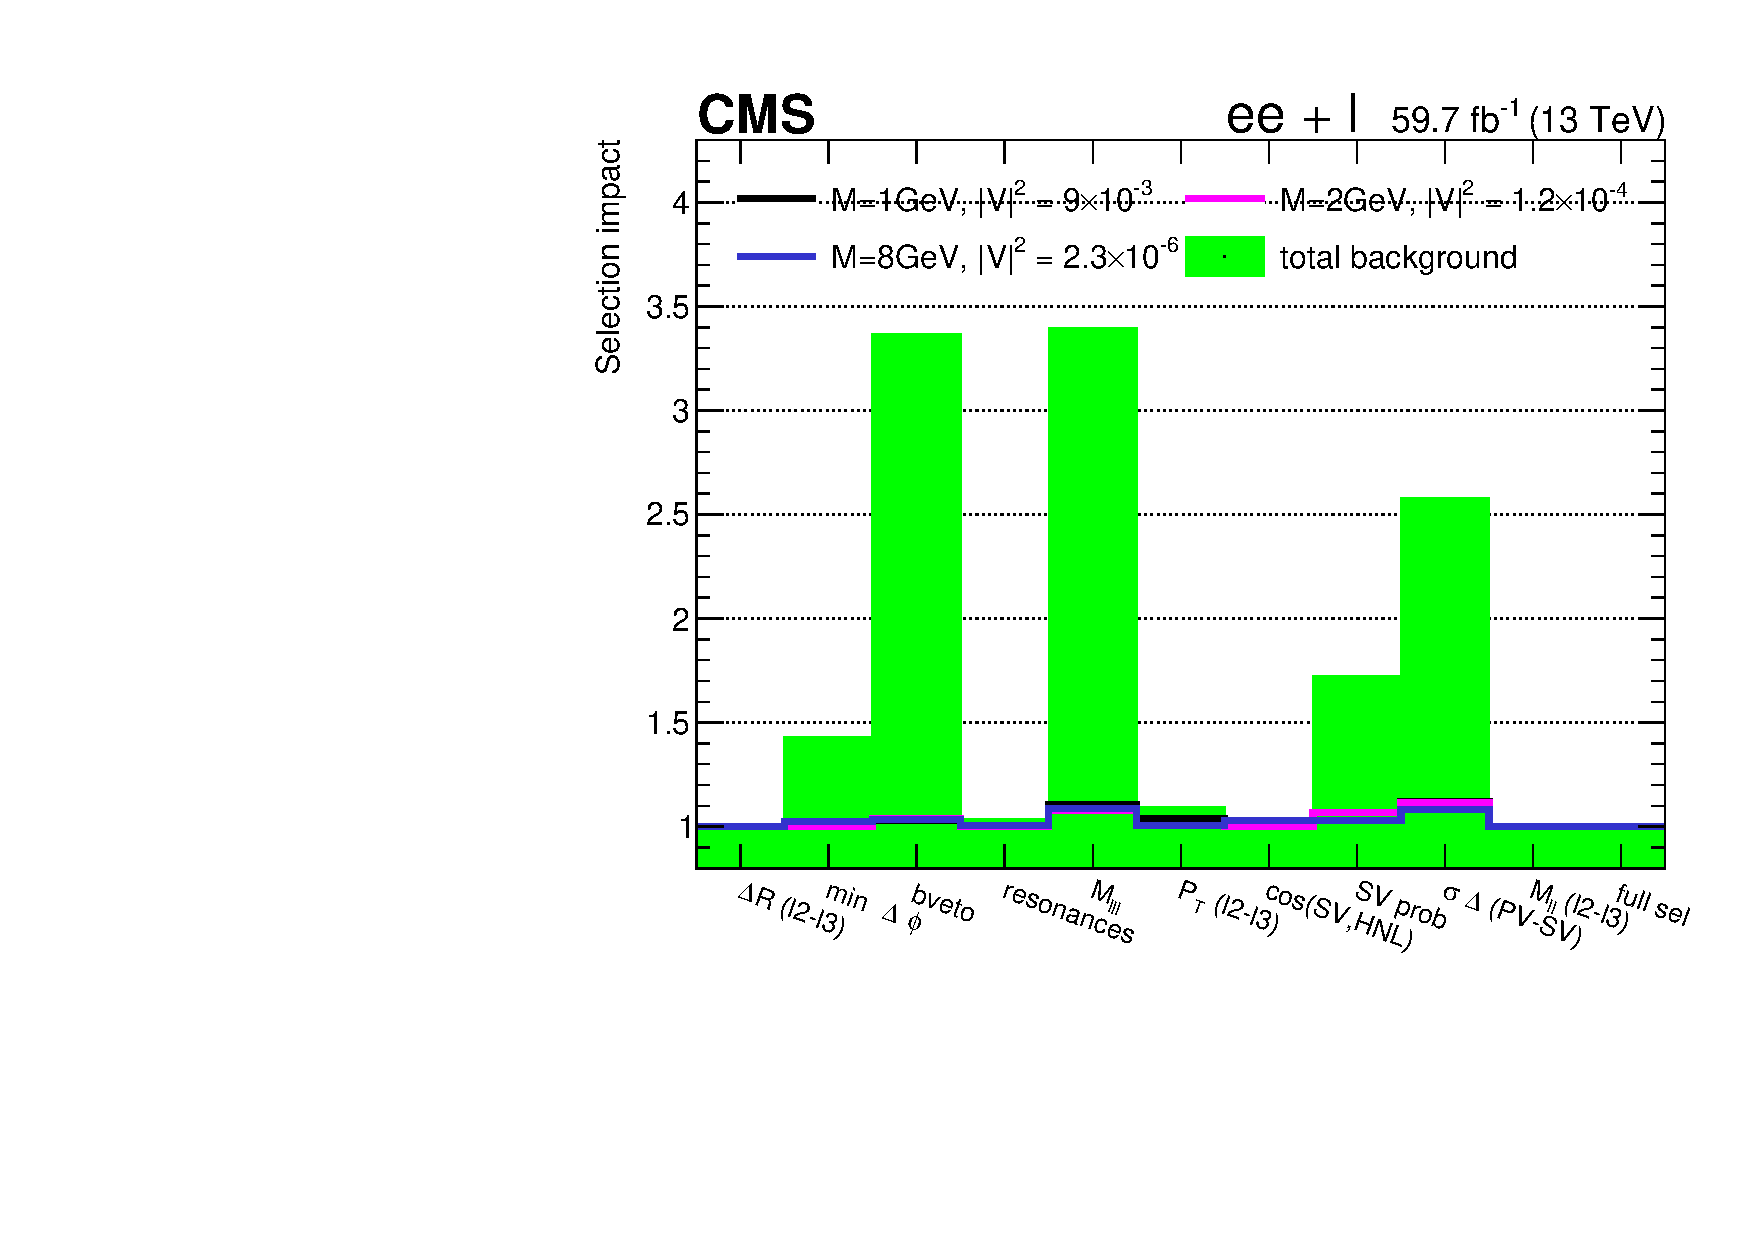
\includegraphics[clip,trim=0.9cm 0.7cm 0.7cm 0.7cm,width=.4\textwidth]{Figures/c6/selection/eff_e_cutflow_n_1__0.pdf}
  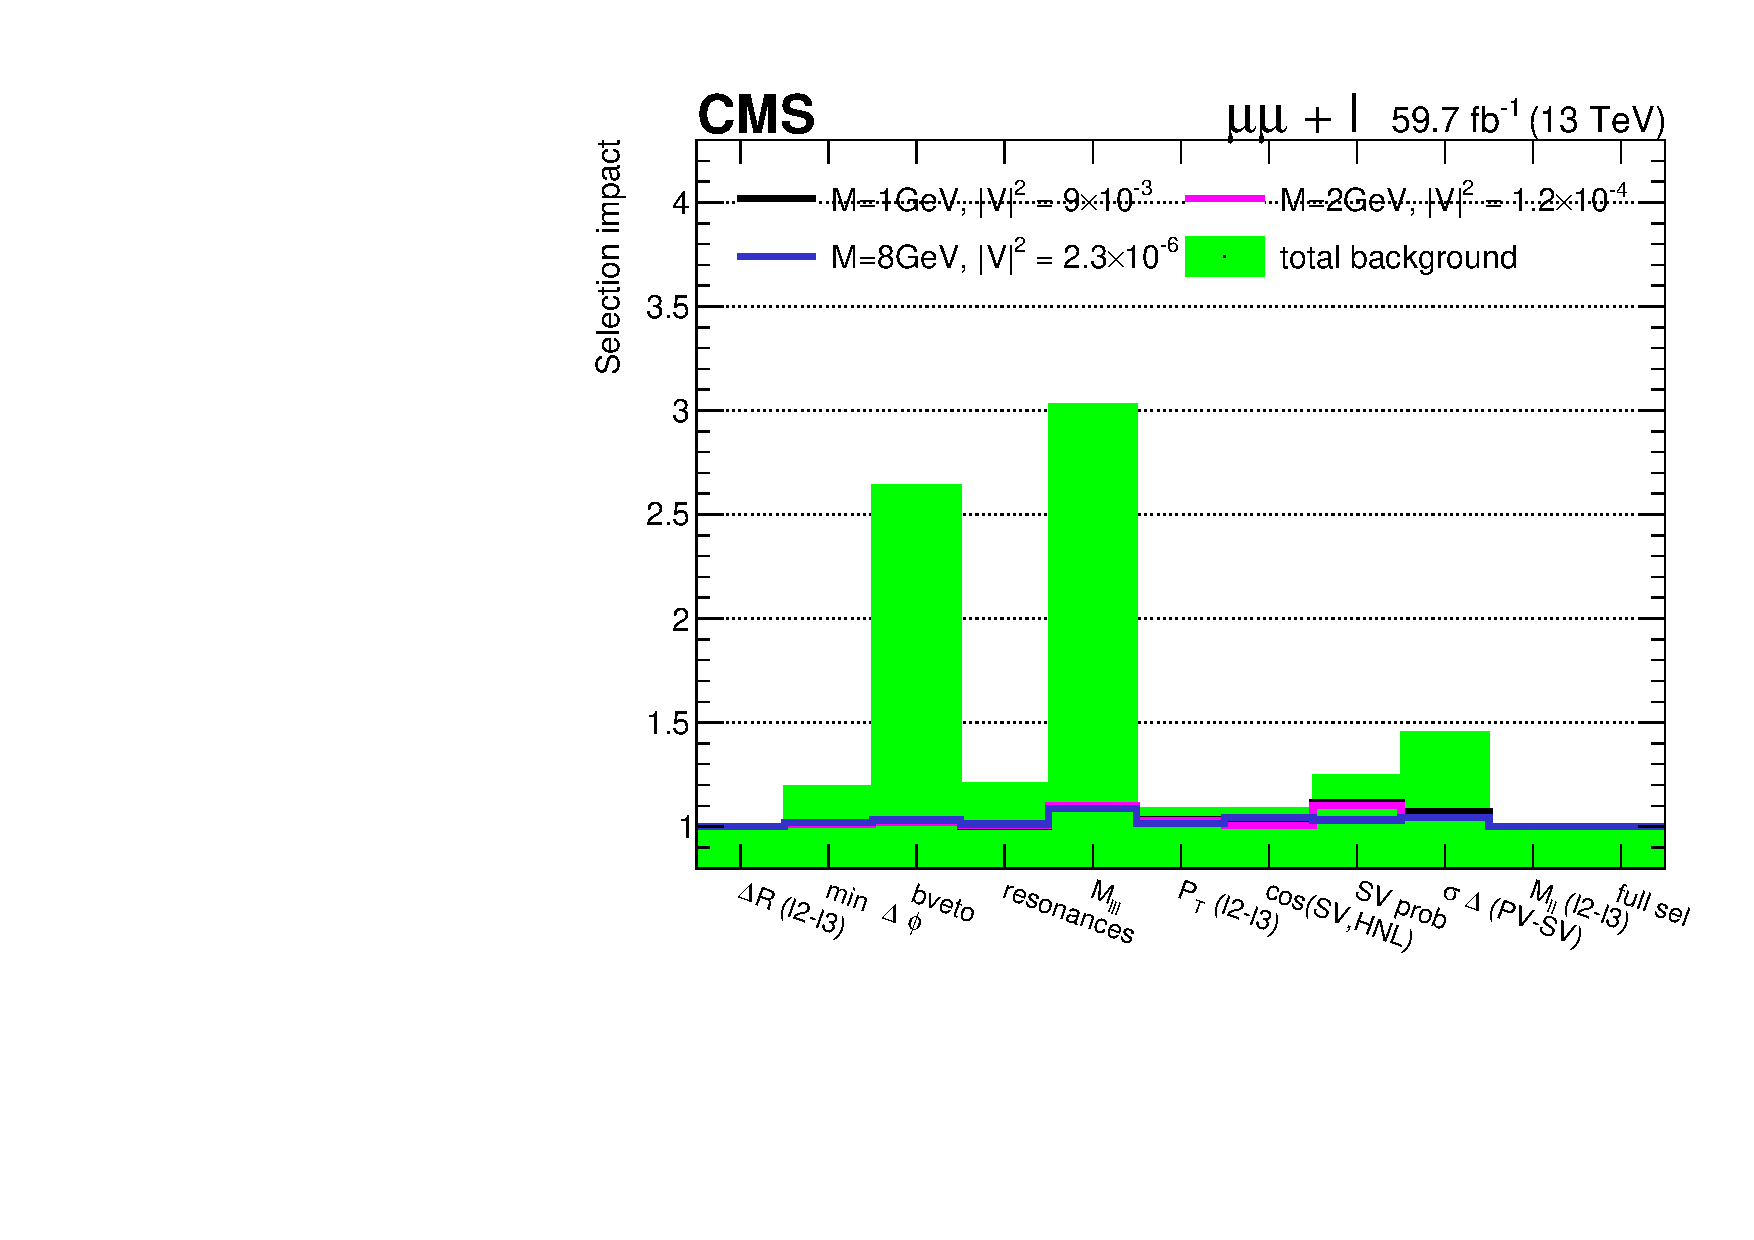
\includegraphics[clip,trim=0.9cm 0.7cm 0.7cm 0.7cm,width=.4\textwidth]{Figures/c6/selection/eff_mu_cutflow_n_1__0.pdf}
  \caption{
   $N-1$ plots but showing the impact in percentage of the single cut (each bin is $yield_{bin}/yield_{full\:selection}$).
    Signal models for different values of \mhnl and \mixpar
    are shown as empty histograms. For illustration purposes we show
    only the predictions corresponding to 2018 data-taking and luminosity.}
  \label{fig:cutflow2}
\end{figure}
\vspace{2mm}


Figure~\ref{fig:reco_displ} shows the transverse
distance of the SV from the PV, \Deltwod, for events
passing the full baseline selection. \Deltwod is the most important
experimental observable to discriminate signal from background.

In the region of large displacement, the sensitivity of the analysis
greatly increases, with a relatively low abundance of nonprompt lepton
background and being virtually free of prompt lepton background
contributions. This represents the key feature of the analysis.
On the contrary, HNL signals with higher masses are short-lived and
they decay in low displacement regions, where both the prompt and
nonprompt lepton contributions are large, similarly to the previous
CMS search presented in Chapter~\ref{Chapter5}.
Although the sensitivity of the analysis strongly depends on the
secondary vertex displacement, no selection is applied on this
variable. This is due to the fact that both small and large
displacement regions are interesting for the search. The small
displacement region represents the region of the previous CMS search
and can be used to cross-check its results, while the large
displacement region provides the highest sensitivity to long-lived
HNLs. 
Thus, the final signal region will be divided into bins of different
displacement, in addition to the invariant mass of \ltwo and \lthree,
\mtwol (Figure~\ref{fig:reco_displ}).\\

The residual background, dominated by \Xg,
$\PZ/\PGg^{\ast}+\mathrm{jets}$, and top processes, accumulates at low
displacement. The HNL signal models populate higher \Deltwod bins, depending on \mhnl and \mixpar. In particular, \Deltwod
is found to provide the best discrimination between signal and
background, and among different signal models.
Therefore we select four event categories, based on the value of
\Deltwod, with different sensitivities for different signal
scenarios:
$\Deltwod<0.5$\cm (fully background dominated), $0.5<\Deltwod<1.5$\cm,
$1.5<\Deltwod<4$\cm and $\Deltwod>4$\cm.\\
In addition, the events are split into three different categories
according to lepton flavors. In case 
the muon coupling is been probed the 3 final states are $\mu\mu\mu$,  $\mu^{\mp}\mu^{\pm} e$ 
and $\mu^{\pm}\mu^{\pm}e$; in case of electron coupling the 3 final states
are: $eee$,  $e^{\mp}e^{\pm}\mu$ and $e^{\pm}e^{\pm}\mu$. This latter categorization
is necessary to provide separated limits for the case of LNC 
and for the case LNV, (see Section~\ref{sec:lnv_lnc}).
The different categories are also characterized by different
background levels and composition, thus providing different
sensitivities.

Finally, we notice that the top background processes, where \ltwo and
\lthree are typically produced in the semi-leptonic decay of $B$
hadrons, populate a region of $\mtwol<4$\GeV, and are basically absent
at higher dilepton masses. Therefore we further split the data into
two categories: $\mtwol<4$\GeV and $\mtwol>4$\GeV.\\
 
 \begin{wrapfigure}{r}{0.62\textwidth}
  \centering
  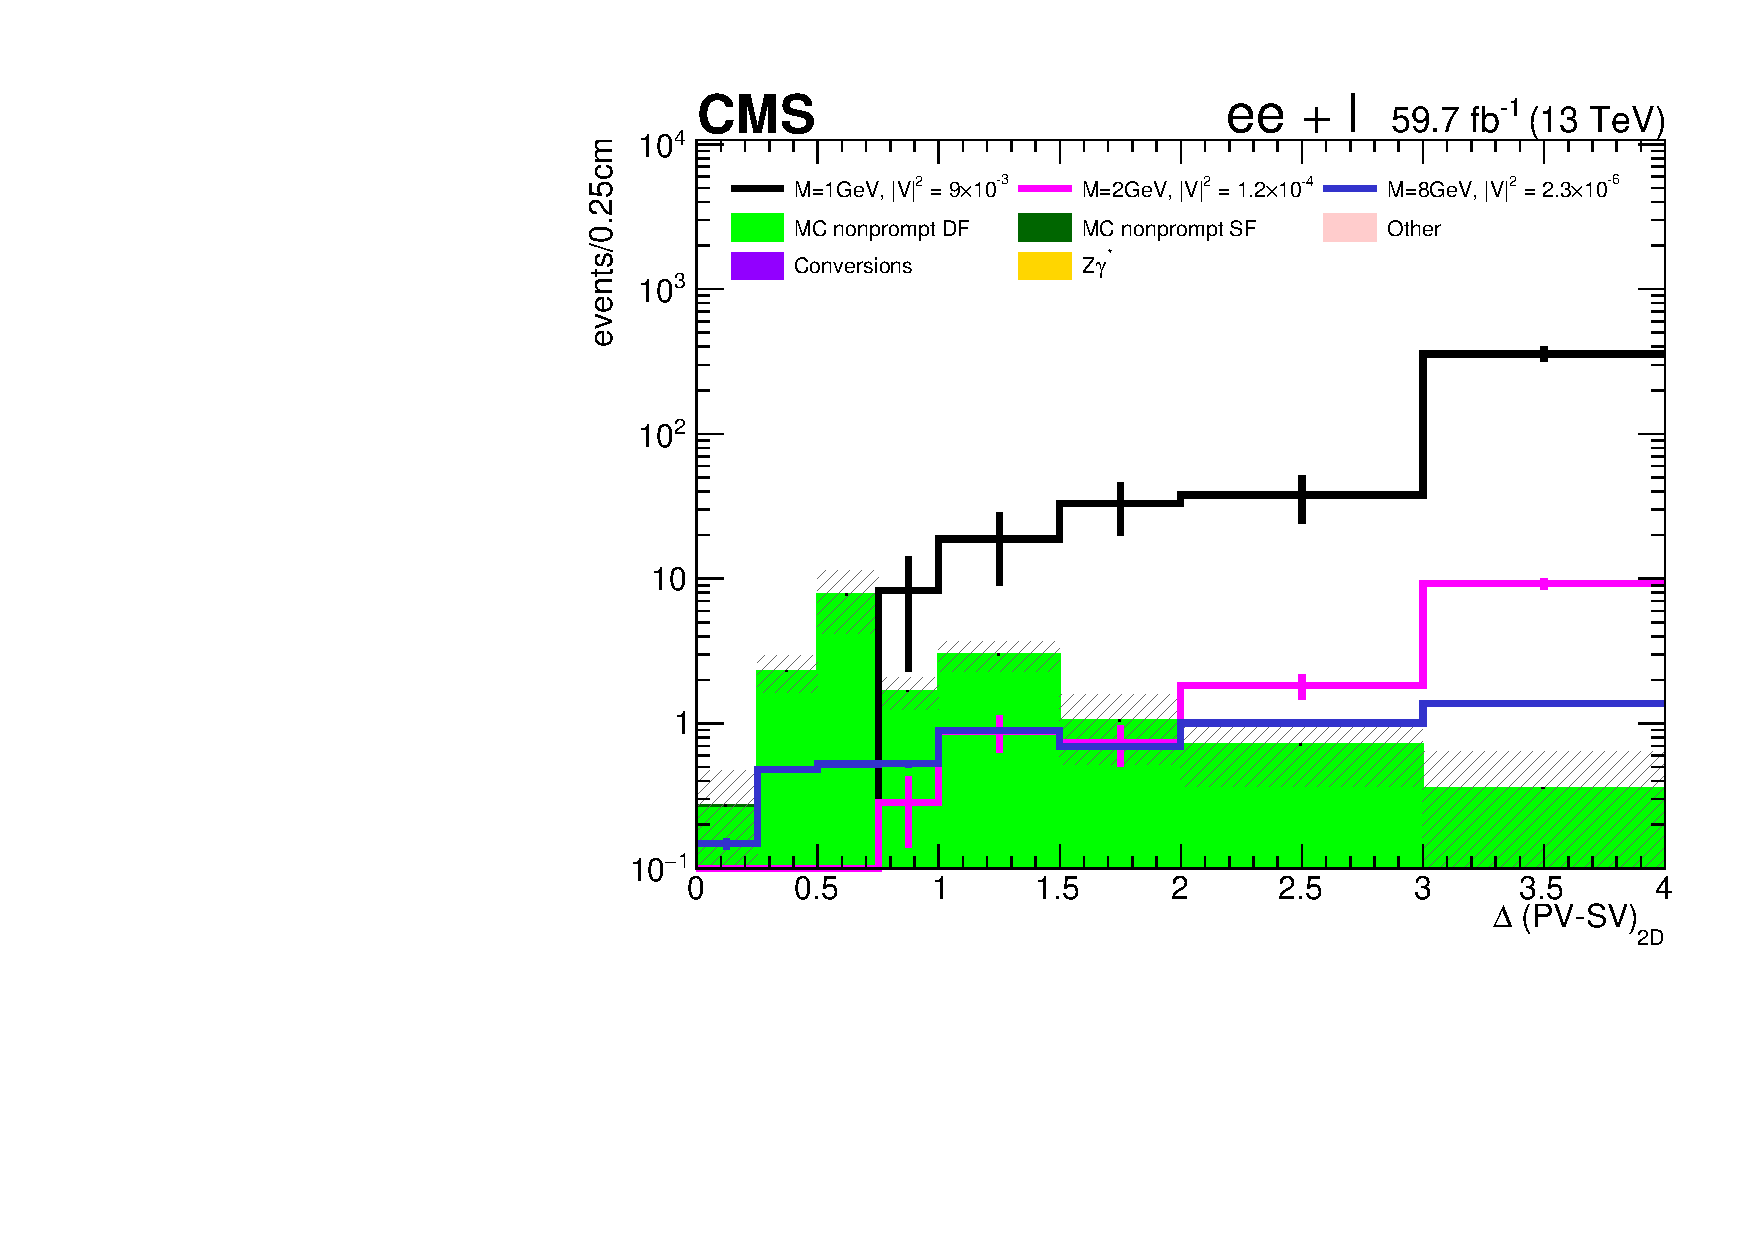
\includegraphics[clip,trim=0.9cm 0.7cm 0.7cm 0.9cm,width=.3\textwidth]{Figures/c6/selection/18/e_DeltaPV_SV_2D_zomm__final.pdf}
  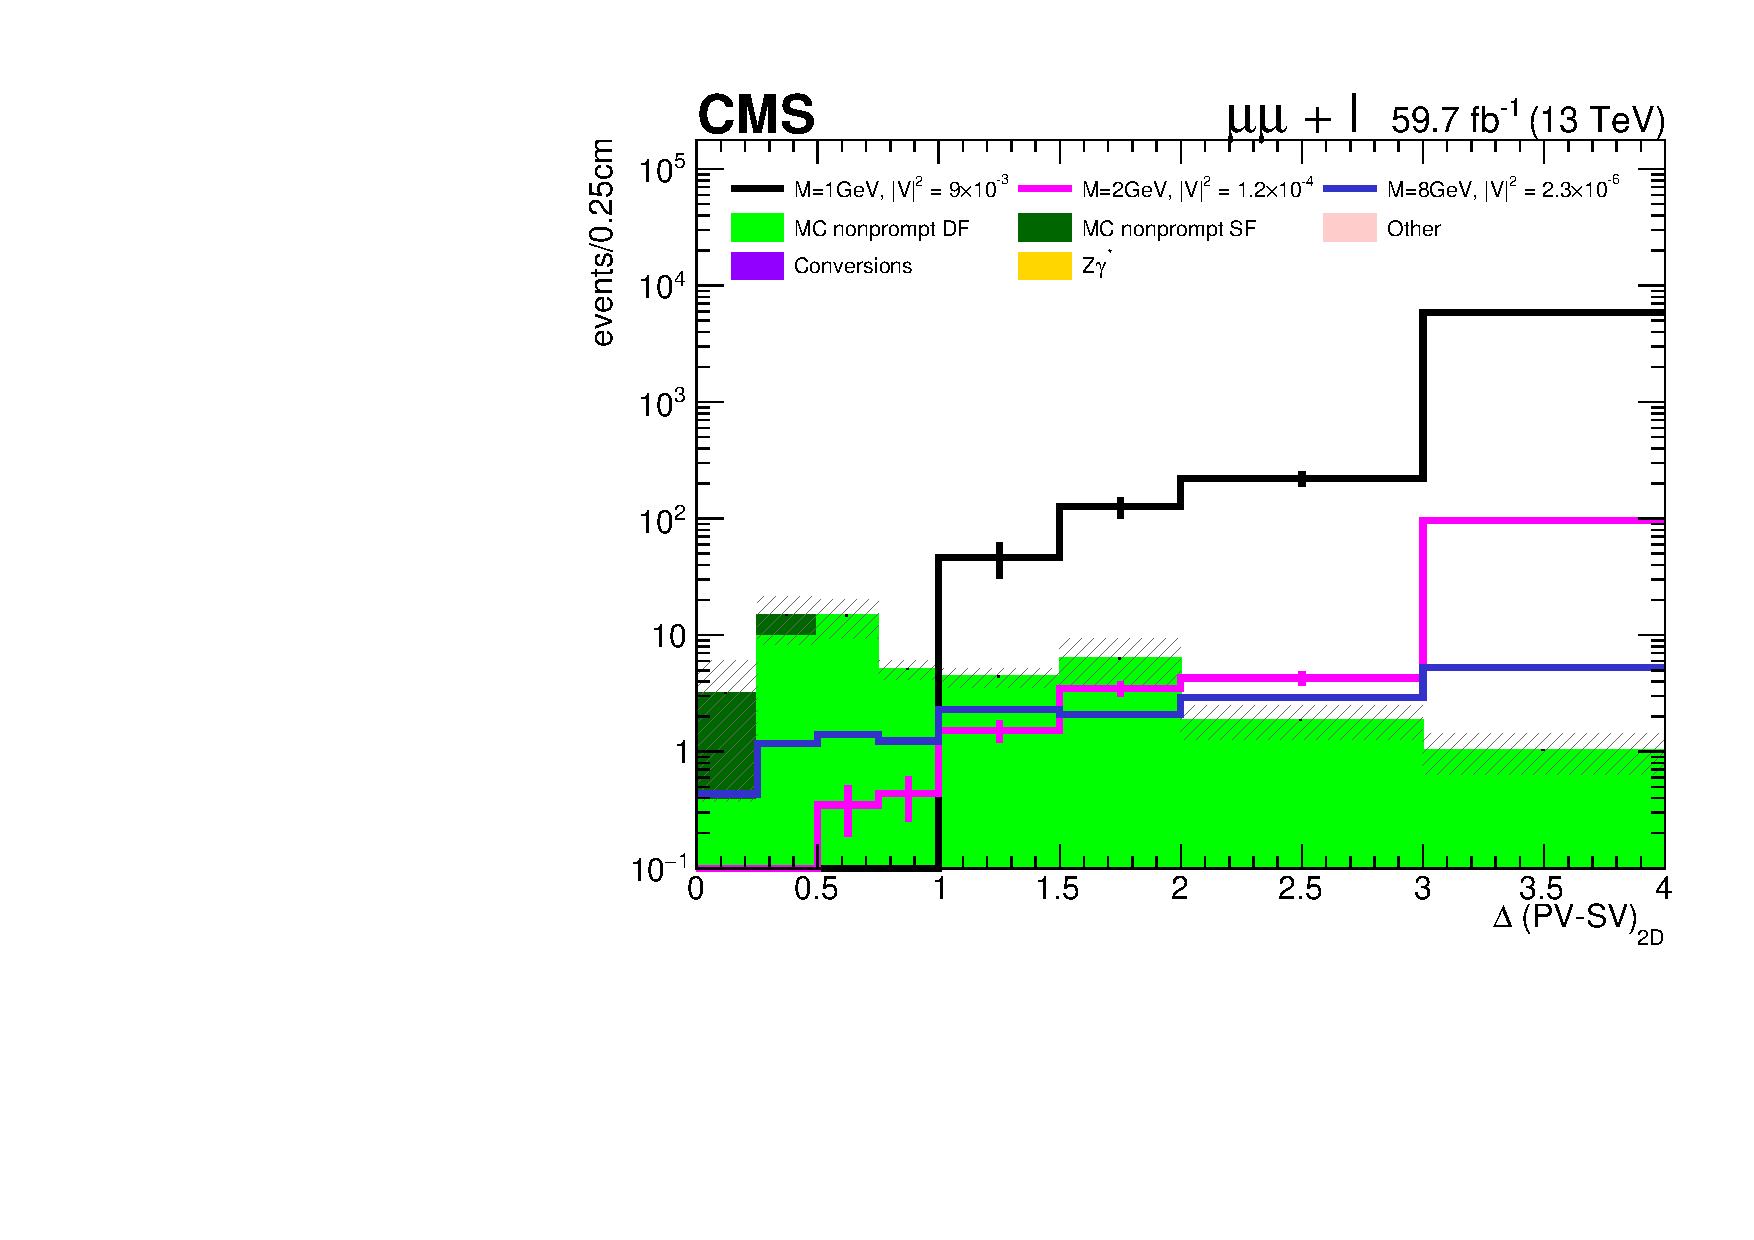
\includegraphics[clip,trim=0.9cm 0.7cm 0.7cm 0.9cm,width=.3\textwidth]{Figures/c6/selection/18/mu_DeltaPV_SV_2D_zomm__final.pdf}\\
  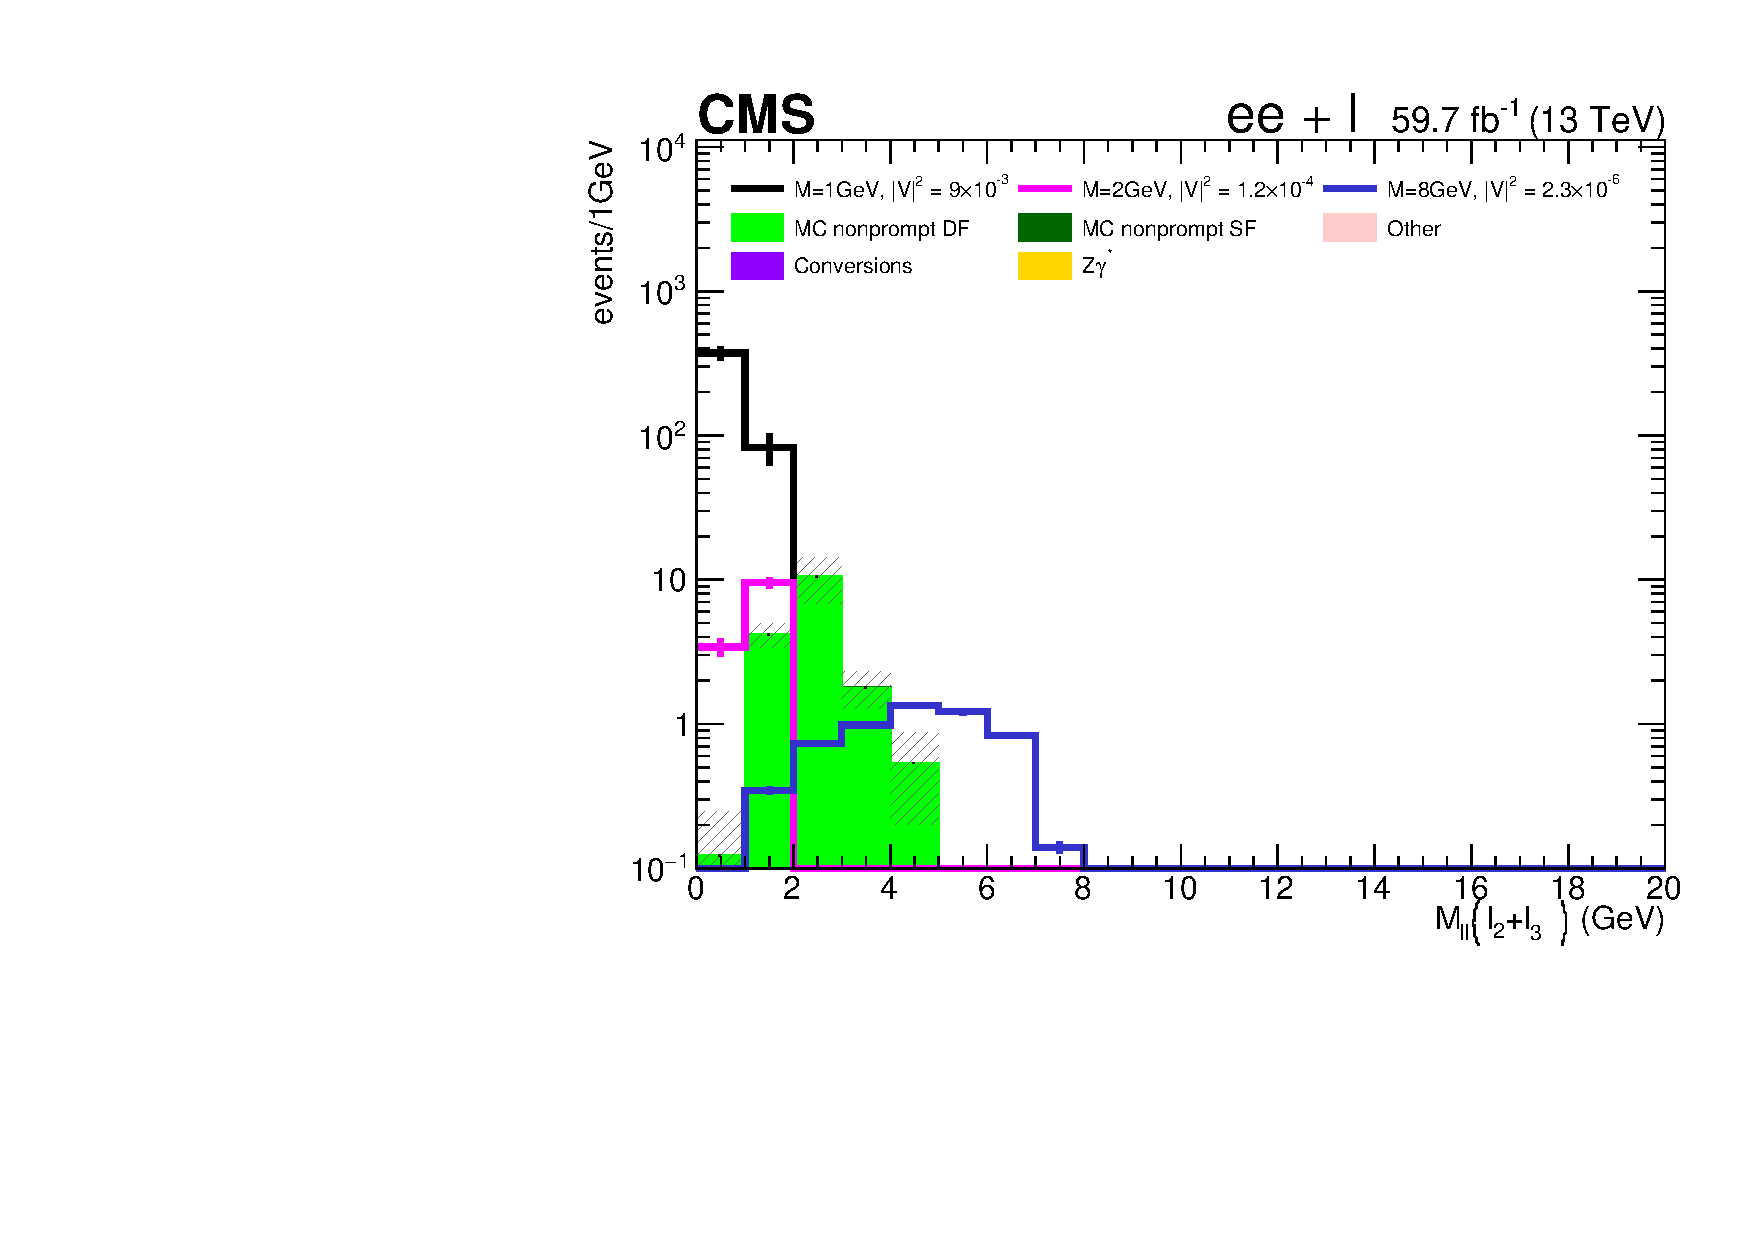
\includegraphics[clip,trim=0.9cm 0.7cm 0.7cm 0.9cm,width=.3\textwidth]{Figures/c6/selection/18/e_M_ll_l2_l3_zoom__final.pdf}
  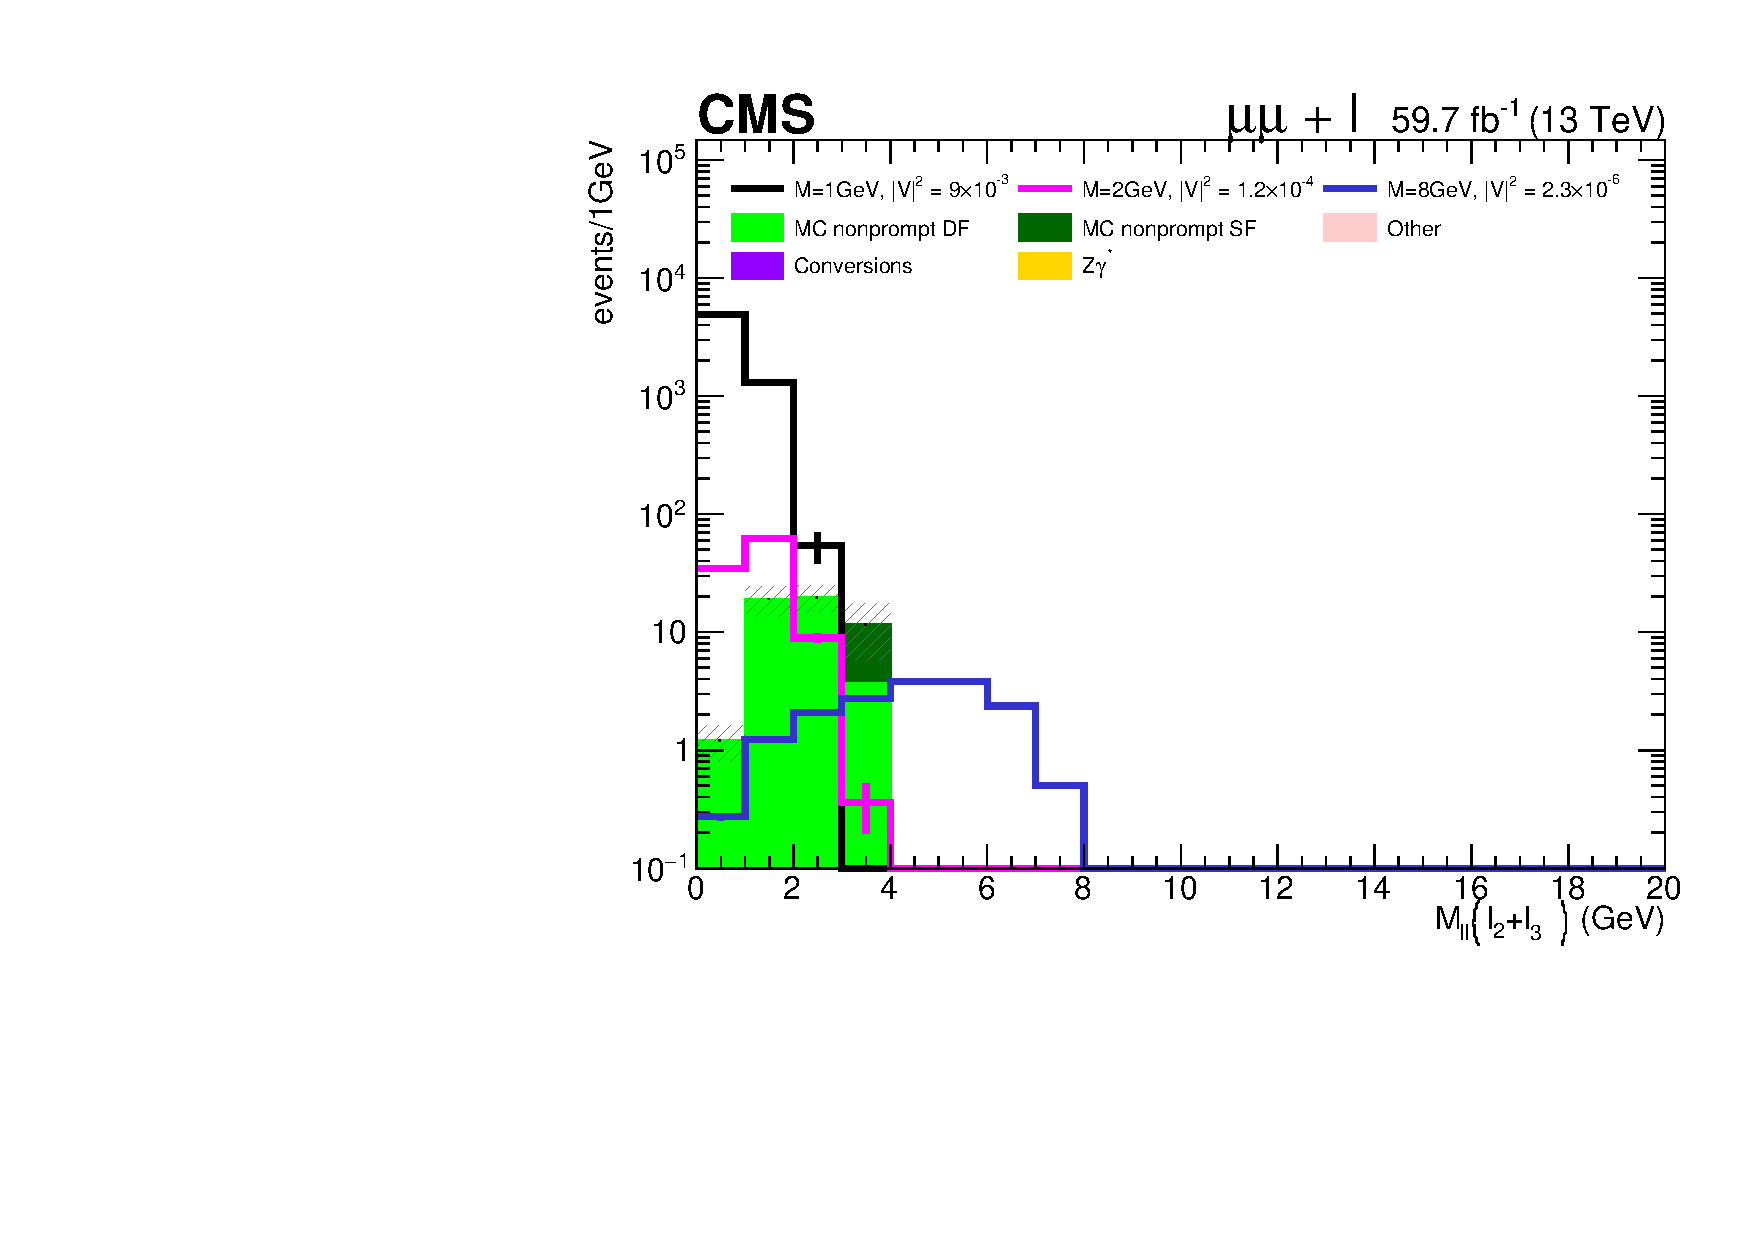
\includegraphics[clip,trim=0.9cm 0.7cm 0.7cm 0.9cm,width=.3\textwidth]{Figures/c6/selection/18/mu_M_ll_l2_l3_zoom__final.pdf}
  \caption{\Deltwod (left), and $M_{\ltwo \lthree}$ (right) in events
    passing the baseline selection of Table~\ref{tab:baselinesel}. For illustration purposes we show
    only the predictions corresponding to 2018 data-taking and luminosity.}
  \label{fig:reco_displ}
\end{wrapfigure}

Due to the lack of statistic (in background) at large displacement
bins for high mass region, it has
 been decided to reduce the number of bins 
in the following way:
\begin{itemize}
\setlength\itemsep{-0.5em}
\item for $\mtwol<4$\GeV
  \begin{itemize}
    \setlength\itemsep{-0.3em}
    \item $\Deltwod<0.5$\cm
    \item $0.5<\Deltwod<1.5$\cm
    \item $1.5<\Deltwod<4$\cm
    \item $\Deltwod>4$\cm
  \end{itemize}  
\item for $\mtwol>4$\GeV
\begin{itemize}
    \setlength\itemsep{-0.3em}
    \item $\Deltwod<0.5$\cm
    \item $\Deltwod>0.5$\cm
  \end{itemize}  
\end{itemize}



\comm{
All the distributions previously shown contain background predictions using only MC samples and 
do not have any data points.
At this stage of the analysis process we do not want to show any data-yield since it is not clear yet if 
the background estimation using only MC can predict well the behavior of the data. To ensure so, 
we should first check in regions orthogonal with respect to signal region if the MC can predict the data; if it is not the case 
it is important to find a way to predict the contribution of the background using directly data: data-driven estimation.

All the distributions previously shown contain background predictions using only the 2018 MC samples; 2016 and 2017 can be found in Appendix~\ref{app:appendix_MC_2017_2018}.}
\clearpage
%%%%%%%%%%%%%%%%%%%%%%%%%%%%%%%%%%%%%%%%%%%%%%%%%%%%
%%%%%%%%%%%%%%%%%%%%%%%%%%%%%%%%%%%%%%%%%%%%%%%%%%%%
%%%%%%%%%%%%%%%%%%%%%%%%%%%%%%%%%%%%%%%%%%%%%%%%%%%%
\section{Background estimation}\label{sec:llbackground}
\subsection{Background composition}\label{sec:llcomposition}

The main SM background processes mimicking the signal final states can be
classified as follows.
\begin{itemize}
\item \textbf{``Fake'' nonprompt leptons (\Pe or \PGm):}
  muons from light-flavor mesons that decay in flight, or electrons from
  unidentified conversions of photons in jets
  can mimic the \displ leptons from the HNL decay, \ltwo and
  \lthree.
  This background is dominated by top--quark and Drell--Yan processes,
  and is measured with the data-driven method described in
  Section~\ref{sec_llfakelepton}.\\
In most of the analyses --like the one presented in Chapter~\ref{Chapter5}-- this
background consists of events where one lepton is fake. 
In this search, the particular event selection leads to the two
displaced leptons being fake as the majority of this background and thus, it needs to be handled properly.
Therefore fake nonprompt lepton
backgrounds are split into two categories:
  \begin{itemize}
  \item \textbf{single fake nonprompt leptons}:
    a single reconstructed lepton produced via one of the above
    mechanisms, \eg the (semi-)leptonic decay of a meson.
    Multiple single-fake leptons can be found in an event,
    produced in the independent decays of different mesons.
    In this case, the probabilities to select different fake nonprompt
    leptons for the analysis can be treated as uncorrelated.
  \item \textbf{double fake nonprompt leptons}:
    a pair of reconstructed leptons produced in the decay chain of the
    same hadron, typically a $B$ meson (\eg via
    $b\to\ell^-\bar{\PGn}_{\ell}\PQc\to\ell^-\bar{\PGn}_{\ell}\ell^{\prime+}\PGn_{\ell^{\prime}}\PQs$)
    or a quarkonium state (\eg $\JPsi\to\ell^-\ell^+$).
    In such decays the two leptons are manifestly not independent and
    their selection probabilities are strongly correlated.
    Therefore, the lepton pair must be treated as a single system.
  \end{itemize}
\item \textbf{Photon conversions:} this background was extensively
  introduced in Sections~\ref{sec:c4photon} and~\ref{sec:bgk}.\\
  It is estimated from simulation and verified in control regions with
  three leptons forming a \PZ mass (Section~\ref{sec:conversion}).
  Such conversions are considered as a
  source of a background, as well as an excellent probe for nonprompt
  lepton efficiency
 measurement, in many searches for displaced vertices.

\end{itemize}
 
\subsection{Fake-lepton background}\label{sec_llfakelepton}
The fake-lepton background is estimated using the \ttol
method.
A general description of the fake-rate method can be found in
Section~\ref{sec:tight_loose_method}.\\
For this search, the probability for 
a fake lepton to pass the \tD (Tables~\ref{tab:electronSelection} and \ref{tab:muonSelection}) and isolation requirements is estimated by using event yields where at least one lepton fails to satisfy \tD 
selection criteria but passes
\fo ones~\footnote{We all agree that \ttol naming is not optimal when the
  ratio happens between \tD and \fo leptons. For ``historical'' and ``traditional''
  reasons we use \ttol name keeping in mind that the selection in the
  denominator is the \fo one.}.

The main difference with respect to the prompt HNL analysis
(Chapter~\ref{Chapter5}) comes from the different sources of fake
leptons; here fake leptons are typically found in the proximity of a
jet which is in common for both \ltwo and \lthree, and their
experimental properties are correlated. Each \fo
lepton is therefore associated to the jet of $\pt>10$\GeV closest in
\DR, \ie $\DR<0.4$.
If two \fo leptons 
are either associated to the same jet or have $\DR<0.45$, they are considered double-fake
leptons and treated as a single dilepton system.
In all other cases --- \ie, if the two \fo leptons are associated to
different jets and the $\DR>0.45$ ---,
the \fo leptons are considered single fakes and (if more than one)
treated independently.

An important clarification has to be made regarding the estimation of 
the fake-lepton background. This prediction only accounts for 
fake ``displaced''  (\ltwothree) leptons. The contribution from
fake prompt (\ie \lone) leptons is expected to be very small, on
account of the much higher probability for fake \ltwo and \lthree to
pass the tight \displ selection. This assumption has been verified in
MC using the information at generated level (MC truth); at the
beginning of the selection only 1\textperthousand\ background
events have fake nonprompt \lone, at the end of the selection all \lone
leptons are prompt leptons, which ensures that the contribution from
pure QCD processes is negligible. 
For this reason, the contribution from fake \lone is neglected.

\subsubsection{Estimation of double-fake background}
\label{sec:doubleFakeBkg}

Events in the application region are classified as double-fake
background if the two fake leptons are either associated to the same
jet or the distance between them is $\DR<0.45$, and at least one of them is \fo.
In the first case (same jet associated), the \pt of the mother parton, \ptm from
which the fake leptons originate is estimated using the \pt of the associated
jet, $\ptm=\ptj$, calibrated using jet energy corrections (JEC, see
Section~\ref{sec:jetclustering}) after subtracting the \pt of the two leptons:
\begin{linenomath}
  \begin{equation}
    \label{eq:ptjet}
    \ptm = \ptj =
    \left(\pt^{\mathrm{raw\,jet}}-\pt^{\ltwo}-\pt^{\lthree}\right)\times\mathrm{JEC}
    \;+\; \pt^{\ltwo} \;+\; \pt^{\lthree}.
  \end{equation}
\end{linenomath}
In this formula, all the \pt are 4-vectors.
Similar is the case when the distance between them is $\DR<0.45$:
\begin{linenomath}
  \begin{equation}
    \label{eq:ptjet_45}
    \ptm = \ptj = p^{jet,2}_T + p^{jet,3}_T 
  \end{equation}
\end{linenomath}
where the $p^{jet,i}$ is the jet associated to the lepton \emph{i} and then corrected using the JEC right correction:
\begin{linenomath}
  \begin{equation}
    \label{eq:ptjet_45_single}
    p_T^{jet,i} = \left(\pt^{\mathrm{raw\,jet_i}}-\pt^{\ell_{i}}\right)\times\mathrm{JEC}\;+\; \pt^{\ell_i} .
  \end{equation}
\end{linenomath}

\Dfr (\dfr) is parametrized and applied as a
function of the \pt of the associated jet:
$\dfr=\dfr(\ptj)$.
The definition of the measurement region is similar to that of the
signal region, with the following differences:
\begin{itemize}
\setlength\itemsep{-0.2em}
\item the two fake leptons, \ltwo and \lthree, are selected with
  the \fo identification criteria (see
  Tables~\ref{tab:electronSelection} and \ref{tab:muonSelection})
  and must be either associated to the same jet or have $\DR<0.45$;
\item a b-tagged jet with $\pt>25$\GeV must be present (not
  necessarily the same that \ltwo and \lthree are associated to).
\end{itemize}
The requirement of a \PQb enriches the sample in top-quark
backgrounds, which are the main source of double-fake leptons, see Table~\ref{tab:measurement_sel}.
Events in this measurement region have two \fo leptons, of
which zero, one, or both can be \tD.
\begin{table}[h!]
  \centering
{\footnotesize

  \caption{\label{tab:measurement_sel} Measurement region selection requirements
    for double fake.}
    \begin{tabular}{l|l}
    \hline
    Variable     & Requirement       \\
    \hline
    \hline
    N. \PQb & $\geq 1$              \\
    \mtwol in $\Pe\Pe\Pe$& $> 0.5$\GeV              \\ 
    resonance vetoes & \checkmark      \\
    \hline
   %% \mthreel  and  N. \PQb  & ($<50$\GeV or $>80$\GeV N.\PQb = 0) OR  (N.\PQb $\neq$ 0)\\
     \hline
     \mthreel in $\Pe\Pe\Pe$ and $\PGm\PGm\Pe$ OS & $<80$\GeV or $>101$\GeV \\
      \mtwol in $\Pe\Pe\Pe$& $> 0.5$\GeV              \\ 
    \hline
    \hline 
  \end{tabular}
}
\end{table}

The \Dfr, \dfr is defined as the fraction of events in this
region where both \fo leptons pass \tD selection.
Figure~\ref{fig:dFR_ptjet_16} (top) shows
the measured values of \dfr for events with two electrons, an electron
and a muon, and two muons, respectively, as a function of \ptj.
Figure~\ref{fig:dFR_ptjet_16} (bottom) shows
the measured values of \dfr for events with two electrons, an electron
and a muon, and two muons, respectively, as a function of \Deltwod. The \Deltwod bins are the four bins chosen for the SR in order to evaluate 
which is the dependance of the \dfr with respect to the displacement of the SV of the \hnl decay. 

\begin{figure}[h]
  \noindent
\makebox[\textwidth]{
  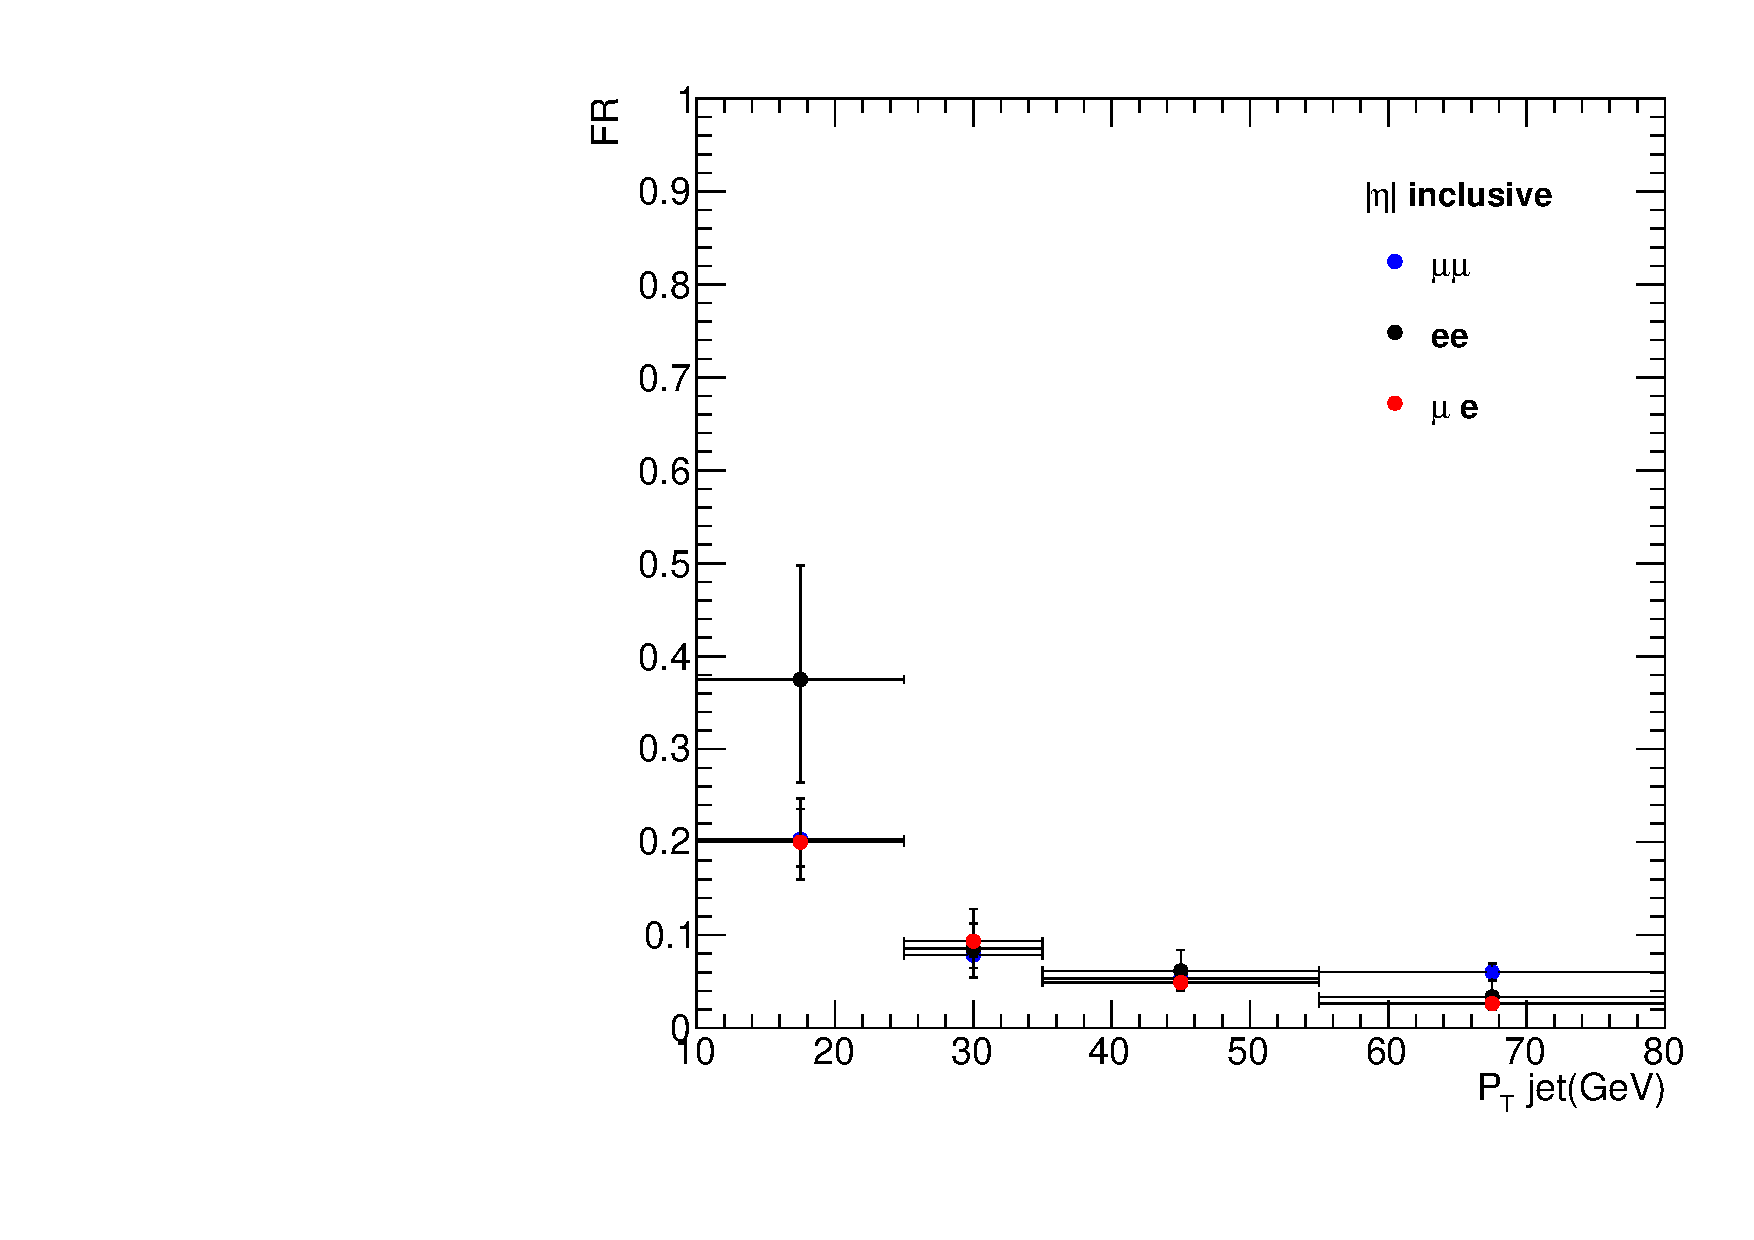
\includegraphics[width=.33\textwidth]{Figures/c6/backgrounds/FR/dFR/16/c_LeptonPt___eta_FR1.pdf}
  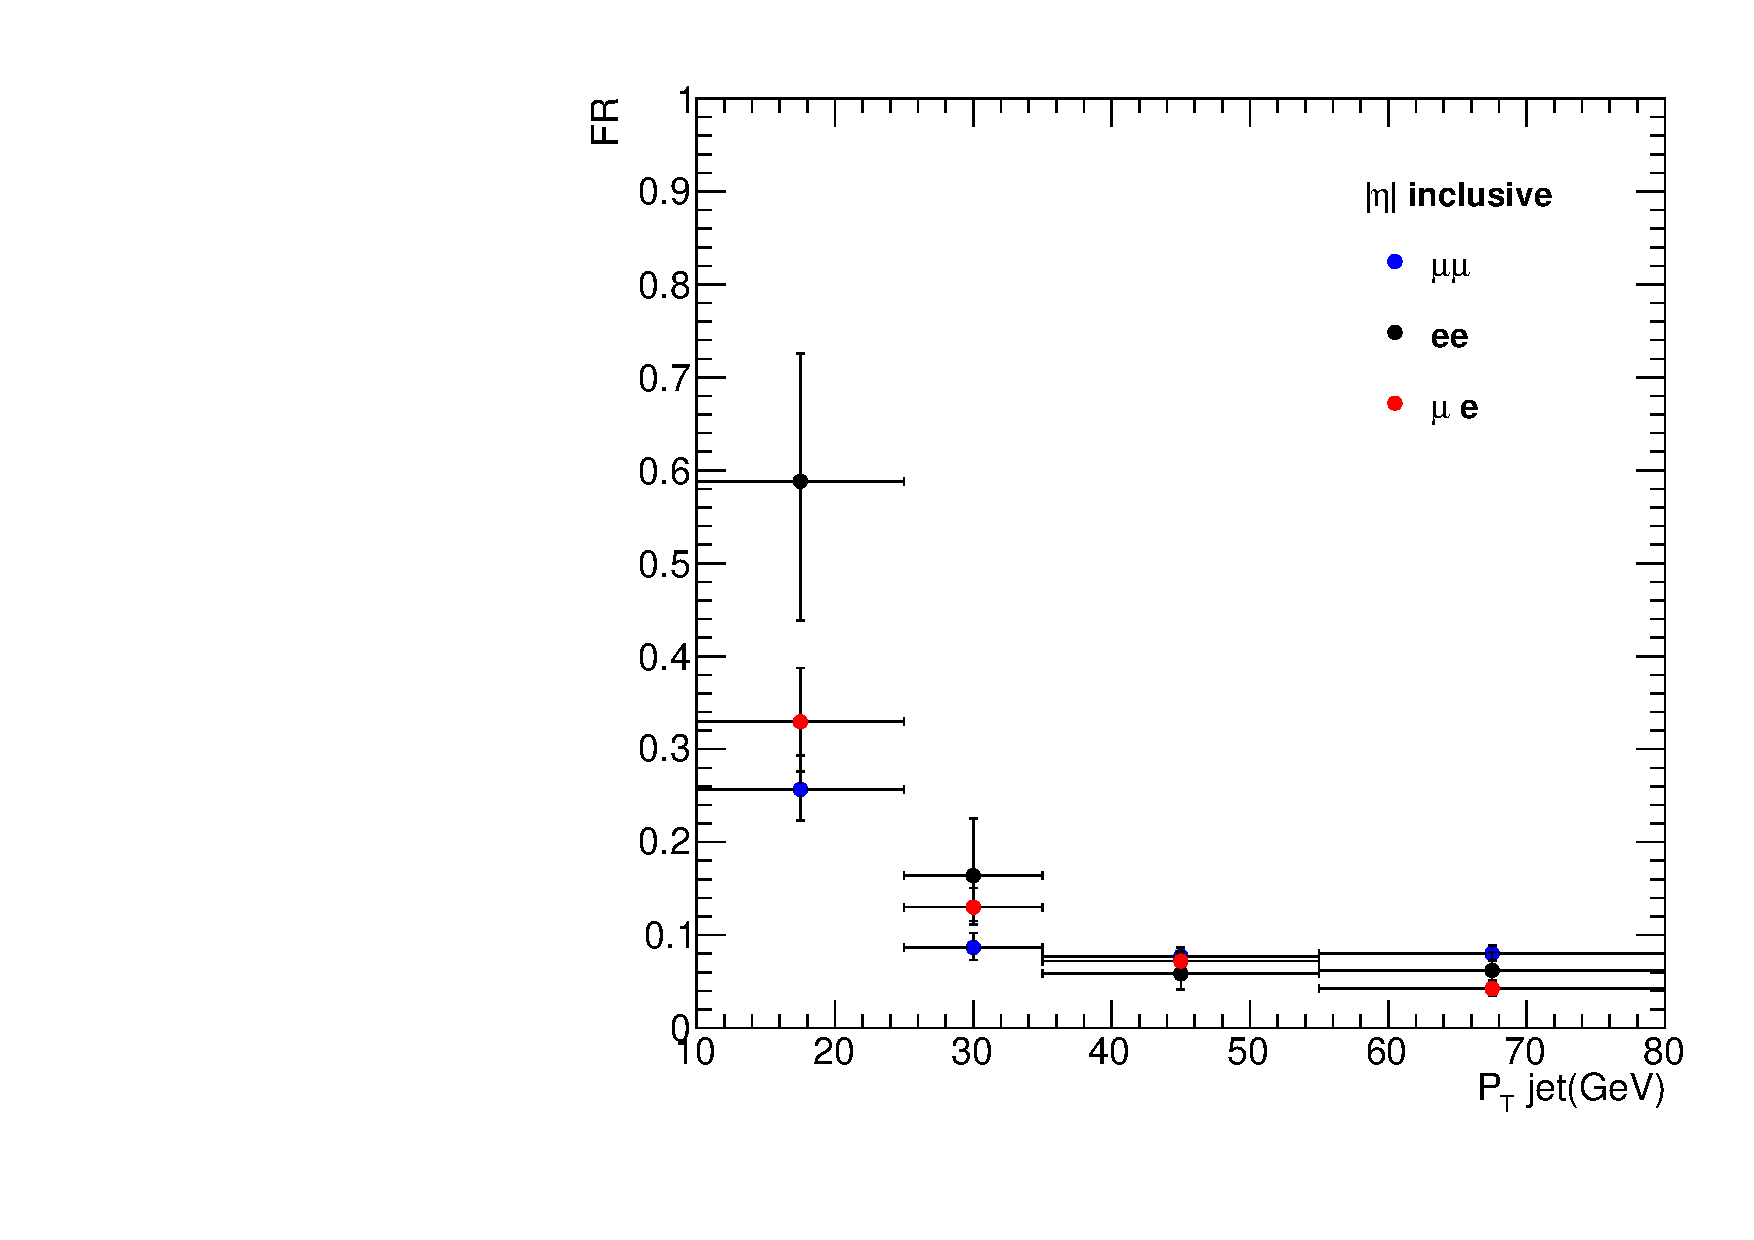
\includegraphics[width=.33\textwidth]{Figures/c6/backgrounds/FR/dFR/17/c_LeptonPt___eta_FR1.pdf}
  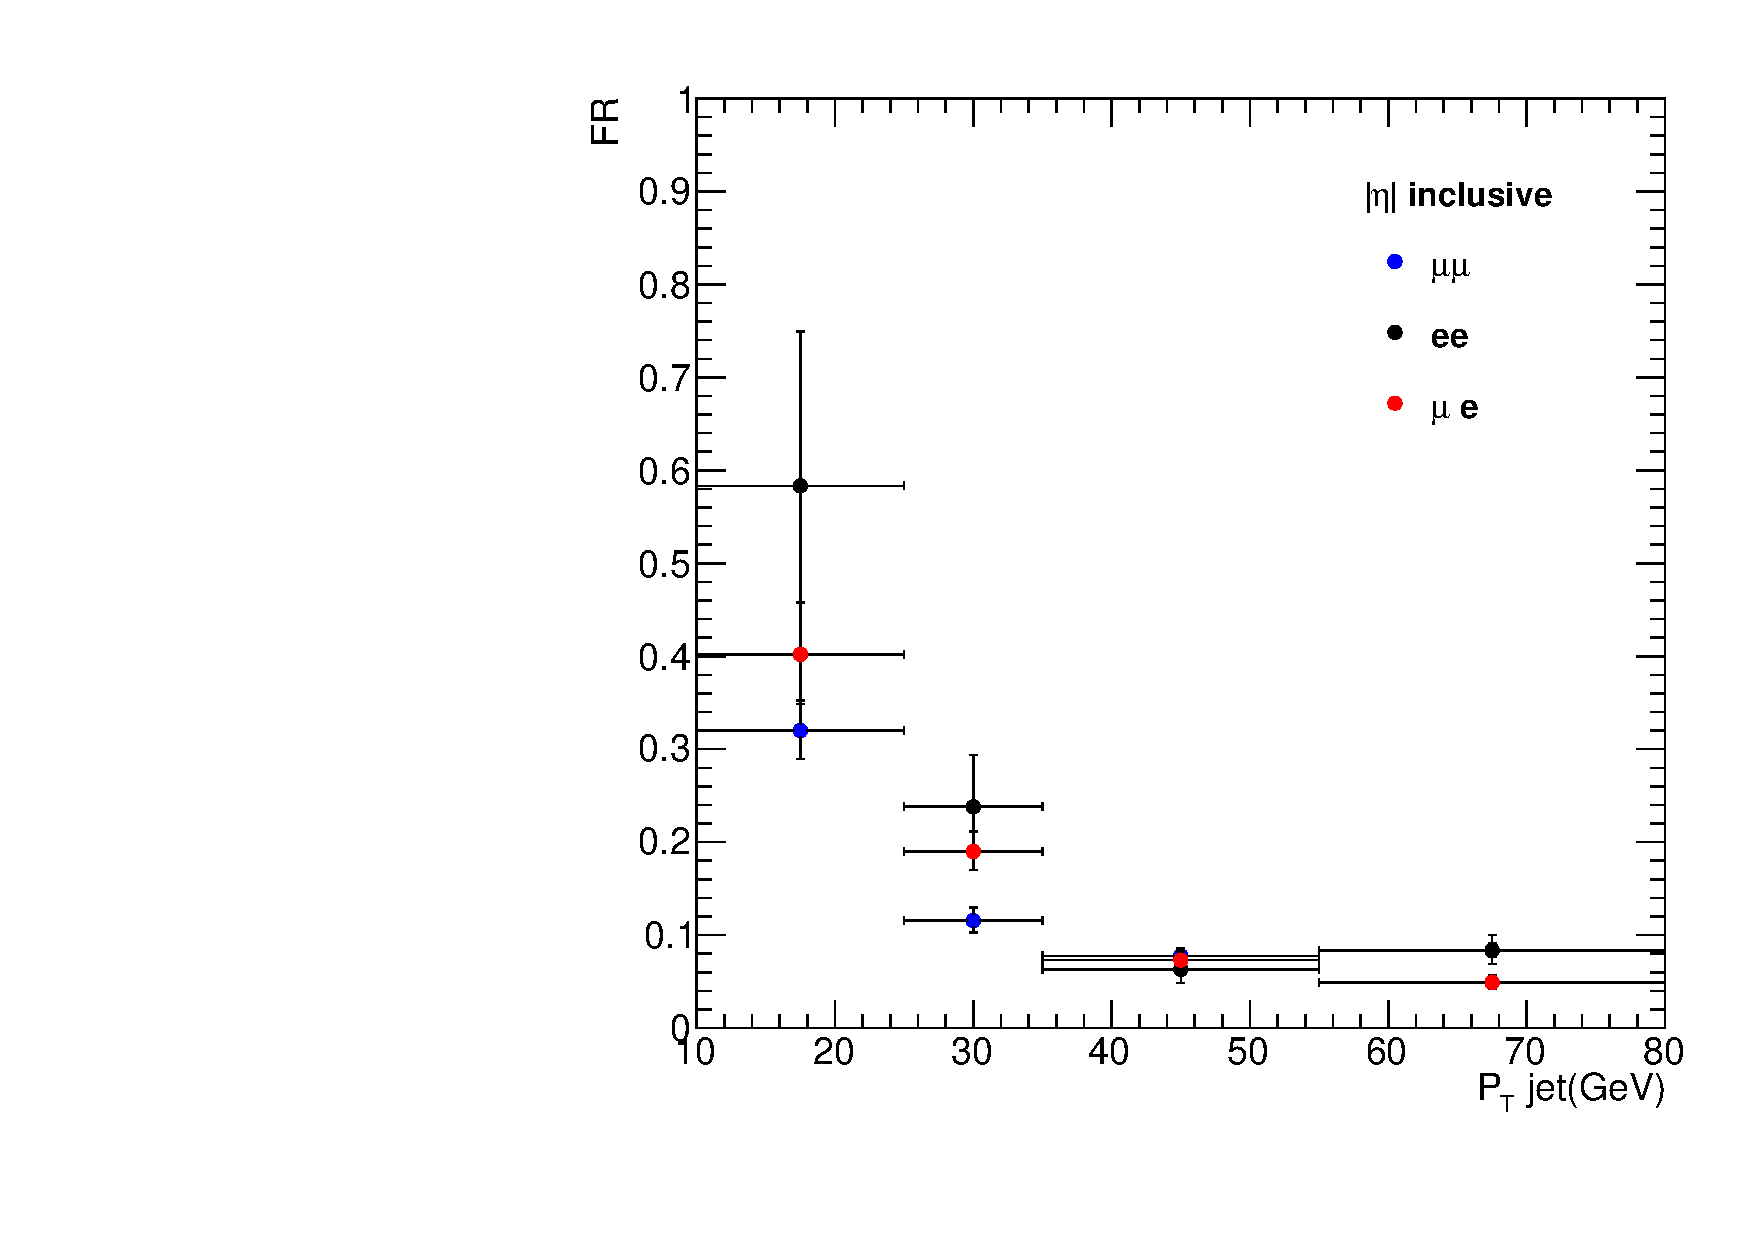
\includegraphics[width=.33\textwidth]{Figures/c6/backgrounds/FR/dFR/18/c_LeptonPt___eta_FR1.pdf}}
  \noindent
\makebox[\textwidth]{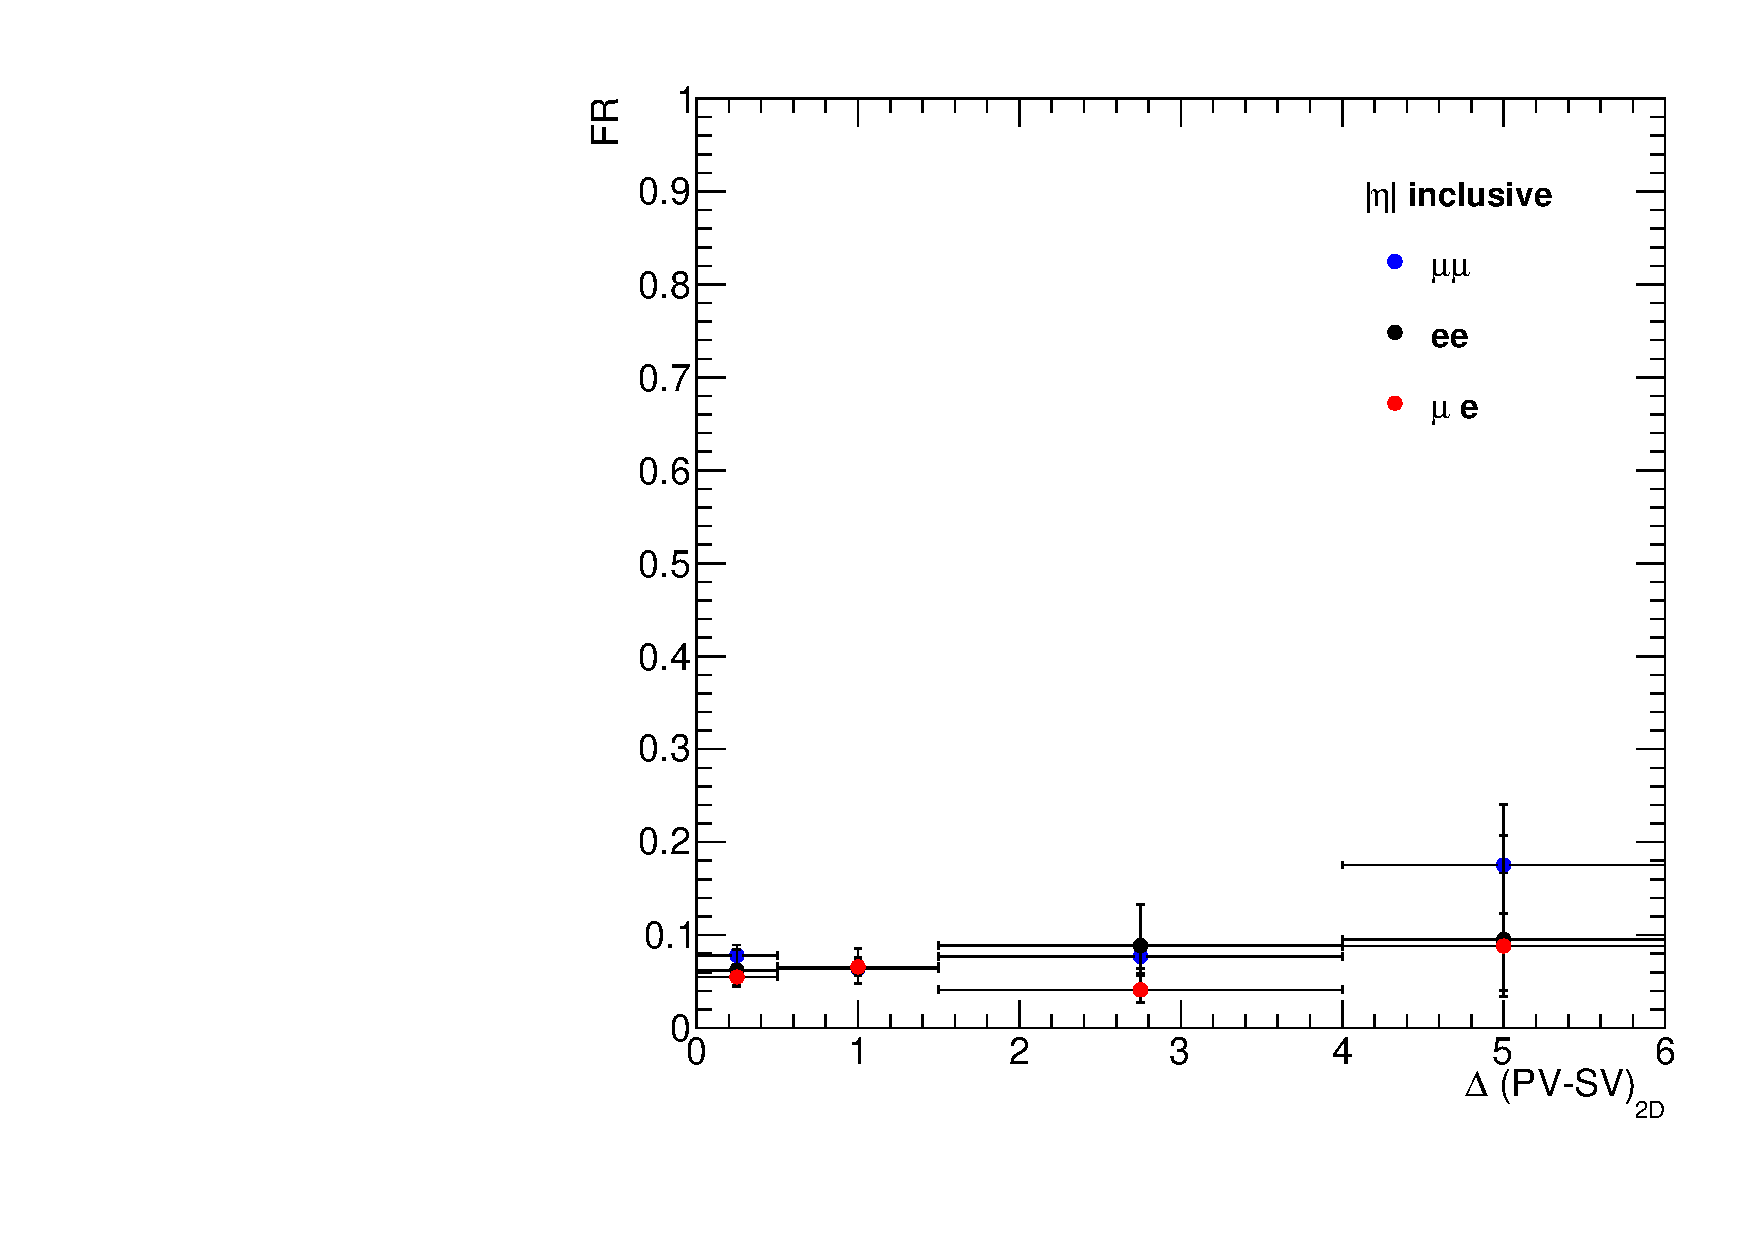
\includegraphics[width=.33\textwidth]{Figures/c6/backgrounds/FR/dFR/16/c_displacement_SR___eta_FR1.pdf}
  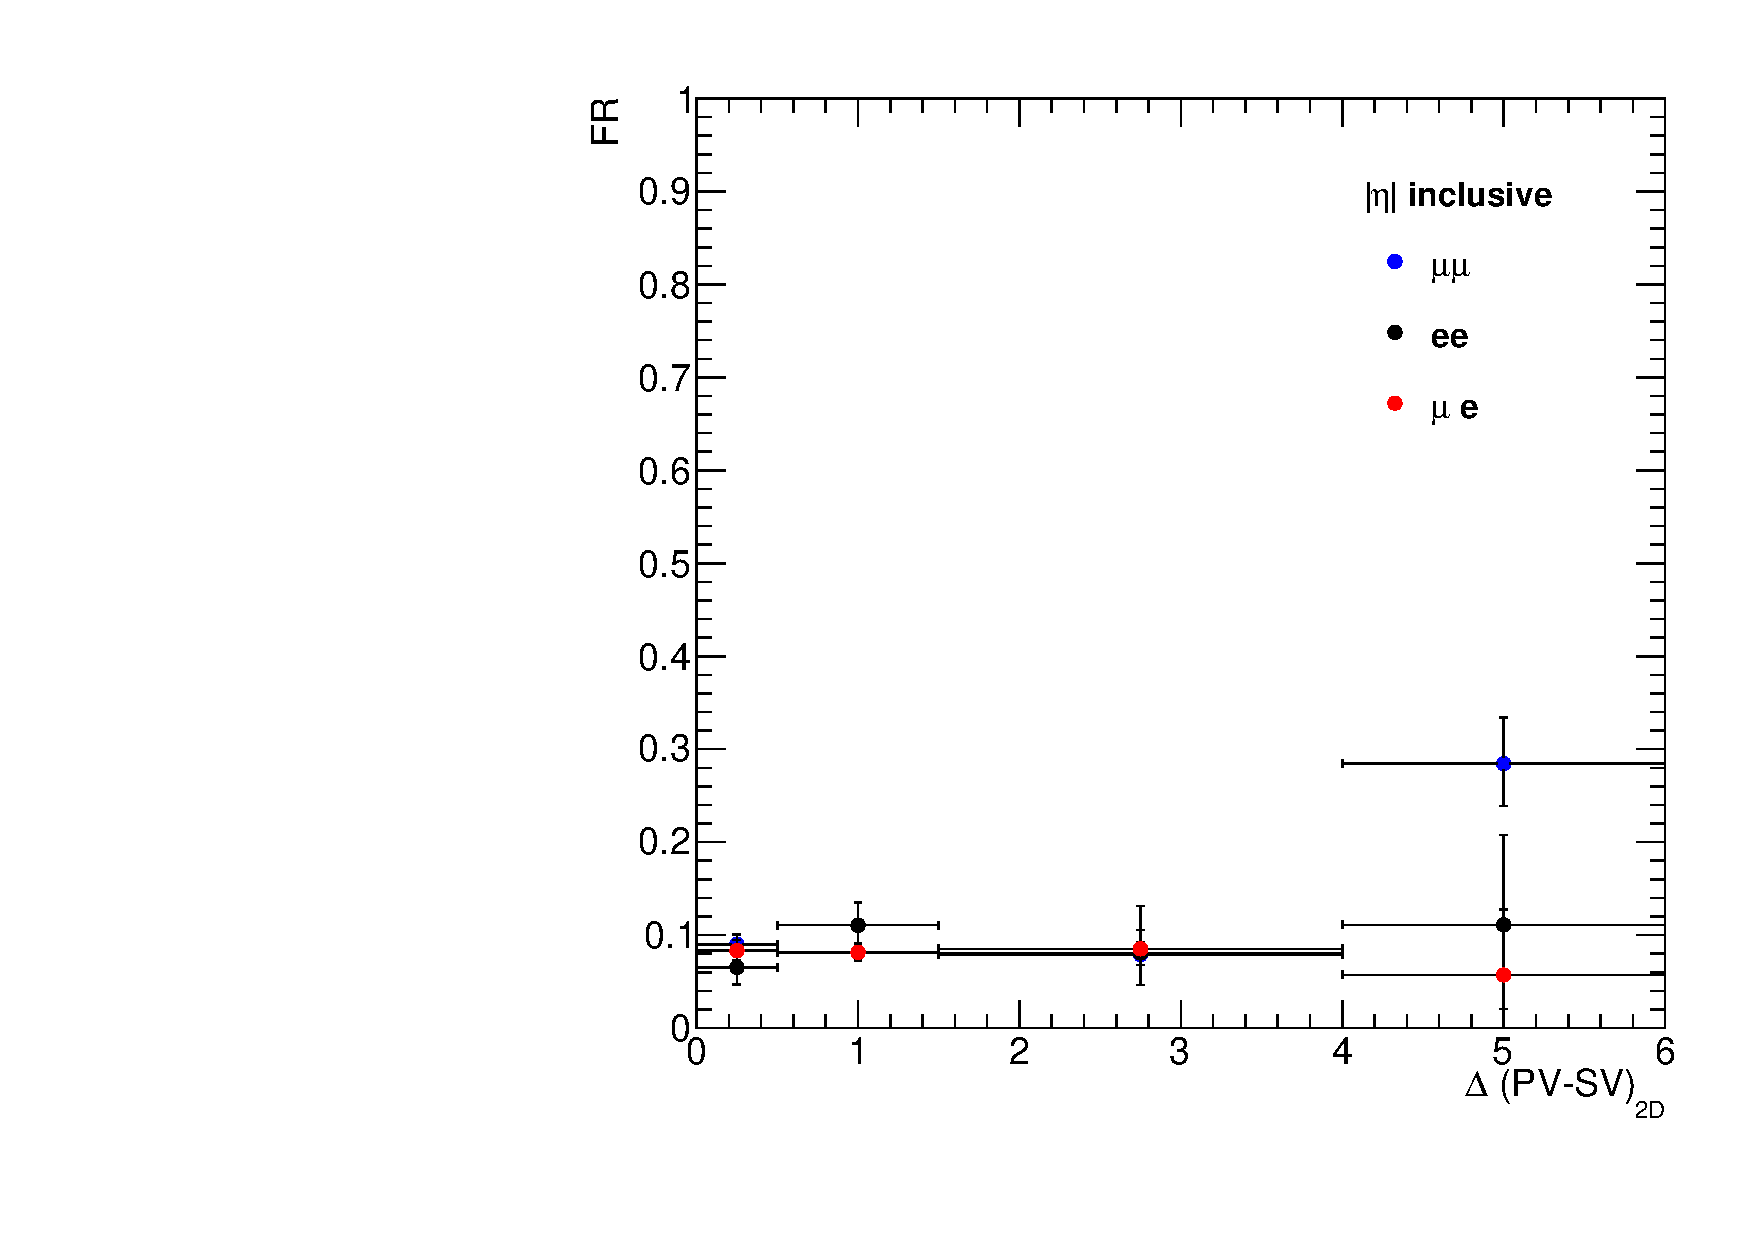
\includegraphics[width=.33\textwidth]{Figures/c6/backgrounds/FR/dFR/17/c_displacement_SR___eta_FR1.pdf}
  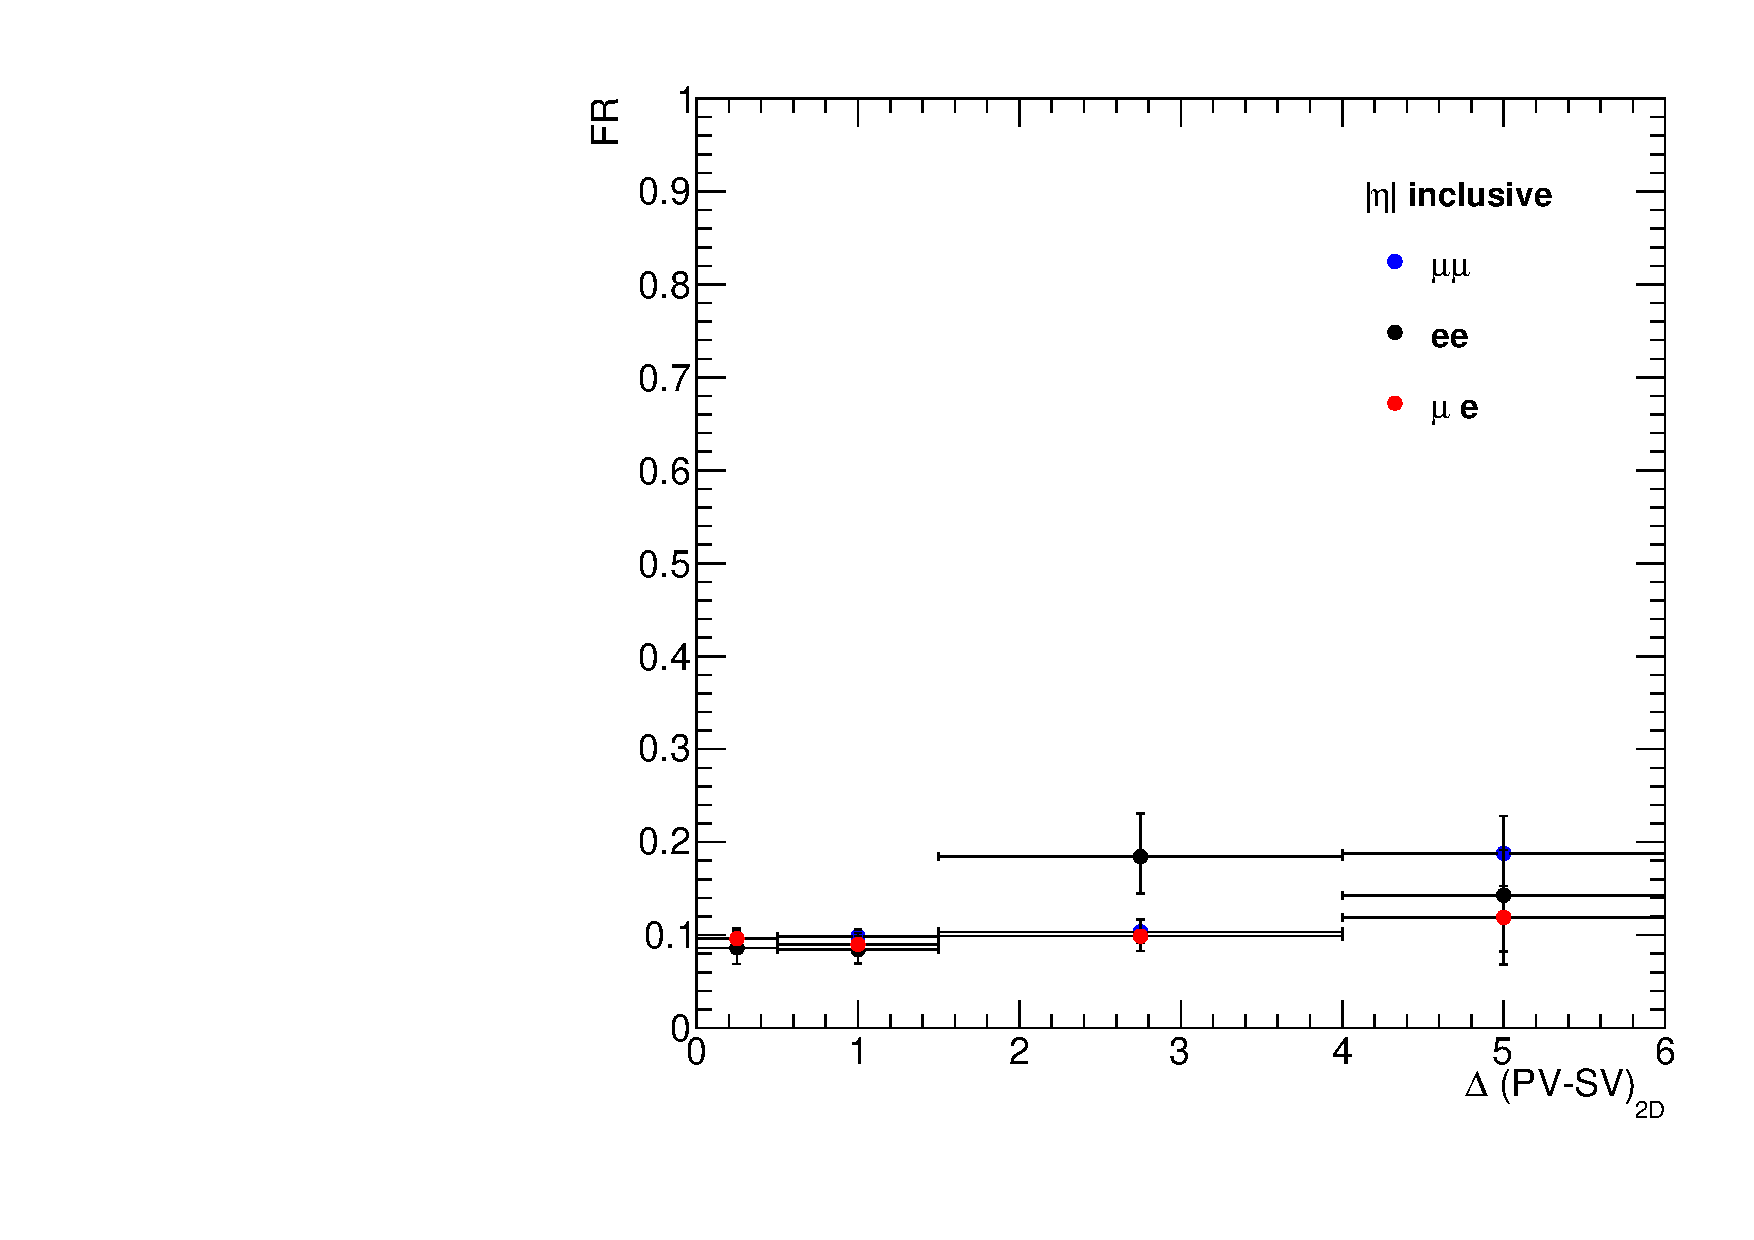
\includegraphics[width=.33\textwidth]{Figures/c6/backgrounds/FR/dFR/18/c_displacement_SR___eta_FR1.pdf}}
  \caption{\Dfr (\dfr) measured in 2016/17/18 (left,
    middle, right) data as a function of \ptj (top) and \Deltwod (bottom),
    for events with two electrons (black), with
    an electron and a muon (red), and with two muons (blue).}
  \label{fig:dFR_ptjet_16}
\end{figure}

The application region for double-fake lepton backgrounds 
is defined using the same selection as the signal region (see
Table~\ref{tab:baselinesel}), but with one or two \fo -non-\tD
leptons that either be associated to the same jet or have $\DR<0.45$. 
The background from double-fake leptons in the signal region is
estimated from the event yields in the application region using
the formula
\begin{linenomath}
  \begin{equation}
    \label{eq:dFRbkg}
    N_{\mathrm{double\: fakes}}^{\mathrm{sig}} ~=~ 
    \sum_i\frac{\dfr(\ptjs{i})}{1-\dfr(\ptjs{i})}\;,
  \end{equation}
\end{linenomath}
where the sum runs over all the events in the application region, with jet transverse momentum \ptjs{i}.
\subsubsection{Estimation of single-fake background}
\label{sec:singleFakeBkg}

The measurement of the single-fakerate (\fr), \sfr background follows the exact same
procedure as the one explained in Section~\ref{sec:singleFR}. Thus, to
avoid repetitions, only the final measured \fr are presented here.

Figure~\ref{fig:sfr_data} shows the measured
values of \sfr for electrons and muons in simulation and in data,
respectively, as a function of \ptc and in different \abseta bins.
\begin{figure}[h!]
  \centering
  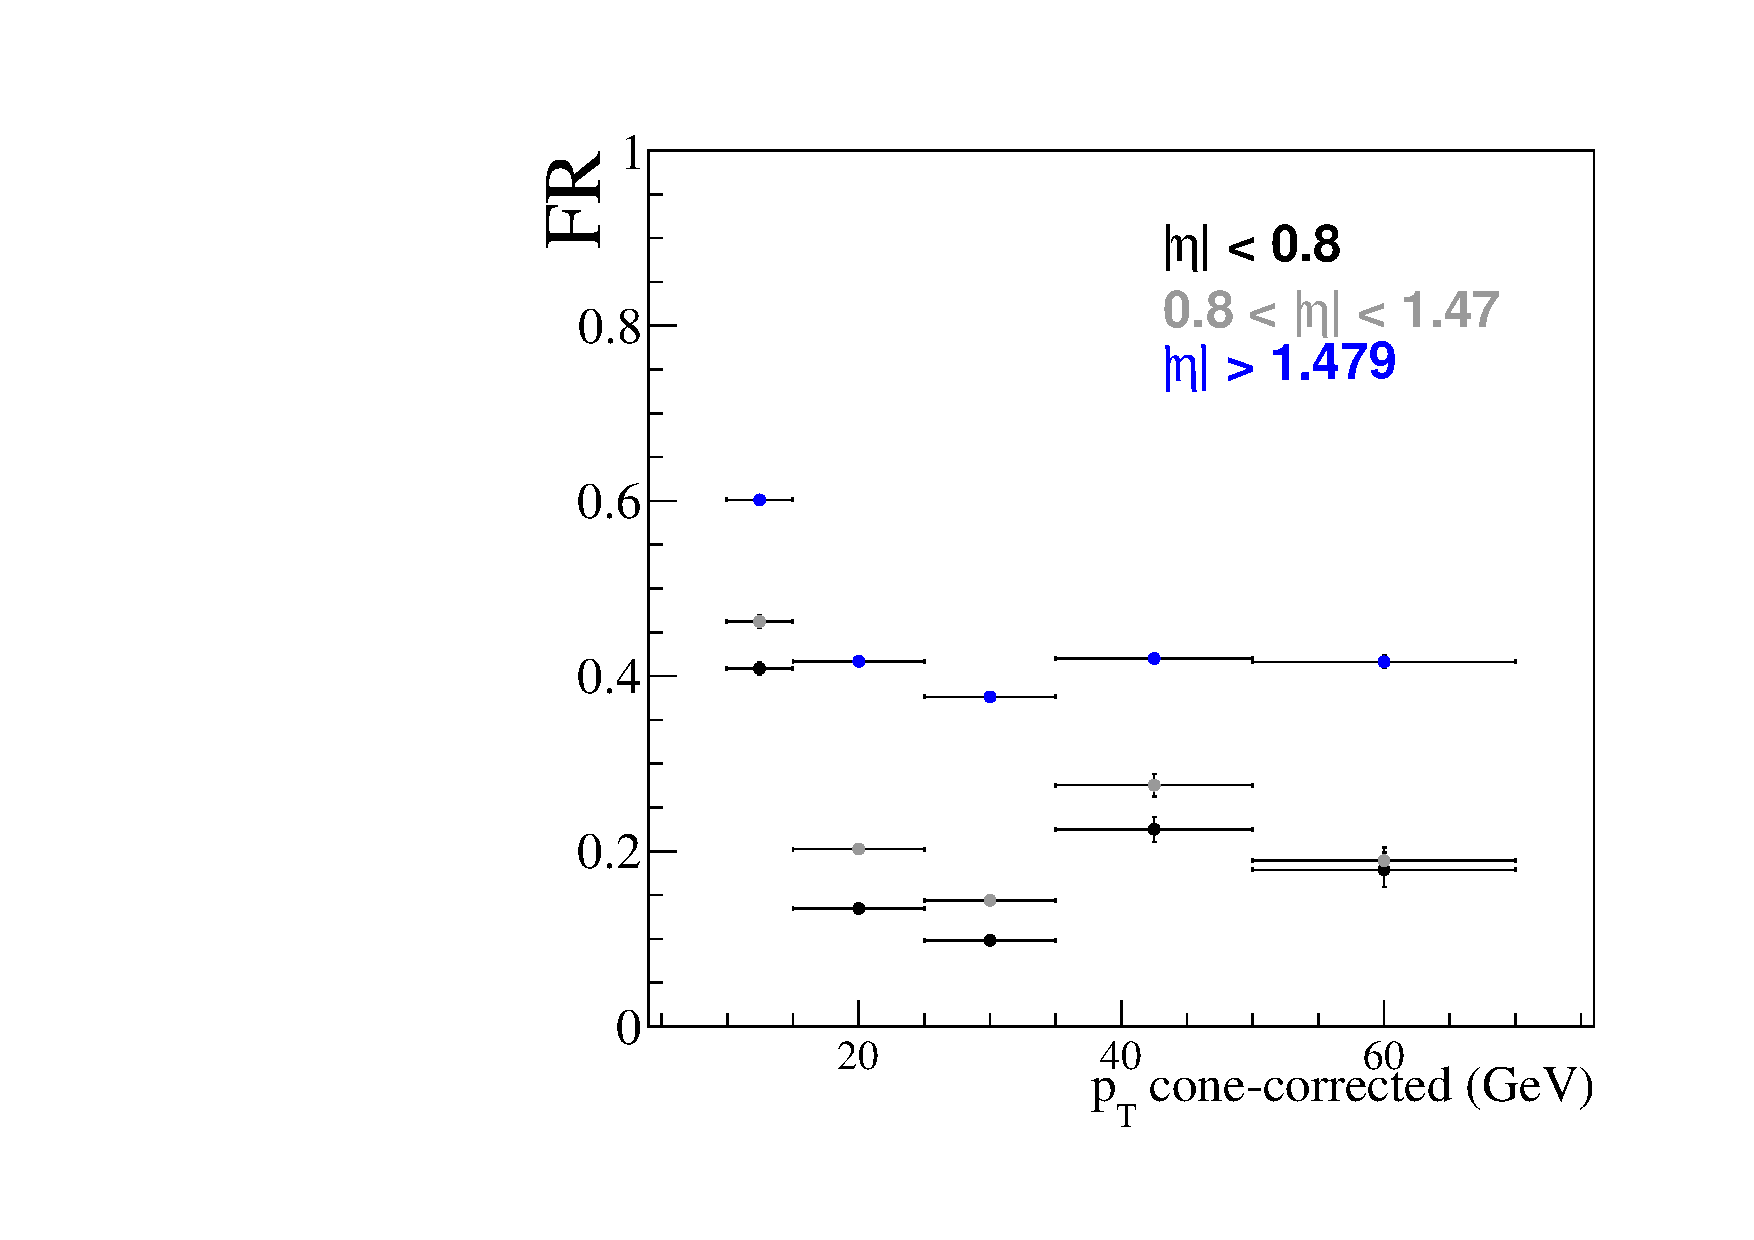
\includegraphics[height=5cm, width=5.4cm]{Figures/c6/backgrounds/FR/sFR/data/electrons.pdf}
  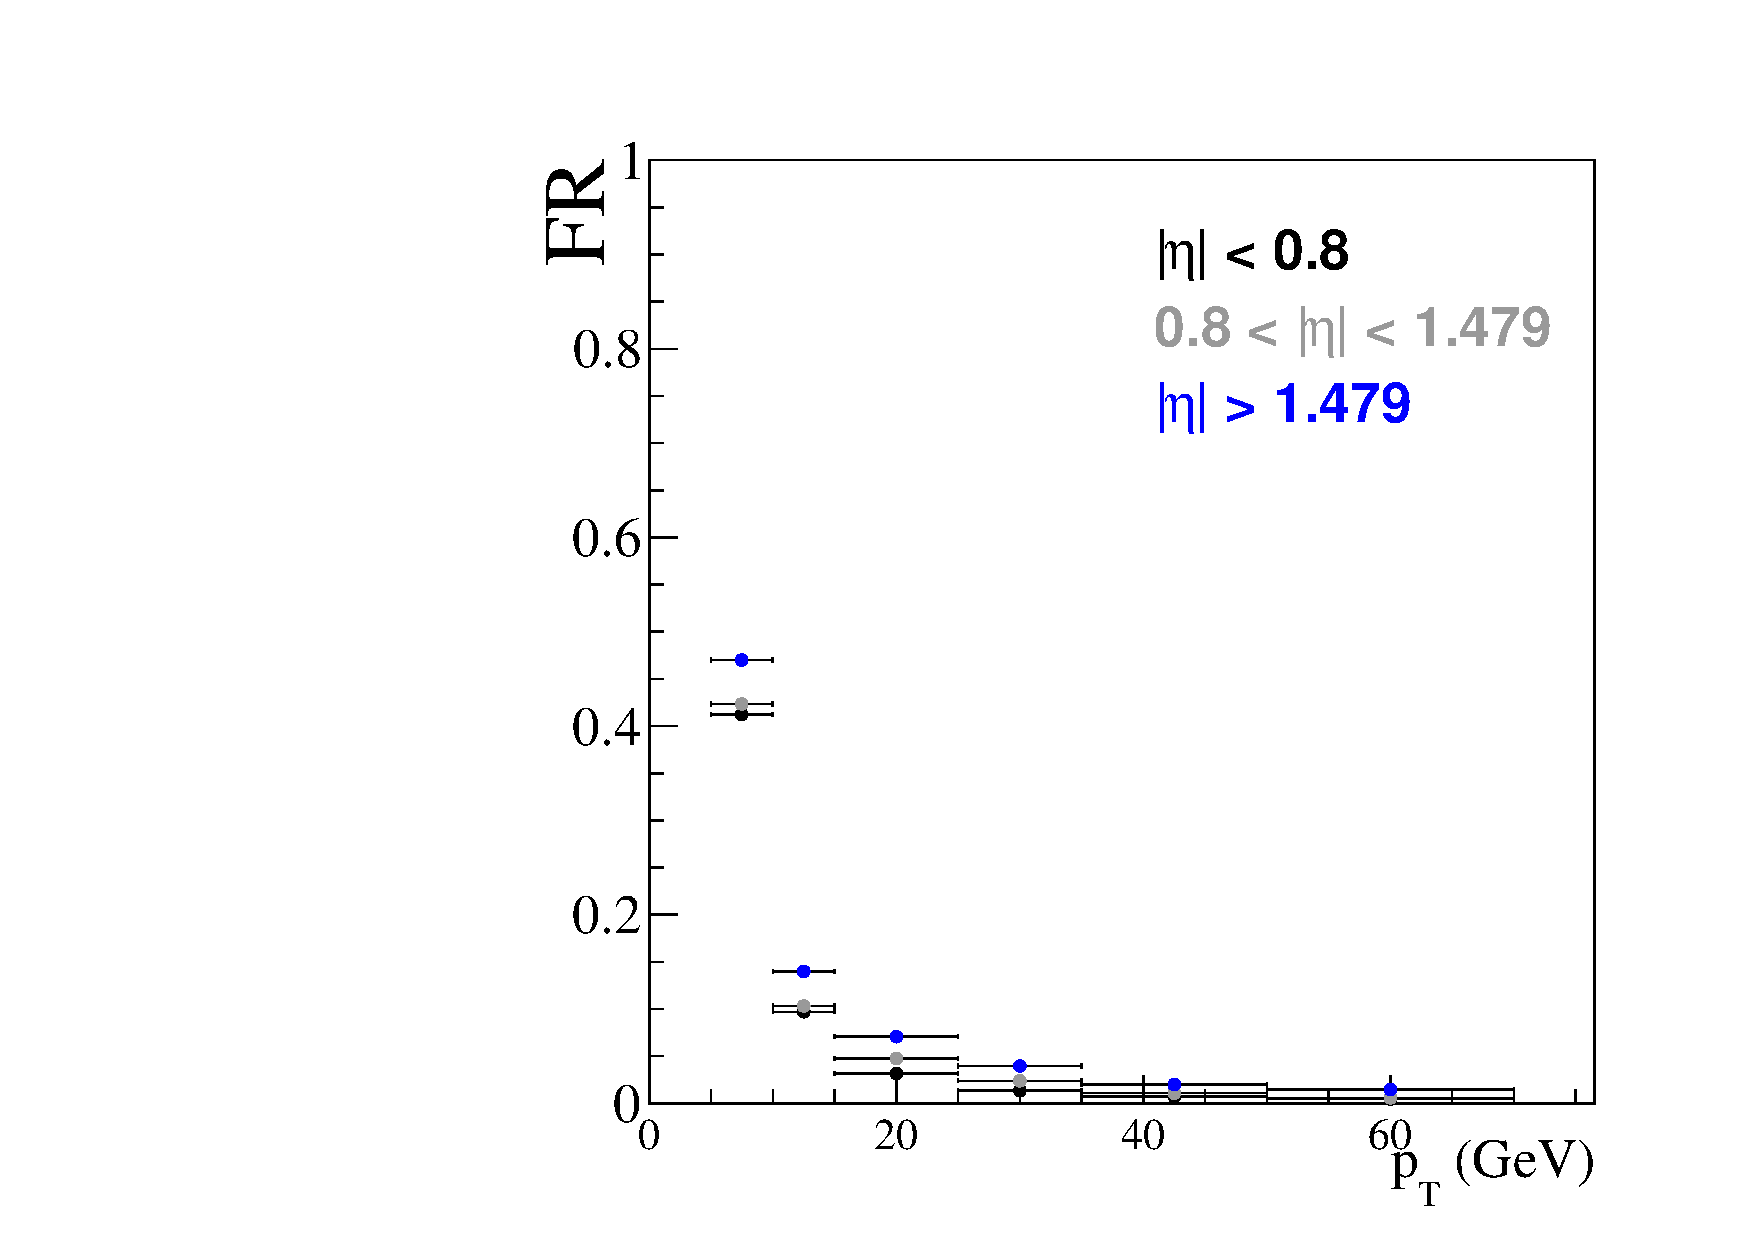
\includegraphics[height=5cm, width=5.4cm]{Figures/c6/backgrounds/FR/sFR/data/muons.pdf}\\
  \caption{\fr (\sfr) measured in 2016 data for electrons (left) and
    muons (right) as a function of \ptc, for \abseta ranges $[0,0.8]$, $[0.8,1.479]$, and $[1.479,2.5]$.}
  \label{fig:sfr_data}
\end{figure}

Several studies in simulation are performed to ensure that different origins of fake leptons lead to
similar \fr values (refer to Section~\ref{sec:tight_loose_method} for
all the detailed motivations). To good extend no strong dependence on
\dxy is
observed as well as for different origins of fake leptons. Thus, the 
the parametrization of the \sfr is made to depend only on \ptc and \abseta and the
dependence on \dxy is ignored. 
Figure~\ref{fig:sfr_dxy} shows that \sfr values are fairly independent
of the lepton \dxy which is used as proxy for the displacement. 

\begin{figure}[h!]
  \centering
  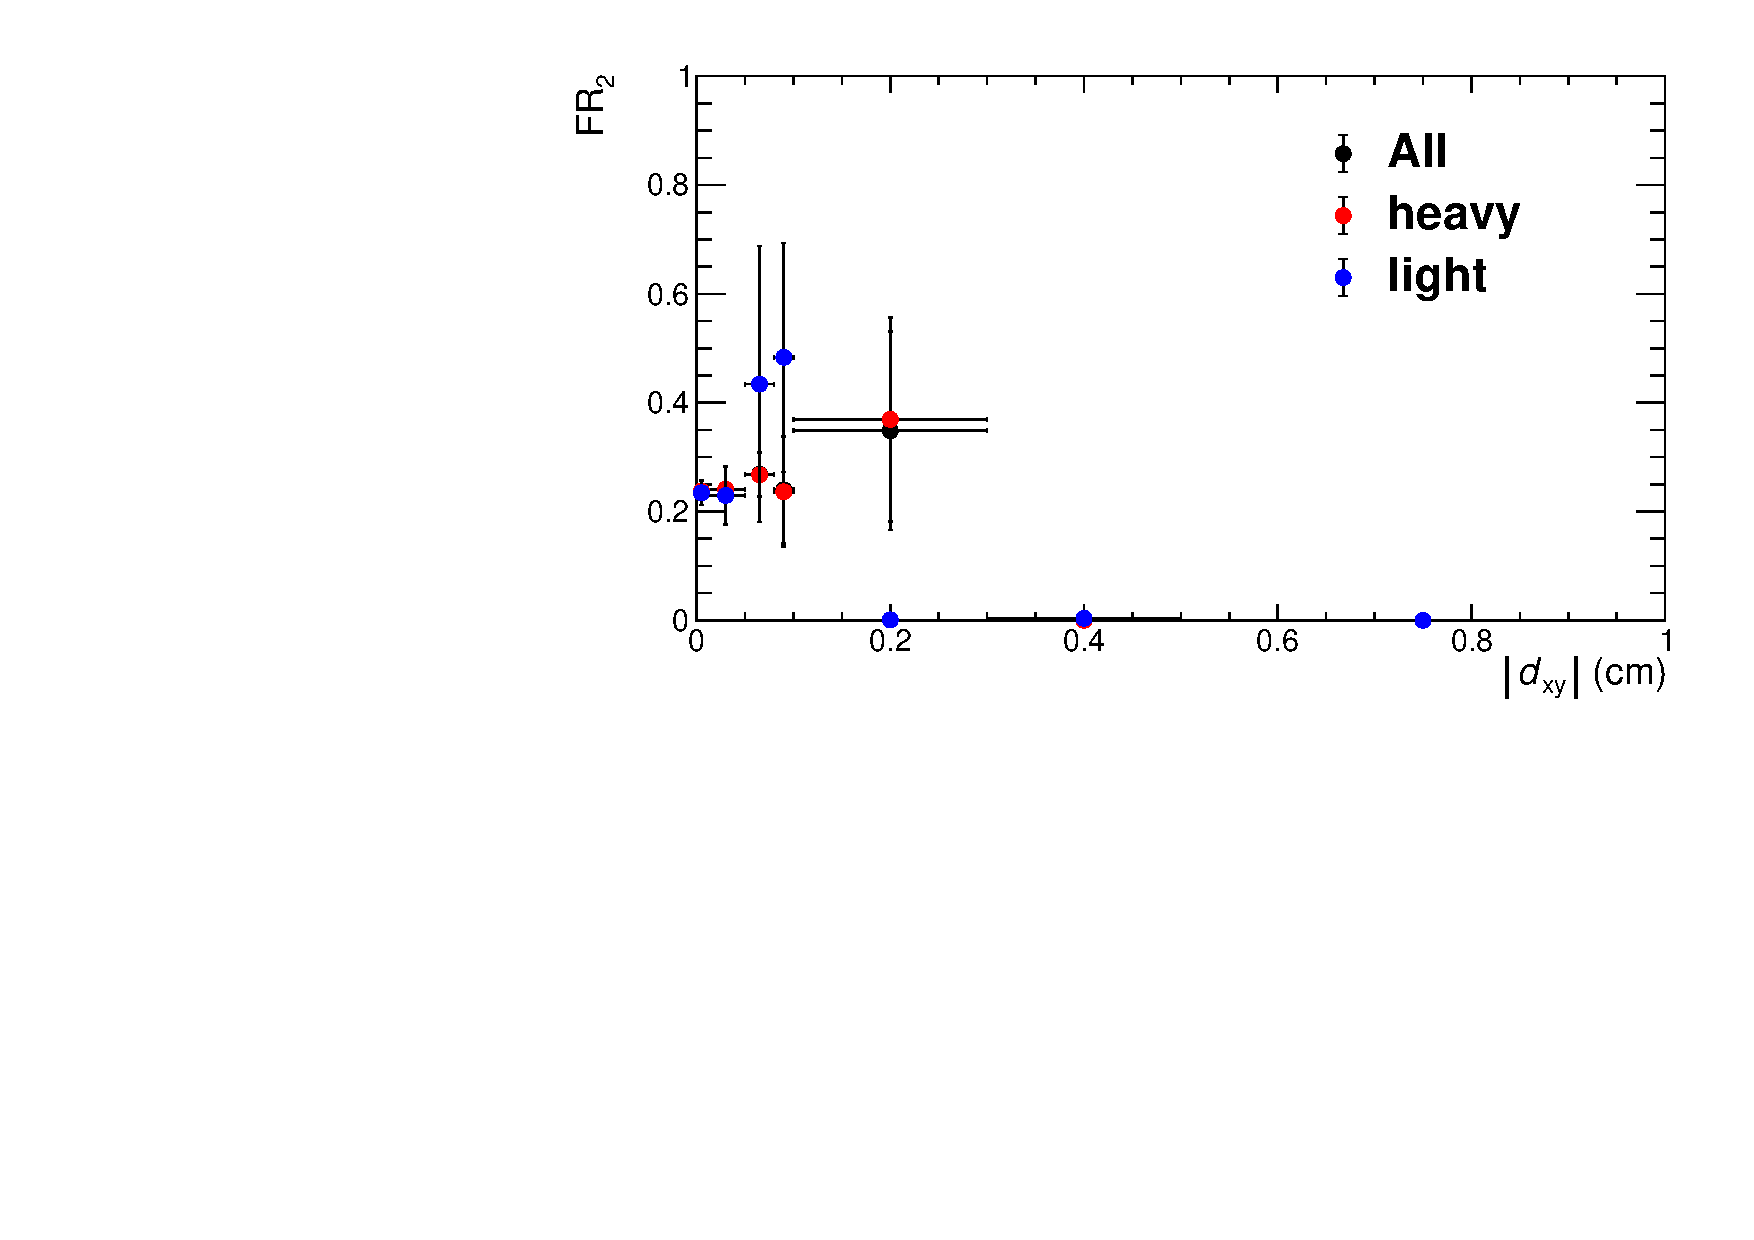
\includegraphics[width=.32\textwidth]{Figures/c6/backgrounds/FR/sFR/QCD/dxy_ele_eta1_FR2.pdf}
  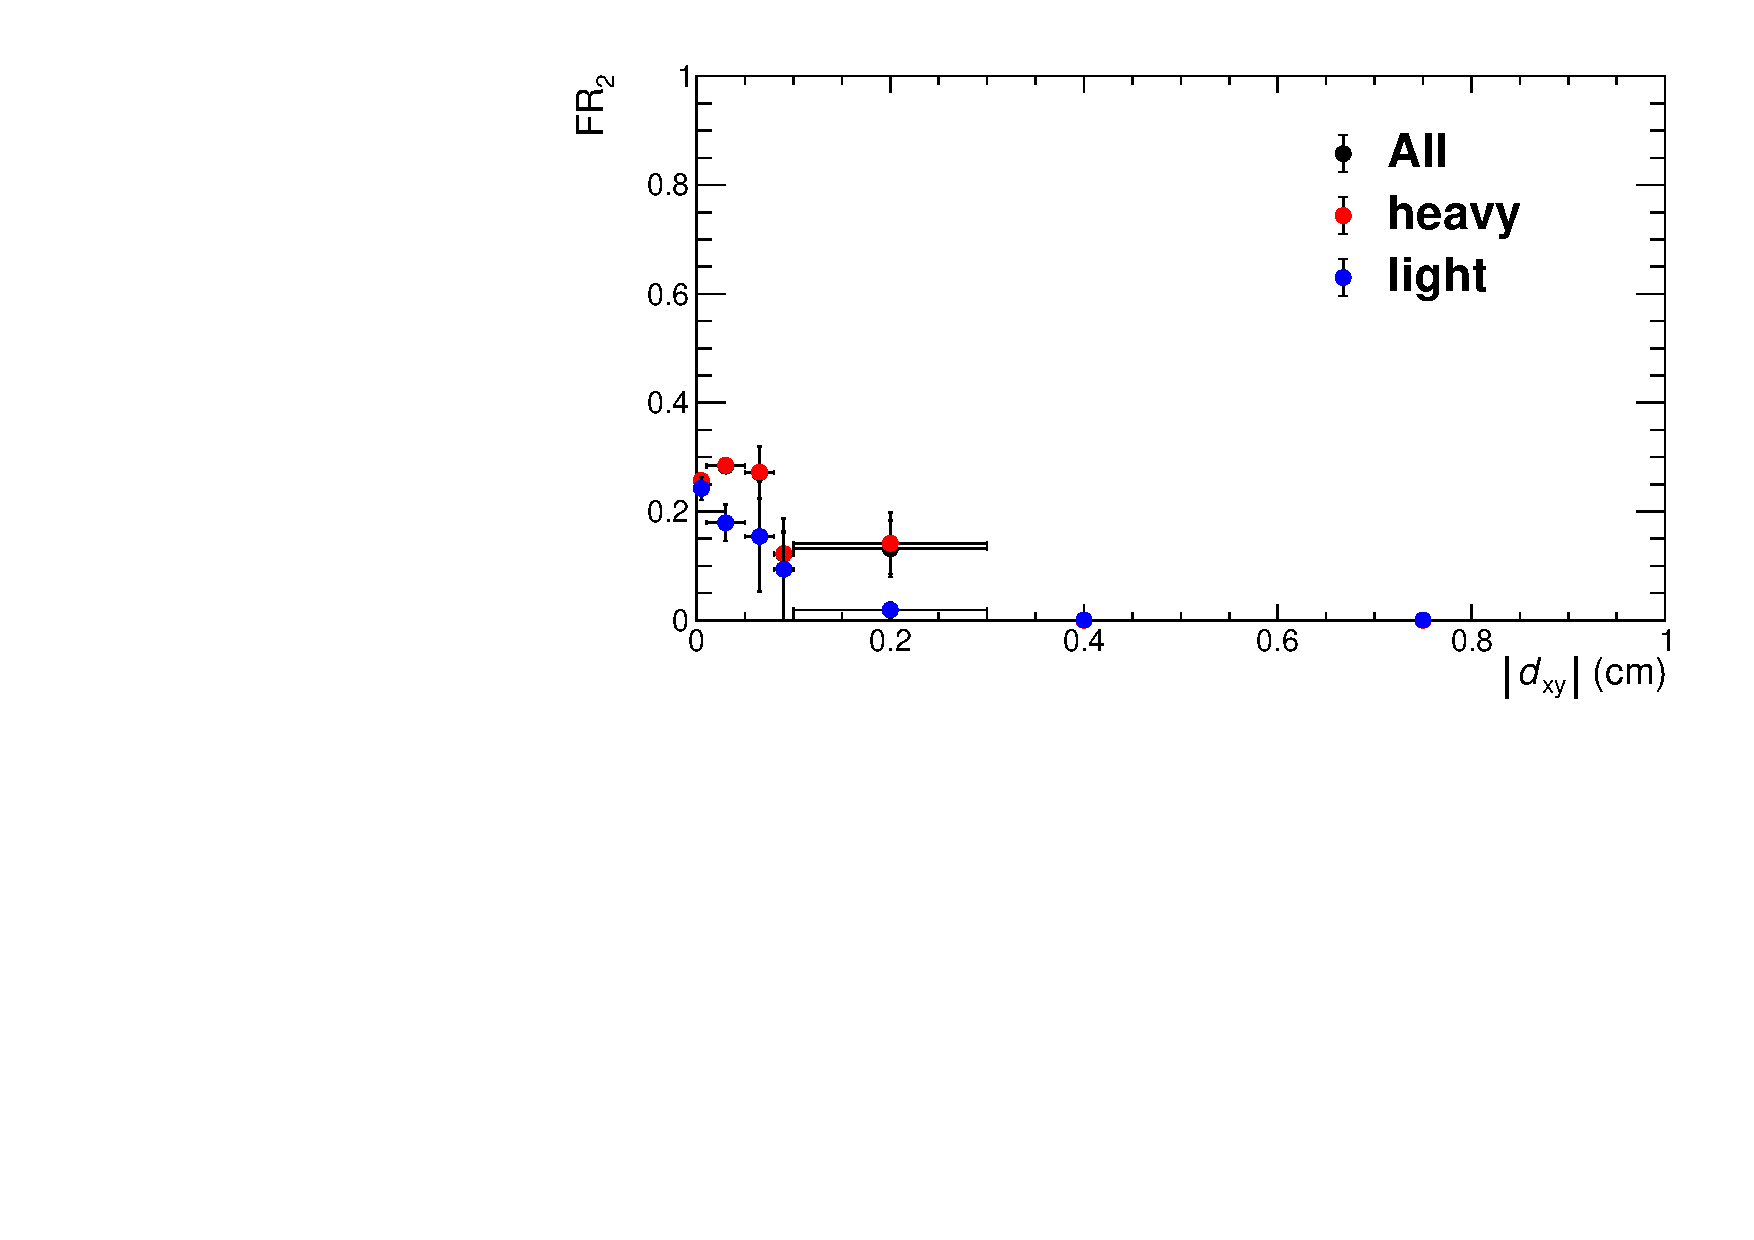
\includegraphics[width=.32\textwidth]{Figures/c6/backgrounds/FR/sFR/QCD/dxy_ele_eta2_FR2.pdf}
  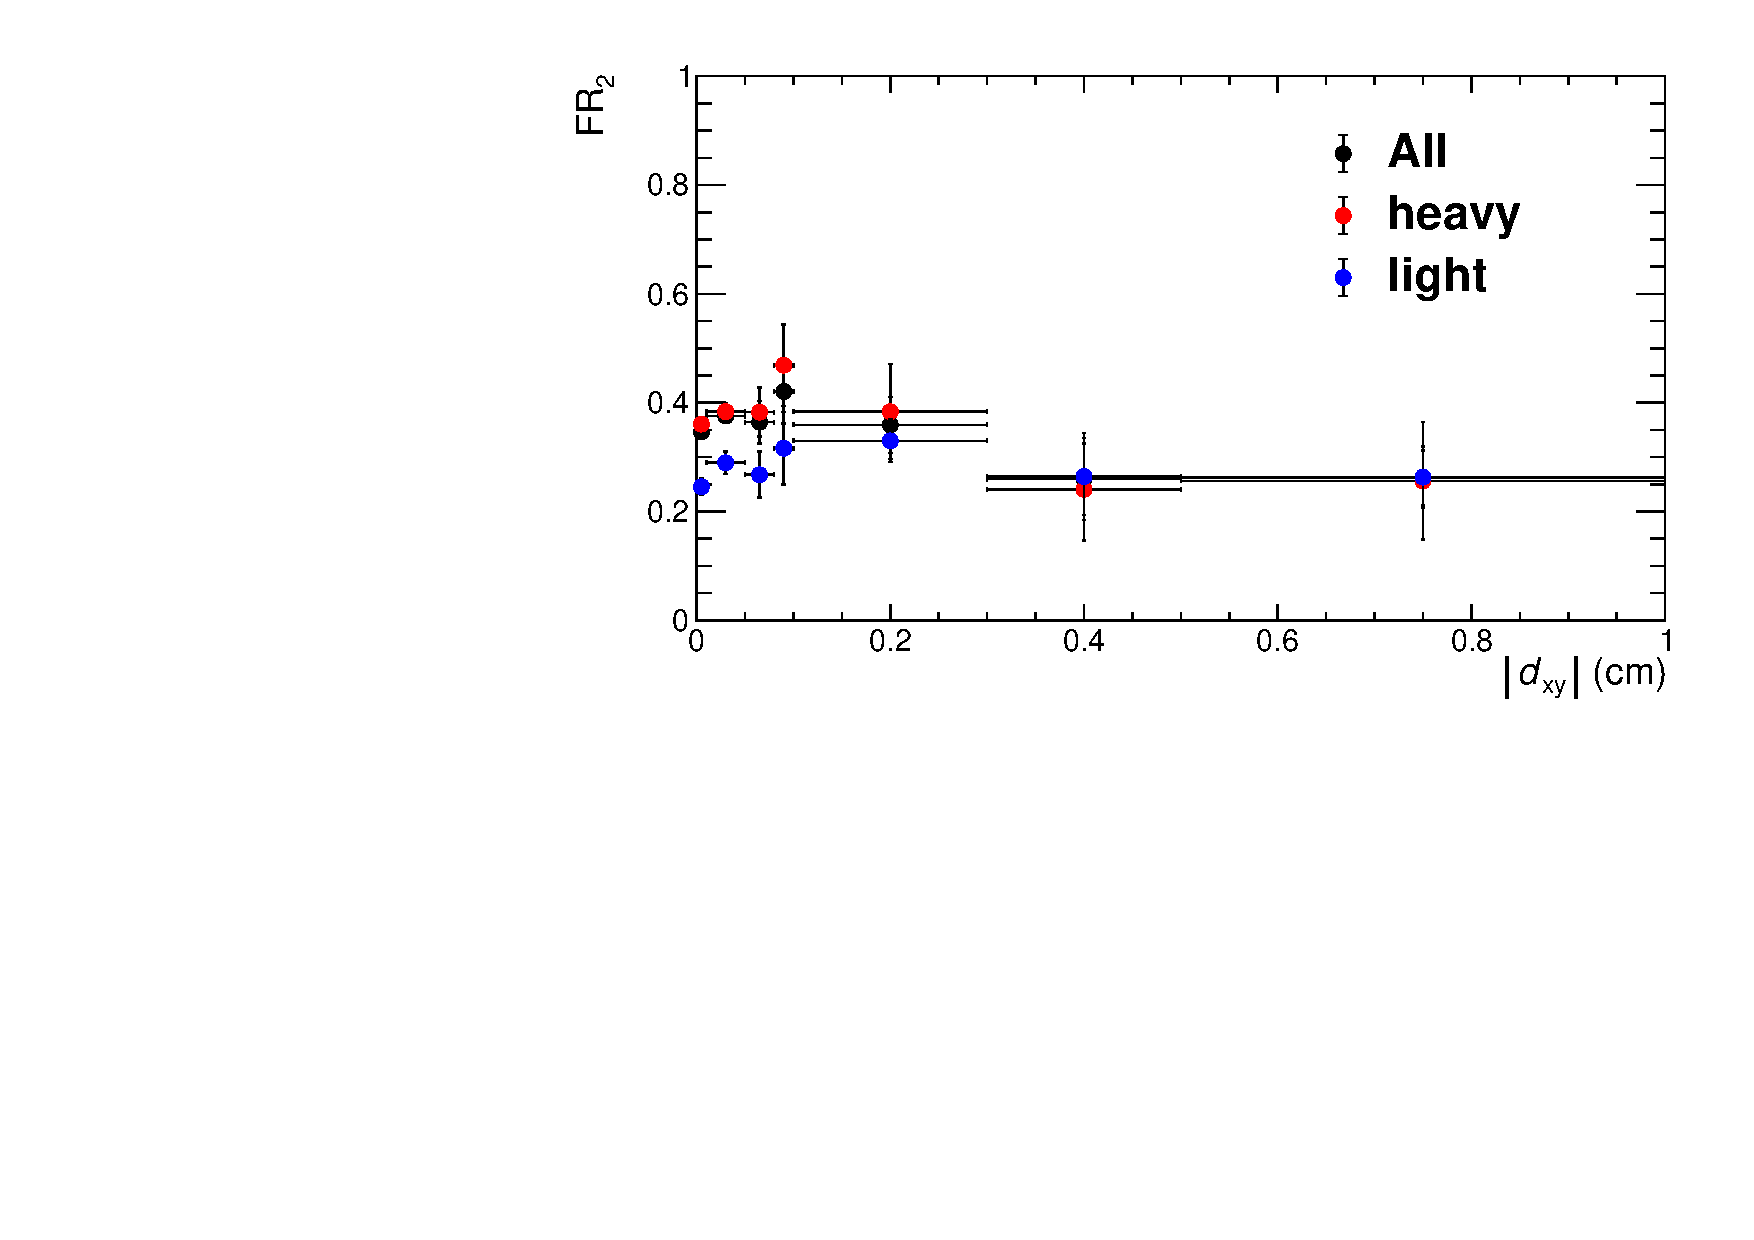
\includegraphics[width=.32\textwidth]{Figures/c6/backgrounds/FR/sFR/QCD/dxy_ele_eta3_FR2.pdf}\\
  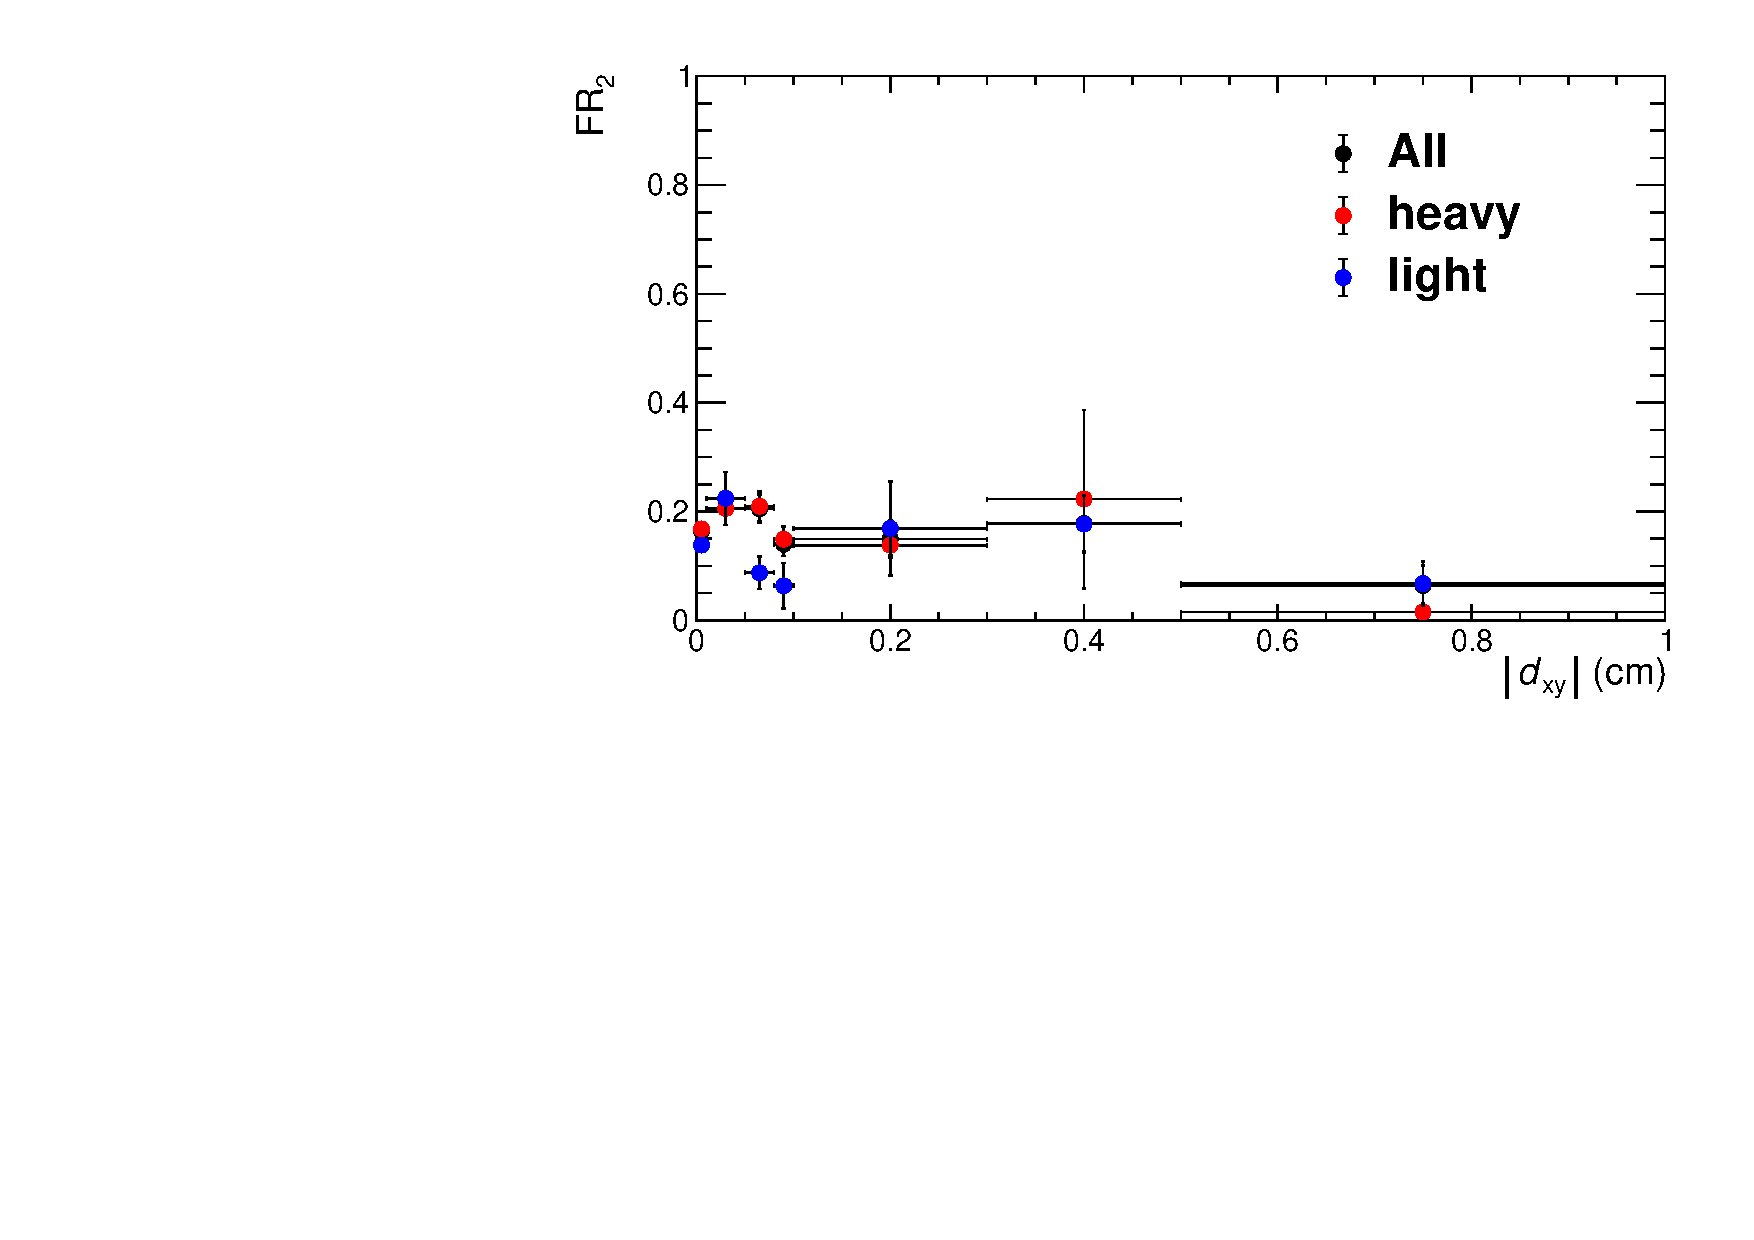
\includegraphics[width=.32\textwidth]{Figures/c6/backgrounds/FR/sFR/QCD/dxy_mu_eta1_FR2.pdf}
  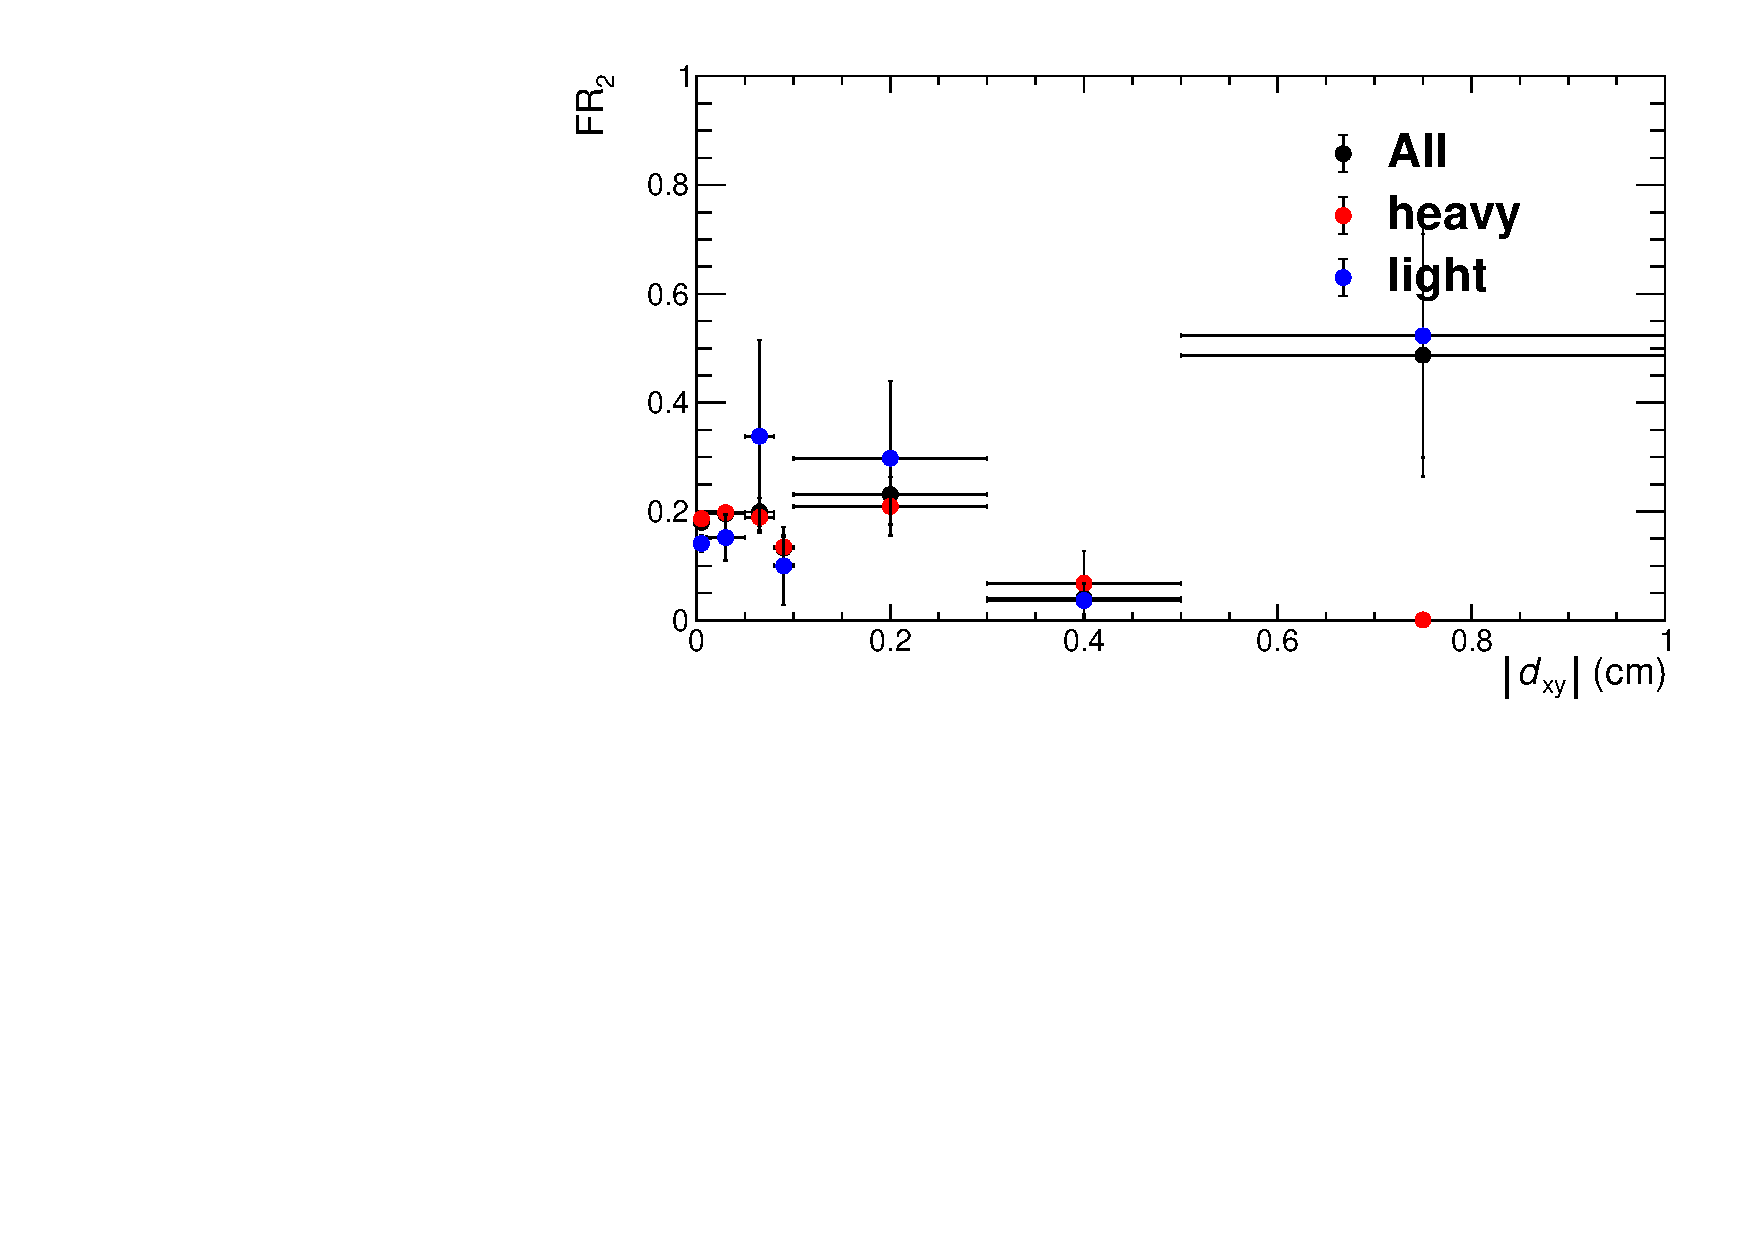
\includegraphics[width=.32\textwidth]{Figures/c6/backgrounds/FR/sFR/QCD/dxy_mu_eta2_FR2.pdf}
  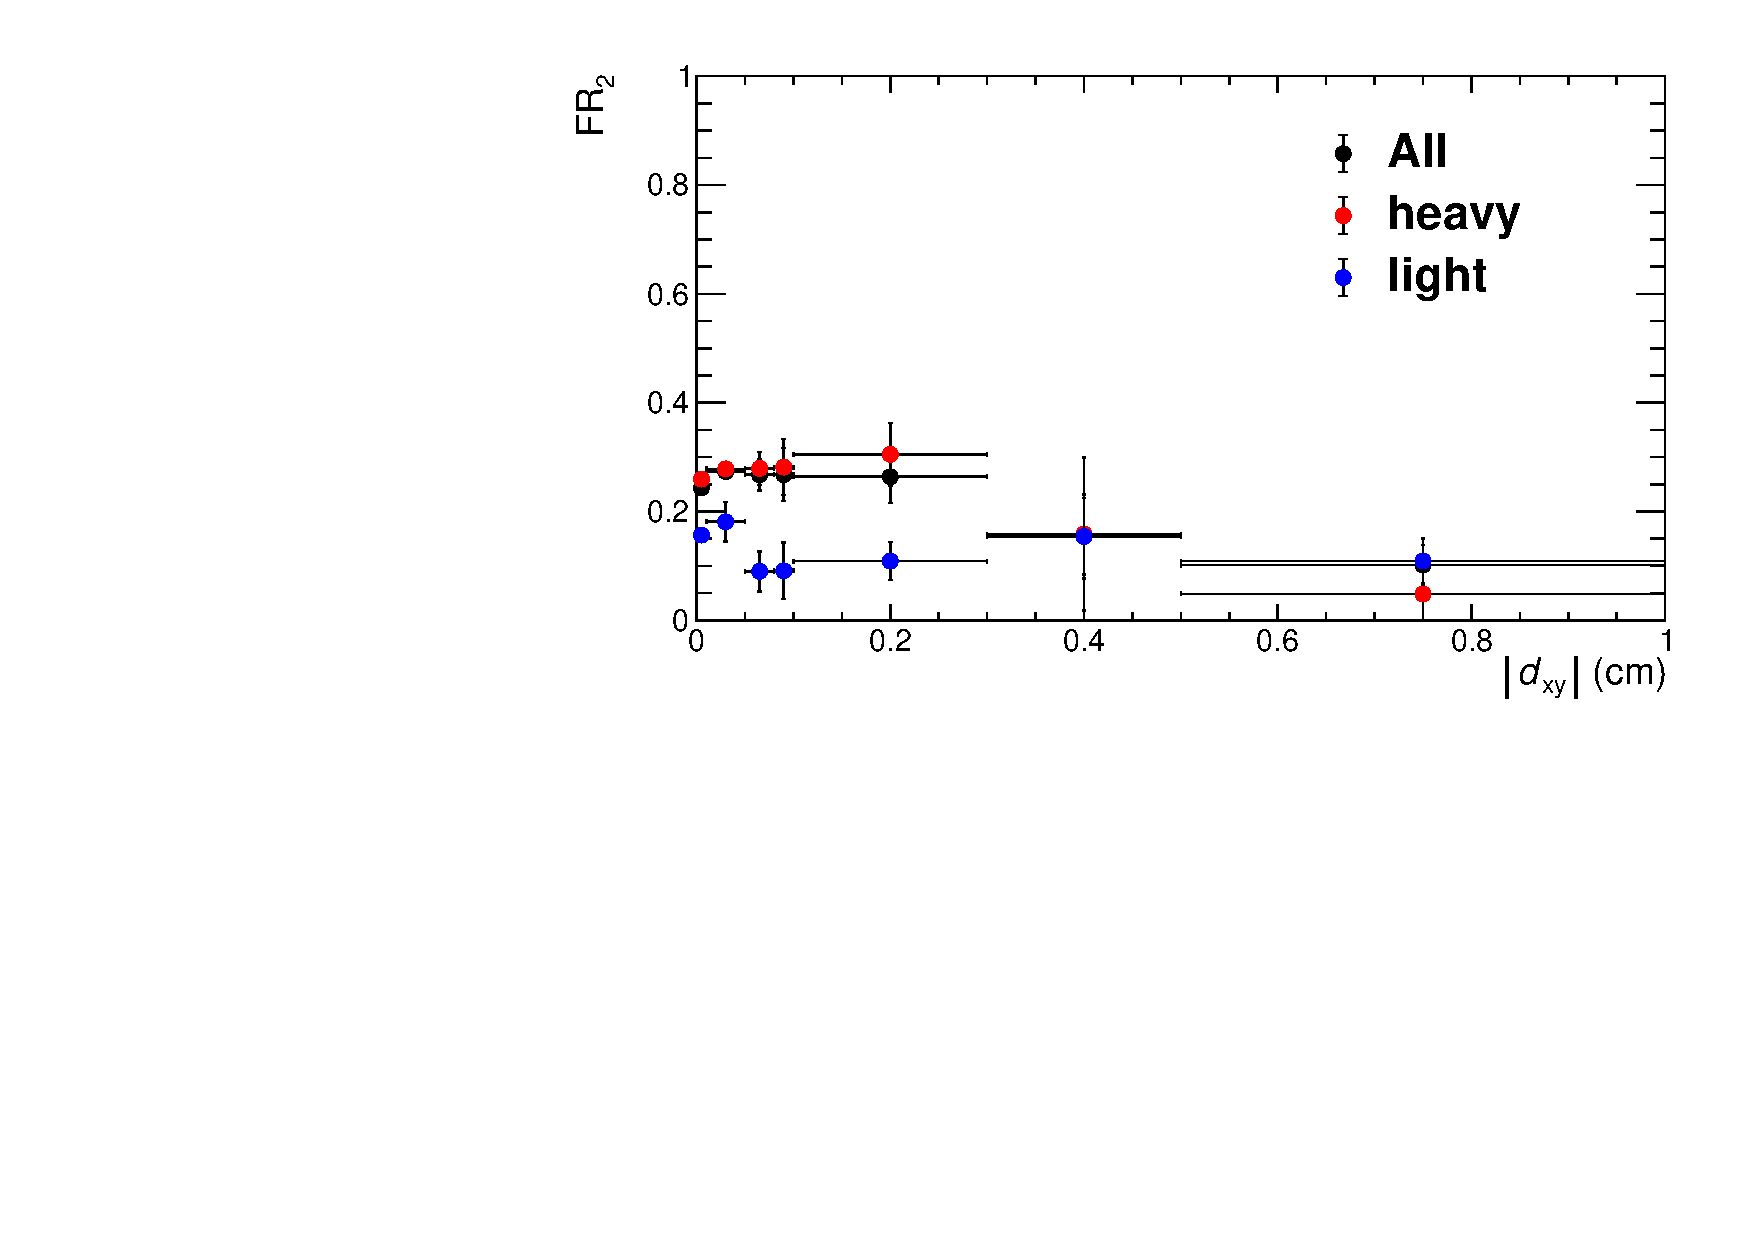
\includegraphics[width=.32\textwidth]{Figures/c6/backgrounds/FR/sFR/QCD/dxy_mu_eta3_FR2.pdf}
  \caption{Single fake rates obtained in 2016 simulation for electrons
    (top) and muons (bottom) as
    a function of \dxy, for \abseta ranges $[0,0.8]$ (left),
    $[0.8,1.479]$ (middle), and $[1.479,2.5]$ (right). The different
origins of the mother parton is shown, light (u,d,s quarks or gluons)
and heavy (b, c quarks).}
  \label{fig:sfr_dxy}
\end{figure}
\subsubsection{Application of the \ttol methods}\label{sec:frChecks}
To check the accuracy of the background estimates obtained with the
\ttol method (both \fr and \Dfr), \emph{closure tests} are
performed in simulation, as well as in control data samples. 
The prediction of the fake background is obtained as the
combination of the two contributions described above. The total
fake background is thus estimated as follows:
\begin{linenomath}
  \begin{align*}
    %\label{eq:dFRbkg_plus_sFRbgk}
    N_{\mathrm{fake}}^{\mathrm{sig}} & =~ 
    \sum_i\frac{\sfr(\sigeta_i,\,\ptcs{i})}{1-\sfr(\sigeta_i,\,\ptcs{i})}
    +~
    \sum_i\frac{\dfr(\sigetaj_i,\,\ptjs{i})}{1-\dfr(\sigetaj_i,\,\ptjs{i})}\;,
  \end{align*}
\end{linenomath}

\paragraph{Closure test in simulation}
This test is performed using \ttbar MC samples, with the
following selection: one prompt lepton and two OS \displ leptons and no \PQb.\\
The results are shown in Figure~\ref{fig:mcClosure} for 2016. The MC
events are 
classified based on the presence of one or two single-fake leptons
(dark-green histogram) or a double-fake lepton pair (green histogram),
according to the definitions given in the introduction to
Section~\ref{sec:llcomposition}. MC events are compared with the estimates
obtained from the \fr methods described in
Section~\ref{sec:singleFakeBkg}
and \ref{sec:doubleFakeBkg}, combined in the red histogram.
We notice that the double-fake background contributes mostly to
the large-\Deltwod and low-\mtwol regions. We can conclude that the
fake-rate background estimations correctly reproduce the expected
single- and double-fake lepton backgrounds, both the overall yields and the
kinematic spectra. 
Although in some places as in \mtwol distribution
(middle plot in Figure~\ref{fig:mcClosure}) around 4\GeV the transition region between
single- and double-fake lepton background shows some discrepancies, in the
actual SR bins (right plot of Figure~\ref{fig:mcClosure}) the agreement is
reasonable. Nevertheless we value the validation tests in data
control regions more than the one in simulation which is subject to
various defects. \\
\begin{figure}[h!]
  \centering
  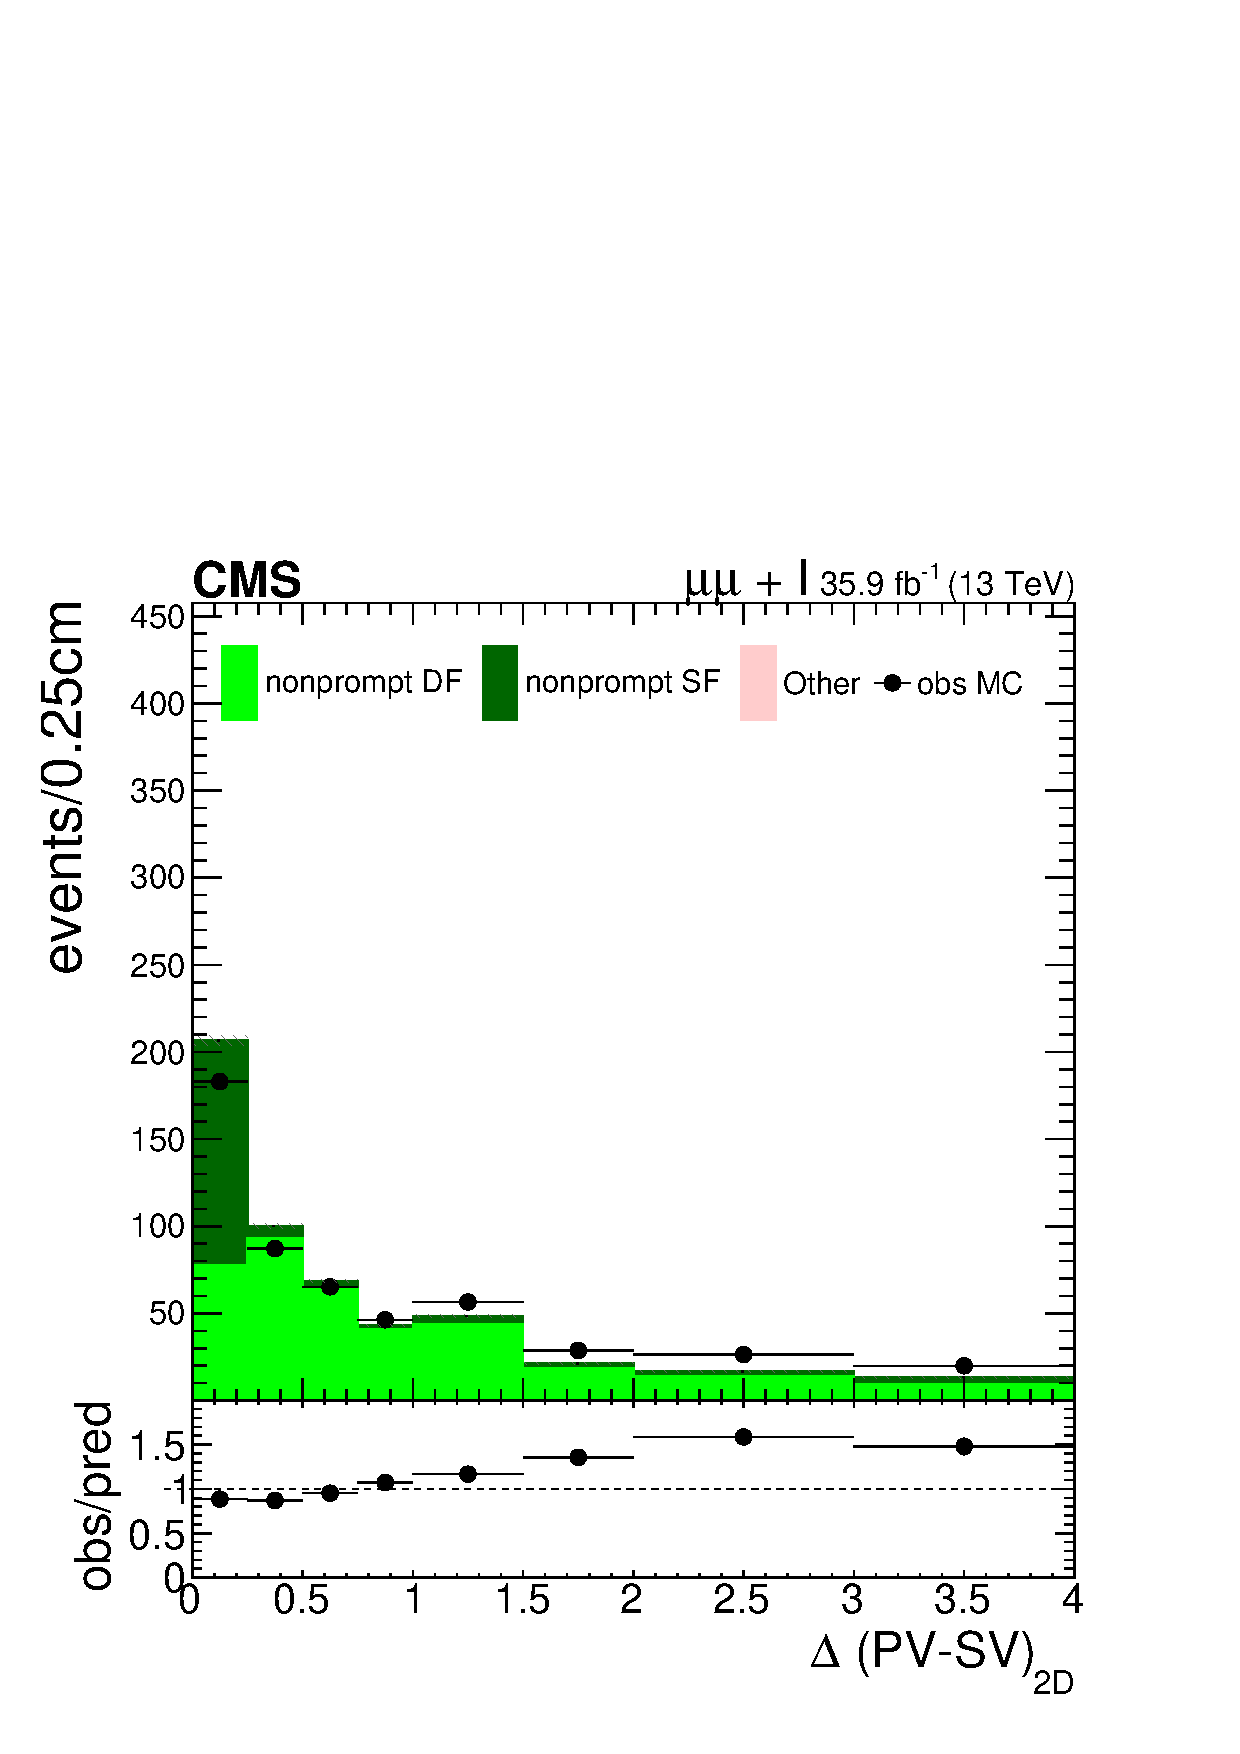
\includegraphics[clip,trim=0.cm 0.cm 0.5cm 0.5cm,height=4.5cm]{Figures/c6/backgrounds/mc_closure/mu_DeltaPV_SV_2D_zomm__0.pdf}
  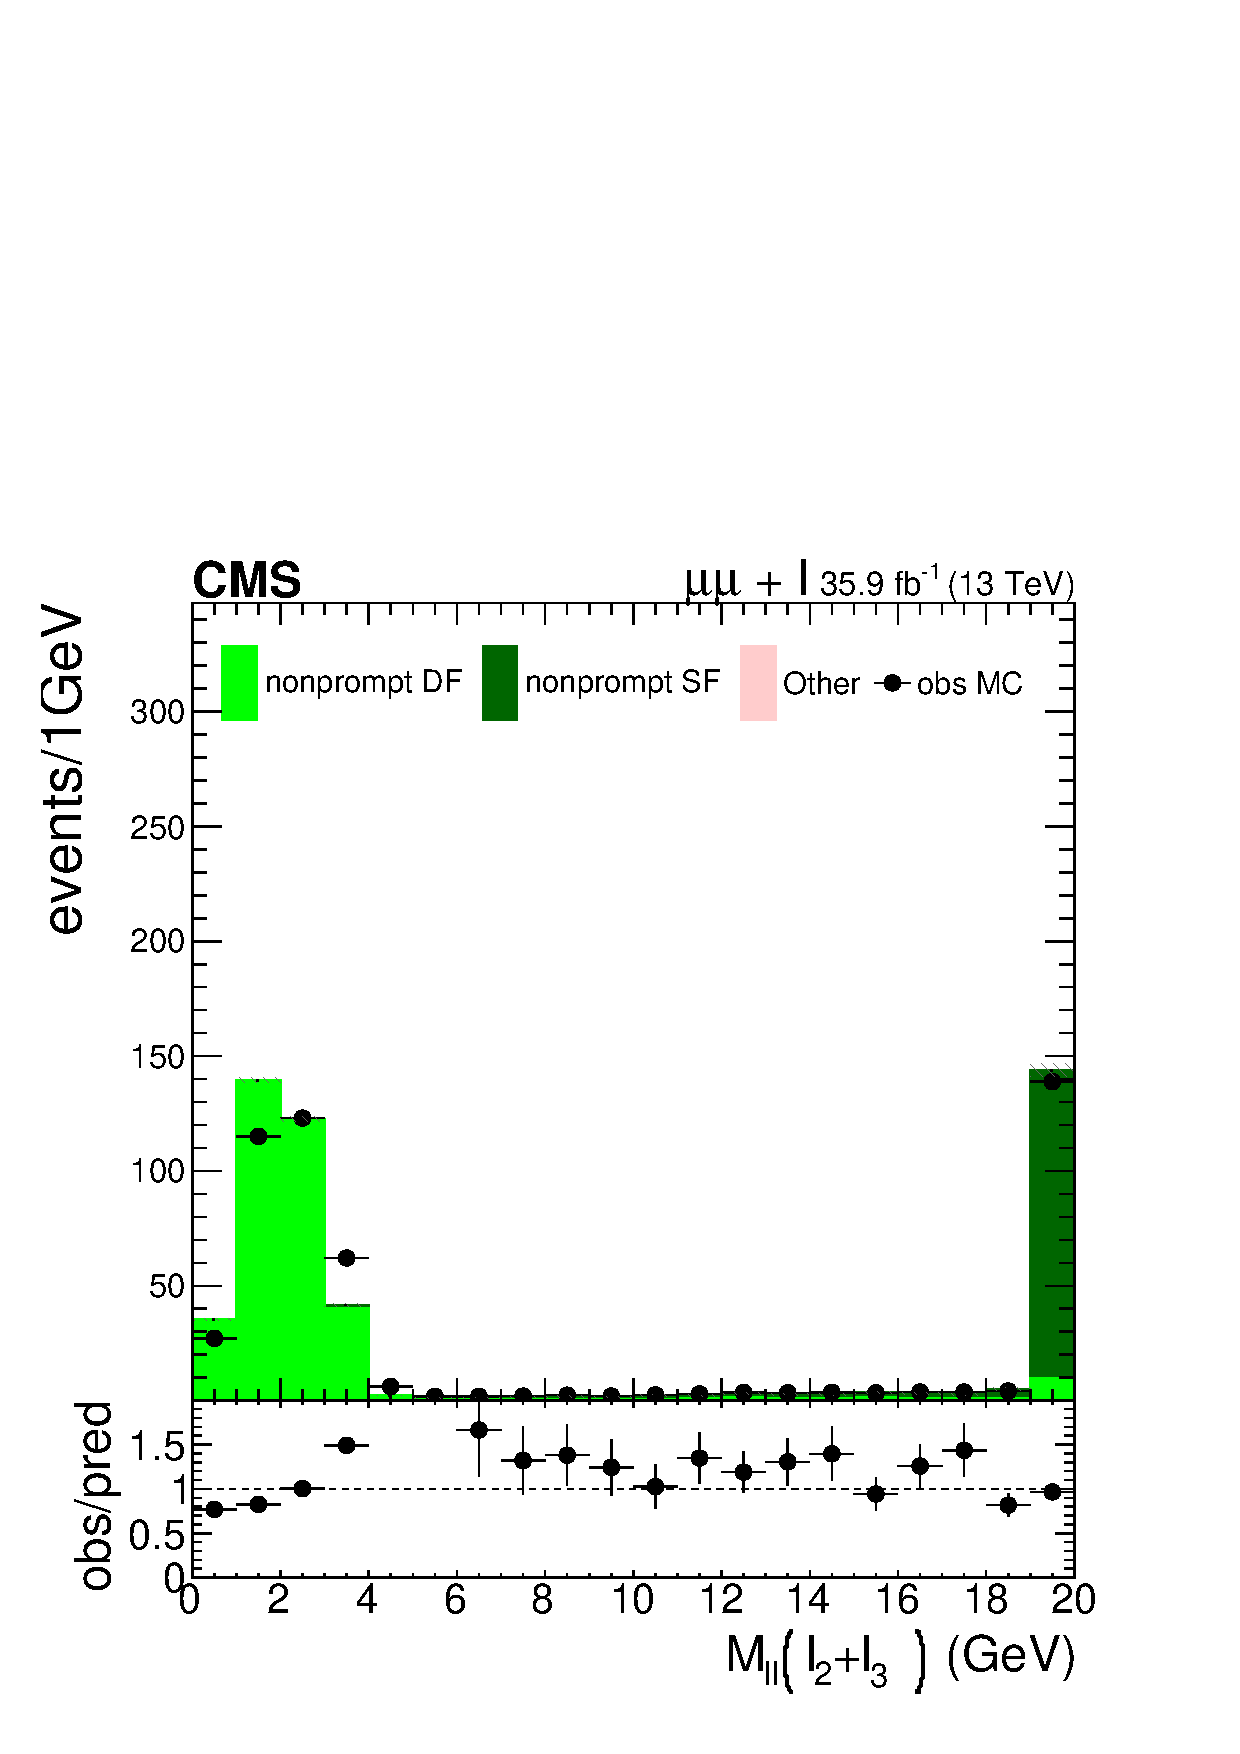
\includegraphics[clip,trim=0.cm 0.cm 0.5cm 0.5cm,height=4.5cm]{Figures/c6/backgrounds/mc_closure/mu_M_ll_l2_l3_zoom__0.pdf}
  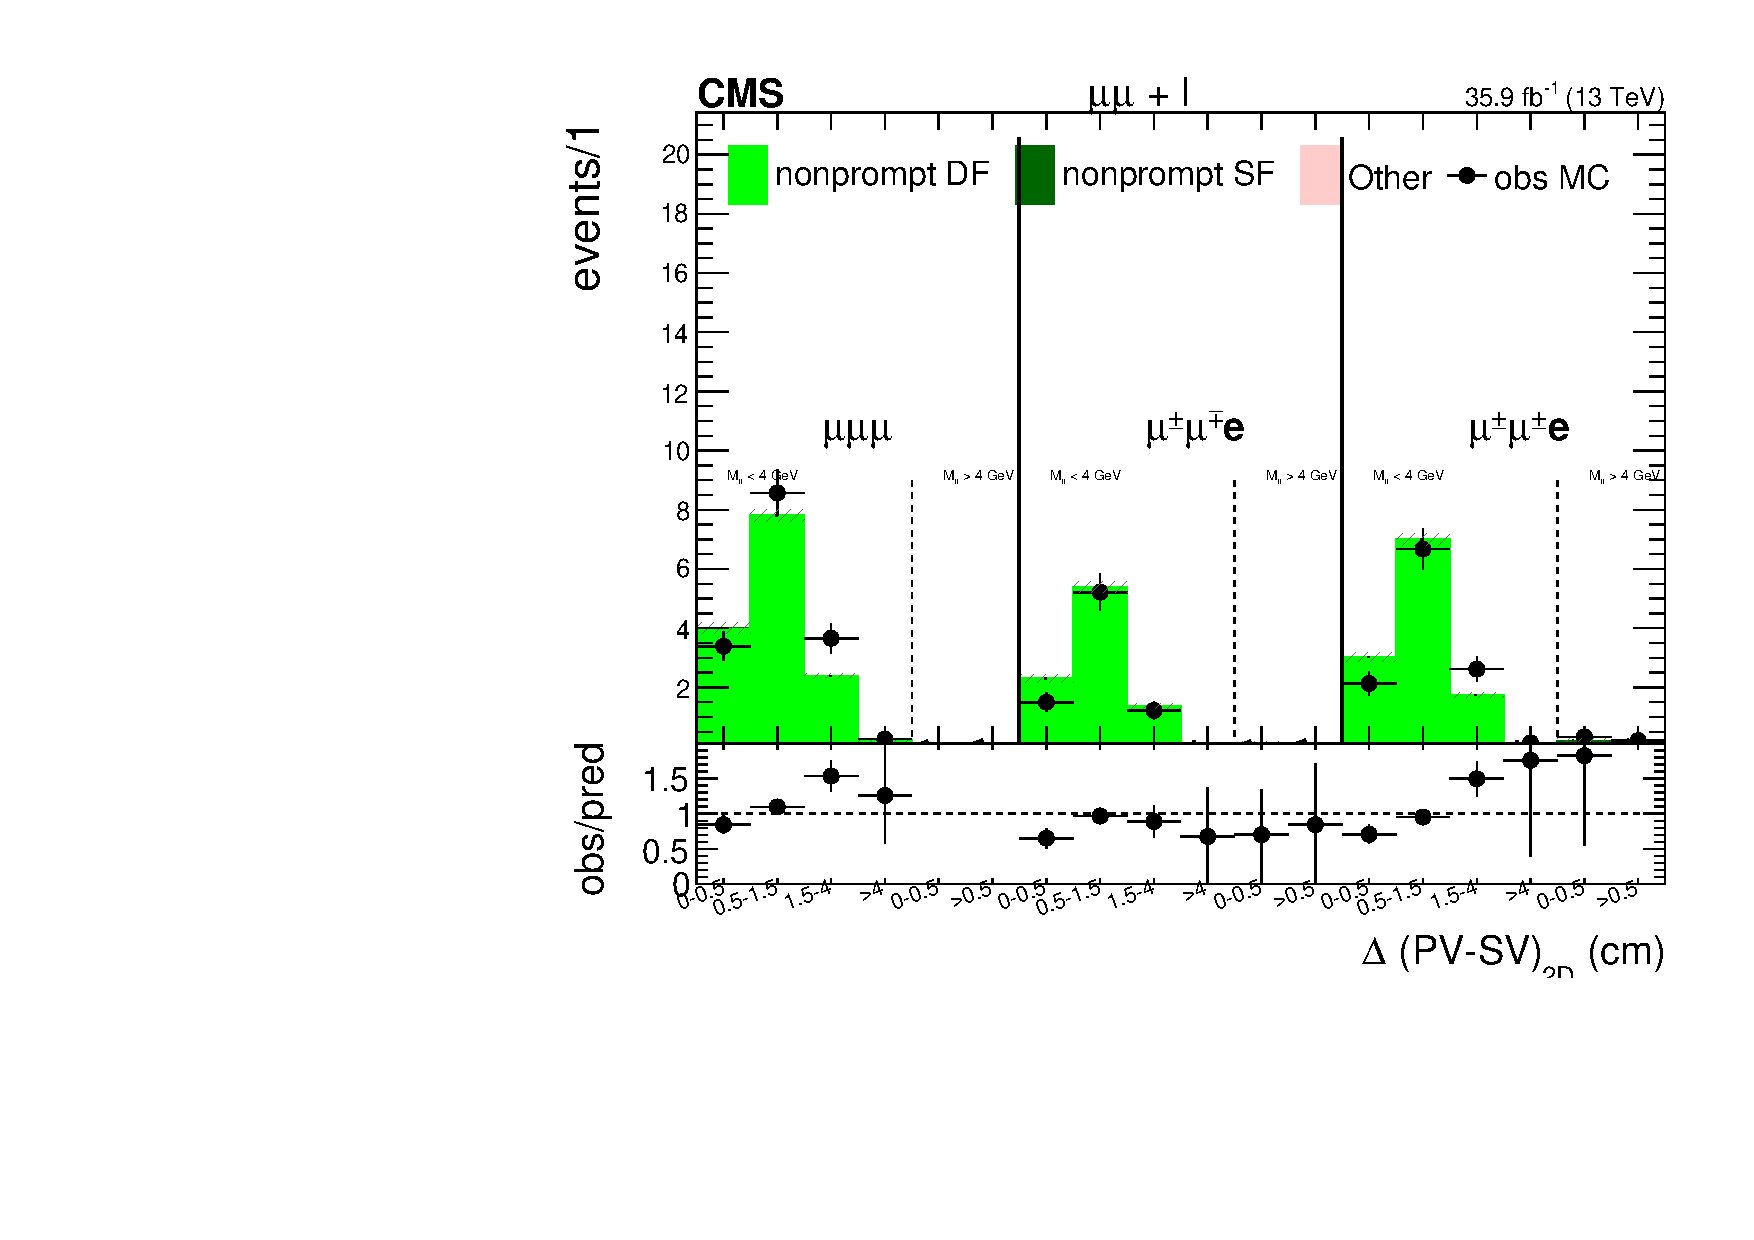
\includegraphics[clip,trim=0.5cm 0.cm 0.5cm 0.5cm,height=4.5cm]{Figures/c6/backgrounds/mc_closure/mu_SR__final.pdf}
  \caption{Distributions of \Deltwod (left), \mtwol (middle)
    2016 \ttbar MC samples,
    comparing the MC events containing SF leptons
    and DF leptons with the
    prediction, for the sum of all final states.
    The right plot shows the signal-region yields after all the event
    selection,~\ref{tab:baselinesel}, has been applied.}
  \label{fig:mcClosure}
\end{figure}

In the following we present data control region orthogonal to the defined search region to test the
prediction power of the method. 


 \paragraph{Closure test in data sample: sideband control region}\label{sec:llsidebandcr}
This control region is defined in Table~\ref{tab:side_band_sel}.
Data in this region are compared to our data-driven (nonprompt DF and
SF) and MC-based (the other) background estimates.

Results for Run2 data are shown in
Figure~\ref{fig:sb_sr_Ctrl}.\\

\begin{table}[h]
  \centering
{\footnotesize
  \caption{\label{tab:side_band_sel} Control region selection requirements
    applied to all data sets.}
    \begin{tabular}{l|l}
    \hline
    Variable     & Requirement       \\
    \hline
    \hline
    \DRtwol      & $<1$              \\
    \minDphi     & $>1$ rad          \\ 
    \mlll     & $< 50$ OR $> 80$\GeV \\
    N. \PQb & $=0$              \\
    (\ltwo $+$ \lthree) \pt & $> 15$ \GeV             \\
    \costheta    & $>0.99$            \\
    \mtwol& $<20$\GeV             \\ 
    $p_{SV} $& $> 0.001$              \\
    $S(\Delta_{2D})$& $>20$              \\ 
    resonance vetoes & \checkmark      \\
    \hline
     \hline
     \mthreel in $\Pe\Pe\Pe$ and $\PGm\PGm\Pe$ OS & $<50$\GeV or $>101$\GeV \\
    \hline
    \hline 
  \end{tabular}
}
\end{table}

\begin{figure}[h]
  \noindent
  \makebox[\textwidth]{
  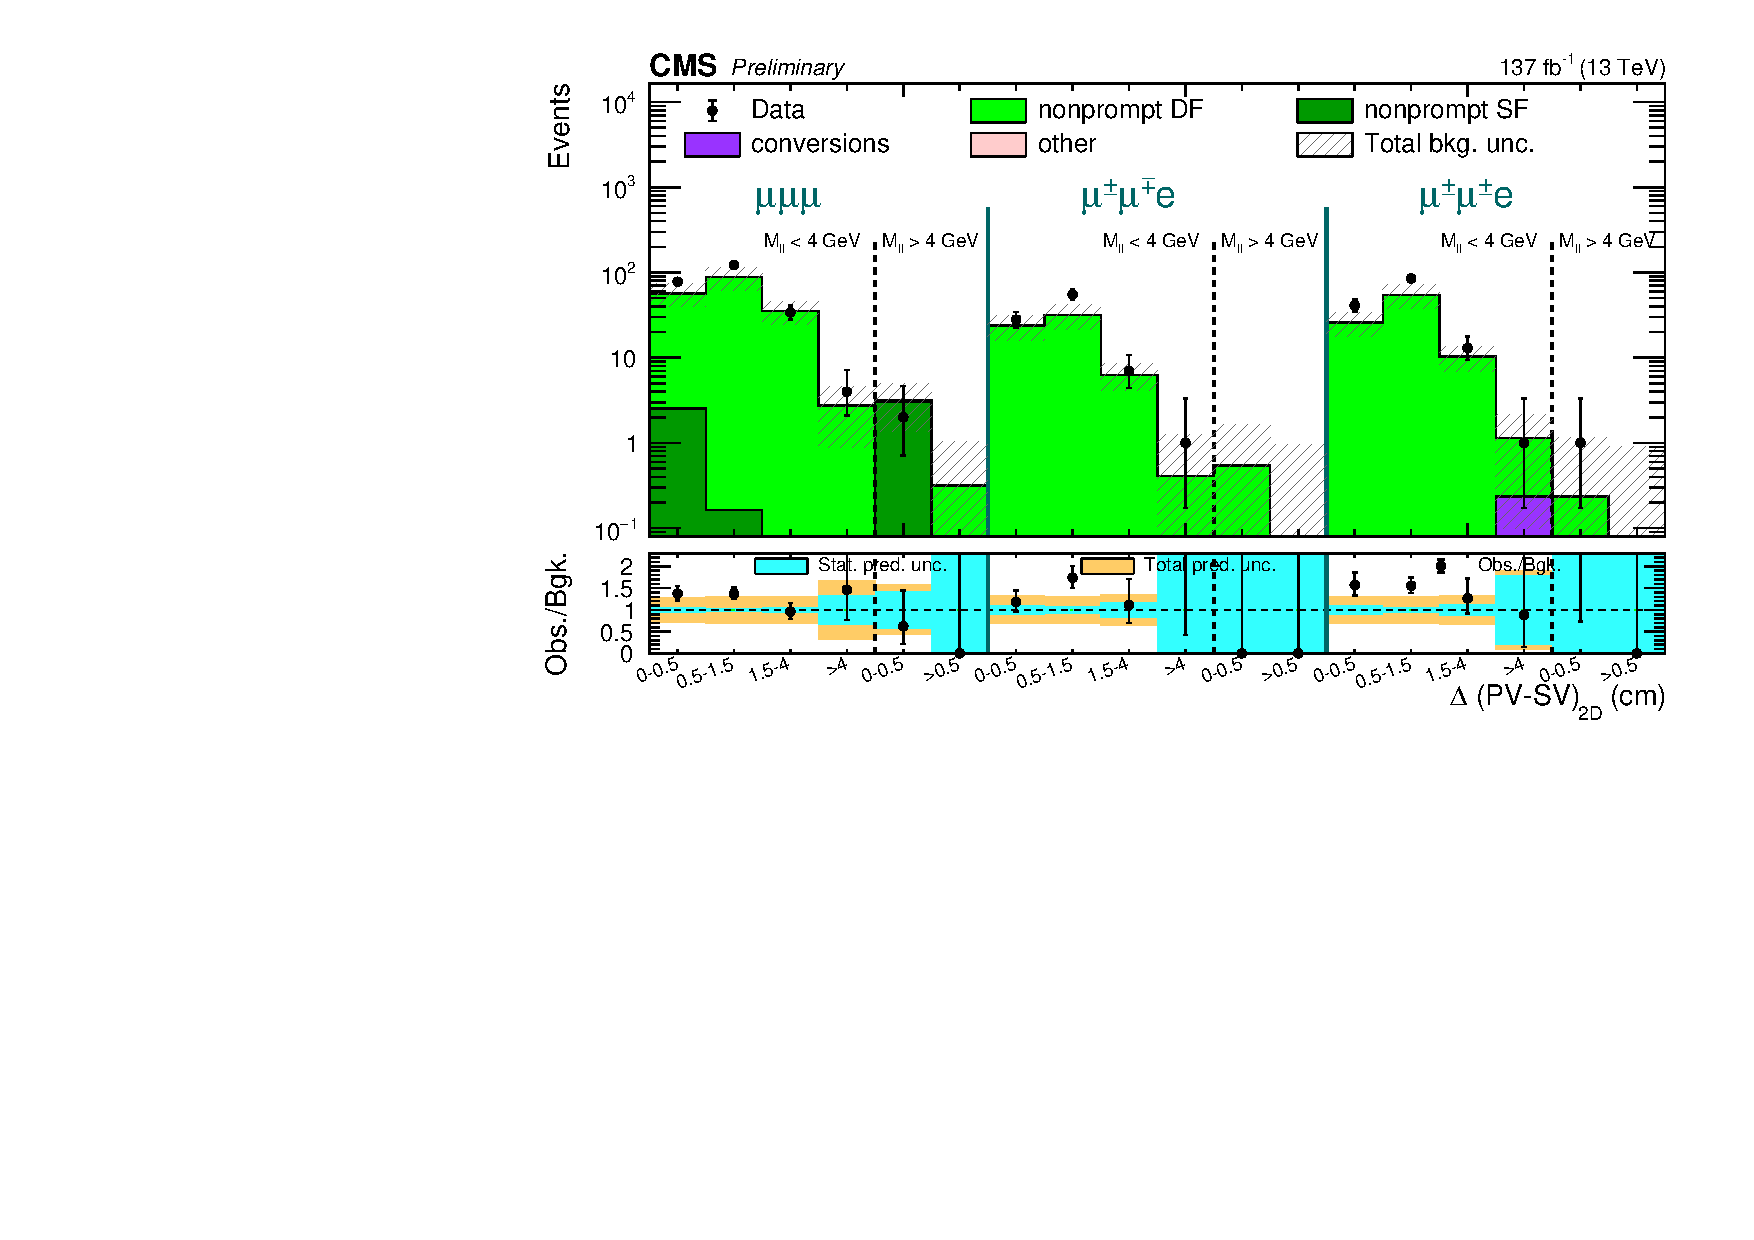
\includegraphics[width=.51\textwidth]{Figures/c6/backgrounds/FR/closureTest/Data/onlySideBand/M-6_V-0p00202484567313_mu_muo_datacard_combined_SR.pdf}
  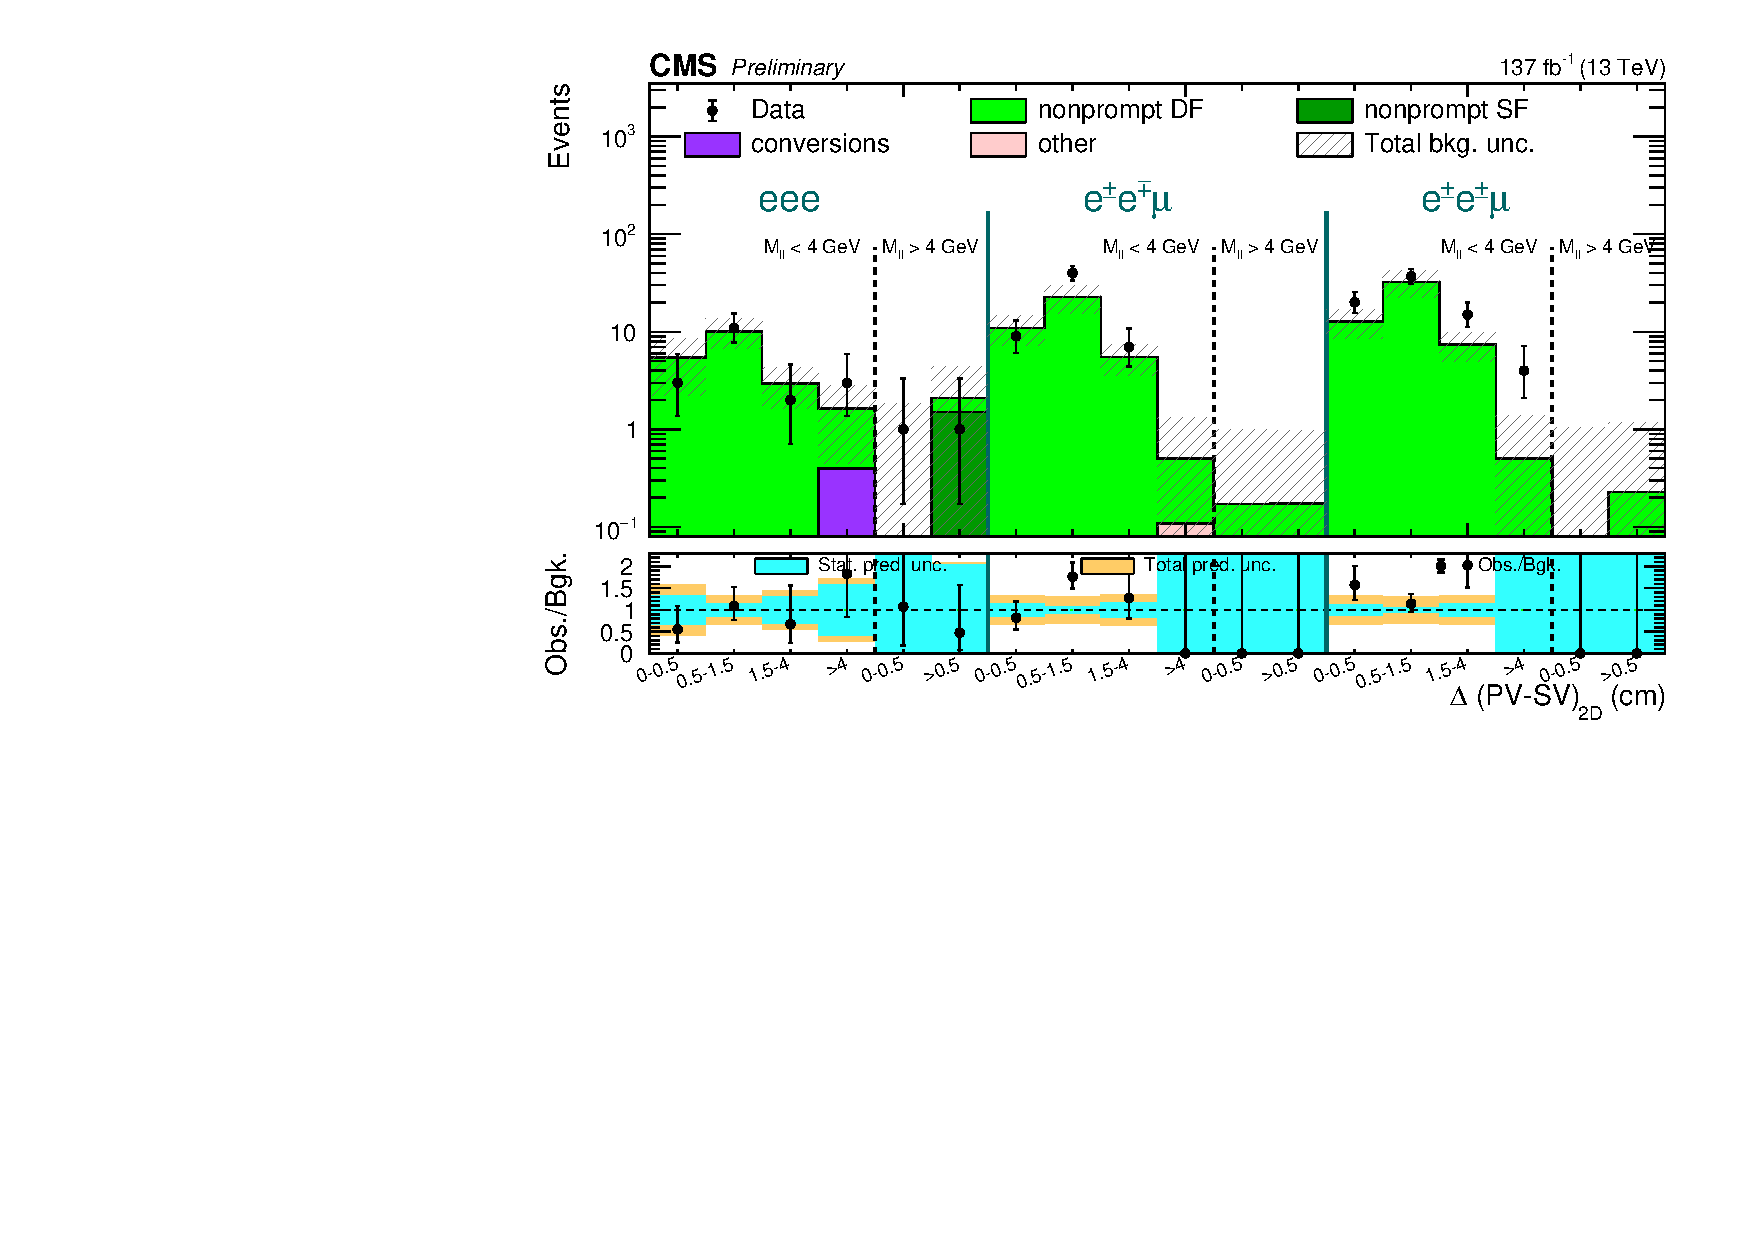
\includegraphics[width=.51\textwidth]{Figures/c6/backgrounds/FR/closureTest/Data/onlySideBand/M-6_V-0p00202484567313_e_ele_datacard_combined_SR.pdf}}\\
\noindent
  \makebox[\textwidth]{
  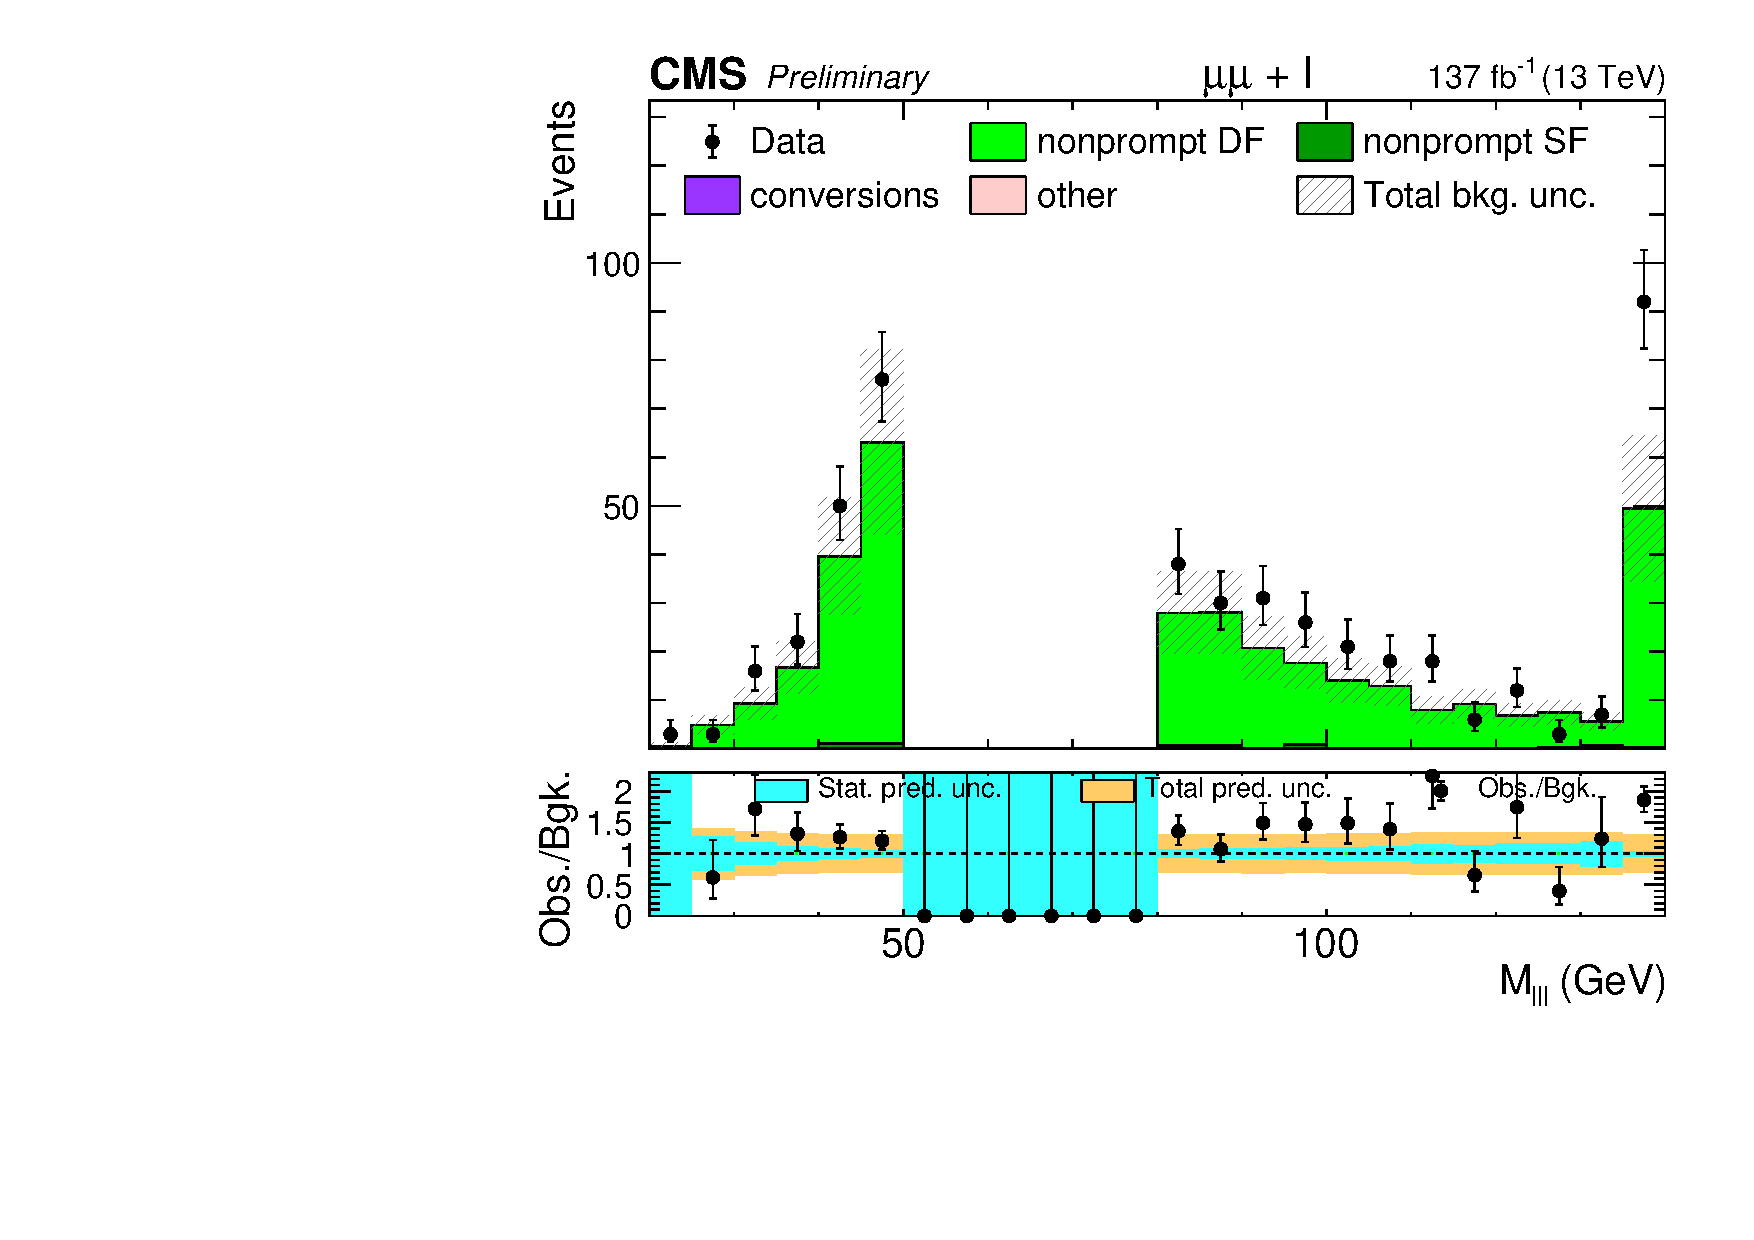
\includegraphics[width=.33\textwidth]{Figures/c6/backgrounds/FR/closureTest/Data/onlySideBand/M-6_V-0p00202484567313_mu_muo_mass3_datacard_combined_mass3.pdf}
  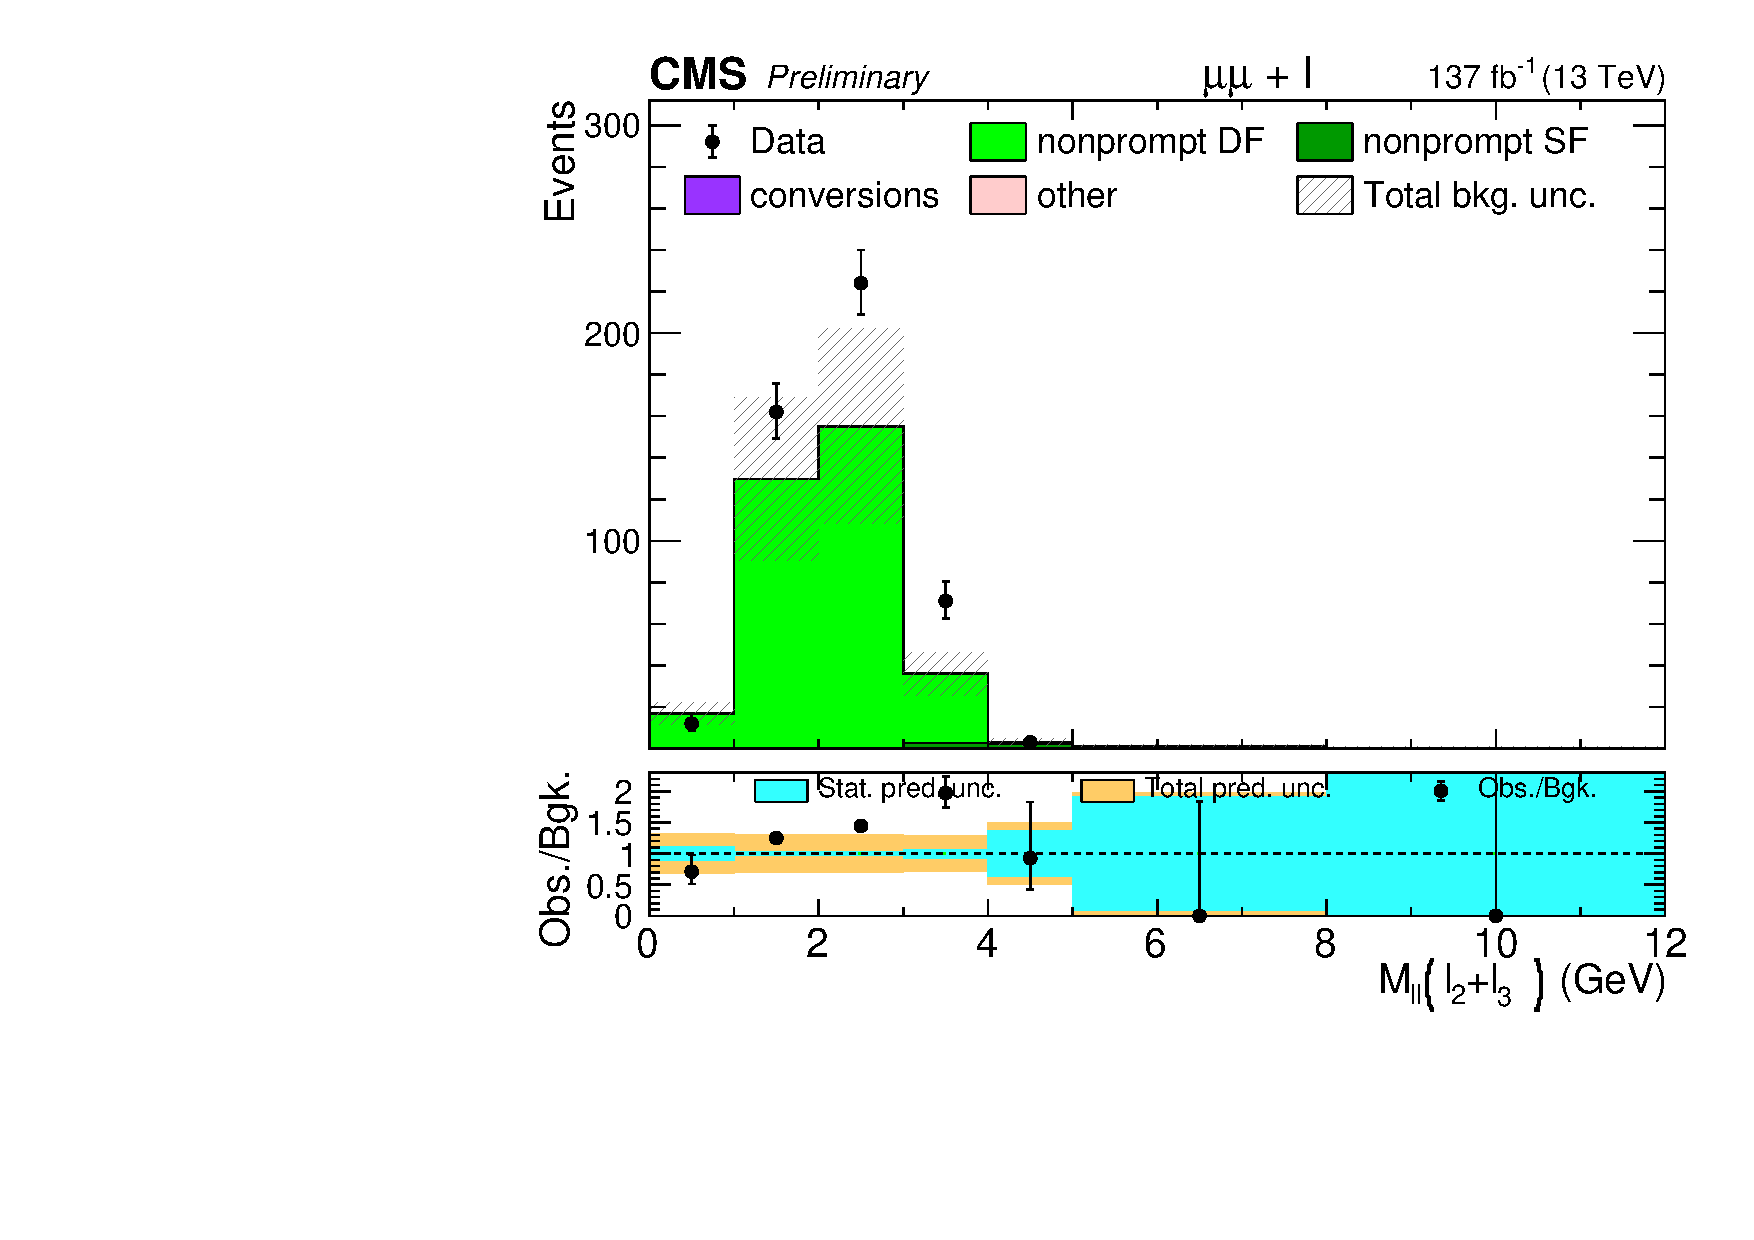
\includegraphics[width=.33\textwidth]{Figures/c6/backgrounds/FR/closureTest/Data/onlySideBand/M-6_V-0p00202484567313_mu_muo_mass_datacard_combined_massl2l3.pdf}
   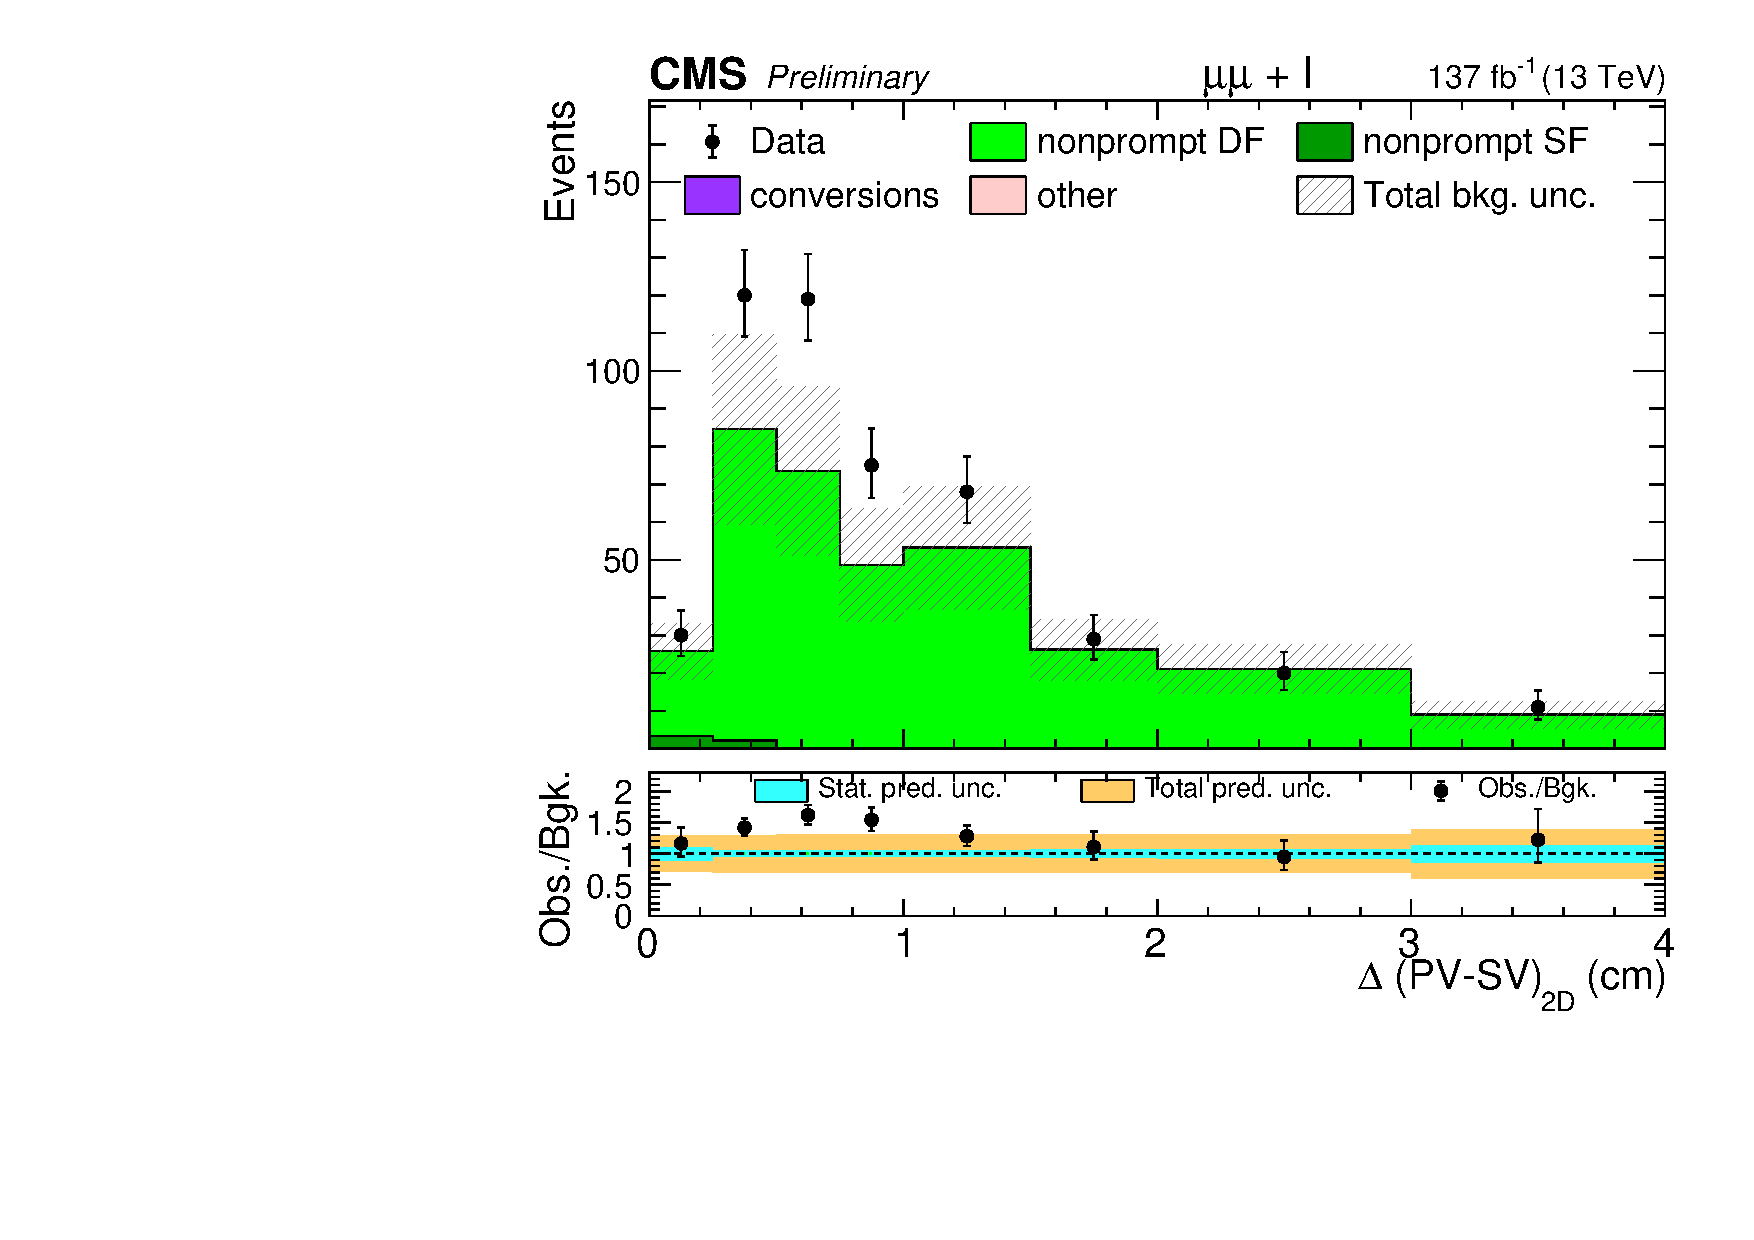
\includegraphics[width=.33\textwidth]{Figures/c6/backgrounds/FR/closureTest/Data/onlySideBand/M-6_V-0p00202484567313_mu_muo_disp_datacard_combined_displacement.pdf}}\\
\noindent
  \makebox[\textwidth]{
  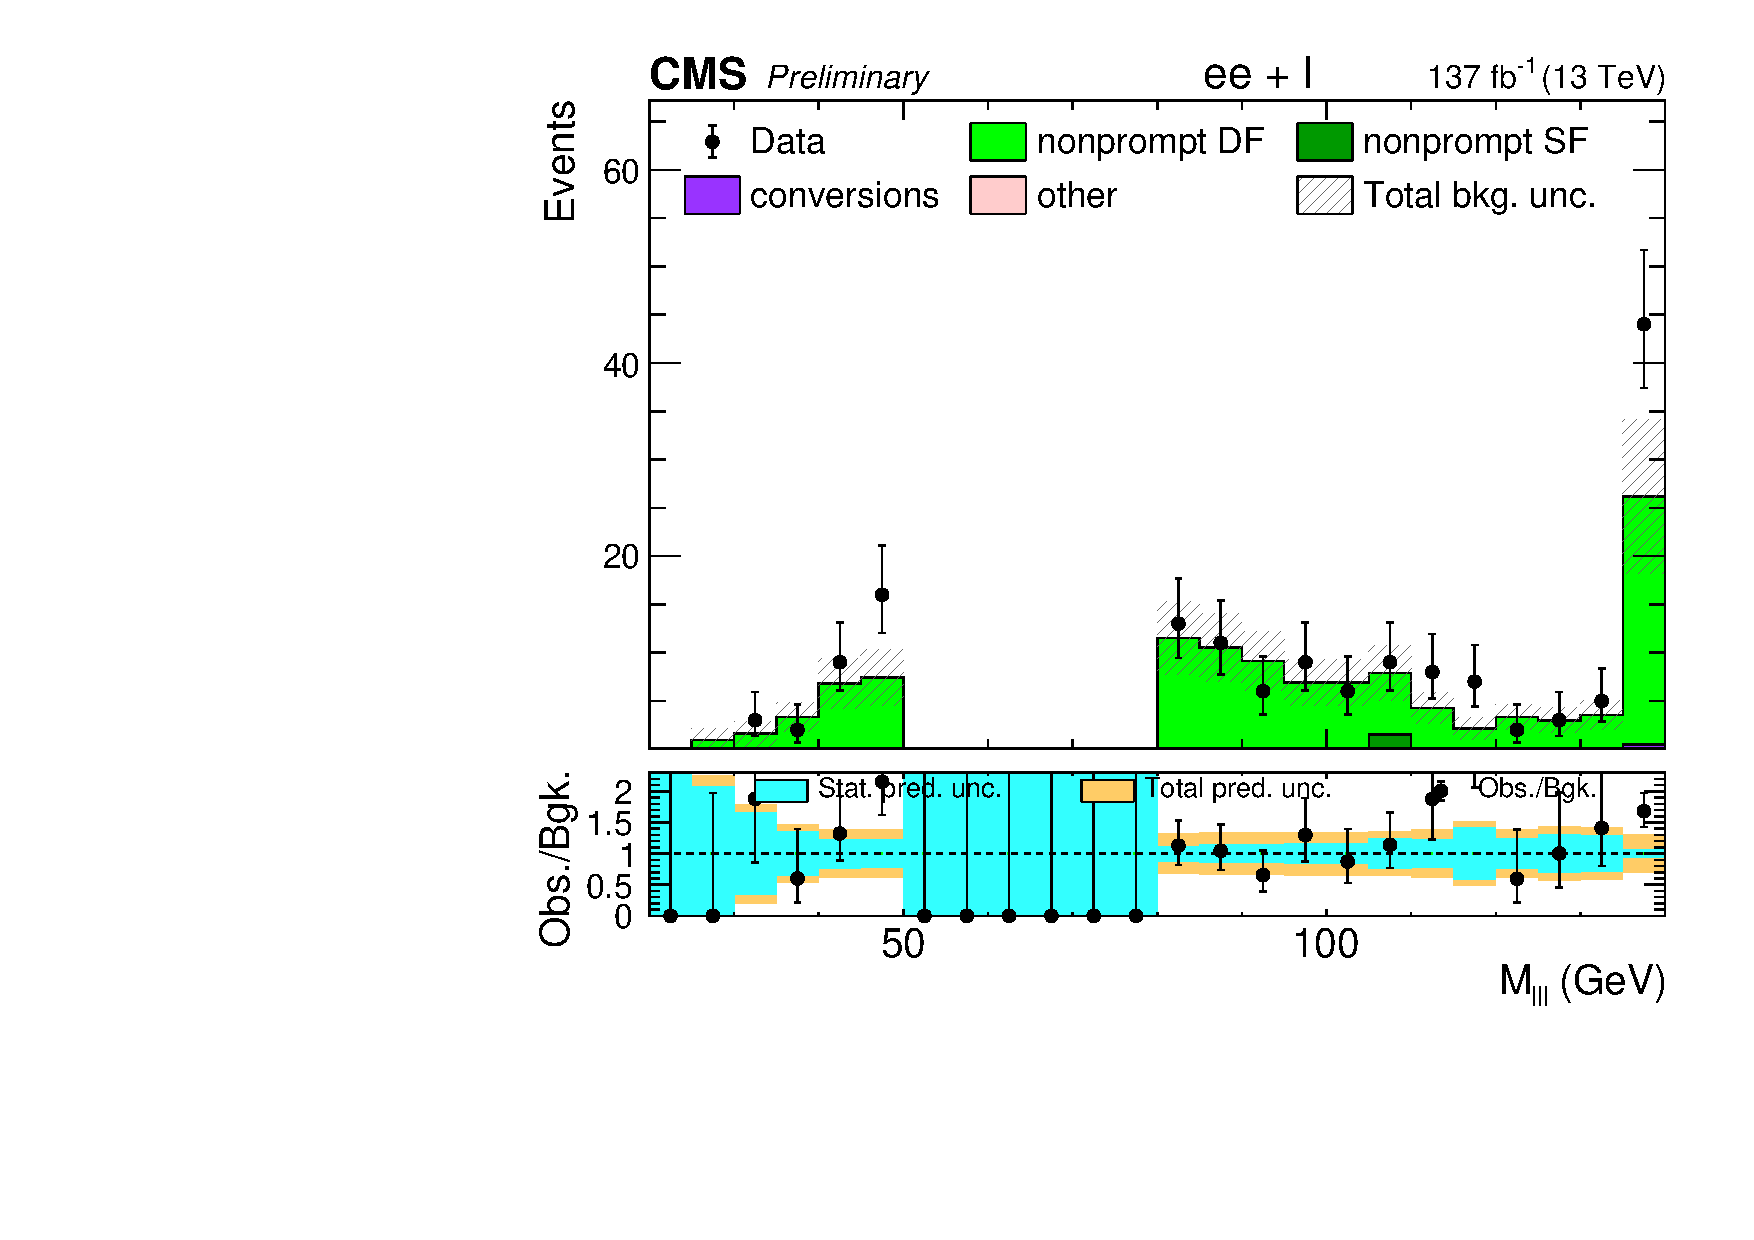
\includegraphics[width=.33\textwidth]{Figures/c6/backgrounds/FR/closureTest/Data/onlySideBand/M-6_V-0p00202484567313_e_ele_mass3_datacard_combined_mass3.pdf}
  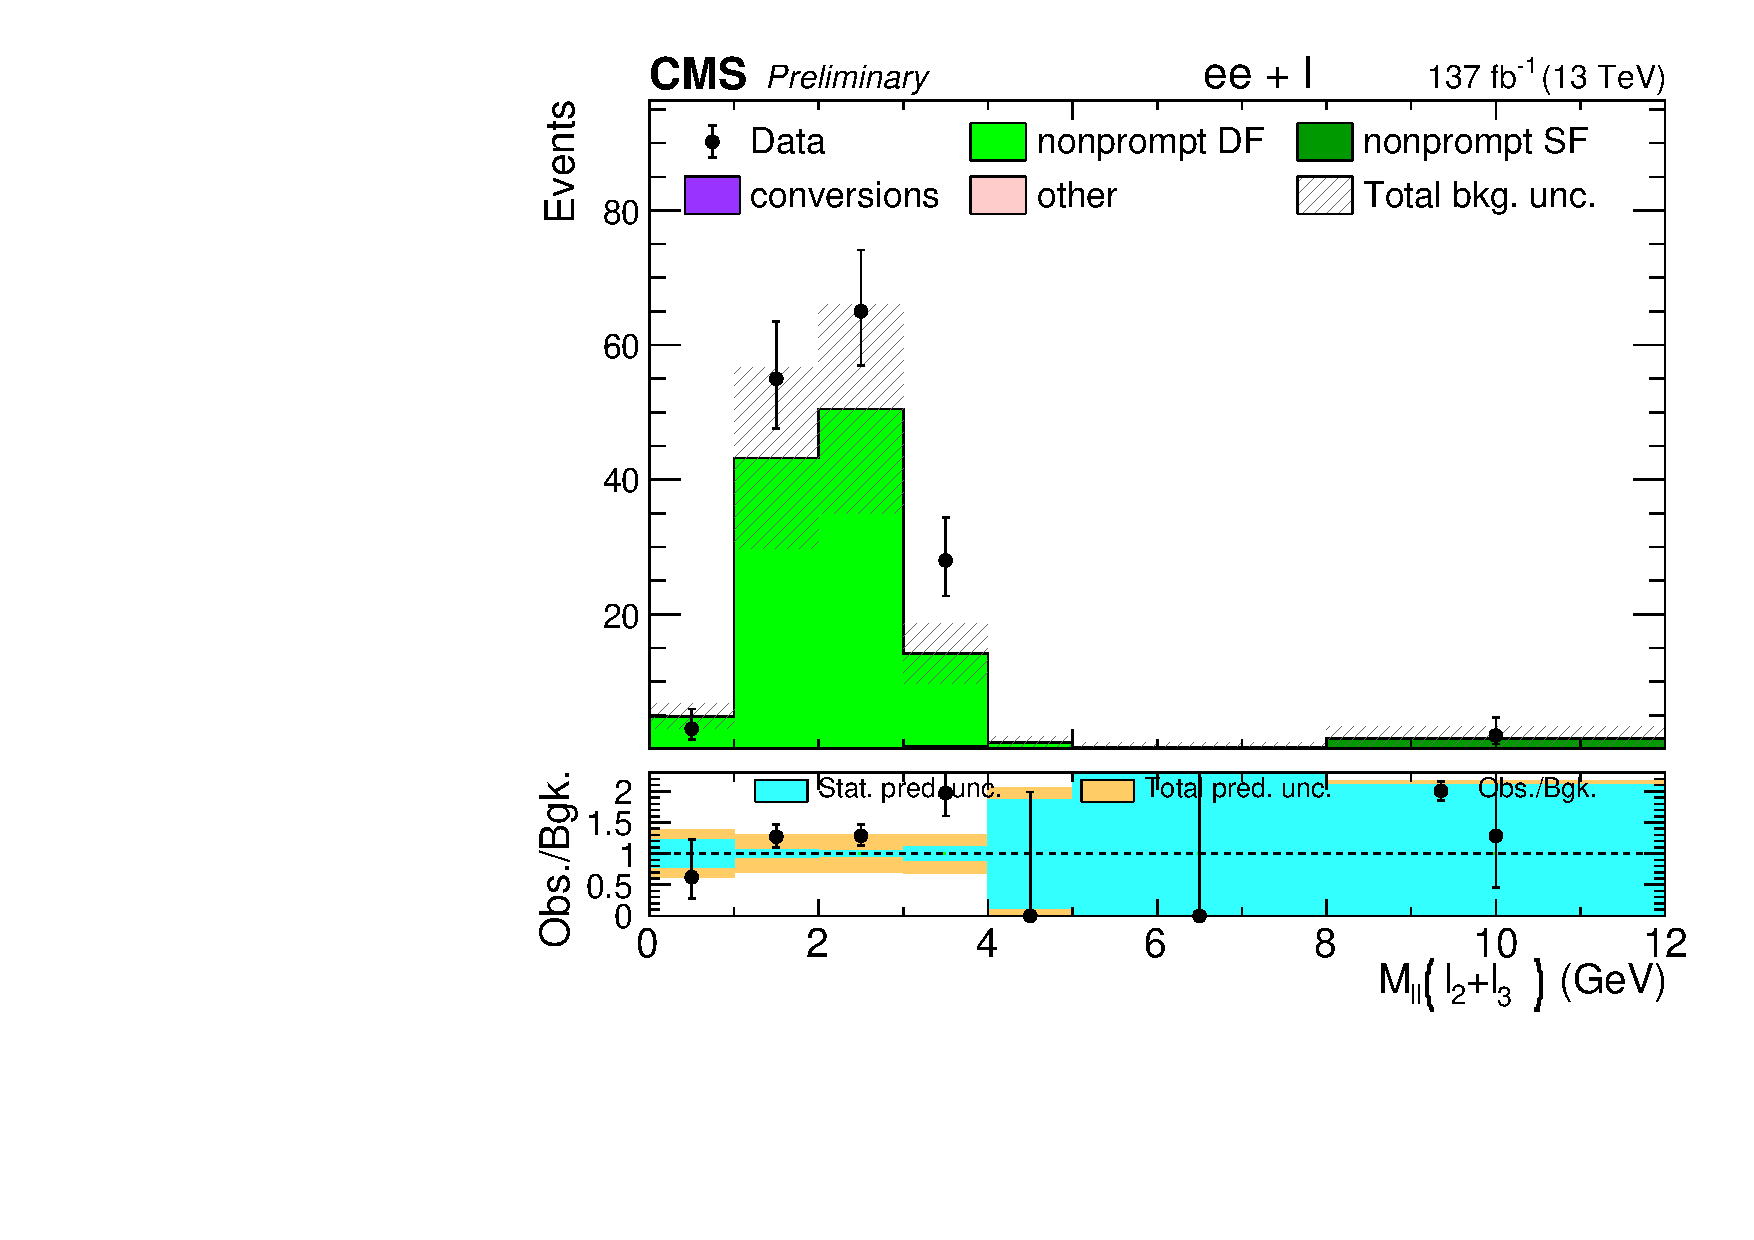
\includegraphics[width=.33\textwidth]{Figures/c6/backgrounds/FR/closureTest/Data/onlySideBand/M-6_V-0p00202484567313_e_ele_mass_datacard_combined_massl2l3.pdf}
   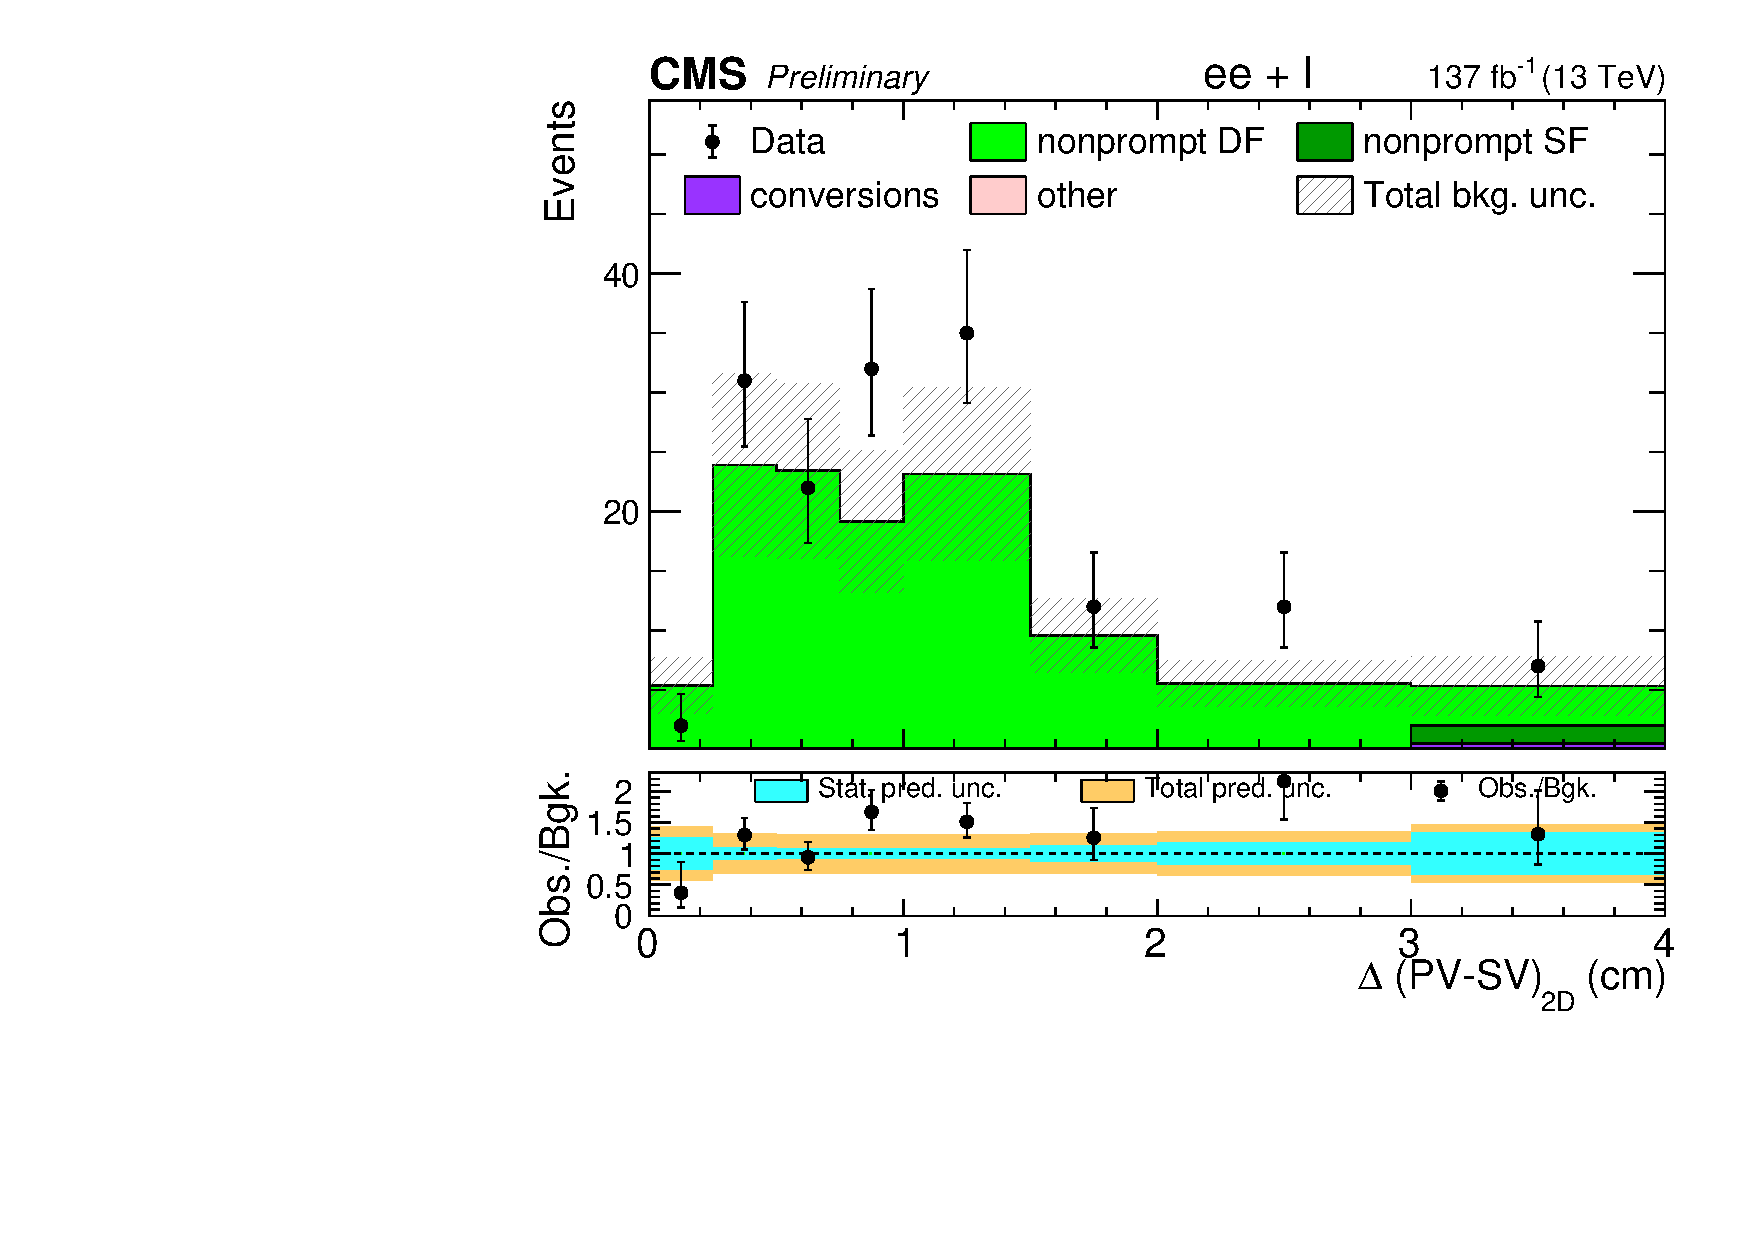
\includegraphics[width=.33\textwidth]{Figures/c6/backgrounds/FR/closureTest/Data/onlySideBand/M-6_V-0p00202484567313_e_ele_disp_datacard_combined_displacement.pdf}}\\
  \caption{At the top, search region-like distributions with the selection of the
    sideband control region, in data and background
    predictions, in final states with more than two muons (left) and
    more than two electrons (right). In the middle and at the bottom, distributions of three-lepton invariant mass (left), \mtwol
    (middle), and \Deltwod (right) in the combined Run2 sideband control region,
    for the sum of all final states with muon couplings (middle) and
    electron couplings (bottom).}
  \label{fig:sb_sr_Ctrl}
\end{figure}
\vspace{10cm}
\paragraph*{Closure test in data sample: \PQb control region}
This control region is defined in Table~\ref{tab:ttbar_sel}.
Data in this region are compared to our data-driven (nonprompt DF and
SF) and MC-based (the other) background estimates.\\
Results for Run2 data are shown in
Figure~\ref{fig:sb_ttbar_Ctrl}.

\begin{table}[h]
  \centering
{\footnotesize
  \caption{\label{tab:ttbar_sel} \PQb control region selection requirements
    applied to all data sets.}
   \begin{tabular}{l|l}
    \hline
    Variable     & Requirement       \\
    \hline
    \hline
    \DRtwol      & $<1$              \\
    \minDphi     & $>1$ rad          \\ 
    %%\mthreel     & $< 50$ OR $> 80\GeV$ \\
    N. \PQb & $\neq 0$              \\
    (\ltwo $+$ \lthree) \pt & $> 15$\GeV              \\
    \costheta    & $>0.99$            \\
    \mtwol& $<20$\GeV              \\ 
    $p_{SV} $& $> 0.001$              \\
    $S(\Delta_{2D})$& $>20$              \\ 
    resonance vetoes & \checkmark      \\
    \hline
     \hline
     \mlll in $\Pe\Pe\Pe$ and $\PGm\PGm\Pe$ OS & $<50$\GeV or $>101$\GeV \\
    \hline
    \hline 
  \end{tabular}
}
\end{table}

\begin{figure}[h]
   \noindent
  \makebox[\textwidth]{
  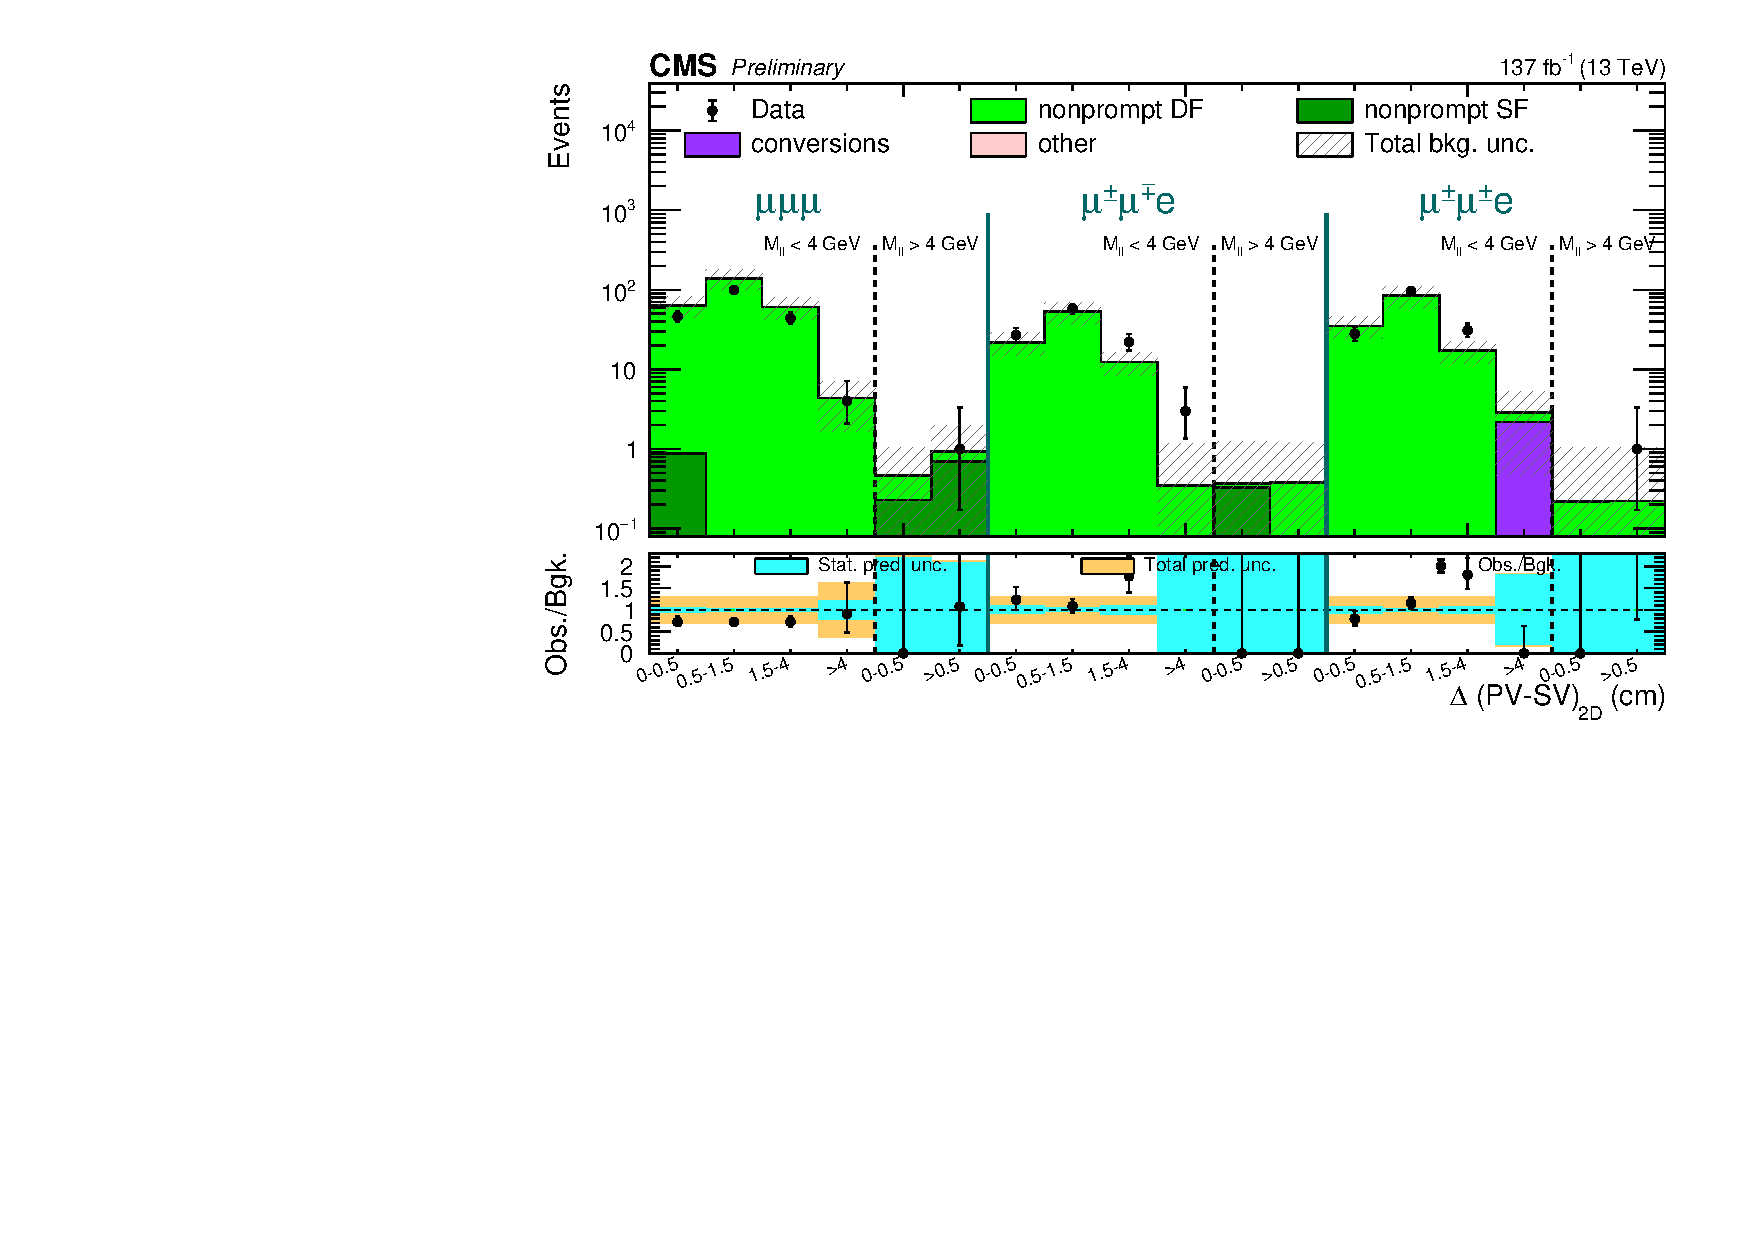
\includegraphics[width=.51\textwidth]{Figures/c6/backgrounds/FR/closureTest/Data/onlyBjet/M-6_V-0p00202484567313_mu_muo_datacard_combined_SR.pdf}
  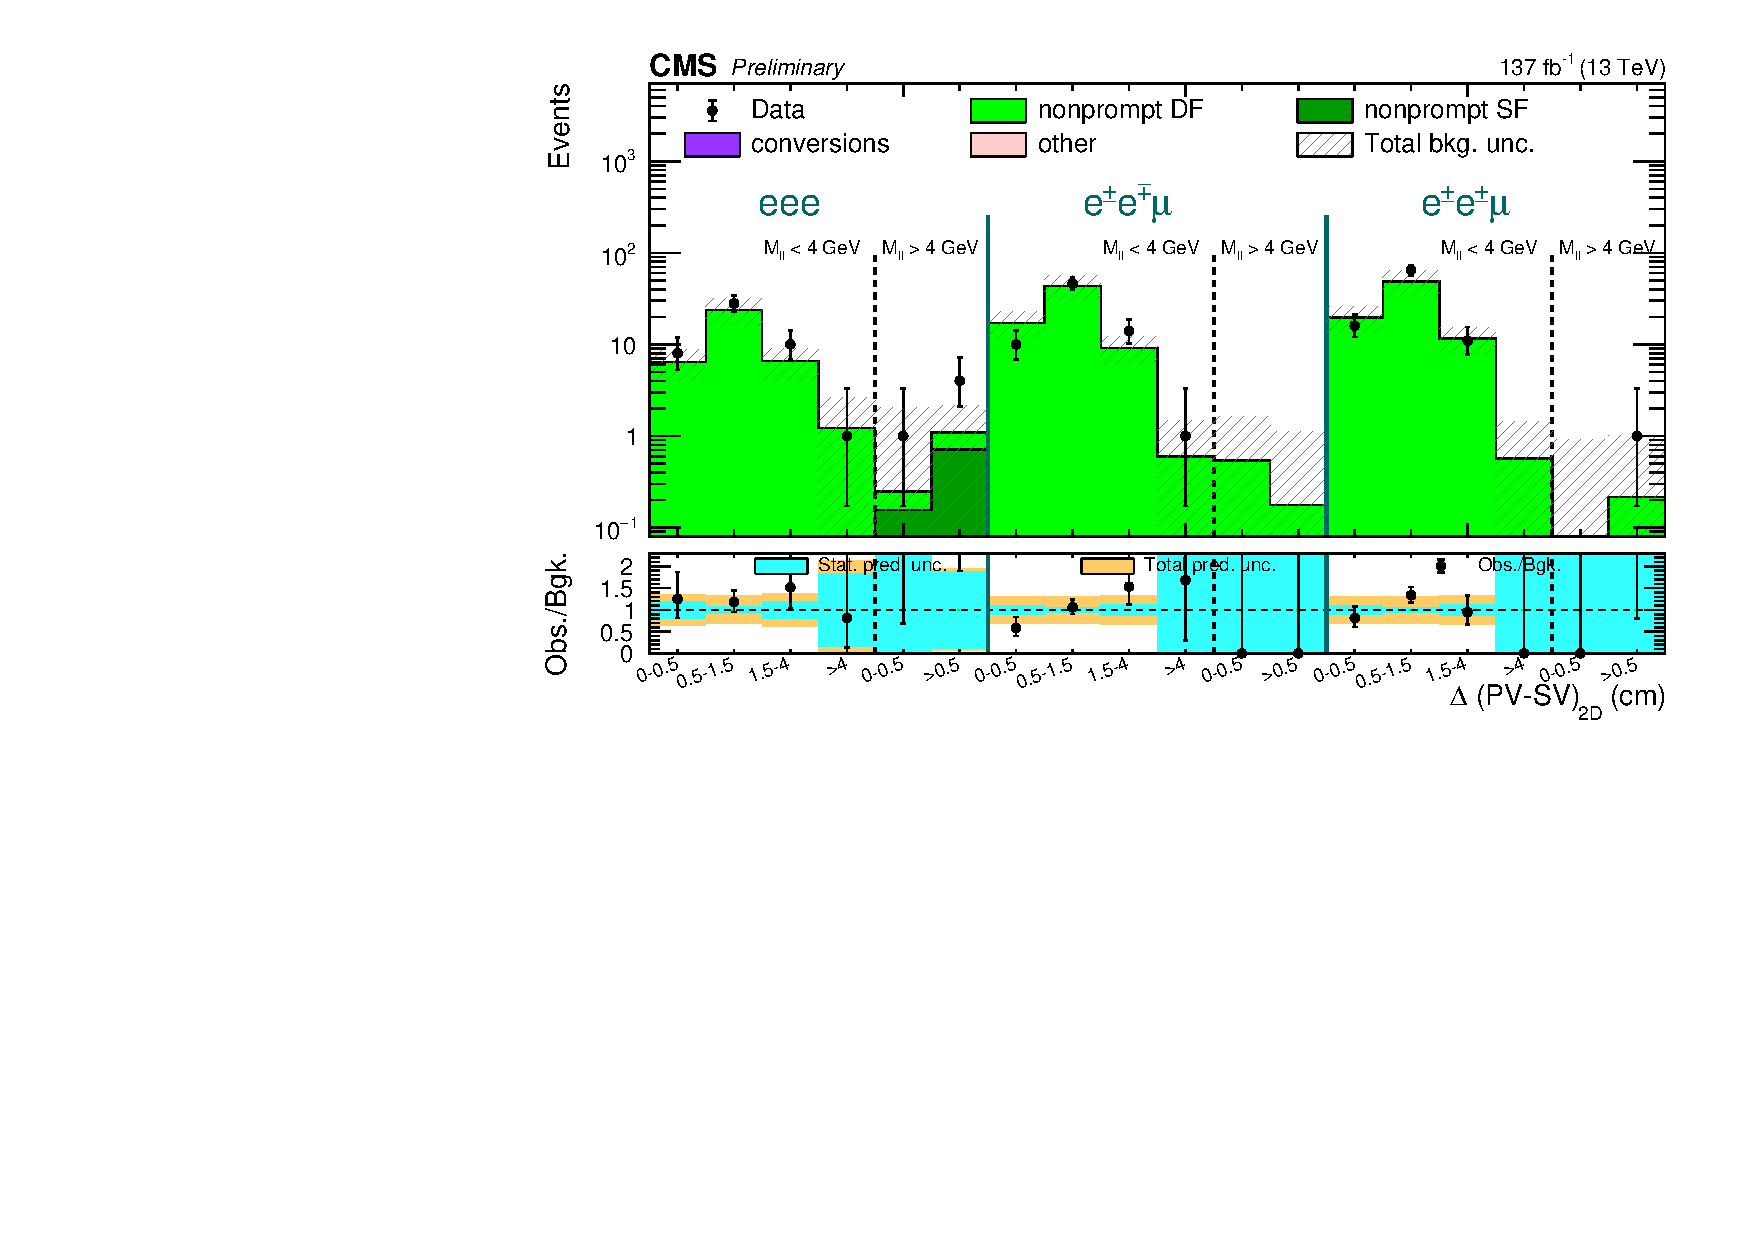
\includegraphics[width=.51\textwidth]{Figures/c6/backgrounds/FR/closureTest/Data/onlyBjet/M-6_V-0p00202484567313_e_ele_datacard_combined_SR.pdf}}\\
\noindent
  \makebox[\textwidth]{
  \includegraphics[width=.33\textwidth]{Figures/c6/backgrounds/FR/closureTest/Data/onlyBjet/M-6_V-0p00202484567313_mu_muo_mass3_datacard_combined_mass3.pdf}
  \includegraphics[width=.33\textwidth]{Figures/c6/backgrounds/FR/closureTest/Data/onlyBjet/M-6_V-0p00202484567313_mu_muo_mass_datacard_combined_massl2l3.pdf}
   \includegraphics[width=.33\textwidth]{Figures/c6/backgrounds/FR/closureTest/Data/onlyBjet/M-6_V-0p00202484567313_mu_muo_disp_datacard_combined_displacement.pdf}}\\
\noindent
  \makebox[\textwidth]{
  \includegraphics[width=.33\textwidth]{Figures/c6/backgrounds/FR/closureTest/Data/onlyBjet/M-6_V-0p00202484567313_e_ele_mass3_datacard_combined_mass3.pdf}
  \includegraphics[width=.33\textwidth]{Figures/c6/backgrounds/FR/closureTest/Data/onlyBjet/M-6_V-0p00202484567313_e_ele_mass_datacard_combined_massl2l3.pdf}
   \includegraphics[width=.33\textwidth]{Figures/c6/backgrounds/FR/closureTest/Data/onlyBjet/M-6_V-0p00202484567313_e_ele_disp_datacard_combined_displacement.pdf}}\\
  \caption{Search region-like distributions with the selection of the
    \PQb control region, in data and background
    predictions, in final states with more than two muons (left) and
    more than two electrons (right). In the middle and at the bottom, distributions of three-lepton invariant mass (left), \mtwol
    (middle), and \Deltwod (right) in the combined Run2 sideband control region,
    for the sum of all final states with muon couplings (middle) and
    electron couplings (bottom).}
  \label{fig:sb_ttbar_Ctrl}
\end{figure}


\paragraph{Closure test in data sample: sideband plus b jet control region}
Taking into account the complementary of the two control regions just
presented above and considering the low statistic of the
Figure~\ref{fig:sb_sr_Ctrl}, a new CR has been defined. \\
Results for Run2 data  are shown in
Figure~\ref{fig:CR_dist}.
\begin{table}[h!]
  \centering
{\footnotesize
  \caption{\label{tab:sideband_plus_bjet_table} Control region selection requirements
    applied to all data sets.}
    \begin{tabular}{l|l}
    \hline
    Variable     & Requirement       \\
    \hline
    \hline
    \DRtwol      & $<1$              \\
    \minDphi     & $>1$ rad          \\ 
    (\ltwo $+$ \lthree) \pt & $> 15$\GeV          \\
    \costheta    & $>0.99$            \\
    \mtwol& $<20$\GeV              \\ 
    $p_{SV} $& $> 0.001$              \\
    $S(\Delta_{2D})$& $>20$              \\ 
    resonance vetoes & \checkmark      \\
    \hline
    \multirow{2}{*}{\mthreel  and  N. \PQb } & ($<50$\GeV or
                                                   $>80$\GeV and
                                                   N.\PQb = 0) \\
      & OR
                                                   (N.\PQb $\neq$
                                                   0)\\
     \hline
     \mthreel in $\Pe\Pe\Pe$ and $\PGm\PGm\Pe$ OS & $<50$\GeV or $>101$\GeV \\
    \hline
    \hline 
  \end{tabular}
}
\end{table}
     

This control region combines the b jet and the sideband control
regions and it is defined by the criteria listed in Table~\ref{tab:sideband_plus_bjet_table}. It is obvious that the combination of these two regions 
is done in a fully orthogonal region with respect to the signal region. \\
  
\begin{figure}[h]
  \noindent
  \makebox[\textwidth]{
  \includegraphics[width=.51\textwidth]{Figures/c6/backgrounds/FR/closureTest/Data/SideBandPlusBjet/mu_cr.pdf}
  \includegraphics[width=.51\textwidth]{Figures/c6/backgrounds/FR/closureTest/Data/SideBandPlusBjet/ele_cr.pdf}}\\
\noindent
  \makebox[\textwidth]{
  \includegraphics[width=.33\textwidth]{Figures/c6/backgrounds/FR/closureTest/Data/SideBandPlusBjet/M-6_V-0p00202484567313_mu_muo_mass3_datacard_combined_mass3.pdf}
  \includegraphics[width=.33\textwidth]{Figures/c6/backgrounds/FR/closureTest/Data/SideBandPlusBjet/M-6_V-0p00202484567313_mu_muo_mass_datacard_combined_massl2l3.pdf}
   \includegraphics[width=.33\textwidth]{Figures/c6/backgrounds/FR/closureTest/Data/SideBandPlusBjet/M-6_V-0p00202484567313_mu_muo_disp_datacard_combined_displacement.pdf}}\\
\noindent
  \makebox[\textwidth]{
  \includegraphics[width=.33\textwidth]{Figures/c6/backgrounds/FR/closureTest/Data/SideBandPlusBjet/M-6_V-0p00202484567313_e_ele_mass3_datacard_combined_mass3.pdf}
  \includegraphics[width=.33\textwidth]{Figures/c6/backgrounds/FR/closureTest/Data/SideBandPlusBjet/M-6_V-0p00202484567313_e_ele_mass_datacard_combined_massl2l3.pdf}
   \includegraphics[width=.33\textwidth]{Figures/c6/backgrounds/FR/closureTest/Data/SideBandPlusBjet/M-6_V-0p00202484567313_e_ele_disp_datacard_combined_displacement.pdf}}\\
 \caption{Distributions of three-lepton invariant mass (left), \mtwol
    (middle), and \Deltwod (right) in the combined Run2 control region in table~\ref{tab:sideband_plus_bjet_table},
    for the sum of all final states with muon couplings (top) and
    electron couplings (bottom).}
  \label{fig:CR_dist}
\end{figure}



\vspace{10cm}
\paragraph{Closure test in data sample: validation of internal and external conversions }
\label{sec:conversion}
The photon conversion background is modeled using simulated events,
 but its overall normalization is checked in a
 $\PZ\to\ell^-\ell^+\PGg^{(\ast)}$
 control region in data, as defined in Table~\ref{tab:conv_sel}.
 \begin{table}[h!]
  \centering
{\footnotesize
  \caption{\label{tab:conv_sel} Conversion control region selection requirements
    applied to all data sets.}
    \begin{tabular}{l|l}
    \hline
    Variable     & Requirement       \\
    \hline
    \hline
    \DRtwol      & $<1$              \\
    \minDphi     & $>1$ rad          \\
    \mthreel     & between 81 and 101\GeV, \ie consistent with an on-shell \PZ boson \\
    N. \PQb & $=0$              \\
    (\ltwo $+$ \lthree) \pt & $> 15$\GeV         \\
    \costheta    & $>0.99$            \\
    \mtwol& $<20$\GeV              \\ 
    $p_{SV} $& $> 0.001$              \\
    $S(\Delta_{2D})$& $>20$              \\  
    resonance vetoes &  \checkmark      \\
    \hline
    \hline
  \end{tabular}
}
\end{table}

 This region is dominated by $\PZ\to\ell^-\ell^+\PGg\to\ell^-\ell^+\Pe$
 events, with an asymmetric conversion of the real photon.
 The \mthreel and \mtwol spectra of such events are shown in
 Figures~\ref{fig:phoConv}. A fair agreement is found between data and
 simulation, with no
 corrections required.
 
 \begin{figure}[h]
\centering
\includegraphics[height=3.5cm]{Figures/c6/backgrounds/FR/closureTest/Data/conversion/M-6_V-0p00202484567313_e_ele_datacard_combined_SR.pdf}
  \includegraphics[height=3.5cm]{Figures/c6/backgrounds/FR/closureTest/Data/conversion/M-6_V-0p00202484567313_e_ele_mass_datacard_combined_massl2l3.pdf}
  \includegraphics[height=3.5cm]{Figures/c6/backgrounds/FR/closureTest/Data/conversion/M-6_V-0p00202484567313_e_ele_disp_datacard_combined_displacement.pdf}
    \caption{Distribution of SR-like bins, the two-lepton invariant
    masses, \mtwol, and \Deltwod in the photon-conversion control
    region with events with at least 2 electrons in the final state. Run2.}
  \label{fig:phoConv}
\end{figure}

\clearpage
\section{Signal efficiency validation}\label{sec:llcorrection_efficiencies}

\subsection{Prompt lepton efficiency} \label{sec:promptleptoneff}
Prompt electron and muon identification and isolation efficiencies
are measured in data and simulation using a tag-and-probe method,
applied to samples of inclusive Z boson events.
The data-to-MC ratios of efficiencies (``scale factors'')
measured centrally by the \emph{muon physics object group} as a
function of the lepton \pt and \sigeta are
used to correct the simulated events. Additionally, the scale factors
are measured for the isolation requirement and the impact
parameter cuts. The results are presented in
Figure~\ref{fig:isoip_muon_prompt}.
\begin{figure}[h]
\centering
  \includegraphics[width=.45\textwidth]{Figures/c6/efficiencies/muons/2018/isoip_prompt_sf_2018.pdf}
  \includegraphics[width=.45\textwidth]{Figures/c6/efficiencies/muons/2018/isoip_prompt_syst_2018.pdf}
  \caption{Data/MC efficiency scale factors (left) and associated
  systematic uncertainty (right) for impact parameter and isolation requirement efficiency
  for prompt muons. \kirill}
  \label{fig:isoip_muon_prompt}
\end{figure}

For the prompt electrons, the SFs are obtained following the \emph{electron-photon physics object group}  prescriptions using the same
tag-and-probe techniques as the one for the muons. The results as a function of transverse momentum and pseudorapidity are shown in Figure~\ref{fig:id_sf_electrons}.
\begin{figure}[h]
  \centering
   \includegraphics[width=.38\textwidth]{Figures/c6/efficiencies/ID_electrons/2018/leptonSF_SFvspT_HNLprompt.pdf}
\hspace{1cm}
  \includegraphics[width=.38\textwidth]{Figures/c6/efficiencies/ID_electrons/2016/leptonSF_SFvseta_HNLprompt.pdf}
  \caption{Prompt electron efficiencies and data-MC scaling factors as
    a function of transverse momentum (left) or pseudorapidity
    (right). \tom}
  \label{fig:id_sf_electrons}
\end{figure}

\subsection{Trigger efficiency} \label{sec:triggereff}
Events for this analysis are selected by means of single-electron and
single-muon triggers, geometrically matched to the prompt lepton \lone
(see Section~\ref{sec:trigger}).
Similar to the prompt-lepton identification and isolation,
trigger efficiencies are also measured in data and simulation with a
tag-and-probe technique. The resulting data-MC scaling factors are used to correct the
simulated event yields. 

Trigger efficiencies and data-MC scaling
factors for electrons are shown in Figure~\ref{fig:trigger_electrons},
they include both statistical and systematic uncertainties.

\begin{figure}[h]
  \centering
  \includegraphics[width=.38\textwidth]{Figures/c6/efficiencies/trigger_electrons/2018/passEle32/leptonSF_SFvspT_passEle32.png}
\hspace{1cm}
  \includegraphics[width=.38\textwidth]{Figures/c6/efficiencies/trigger_electrons/2018/passEle32/leptonSF_SFvseta_passEle32.png}
  \caption{Trigger efficiencies and data-MC scaling factors as a function of transverse momentum (left) or pseudorapidity (right)
    for HLT\_Ele32 in 2018 data. \tom}
  \label{fig:trigger_electrons}
\end{figure}

\subsection{\Displ-lepton reconstruction and ID efficiency} \label{sec:displeptoneff}
\paragraph{Muons}\label{sec:eff_disp_muon}
The identification and isolation requirement selection
efficiency corrections for \displ muons are measured
using $\PZ\to\mu^-\mu^+$ events. The results are presented
in Figure~\ref{fig:idiso_muon_nonprompt}. 

\begin{figure}[h]
  \centering
 \includegraphics[width=.45\textwidth]{Figures/c6/efficiencies/muons/2018/idiso_nonprompt_sf_2018.pdf}
  \includegraphics[width=.45\textwidth]{Figures/c6/efficiencies/muons/2018/idiso_nonprompt_syst_2018.pdf}
  \caption{Data/MC efficiency scale factors (left) and associated
  systematic uncertainty (right) for ID selection and isolation
  requirement efficiency for nonprompt muons. \kirill}
  \label{fig:idiso_muon_nonprompt}
\end{figure}

Additional validation is performed in samples enriched with displaced
muons. Displaced muon identification efficiencies without
isolation requirement 
are validated using
$B^{\pm}\rightarrow J/\psi K^{\pm}\rightarrow \mu^{+} \mu^{-} K^{\pm}$ events, where the two muons
from the $ J/\psi$~mesons decay are considered originating from a SV. The
estimated efficiencies are found to be very close to 100\% and the data-MC
agreement is within the statistical
uncertainties.

These two complementary measurements give confidence in our understanding
and in the validity of the displaced muon identification strategy.

\paragraph{Electrons}\label{sec:eff_disp_ele}

Different reference processes are identified which could mimic --to
some extent-- the main characteristics of \displ electrons 
stemming from HNL decays, such as the photon conversions in the
detector material.

\comm{
  Also this process presents limitations:
  \begin{itemize}
  \item we cannot obtain an absolute efficiency measurement;
  \item at least in the case of asymmetric conversions, there is no
    direct measurement of the displacement of the electron production
    vertex;
  \item possible discrepancies between data and simulation cannot be
    attributed unambiguously to the electron reconstruction, and could
    be due instead to a mis-modeling of the photon conversion process
    or to the detector material mapping.
  \end{itemize}}

We select asymmetric photon conversions in events
\(\PZ\to\ell^-\ell^+\PGg\to\ell^-\ell^+\Pe^\pm(\Pe^\mp).\)
The reconstructed three leptons,
therefore, have invariant mass
\(m(\ell^-\ell^+\Pe^\pm)\)
close to that of the \PZ boson.
The events are selected as follows:
\begin{itemize}
\setlength\itemsep{-0.2em}
\item a pair of oppositely-charged prompt electrons (muons) is selected with \pt > 35 (28)\GeV and
10 (10)\GeV requirements applied on the leading and sub-leading lepton transverse momenta,
 respectively. Electrons (muons) are reconstructed and selected with
 the identification listed in Tables.~\ref{tab:electronSelection}-~\ref{tab:muonSelection}.
  The higher-\pt threshold is driven by trigger constraints, while the
  lower-\pt threshold is chosen to improve the statistical power of
  the sample; 
\item the higher-\pt prompt lepton must be matched geometrically to a
  trigger object and fire the single-electron or single-muon trigger;
\item a \displ tight electron (see
  Table~\ref{tab:electronSelection}) with $\pt>7$\GeV, to match the
  selection on \displ electrons in the analysis;
\item the invariant mass of the three leptons must lie within 10\GeV
  of the Z boson mass.
\end{itemize}
By comparing the rates in data and simulation, we can deduce the level
of disagreement in \displ electron reconstruction and
identification efficiencies.
As explained above, it is not straightforward to disentangle different
contributions to this discrepancy, therefore any data-MC difference is
to be taken as a maximum possible difference in the efficiency of
\displ electrons.

Since the position of the \displ electron production vertex is
unknown, as a proxy for its displacement we use the following
variable~\cite{convz}:

\begin{align}
\vcenter{\hbox{\includegraphics[clip,trim=0cm 0cm 0.5cm 0cm, width=.42\textwidth]{Figures/c6/efficiencies/figs_Displacement.png}}}
&\qquad
\begin{aligned}
\mathrm{d = \sqrt{2Rd_{xy}+d_{xy}^2}};
\\
\mathrm{R [m] = \frac{\pt [GeV]}{0.3 \cdot B [T]}},
\end{aligned}\\
\vcenter{\hbox{\begin{minipage}{4cm}
\end{minipage}}}
& \notag
\end{align}

\noindent where $\mathrm{R}$ is the radius of curvature of the path of
a charged particle in magnetic field, $\mathrm{d_{xy}}$ is the
transverse impact parameter of the associated track, $\mathrm{B}$ is the
magnitude of the magnetic field. The obtained data/MC ratio measured in bins of displacement
(Figure~\ref{fig:convdispl}) is used as a scale factors per
electron applied to signal events.  Half of the difference of the
scale-factor with respect to unity is considered as an uncertainty.

A similar effect was also observed in a study where we use $K_s^0$  and $\lambda$ mesons, which we use to calibrate \displ muon reconstruction efficiencies. See Section~\ref{sec:displacedvertex}.
The details on how the scale factors and the systematics from each of these studies implemented in the analysis can be found in Section~\ref{sec:nonpromptleptoneffsysts}.

\begin{figure}[h!]
    \centering
    \includegraphics[width=0.45\textwidth]{Figures/paper/convDisplacement-crop.pdf}
    \includegraphics[width=0.45\textwidth]{Figures/paper/convM4l-crop.pdf} \\
    \includegraphics[width=0.45\textwidth]{Figures/paper/convPVSV4l-crop.pdf}
    \caption{\label{fig:convdispl}
        Comparison between the observed number of events in data and
        simulation for converted photons.
        Events are selected in the final states with three (upper left) or
        four (upper right right, lower) leptons,
        with one (or two) of the leptons identified as nonprompt
        electron(s). The distributions are shown for the nonprompt electron displacement
        (upper left) and reconstructed invariant mass of four leptons (upper
        right). Additionally, the
        distance between the reconstructed PV and fitted
        SV is presented (lower).
        The simulated events correspond to the processes with external
        conversions, $\PZ\gamma^{(\ast)}$; internally converted photons,
        $\PZ(\PGg^{\ast})$; and other processes
        with the production of vector bosons and top quarks.
	The hashed band represents the statistical uncertainty
	in the simulation. \kirill}
\end{figure}



\subsection{\Displ tracking and vertexing efficiency}
\label{sec:displacedvertex}

In this subsection, we investigate the discrepancy between simulation
and data concerning heavily
\begin{wrapfigure}{r}{0.50\textwidth}
\centering
   \includegraphics[width=0.8\linewidth]{Figures/c6/efficiencies/diagram_ks}
   \caption{Diagrams for the decays of \PKzS studied in this method.}
    \label{fig:svdiagrams}
\end{wrapfigure}
 displaced track and vertex
reconstruction. 
The method is based on the displaced decay of the
neutral hadrons \PKzS to two charged particles (see
Figure~\ref{fig:svdiagrams}), giving the signature of two displaced tracks
originating from a common vertex.
We will briefly discuss the methodology
and the most important results. More information can be found at~\cite{AN-20-111_KshortStudy}.

The \PKzS hadrons are reconstructed in simulation and data focusing on $Z\rightarrow \mu\mu$--events, where the Drell-Yan process can be used for overall simulation-to-data comparison and normalization, and the targeted particles occur in the jets that are produced along with the main process. The study is carried out for the three data taking years of LHC's Run2.

\noindent The events in the selected data and simulated sets must pass the requirements listed below:
\begin{itemize}
\setlength\itemsep{-0.2em}
    \item exact 2 muons in the event;
    \item the leading muon must have a \pt of at least 30\GeV, the trailing muon of at least 25\GeV;
    \item the selected muon invariant mass is required to be within 10\GeV of the $Z$-boson mass;
    \item events containing one or more loosely tagged $b$-jet are vetoed.
\end{itemize}
The vertex reconstruction algorithm developed for this study closely
resembles the built-in $V^0$-vertex fitter in the CMS software (where
$V^0$ is used to refer to
 \PKzS vertex), for details refer to Sections~\ref{sec:trackvertex} and~\ref{sec:c2sv}.
Furthermore, we re-optimized some of the cut
values in order to retain more $V^0$ candidates at small radial
displacements from the primary vertex, at the cost of a slightly
larger overall background. This design choice was inspired by the need
for a large number of candidates close to the primary vertex, as these
will be used for normalization (see further on). \\
The number of \PKzS~mesons in data and simulation
are estimated by a template fit to the invariant mass distribution of the $\pi^{\pm}\pi^{\mp}$
pairs; the combinatorial background is subtracted. The results of this
validation are presented in four \Deltwod ranges
from ``almost prompt'' to very displaced in Figure~\ref{fig:invmass_mumuskim}.

\begin{figure}[h!]
    \centering
    \includegraphics[width=0.35\textwidth]{Figures/paper/ksinvmass_run2_fig_0.pdf}
    \includegraphics[width=0.35\textwidth]{Figures/paper/ksinvmass_run2_fig_1.pdf} \\
    \includegraphics[width=0.35\textwidth]{Figures/paper/ksinvmass_run2_fig_2.pdf}
    \includegraphics[width=0.35\textwidth]{Figures/paper/ksinvmass_run2_fig_3.pdf} \\
    \caption{\label{fig:invmass_mumuskim}
        The invariant mass distribution of the \PKzS candidates reconstructed using the $\pi^{\pm}\pi^{\mp}$ tracks for various displacement regions. The fitted \PKzS candidate mass in data in each region is also shown. \luka}
\end{figure}

It is extracted a normalization factor for the event yield in
simulation to the corresponding yield in data at very small radial
distances (0--0.5\cm). It represents an overall
normalization correction for possible MC mis-modeling of the
\PKzS production in \PZ~boson events. This approach allows us to correct for
overall mis-modeling effects of $V^0$-particles
and to isolate the effect under consideration, \ie a systematic
difference in vertex reconstruction efficiency due to its being
displaced. \\
As a first remark, we plot the yield of \PKzS particles, using a
relatively fine binning in Figure~\ref{fig:2017_detector} (left). Notice how the pixel detector layout has a clear structural influence on the yield, both in simulation and data.\\
The validation scale factors for SV efficiencies are
measured in bins of \Deltwod, as
well as in bins of the \pt of the lepton
for each data-taking period.\\
In Figure~\ref{fig:2017_detector} (right), the comparison of data to
simulation in all \pt ranges is shown as a function of \Deltwod.
In events with either two displaced muons or one displaced muon, these results are used to
extract correction factors for MC signal
event acceptances in bins of displacement, as well as the corresponding systematic
uncertainties for displaced track and vertex reconstruction.

\begin{figure}[h!]
    \centering
    \includegraphics[width=0.40\textwidth]{Figures/c6/efficiencies/2017E_detector}
    \includegraphics[width=0.40\textwidth]{Figures/paper/K_short_Displacement.pdf}
    \caption{Results for \PKzS particles using a fine binning and
      linear $y$-axis scale with the radial distances of the pixel
      detector layers superimposed. Note that in this plot, the total
      number of \PKzS particles in simulation was normalized to that
      in data as we merely wanted to perform a shape comparison.
      The right plot shows the \PKzS candidate yield after subtracting
      the background in data and in simulation, as well as their
      ratio, as a function of radial distance of the \PKzS vertex to
      the PV. \luka}
    \label{fig:2017_detector}
\end{figure}
\begin{figure}[h!]
	\centering	
	\includegraphics[width=0.49\textwidth]{Figures/c6/efficiencies/2dplots/2016tot/smallrange.pdf}
	\includegraphics[width=0.49\textwidth]{Figures/c6/efficiencies/2dplots/2017tot/smallrange.pdf}\\
	\includegraphics[width=0.49\textwidth]{Figures/c6/efficiencies/2dplots/2018tot/smallrange.pdf}
	\caption{Uncertainty factors per bin in radial distance and
          transverse momentum. The red-colored band overlaying the
          figure shows the normalization range, i.e. 0 - 0.5 cm. Note
          that an error of $\pm 0.00$ indicates that the (statistical)
          error is smaller than 0.005. \luka}
	\label{fig:2dplots}
\end{figure}
In Figure~\ref{fig:2dplots}, we extend these results by performing a
two-dimensional binning: the $x$-axis again represents the radial
distance from the primary vertex, while the $y$-axis now holds the
reconstructed transverse momentum of the particle. 
Note that the discrepancy is very large in the last bin for 2016
data. This can be explained by the reduced tracking performance in
eras 2016 B to 2016 F due to the HIP-effect, which in the end turned
out to be caused by a saturation effect in the electronics
\cite{hipeffect}. The electronics were reconfigured between run 2016 F
and 2016 G. It can be checked in the dedicated note~\cite{AN-20-111_KshortStudy} that the simulation to data agreement is
in fact much better for eras 2016 G and H. 



\section{Systematic uncertainties}\label{sec:llsystematic}
Several sources of systematic uncertainties affect the expected signal
and background yields in different search regions. 
The effect of the main uncertainties on the signal yields in each
search region and lepton channels are summarized in
Figure~\ref{fig:systematics_all}. 
Most of the experimental uncertainties are relatively small (less than
a few \%), where in some search regions the uncertainties are
dominated by the ones due to the limited signal MC samples statistics. 

\begin{figure}[h]
\noindent
\makebox[\textwidth]{  \includegraphics[clip,trim=0 0 2cm 0,width=.48\textwidth]{{Figures/c6/systematics/2018/e_ele/M-6.0_V-0.0019949937_normalized}.pdf}
  \includegraphics[clip,trim=0 0 2cm 0,width=.48\textwidth]{{Figures/c6/systematics/2018/mu_muo/M-6.0_V-0.0019949937_normalized}.pdf}}
  \caption{Relative up and down variation from the nominal yields for
    the signal sample with $\mhnl=6$\GeV and
    $\mixpar=4\times10^{-6}$. 
    The variation is shown for each of the search regions for
    electrons (left) and muons (right), for the 2018 data taking year.}
  \label{fig:systematics_all}
\end{figure}

\subsection{Uncertainties on the signal yields}
All uncertainties summarized in this section are evaluated per search
region and per lepton channel and considered as shape uncertainties in
the final fit, with the exception of those that only affect the
overall normalization, such as the signal cross section and
luminosity.

\paragraph{Integrated luminosity}
The uncertainties on the measurements of the LHC integrated
luminosities are 2.5\% (2016)~\cite{CMS-PAS-LUM-17-001,Sirunyan:2759951}, 2.3\%
(2017)~\cite{CMS-PAS-LUM-17-004}, and 2.5\%
(2018)~\cite{CMS-PAS-LUM-18-002}.
They affect the yields of the signal and of the MC-based background
estimations in a fully correlated way (within the same data-taking
period).

\paragraph{Pileup}
The uncertainty in the modeling of the pileup is evaluated by
decreasing and increasing the minimum bias cross section by 5\%~\cite{pileuppaper},
resulting in an uncertainty of 1--4\% for most search regions,
with some larger deviations for statistically limited search
regions.

\paragraph{Trigger efficiency}
Trigger scale factors are used to correct the simulated event yields
(see Section~\ref{sec:triggereff}), and the uncertainties from the
tag-and-probe fits are used to assess systematic uncertainties.
These are found to be less than 1\% for electron triggers and 
less than 1\% for muon triggers.

\paragraph{Prompt lepton reconstruction and identification efficiency}
\label{sec:promptleptoneffsysts}
To find the uncertainties associated with the prompt-lepton
identification and isolation efficiency scale factors (see
Section~\ref{sec:promptleptoneff}),
the total yields in each search region are recomputed with the scale
factors varied up and down by the tag-and-probe fit uncertainties,
treating all bins as correlated.
Uncertainties of 2--5\% on the signal yields are found
for events with a prompt electron, while the systematic on prompt
muons stays consistently below 1\% for all search regions.

\paragraph{\Displ lepton identification efficiency and displaced vertex efficiency }
\label{sec:nonpromptleptoneffsysts}
Data events with Z bosons decaying into lepton pairs provide an excellent testing ground for the prompt lepton 
reconstruction and identification efficiencies in simulation.
The main source of the systematic uncertainty in our analysis is the displaced track and vertex reconstruction modeling. 
We make use of two types of processes to estimate this uncertainty. On one side the converted photons in Z events (described in section~\ref{sec:eff_disp_ele}) 
are used to asses the modeling of \displ electron reconstruction,  long-lived \PKzS 
mesons are used to scrutinize the displaced track and vertex reconstruction in simulation. 

Both these studies studies show consistent results in terms of data/MC agreement across the data-taking periods. 
In both cases we observe larger data/MC scale factors in 2016 data, which is caused by a known tracking inefficiency 
in data which is not simulated in MC. In this dataset the discrepancy
between data and simulation can reach up to 30\% (see
Figures~\ref{fig:convdispl}--\ref{fig:2dplots}).
Based on these studies we apply data/MC scale factors per \displ
lepton to be applied in simulation and half of the difference between
1 and the SF is considered as a systematic uncertainty.  
In the channels with \displ $\Pe\Pe$ ($\PGm\PGm$) the scale factors
are derived from conversion (\PKzS) and in events with \displ $\Pe\PGm$ the 
scale factor for electron comes from the conversion while for muon
comes from \PKzS study. The \displ-muon reconstruction and ID
efficiency (~\ref{sec:eff_disp_muon}) is added per muon in 
$\PGm\PGm$ and $\Pe\PGm$ events on top of the corrections for the displaced
track and vertex reconstruction.


The uncertainties in the final yields in the different search regions
and data-taking periods are calculated by varying the MC event weights
by half of these scale factors for each \displ lepton (\ie two per
event). The resulting uncertainties in each signal region/year and
lepton channel can be seen in Figure~\ref{fig:systematics_all}. 

\paragraph{\Displ muon momentum scale and resolution}
\label{sec:nonpromptleptonscaleresol}
The study of \PKzS\ decays (Section~\ref{sec:displacedvertex}) also
provides useful information about the momentum scale and resolution of
the \displ-muon tracks. For \pt below 200\GeV, the muon momentum 
estimate is fully dominated by the tracker-only fit. It is easy to
prove that the muon momentum resolution $\sigma(\pt)/\pt$ is
approximately equal to the dimuon mass resolution
$\sigma(M_{2\ell})/M_{2\ell}$.
\begin{figure}[h!]
  \centering
  \includegraphics[width=.40\textwidth]{Figures/c6/systematics/scale_displMu.png}
  \includegraphics[width=.40\textwidth]{Figures/c6/systematics/resolution_displMu.png}
  \caption{Values of the \PKzS\ mass peak (left) and width (right) as
    a function of the transverse displacement \Deltwod, in data and
    simulation, for the three data taking years. The mass peak and
    width are estimated, respectively, by the $\mu$ and smaller
    $\sigma$ parameters of the double-Gaussian fit to the
    \PKzS\ mass profile (\eg, see Figure~\ref{fig:invmass_mumuskim}). \dani}
  \label{fig:displMuScaleResol}
\end{figure}
 The Gaussian fits to the \PKzS\ mass
profiles, such as Figure~\ref{fig:invmass_mumuskim}, can thus be used to
estimate the momentum scale and resolution through the
fit parameters $\mu$ and $\sigma/\mu$, respectively. The width of the
central mass peak is estimated by the smaller of $\sigma_1$ and
$\sigma_2$, whereas the larger $\sigma$ represents the mass tails.
Figure~\ref{fig:displMuScaleResol} shows the values of the \PKzS\ mass
peak and width as a function of the transverse displacement \Deltwod,
in data and simulation, for the three data taking years.
\begin{table}[h!]
\centering
\caption{}
{\tiny
\subfloat[\label{tab:displMuResolA} Relative difference in mass (or
    momentum) scale between data and simulation, estimated as
    $(\mu_\mathrm{data}-\mu_\mathrm{sim})/\mu_\mathrm{sim}$.]{\begin{tabular}{l|c|c|c}
    \hline
    \multirow{2}{*}{\Deltwod [cm]} &
    \multicolumn{3}{c}{Data-MC scale difference [\%]} \\
    & \quad\quad2016\quad\quad & \quad\quad2017\quad\quad & \quad\quad2018\quad\quad \\
    \hline
    \hline
    $<$ 0.5  & $-0.092$ & $-0.074$ & $-0.088$ \\
    \hline                                       
    0.5--1.5 & $-0.088$ & $-0.110$ & $-0.096$ \\
    \hline                                       
    1.5--4.0 & $-0.086$ & $-0.098$ & $-0.104$ \\
    \hline                                       
    $>$ 4.0  & $-0.074$ & $-0.090$ & $-0.098$ \\
    \hline
  \end{tabular}}
\qquad
\subfloat[\label{tab:displMuResolB} Difference in quadrature in mass
    (or momentum) resolution between data and simulation, where the
    resolution is estimated as $\sigma/\mu$.]{\begin{tabular}{l|c|c|c}
    \hline
    \multirow{2}{*}{\Deltwod [cm]} &
    \multicolumn{3}{c}{Data-MC resolution difference [\%]} \\
    & \quad\quad2016\quad\quad & \quad\quad2017\quad\quad & \quad\quad2018\quad\quad \\
    \hline
    \hline
    $<$ 0.5  & 0.20 & 0.37 & 0.33 \\
    \hline                           
    0.5--1.5 & 0.19 & 0.26 & 0.15 \\
    \hline                           
    1.5--4.0 & 0.25 & 0.26 & 0.22 \\
    \hline                           
    $>$ 4.0  & 0.29 & 0.19 & 0.22 \\
    \hline
  \end{tabular}}
}
\end{table}
As can be seen, the differences between data and simulation are
relatively small. Table~\ref{tab:displMuResolA} reports the relative
data-MC differences in the scale parameter ($\mu$). The differences are
at the per-mil level, thus negligible.
Table~\ref{tab:displMuResolB} reports the differences (in quadrature) in
resolution between data and simulation, where the resolution is
estimated as $\sigma/\mu$. The mass (or momentum) resolution is below
1\% in both data and simulation, and the differences in quadrature are
0.15--0.40\%. No corrections and no uncertainties are applied.

\paragraph{Statistical uncertainty due to limited MC sample}
For the processes estimated from simulation, the available number of
events in the MC samples limits the precision of the modeling.
The statistical uncertainty on the event yield in each search bin,
corresponding to the sum in quadrature of the MC event weights, is
therefore taken as a systematic uncertainty on the shape of the
distributions used in the analysis.



\paragraph{Other minor systematic uncertainties}
\textbf{JEC and JER}
The uncertainty in the calibration of the jet energy scale, as well
as the jet energy resolution in simulation, affect directly the veto
on \PQb with $\pt>25$\GeV.
The uncertainties on jet energy scale and resolution are estimated by
scaling independently the energy of jets up and down by one standard
deviation; this results in uncertainties on the final signal yields of about
0--5\% for the energy scale and 0--3\% for the energy resolution,
mostly around the lower side of these ranges, but occasionally larger
deviations happen in lower statistics search regions.
This includes the effect of the migration of events from one search
region to another.

\textbf{b tagging}
The efficiency of the b jet veto is corrected for the difference
between data and simulation.
The resulting uncertainty is found to
be below 1\% for all search regions.

\subsection{Uncertainties on the background data-driven predictions}
The background consisting of fake leptons is estimated
using data-driven techniques as described in
Sec~\ref{sec_llfakelepton}. The general features of the method were
validated in simulation (Figure~\ref{fig:mcClosure}) as a function of
the search variables. A much detailed validation in each lepton
channel separately and in bins of the search regions is also performed
in four data control samples. Although the lack of large number of events in the high displacement regions do not allow a precise validation, we find that in regions where reasonable statistics are available the method checks out good. 
Based on the agreement between predictions and observations in these data control samples and simulations, we have decided to treat the uncertainties in this way:
\begin{itemize}
\setlength\itemsep{-0.2em}
\item 30$\%$ for all channels flat;
\item additional 50$\%$ uncorrelated nuisance for the highest displacement bin and the $\mtwol > 4$\GeV bins;
\item 3 additional uncorrelated nuisances ($\mu\mu$, $e\mu$ and $ee$) to account for the differences in sources and statistic between the 3 channels in the \Dfr measurement region.
\end{itemize}
The 30$\%$ covers all the discrepancies we observe in our control region closure and 50$\%$ is motivated with the lack of statistics in the control regions for the closure test. 
The closure tests in simulation and data in each data-taking period show no particular behavior, as such we consider the 30$\%$ and 50$\%$ systematic uncertainties correlated over all data-taking period and lepton channels, while the additional 3 flavor systematics are taken uncorrelated among the channels and the years. ($\mu\mu$, $e\mu$ and $ee$. For 2016 17, 20, 40 $\%$, for 2017 14, 14, 33 $\%$ and for 2018 10, 11, 25 $\%$).

Concerning the $\Pe\Pe\Pe$ and $\PGm\PGm\Pe$ channels where we observe
a large discrepancy in the largest displacement region in the
sideband, we have done convincing studies (see
section~\ref{sec:conversion}) that the origin of it is not the
nonprompt lepton background but it comes from photon conversion. One
evidence for this being due to photon conversions is the fact that the
excess in data appears only in channels where one lepton from
$\PGg\to\Pe\Pe$ gets combined with a prompt lepton that comes from a
\PZ decay (namely only in $\Pe\Pe\Pe$ and $\PGmpm\PGmmp\Pe$) to form a
displaced vertex. The other channels where we do not expect such a
contribution have no such an excess. These excess events have
three leptons forming a mass peak in correspondence
of the Z boson mass being a strong evidence that are coming from conversions. It is however almost guaranteed that  the contribution from conversions should be very limited in the signal region due to the \mlll upper bound at 80 GeV. 

The statistical uncertainty on the predicted fake lepton background
in the majority of search regions is largely driven by the limited
number of events in data in the sideband region. This uncertainty
is propagated to the signal region and it is treated according to Gamma-distributions, using shape parameter $\alpha =$ (1 +  the number of events in the sideband region) and the scale parameter which is the average FR for each bin.
If no events are observed in the sideband region, we consider, as error, the standard deviation of the Gamma Distribution which has the shape parameter $\alpha = 1$ and the scale parameter $\theta =$ maximum measured fake rate in the corresponding channel.  

\clearpage
\section{Results}\label{sec:llresults}
The two variables which are used to classify the selected events are \Deltwod and
\mtwol.\\
In Figure.~\ref{fig:datadriven_2displaced},
the comparison between the number of observed data events and their background
predictions is shown.


\begin{figure}[h!]
    \centering
    \includegraphics[width=.49\textwidth]{Figures/c6/results/ele_disp.pdf}
    \includegraphics[width=.49\textwidth]{Figures/c6/results/mu_disp.pdf}\\
    \includegraphics[width=.49\textwidth]{Figures/c6/results/ele_mass.pdf}
    \includegraphics[width=.49\textwidth]{Figures/c6/results/mu_mass.pdf}
    \caption{\label{fig:datadriven_2displaced}
        Comparison between the number of observed events in data and their background
        predictions (shaded histograms, stacked) for the \Deltwod variable in
        \eex (top-left) and \mmx (top-right) final states and for the \mtwol variable in
        \eex (bottom-left) and \mmx (bottom-right) final states.
        Predictions for signal events are shown for several benchmark hypotheses for Majorana HNL:
        \HNLtwo, \HNLsix, \HNLtwelve. Events in the overflow bin are
        included in the last bin. 
    }
\end{figure}

The predictions and observations in each of the search regions are
shown in Figure~\ref{fig:finalyields_majorana_datacards}.\\
Only cases where the HNL mixes with a SM neutrino
flavor per time are considered in this scenario, \ie, only one of \mixpare and \mixparm is
nonzero, refer to Section~\ref{sec:c4hnl}.
Thus, the \eex~channels (\EEE, \EEMos, and
\EEMss) are sensitive to the \mixpare mixing
parameter, while the \mmx~channels (\MMM, \MMEos, and
\MMEss) are sensitive to \mixparm.

\begin{figure}[h!]
    \centering
    \includegraphics[width=.98\textwidth]{Figures/c6/results/ele_sr.pdf} \\
    \includegraphics[width=.98\textwidth]{Figures/c6/results/mu_sr.pdf}
    \caption{\label{fig:finalyields_majorana_datacards}
        Predicted and observed yields in the different search
        regions for (upper) \eex and (lower) \mmx final states,
        compared to one HNL signal scenario with nonzero \mixpare and
        \mixparm parameter, respectively. The predictions for signal
        process are obtained assuming Majorana HNL.
        Predictions for signal events are shown for several benchmark hypotheses:
        \HNLtwo, \HNLsix, \HNLtwelve.
        The uncertainty band assigned to the background prediction includes
        statistical and systematic contributions.
    }
\end{figure}

The yields of observed events in data show a good agreement comparing with the
SM background expectations. The agreement is within the statistical
and systematic uncertainties and no significant
excess with respect to the SM background predictions is found. The number of
events for both observed data and background yields is shown in
Tables~\ref{tab:compee} and~\ref{tab:compmm}. The quoted uncertainties include statistical and systematic uncertainties.


\begin{table}[h!]
    \footnotesize
    \renewcommand{\arraystretch}{1.3}
    \centering
    \caption{\label{tab:compee}
        Number of predicted and observed events
        in the \eex final states. 
    }
    {\scriptsize
\begin{tabular}{cl@{\cmsColSkip}cccc@{\cmsColSkip}cc}
\hline
  \multicolumn{2}{c}{\mtwol (GeV)} & \multicolumn{4}{c}{${<}4$} & \multicolumn{2}{c}{${>}4$} \\[\cmsTabSkip]
    \multicolumn{2}{c}{\Deltwod (cm)} & ${<}0.5$ & 0.5--1.5 & 1.5--4 & ${>}4$ & ${<}0.5$ & ${>}0.5$ \\[\cmsTabSkip]
    \hline
    \multirow{2}{*}{\EEE} & Data & 7 & 11 & 5 & 4 & 0 & 2 \\
    & Background & $11.6_{-3.6}^{+3.9}$ & $12.5_{-3.9}^{+4.2}$ & $2.1_{-0.7}^{+1.7}$ & $1.8_{-1.1}^{+1.9}$ & $0.1_{-0.1}^{+1.5}$ & $1.6_{-0.8}^{+1.7}$ \\[\cmsTabSkip]
    \multirow{2}{*}{\EEMos} & Data & 14 & 36 & 2 & 2 & 1 & 0 \\
    & Background & $13.1_{-4.0}^{+4.3}$ & $23.0_{-7.0}^{+7.2}$ & $4.5_{-1.4}^{+2.1}$ & $0_{-0.0}^{+1.6}$ & $0_{-0.0}^{+1.6}$ & $0.1_{-0.0}^{+1.5}$ \\[\cmsTabSkip]
    \multirow{2}{*}{\EEMss} & Data & 14 & 24 & 5 & 1 & 0 & 0 \\
    & Background & $10.8_{-3.3}^{+3.6}$ & $23.8_{-7.3}^{+7.4}$ &
                                                                 $3.2_{-1.0}^{+1.8}$
                                                             &
                                                               $0_{-0.0}^{+1.6}$ & $0_{-0.0}^{+1.6}$ & $1.6_{-0.9}^{+2.1}$ \\

\end{tabular}
}
\end{table}
\vspace{10cm}
\begin{table}[h!]
    \footnotesize
    \renewcommand{\arraystretch}{1.3}
    \centering
    \caption{\label{tab:compmm}
        Number of predicted and observed events
        in the \mmx final states. 
    }
    {\scriptsize
\begin{tabular}{cl@{\cmsColSkip}cccc@{\cmsColSkip}cc}
\hline
  \multicolumn{2}{c}{\mtwol (GeV)} & \multicolumn{4}{c}{${<}4$} & \multicolumn{2}{c}{${>}4$} \\[\cmsTabSkip]
    \multicolumn{2}{c}{\Deltwod (cm)} & ${<}0.5$ & 0.5--1.5 & 1.5--4 & ${>}4$ & ${<}0.5$ & ${>}0.5$ \\[\cmsTabSkip]
    \hline
    \multirow{2}{*}{\MMM} & Data & 67 & 112 & 24 & 0 & 1 & 1 \\
    & Background & $62.1_{-18.4}^{+18.5}$ & $95.7_{-29.0}^{+29.0}$ & $18.6_{-5.6}^{+5.9}$ & $1.4_{-0.9}^{+1.7}$ & $0.2_{-0.1}^{+1.5}$ & $0.3_{-0.1}^{+1.6}$ \\[\cmsTabSkip]
    \multirow{2}{*}{\MMEos} & Data & 40 & 55 & 15 & 1 & 1 & 0 \\
    & Background & $30.8_{-9.3}^{+9.5}$ & $54.1_{-16.4}^{+16.4}$ & $8.2_{-2.6}^{+3.0}$ & $0.4_{-0.2}^{+1.5}$ & $0.1_{-0.1}^{+1.6}$ & $0.4_{-0.2}^{+1.6}$ \\[\cmsTabSkip]
    \multirow{2}{*}{\MMEss} & Data & 43 & 64 & 11 & 0 & 0 & 1 \\
    & Background & $28.2_{-8.5}^{+8.7}$ & $50.1_{-15.2}^{+15.3}$ &
                                                                   $7.2_{-2.2}^{+2.7}$ & $0.7_{-0.4}^{+1.6}$ & $0.1_{-0.0}^{+1.6}$ & $0.8_{-0.3}^{+1.5}$ \\

\end{tabular}
}
\end{table}

The yields of expected HNL signal events for a set of benchmark signal
models are listed in Table~\ref{tab:ele_yield}. The quoted uncertainties include statistical and systematic uncertainties.

\begin{table}[h!]
    {\footnotesize
    \renewcommand{\arraystretch}{1.1}
    \centering
    \caption{\label{tab:ele_yield}
        Number of predicted signal events in the \eex and \mmx final states.
        The results are presented for several benchmark signal hypotheses for Majorana HNL:
        \HNLtwo, \HNLsix, \HNLtwelve.
    }}
    \cmsTable{{\scriptsize
\begin{tabular}{|cl@{\cmsColSkip}cccc@{\cmsColSkip}cc|}
\hline
  \multicolumn{2}{|c}{\mtwol (GeV)} & \multicolumn{4}{c}{${<}4$} & \multicolumn{2}{c|}{${>}4$} \\[\cmsTabSkip]
    \multicolumn{2}{|c}{\Deltwod (cm)} & ${<}0.5$ & 0.5--1.5 & 1.5--4 & ${>}4$ & ${<}0.5$ & ${>}0.5$ \\[\cmsTabSkip]
    \hline
    \multirow{3}{*}{HNL2} & \EEE & 0 & $0.22\pm0.02$ & $0.69\pm0.06$ & $1.20\pm0.12$ & 0 & 0 \\
    & \EEMos & $0.01\pm0.00$ & $0.43\pm0.03$ & $1.30\pm0.10$ & $2.70\pm0.25$ & 0 & 0 \\
    & \EEMss & $0.01\pm0.00$ & $0.41\pm0.03$ & $1.30\pm0.10$ & $2.70\pm0.26$ & 0 & 0 \\[\cmsTabSkip]
    \multirow{3}{*}{HNL6} & \EEE & 0 & $0.05\pm0.00$ & $0.10\pm0.01$ & $0.18\pm0.01$ & 0 & $0.19\pm0.01$ \\
    & \EEMos & $0.01\pm0.00$ & $0.08\pm0.01$ & $0.17\pm0.01$ & $0.28\pm0.02$ & 0 & $0.23\pm0.02$ \\
    & \EEMss & $0.02\pm0.00$ & $0.09\pm0.01$ & $0.19\pm0.01$ & $0.30\pm0.03$ & $0.01\pm0.00$ & $0.26\pm0.02$ \\[\cmsTabSkip]
    \multirow{3}{*}{HNL12} & \EEE & $0.04\pm0.01$ & $0.07\pm0.01$ & 0 & 0 & $0.58\pm0.04$ & $0.53\pm0.06$ \\
    & \EEMos & $0.05\pm0.01$ & $0.08\pm0.02$ & 0 & 0 & $0.66\pm0.05$ & $0.60\pm0.06$ \\
    & \EEMss & $0.06\pm0.01$ & $0.10\pm0.02$ & 0 & 0 & $0.68\pm0.05$ &
                                                                       $0.51\pm0.05$
  \\
\hline
\end{tabular}
}}\\
    \cmsTable{{\scriptsize
\begin{tabular}{|cl@{\cmsColSkip}cccc@{\cmsColSkip}cc|}
\hline
  \multicolumn{2}{|c}{\mtwol (GeV)} & \multicolumn{4}{c}{${<}4$} & \multicolumn{2}{c|}{${>}4$} \\[\cmsTabSkip]
    \multicolumn{2}{|c}{\Deltwod (cm)} & ${<}0.5$ & 0.5--1.5 & 1.5--4 & ${>}4$ & ${<}0.5$ & ${>}0.5$ \\[\cmsTabSkip]
    \hline
    \multirow{3}{*}{HNL2} & \MMM & $0.08\pm0.01$ & $1.40\pm0.09$ & $6.50\pm0.41$ & $73.00\pm7.40$ & 0 & 0 \\
    & \MMEos & $0.02\pm0.00$ & $0.73\pm0.05$ & $2.50\pm0.17$ & $5.40\pm0.47$ & 0 & 0 \\
    & \MMEss & $0.02\pm0.00$ & $0.78\pm0.05$ & $2.40\pm0.16$ & $5.20\pm0.46$ & 0 & 0 \\[\cmsTabSkip]
    \multirow{3}{*}{HNL6} & \MMM & $0.04\pm0.00$ & $0.27\pm0.02$ & $0.87\pm0.05$ & $4.40\pm0.45$ & $0.04\pm0.00$ & $2.20\pm0.19$ \\
    & \MMEos & $0.03\pm0.00$ & $0.15\pm0.01$ & $0.33\pm0.02$ & $0.58\pm0.05$ & $0.02\pm0.00$ & $0.51\pm0.03$ \\
    & \MMEss & $0.03\pm0.00$ & $0.16\pm0.01$ & $0.35\pm0.02$ & $0.58\pm0.04$ & $0.02\pm0.00$ & $0.50\pm0.03$ \\[\cmsTabSkip]
    \multirow{3}{*}{HNL12} & \MMM & $0.15\pm0.02$ & $0.33\pm0.02$ & $0.08\pm0.01$ & 0 & $2.30\pm0.17$ & $2.50\pm0.14$ \\
    & \MMEos & $0.13\pm0.01$ & $0.18\pm0.02$ & $0.04\pm0.00$ & 0 & $1.30\pm0.08$ & $1.10\pm0.07$ \\
    & \MMEss & $0.11\pm0.01$ & $0.18\pm0.02$ & $0.04\pm0.01$ & 0 &    $1.30\pm0.08$  &  $1.20\pm0.07$ \\
\hline
\end{tabular}
}}
\end{table}



\subsection{Interpretation}
At this stage, it is relevant to recall the distinction between
Majorana and Dirac particles explained
in Section~\ref{sec:majo_dirac}.
An important different between the two HNL
natures concerns the decay widths (as explained
in Section~\ref{sec:decay_width}):\\
 $\Gamma^{Tot, \: Majorana}_{\hnl} = 2 \times \Gamma^{Tot, \: Dirac}_{\hnl}
$ and then consequently $c\:\tau^{Tot, \: Majorana}_{\hnl} = \frac{1}{2} \times c\:\tau^{Tot, \: Dirac}_{\hnl}
$.\\
This last difference has a direct impact on the final signal yields is
two unambiguous ways; first, if Dirac scenario, the bins with LNV events ($\mu^{\pm}\mu^{\pm} e$ and $e^{\pm}e^{\pm}\mu$)
have zero signal events while LVC bins
($\mu^{\pm}\mu^{\mp} e$ and $e^{\pm}e^{\mp}\mu$) have double the
number of signal events with respect to Majorana
scenario. Furthermore, Dirac HNLs have longer lifetimes and the decay SVs
are more displaced. This on one hand leads to smaller acceptance, due to lower
reconstruction efficiency, on the other hand it also leads to a shift of signal
events from small displacement bins to larger displacement bins,
increasing the $S/B$ ratio.

Two distinct treatments between
Majorana and Dirac interpretations become then
unavoidable. 
\subsubsection{Statistical analysis}
Given the expected background yields and the observed yields in all
search regions, we can test the exclusion of different HNL signal 
scenarios by computing the excluded cross section
for each $(\mhnl,\mixpar)$ hypothesis.
In order to obtain the correct excluded regions in the
$(\mhnl,\mixpar)$ parameter space, however, we need to extrapolate the
calculated limits among different points in the
$\mixpar$ axis.
As explained in Chapter~\ref{Chapter4}, Section~\ref{sec:reweighting}, varying the mass and mixing
probability of the HNL does not only change its production cross
section, but also its kinematics and acceptance.
Therefore, the excluded signal strength computed for a given
$(\mhnl,\mixpar)$ value
($\mu=\sigma_{\mathrm{excl}}/\sigma_{\mathrm{theor}}$) only tells us
whether that specific point is excluded ($\mu\leq 1$) or not
($\mu>1$), but it cannot be interpreted as an excluded cross section.
Instead, we need to employ the event-by-event re-weighting method
described in Section~\ref{sec:reweighting} to emulate HNLs of same mass and
different \mixpar, until we find the exact \mixpar value for which
$\mu=1$.\\

Limits are calculated with the modified frequentist construction
CL$_{\mathrm{S}}$ with a binned profile likelihood
test statistics, using the bins of Figures~\ref{fig:finalyields_majorana_datacards}.
This fit is performed in the asymptotic approximation~\cite{cowan}.
The likelihood is constructed using the observed data yields and the
signal and background expectations obtained from simulation or from
data-driven methods, along with nuisance parameters that encode the
effect of the systematic uncertainties associated with the estimated
yields, including possible effects on the shapes of the kinematic
distributions.
\paragraph{Limits on $V_{Nl}$: Majorana HNL.}
Limits on \mixpare and \mixparm as a function of \mhnl for a Majorana HNL in
Figure~\ref{fig:limits_Maj} for Run2 dataset.
\begin{figure}[!ht]
    \centering
    \includegraphics[width=.49\textwidth]{Figures/paper/majorana_ele.pdf}
    \hfill
    \includegraphics[width=.49\textwidth]{Figures/paper/majorana_muo.pdf}
    \caption{\label{fig:limits_Maj}
        Limits on \mixpare (left) and \mixparm (right) as
        functions of \mhnl for a Majorana HNL. Results from the DELPHI~\cite{Abreu:1996pa}
        and the CMS~\cite{Sirunyan:2018mtv} Collaborations are shown
        for reference. \kirill
    }
\end{figure}
\paragraph{Limits on $V_{Nl}$: Dirac HNL.}
Limits on \mixpare and \mixparm as a function of \mhnl for a Dirac HNL in
Figure~\ref{fig:limits_Dir} for Run2 dataset.



The simulated samples of the Dirac HNL scenarios are retrieved from
the samples adopted for the Majorana HNL interpretation, by
applying appropriate lifetime corrections, as explained in Section~\ref{sec:c4diracmajo}.
As a result, the Majorana and Dirac HNL simulations used for the limit
computation are statistically correlated, which brings to
similar statistical fluctuations in the exclusion curves in the two
interpretations.\\

\begin{figure}[h!]
    \centering
    \includegraphics[width=.49\textwidth]{Figures/paper/dirac_ele.pdf}
    \hfill
    \includegraphics[width=.49\textwidth]{Figures/paper/dirac_muo.pdf}
    \caption{\label{fig:limits_Dir}
        Limits on \mixpare (left) and \mixparm (right) as
        functions of \mhnl for a Dirac HNL. Results from the DELPHI~\cite{Abreu:1996pa}
        and the CMS~\cite{Sirunyan:2018mtv} Collaborations are shown
        for reference. \kirill
    }
\end{figure}
\vspace{5cm}
In the Dirac HNL scenario, we exclude electron (muon) couplings of
1.0\ten{$^{-4}$} (2.0\ten{$^{-5}$}) and higher for a HNL mass of
2\GeV, and of 0.7\ten{$^{-7}$} (2.5\ten{$^{-8}$}) for a HNL mass of
12\GeV.

In the Majorana HNL scenario, the exclusion limits are slightly less stringent.
For the case of muon couplings, the limits in both scenarios improve
significantly with respect to the results of the
DELPHI~\cite{Abreu:1996pa} and
CMS~\cite{Sirunyan:2018mtv} Collaborations.
For the case of electron couplings, the limits improve with
respect to the DELPHI results for masses above about 3.5\GeV.

\clearpage
\section{Summary}
In this chapter, the search for long-lived heavy neutral leptons with displaced
vertices is presented. The analysis is completed using data collected from the
CMS experiment in years 2016 -- 18 corresponding to an integrated
luminosity of 137\fbinv.\\
At the moment of this thesis drafting, the results have been made
public and the publication is going to be submitted soon to Journal
of High Energy Physics (JHEP). The public results can be accessed in
Ref.~\cite{CMS-PAS-EXO-20-009}.

The signature consists of one prompt charged lepton and two displaced
charged leptons in any flavor combination of electrons
and muons. Two interpretations are proposed considering on one hand uniquely the
Dirac HNL nature, on the other hand the Majorana HNL nature. 
No statistically significant deviation from the expected
SM background was observed. At 95\% confidence level limits were set on the mixing
parameters \mixpare and \mixparm.
The excluded values are in the
ranges between $3\times 10^{-7}$ and $1\times 10^{-3}$ for masses included
between 1\GeV $< m_\hnl <$ 15\GeV. 

The analysis makes use of dedicated techniques and devices to select
leptons associated with long-lived HNL decays. Great effort was given
to quantify the reconstruction efficiency and the acceptance phase space
for displaced leptons and secondary vertices. Several innovative
methods were exploited to get proper predictions
of the significant background processes from control samples in
data. Background estimation undeniably represents one of the decisive challenges in this
type of search at the hadron collider.\\
Cases with LNV and LNC events are handled in separate ways in order to
formulate the final limits
in Majorana and Dirac scenarios. By
applying appropriate lifetime corrections, the simulated samples of
the Dirac HNL scenarios are fetched from the samples adopted for the
Majorana HNL interpretation.\\


At the time of the writing, these current results are the most
stringent limits on this type of processes in the
explored parameter space of the HNL production at the LHC. 
The two direct comparisons are the DELPHI~\cite{Abreu:1996pa} and
ATLAS~\cite{atlas_ll} results. \\
DELPHI Collaboration performed HNL searches 
  using the data corresponding to $3.3
  \times 10^6$ hadronic
 \begin{wrapfigure}{r}{0.5\textwidth}
\centering
    \includegraphics[clip,trim=0.3cm 0cm 1.cm 2cm, width=.48\textwidth]{Figures/c6/results/dirac_mu_with_ATLAS.pdf}
\caption{ Limits on \mixparm as
        functions of \mhnl for a Dirac HNL. Results from the
        DELPHI~\cite{Abreu:1996pa}, the CMS~\cite{Sirunyan:2018mtv}
        and ATLAS~\cite{atlas_ll} Collaborations are shown for reference.}
\label{fig:atlas}
\end{wrapfigure}
 $Z_0$ decays at LEP1, see Section~\ref{sec:c3directHNL}. This set of results 
  includes both the short-lived HNL
 and the long-lived HNL outlines and all three lepton flavor
 couplings. For the long-lived HNL case it was looked for detectable secondary vertices or calorimeter clusters.
 Upper limits were set for the branching ratio $BR (\: Z_0\rightarrow$ \hnl) of
 about $1.3 \times 10^{-6}$ at 95\% C.L. for \hnl masses between 1 and
 15\GeV for a mean decay length of 100 cm for a $m_\hnl = 3$\GeV.

The second comparison occurs with the relatively recent ATLAS
results~\cite{atlas_ll} which are marked in chartreuse in
Figure~\ref{fig:atlas} for an easier juxtaposition. The search used
data corresponding to an integrated
luminosity of 32.9\fbinv; it looked for HNLs produced through mixing with
muon neutrinos only. The desired signature consists of one prompt muon and SVs
with either $\mu \mu$ or $\mu e$ pairs. The considered displacements
are located in the transverse plane by 4-300 mm from the PV. The
results set limits on the \mixparm for HNL masses 4.5-10\GeV. Novel
with respect to standard ATLAS analyses is the employment of a
dedicated algorithm called Large-radius tracking, LRT, which is run on
a smaller dataset of pre-selected events.\\
Some techniques of the ATLAS's analysis gave us several useful
insights regarding the displaced tracking and vertexing
efficiency. The use of $K_S^{0} \rightarrow \pi \pi$ events was also
adopted by CMS analysis to model of displaced tracks
and SV reconstruction, see Section~\ref{sec:displacedvertex}.\\

As for the prompt HNL analysis presented in Chapter~\ref{Chapter5},
the exclusion limits on \mixpart are missing. As opposed to what
previously explained, the analysis with hadronic tau channel appears
to be extremely challenging in the displaced case. It would require
first a
dedicated displaced jets strategy and furthermore the expected SM background would almost
for sure be way larger than the signal.
At the same time, the leptonic tau decay channel encounters the
problem to have very small
signal efficiency.


\vspace{2cm}

Several people were involved in the completion of the long-lived HNL analysis.\\
Daniele Trocino studied in details the displaced muon reconstruction
efficiencies and developed the SV fitting and the re-weighting procedures.\\
Tom Cornelis prepared the HNL simulation base-files and
generated the MC signal samples. \\
Luka Lambrecht and Kirill Skovpen contributed to the displaced lepton and vertexing
efficiency studies.\\
From my side, I was the main analyzer. I have contributed in the design of the
entire analysis from the beginning. I performed the measurement of the
lepton \fr and \Dfr and their validation in both MC and data. I
produced the final results in the search regions and control
regions. I also
gave most of the internal presentations on the topic, including the
so-called pre-approval and approval talks.
\subsubsection*{Conference talks and workshops}
I have presented the results in different various occasions:
\begin{itemize}
\item ``Sterile neutrino searches at LHC and CMS'', talk at WP5
  meeting, 26 November 2018, Antwerp (Belgium);
\item ``HNL experimental overview'', talks Searching for long-lived
  particles at the LHC: firth workshop of the LHC LLP Community, 27-29
  May 2019, CERN (Switzerland);
\item ``Neutral Long-Lived Particle Search'', plenary at DM\@ LHC 2019, 13-16 Aug 2019, University of Washington (United States);
\item ``HNL experimental overview'', plenary at EOS winter Solstice
  meeting, 19 Dec 2019, Brussels (Belgium);
\end{itemize}

I have actively participated to five \emph{LHC LLP Community}
workshops. My contribution was specifically in the HNL search working
group. As result of the great discussions and consultations, a white
paper came out ``Searching for long-lived particles beyond the
Standard Model at the Large Hadron Collider''~\cite{Alimena_2020} of
which I am an author. In November 2019 we hosted and organized the winter edition
of the workshop at UGent university.